% Generated by Sphinx.
\def\sphinxdocclass{report}
\documentclass[letterpaper,10pt,english]{sphinxmanual}
\usepackage[utf8]{inputenc}
\DeclareUnicodeCharacter{00A0}{\nobreakspace}
\usepackage{cmap}
\usepackage[T1]{fontenc}
\usepackage{babel}
\usepackage{times}
\usepackage[Bjarne]{fncychap}
\usepackage{longtable}
\usepackage{sphinx}
\usepackage{multirow}


\title{Digraph3 Documentation}
\date{July 05, 2014}
\release{3.4-769}
\author{Raymond Bisdorff}
\newcommand{\sphinxlogo}{}
\renewcommand{\releasename}{Release}
\makeindex

\makeatletter
\def\PYG@reset{\let\PYG@it=\relax \let\PYG@bf=\relax%
    \let\PYG@ul=\relax \let\PYG@tc=\relax%
    \let\PYG@bc=\relax \let\PYG@ff=\relax}
\def\PYG@tok#1{\csname PYG@tok@#1\endcsname}
\def\PYG@toks#1+{\ifx\relax#1\empty\else%
    \PYG@tok{#1}\expandafter\PYG@toks\fi}
\def\PYG@do#1{\PYG@bc{\PYG@tc{\PYG@ul{%
    \PYG@it{\PYG@bf{\PYG@ff{#1}}}}}}}
\def\PYG#1#2{\PYG@reset\PYG@toks#1+\relax+\PYG@do{#2}}

\expandafter\def\csname PYG@tok@vi\endcsname{\def\PYG@tc##1{\textcolor[rgb]{0.73,0.38,0.84}{##1}}}
\expandafter\def\csname PYG@tok@gs\endcsname{\let\PYG@bf=\textbf}
\expandafter\def\csname PYG@tok@mf\endcsname{\def\PYG@tc##1{\textcolor[rgb]{0.13,0.50,0.31}{##1}}}
\expandafter\def\csname PYG@tok@gi\endcsname{\def\PYG@tc##1{\textcolor[rgb]{0.00,0.63,0.00}{##1}}}
\expandafter\def\csname PYG@tok@sh\endcsname{\def\PYG@tc##1{\textcolor[rgb]{0.25,0.44,0.63}{##1}}}
\expandafter\def\csname PYG@tok@kr\endcsname{\let\PYG@bf=\textbf\def\PYG@tc##1{\textcolor[rgb]{0.00,0.44,0.13}{##1}}}
\expandafter\def\csname PYG@tok@sb\endcsname{\def\PYG@tc##1{\textcolor[rgb]{0.25,0.44,0.63}{##1}}}
\expandafter\def\csname PYG@tok@s2\endcsname{\def\PYG@tc##1{\textcolor[rgb]{0.25,0.44,0.63}{##1}}}
\expandafter\def\csname PYG@tok@gr\endcsname{\def\PYG@tc##1{\textcolor[rgb]{1.00,0.00,0.00}{##1}}}
\expandafter\def\csname PYG@tok@nn\endcsname{\let\PYG@bf=\textbf\def\PYG@tc##1{\textcolor[rgb]{0.05,0.52,0.71}{##1}}}
\expandafter\def\csname PYG@tok@nf\endcsname{\def\PYG@tc##1{\textcolor[rgb]{0.02,0.16,0.49}{##1}}}
\expandafter\def\csname PYG@tok@mh\endcsname{\def\PYG@tc##1{\textcolor[rgb]{0.13,0.50,0.31}{##1}}}
\expandafter\def\csname PYG@tok@kt\endcsname{\def\PYG@tc##1{\textcolor[rgb]{0.56,0.13,0.00}{##1}}}
\expandafter\def\csname PYG@tok@cp\endcsname{\def\PYG@tc##1{\textcolor[rgb]{0.00,0.44,0.13}{##1}}}
\expandafter\def\csname PYG@tok@kp\endcsname{\def\PYG@tc##1{\textcolor[rgb]{0.00,0.44,0.13}{##1}}}
\expandafter\def\csname PYG@tok@k\endcsname{\let\PYG@bf=\textbf\def\PYG@tc##1{\textcolor[rgb]{0.00,0.44,0.13}{##1}}}
\expandafter\def\csname PYG@tok@sc\endcsname{\def\PYG@tc##1{\textcolor[rgb]{0.25,0.44,0.63}{##1}}}
\expandafter\def\csname PYG@tok@bp\endcsname{\def\PYG@tc##1{\textcolor[rgb]{0.00,0.44,0.13}{##1}}}
\expandafter\def\csname PYG@tok@ow\endcsname{\let\PYG@bf=\textbf\def\PYG@tc##1{\textcolor[rgb]{0.00,0.44,0.13}{##1}}}
\expandafter\def\csname PYG@tok@mi\endcsname{\def\PYG@tc##1{\textcolor[rgb]{0.13,0.50,0.31}{##1}}}
\expandafter\def\csname PYG@tok@vc\endcsname{\def\PYG@tc##1{\textcolor[rgb]{0.73,0.38,0.84}{##1}}}
\expandafter\def\csname PYG@tok@kd\endcsname{\let\PYG@bf=\textbf\def\PYG@tc##1{\textcolor[rgb]{0.00,0.44,0.13}{##1}}}
\expandafter\def\csname PYG@tok@mo\endcsname{\def\PYG@tc##1{\textcolor[rgb]{0.13,0.50,0.31}{##1}}}
\expandafter\def\csname PYG@tok@il\endcsname{\def\PYG@tc##1{\textcolor[rgb]{0.13,0.50,0.31}{##1}}}
\expandafter\def\csname PYG@tok@kc\endcsname{\let\PYG@bf=\textbf\def\PYG@tc##1{\textcolor[rgb]{0.00,0.44,0.13}{##1}}}
\expandafter\def\csname PYG@tok@nd\endcsname{\let\PYG@bf=\textbf\def\PYG@tc##1{\textcolor[rgb]{0.33,0.33,0.33}{##1}}}
\expandafter\def\csname PYG@tok@gd\endcsname{\def\PYG@tc##1{\textcolor[rgb]{0.63,0.00,0.00}{##1}}}
\expandafter\def\csname PYG@tok@gt\endcsname{\def\PYG@tc##1{\textcolor[rgb]{0.00,0.27,0.87}{##1}}}
\expandafter\def\csname PYG@tok@ne\endcsname{\def\PYG@tc##1{\textcolor[rgb]{0.00,0.44,0.13}{##1}}}
\expandafter\def\csname PYG@tok@cs\endcsname{\def\PYG@tc##1{\textcolor[rgb]{0.25,0.50,0.56}{##1}}\def\PYG@bc##1{\setlength{\fboxsep}{0pt}\colorbox[rgb]{1.00,0.94,0.94}{\strut ##1}}}
\expandafter\def\csname PYG@tok@s1\endcsname{\def\PYG@tc##1{\textcolor[rgb]{0.25,0.44,0.63}{##1}}}
\expandafter\def\csname PYG@tok@cm\endcsname{\let\PYG@it=\textit\def\PYG@tc##1{\textcolor[rgb]{0.25,0.50,0.56}{##1}}}
\expandafter\def\csname PYG@tok@vg\endcsname{\def\PYG@tc##1{\textcolor[rgb]{0.73,0.38,0.84}{##1}}}
\expandafter\def\csname PYG@tok@o\endcsname{\def\PYG@tc##1{\textcolor[rgb]{0.40,0.40,0.40}{##1}}}
\expandafter\def\csname PYG@tok@c1\endcsname{\let\PYG@it=\textit\def\PYG@tc##1{\textcolor[rgb]{0.25,0.50,0.56}{##1}}}
\expandafter\def\csname PYG@tok@na\endcsname{\def\PYG@tc##1{\textcolor[rgb]{0.25,0.44,0.63}{##1}}}
\expandafter\def\csname PYG@tok@gh\endcsname{\let\PYG@bf=\textbf\def\PYG@tc##1{\textcolor[rgb]{0.00,0.00,0.50}{##1}}}
\expandafter\def\csname PYG@tok@nt\endcsname{\let\PYG@bf=\textbf\def\PYG@tc##1{\textcolor[rgb]{0.02,0.16,0.45}{##1}}}
\expandafter\def\csname PYG@tok@se\endcsname{\let\PYG@bf=\textbf\def\PYG@tc##1{\textcolor[rgb]{0.25,0.44,0.63}{##1}}}
\expandafter\def\csname PYG@tok@go\endcsname{\def\PYG@tc##1{\textcolor[rgb]{0.20,0.20,0.20}{##1}}}
\expandafter\def\csname PYG@tok@nc\endcsname{\let\PYG@bf=\textbf\def\PYG@tc##1{\textcolor[rgb]{0.05,0.52,0.71}{##1}}}
\expandafter\def\csname PYG@tok@nl\endcsname{\let\PYG@bf=\textbf\def\PYG@tc##1{\textcolor[rgb]{0.00,0.13,0.44}{##1}}}
\expandafter\def\csname PYG@tok@no\endcsname{\def\PYG@tc##1{\textcolor[rgb]{0.38,0.68,0.84}{##1}}}
\expandafter\def\csname PYG@tok@w\endcsname{\def\PYG@tc##1{\textcolor[rgb]{0.73,0.73,0.73}{##1}}}
\expandafter\def\csname PYG@tok@err\endcsname{\def\PYG@bc##1{\setlength{\fboxsep}{0pt}\fcolorbox[rgb]{1.00,0.00,0.00}{1,1,1}{\strut ##1}}}
\expandafter\def\csname PYG@tok@kn\endcsname{\let\PYG@bf=\textbf\def\PYG@tc##1{\textcolor[rgb]{0.00,0.44,0.13}{##1}}}
\expandafter\def\csname PYG@tok@nv\endcsname{\def\PYG@tc##1{\textcolor[rgb]{0.73,0.38,0.84}{##1}}}
\expandafter\def\csname PYG@tok@sx\endcsname{\def\PYG@tc##1{\textcolor[rgb]{0.78,0.36,0.04}{##1}}}
\expandafter\def\csname PYG@tok@m\endcsname{\def\PYG@tc##1{\textcolor[rgb]{0.13,0.50,0.31}{##1}}}
\expandafter\def\csname PYG@tok@gp\endcsname{\let\PYG@bf=\textbf\def\PYG@tc##1{\textcolor[rgb]{0.78,0.36,0.04}{##1}}}
\expandafter\def\csname PYG@tok@s\endcsname{\def\PYG@tc##1{\textcolor[rgb]{0.25,0.44,0.63}{##1}}}
\expandafter\def\csname PYG@tok@ni\endcsname{\let\PYG@bf=\textbf\def\PYG@tc##1{\textcolor[rgb]{0.84,0.33,0.22}{##1}}}
\expandafter\def\csname PYG@tok@ge\endcsname{\let\PYG@it=\textit}
\expandafter\def\csname PYG@tok@sr\endcsname{\def\PYG@tc##1{\textcolor[rgb]{0.14,0.33,0.53}{##1}}}
\expandafter\def\csname PYG@tok@ss\endcsname{\def\PYG@tc##1{\textcolor[rgb]{0.32,0.47,0.09}{##1}}}
\expandafter\def\csname PYG@tok@sd\endcsname{\let\PYG@it=\textit\def\PYG@tc##1{\textcolor[rgb]{0.25,0.44,0.63}{##1}}}
\expandafter\def\csname PYG@tok@c\endcsname{\let\PYG@it=\textit\def\PYG@tc##1{\textcolor[rgb]{0.25,0.50,0.56}{##1}}}
\expandafter\def\csname PYG@tok@nb\endcsname{\def\PYG@tc##1{\textcolor[rgb]{0.00,0.44,0.13}{##1}}}
\expandafter\def\csname PYG@tok@gu\endcsname{\let\PYG@bf=\textbf\def\PYG@tc##1{\textcolor[rgb]{0.50,0.00,0.50}{##1}}}
\expandafter\def\csname PYG@tok@si\endcsname{\let\PYG@it=\textit\def\PYG@tc##1{\textcolor[rgb]{0.44,0.63,0.82}{##1}}}

\def\PYGZbs{\char`\\}
\def\PYGZus{\char`\_}
\def\PYGZob{\char`\{}
\def\PYGZcb{\char`\}}
\def\PYGZca{\char`\^}
\def\PYGZam{\char`\&}
\def\PYGZlt{\char`\<}
\def\PYGZgt{\char`\>}
\def\PYGZsh{\char`\#}
\def\PYGZpc{\char`\%}
\def\PYGZdl{\char`\$}
\def\PYGZhy{\char`\-}
\def\PYGZsq{\char`\'}
\def\PYGZdq{\char`\"}
\def\PYGZti{\char`\~}
% for compatibility with earlier versions
\def\PYGZat{@}
\def\PYGZlb{[}
\def\PYGZrb{]}
\makeatother

\begin{document}

\maketitle
\tableofcontents
\phantomsection\label{index::doc}

\begin{quote}\begin{description}
\item[{Author}] \leavevmode
Raymond Bisdorff, University of Luxembourg FSTC/CSC

\item[{Version}] \leavevmode
Revision: Python 3.4

\item[{Copyright}] \leavevmode\begin{enumerate}
\setcounter{enumi}{17}
\item {} 
Bisdorff 2013-2014

\end{enumerate}

\end{description}\end{quote}


\chapter{Introduction}
\label{index:introduction-label}\label{index:introduction}\label{index:documentation-of-the-digraph3-resources}
This documentation describes the Python3 resources for implementing decision aid algorithms in the context of a bipolarly-valued outranking approach \footnote{\begin{enumerate}
\setcounter{enumi}{17}
\item {} 
Bisdorff (2013) ``On Polarizing Outranking Relations with Large Performance Differences'' \emph{Journal of Multi-Criteria Decision Analysis} (Wiley) \textbf{20}:3-12

\end{enumerate}
} . These computing resources are useful in the field of algorithmic decision theory and more specifically in outranking based multiple criteria decision aid.

\textbf{Parts of the documentation:}


\section{Tutorial of the Digraph3 resources}
\label{tutorial::doc}\label{tutorial:tutorial-of-the-digraph3-resources}\begin{quote}\begin{description}
\item[{Author}] \leavevmode
Raymond Bisdorff, University of Luxembourg FSTC/CSC

\item[{Version}] \leavevmode
Revision: Python 3.4

\item[{Copyright}] \leavevmode\begin{enumerate}
\setcounter{enumi}{17}
\item {} 
Bisdorff 2014

\end{enumerate}

\end{description}\end{quote}


\subsection{Content}
\label{tutorial:content}\label{tutorial:tutorial-label}\begin{itemize}
\item {} 
{\hyperref[tutorial:digraphs-tutorial-label]{\emph{Working with the digraphs module}}}

\item {} 
{\hyperref[tutorial:digraph-tools-label]{\emph{Tools for manipulating Digraph objects}}}

\item {} 
{\hyperref[tutorial:graphs-tutorial-label]{\emph{Working with the graphs module}}}

\item {} 
{\hyperref[tutorial:linearvoting-label]{\emph{Computing the winner of an election}}}

\item {} 
{\hyperref[tutorial:outrankingdigraphs-tutorial-label]{\emph{Working with the outrankingDigraphs module}}}

\end{itemize}


\subsection{Working with the \texttt{digraphs} module}
\label{tutorial:working-with-the-digraphs-module}\label{tutorial:digraphs-tutorial-label}

\subsubsection{Downloading of the Digraph3 resources}
\label{tutorial:downloading-of-the-digraph3-resources}
Using the Digraph3 modules is easy. You only need to have installed on your system the \href{https://www.python.org/doc/}{Python} programming language of version 3+ (readily available under Linux and Mac OS). Notice that, from Version 3.3 on, Python implements very efficiently the decimal class in C. Now, Decimal objects are mainly used in the Digraph3 characteristic valuation functions, which makes the recent python version much faster (more than twice as fast) when extensive digraph operations are performed.

Two download options are given:
\begin{enumerate}
\item {} 
Either (easiest under Linux or Mac OS-X), by using a subversion client:

\begin{Verbatim}[commandchars=\\\{\}]
..\PYGZdl{} svn co http://leopold\PYGZhy{}loewenheim.uni.lu/svn/repos/Digraph3
\end{Verbatim}

\item {} 
Or, with a browser access, download and extract the latest distribution tar.gz archive from this page:

\begin{Verbatim}[commandchars=\\\{\}]
http://leopold\PYGZhy{}loewenheim.uni.lu/Digraph3/dist/
\end{Verbatim}

\end{enumerate}


\subsubsection{Purpose}
\label{tutorial:purpose}
The basic idea of these Python3 modules is to make easy python interactive sessions or write short Python3 scripts for computing all kind of results from a bipolar valued digraph or graph. These include such features as maximal independent or irredundant choices, maximal dominant or absorbent choices, rankings, outrankins, linear ordering, etc. Most of the available computing resources are meant to illustrate the \emph{Algorithmic Decision Theory} course given in the University of Luxembourg Master in Information and Computer Science (MICS).

The Python development of these computing resources offers the advantage of an easy to write and maintain OOP source code as expected from a performing scripting language without loosing on efficiency in execution times compared to compiled languages such as C++ or Java.


\subsubsection{Starting an interactive python3 session}
\label{tutorial:starting-an-interactive-python3-session}
You may start an interactive Python3 session in the \code{Digraph3} directory for exploring the classes and methods provided by the \code{digraphs} module. To do so, enter the \code{python3} commands following the session prompts marked with \textgreater{}\textgreater{}\textgreater{}. The lines without the prompt are output from the Python interpreter:

\begin{Verbatim}[commandchars=\\\{\}]
[\PYGZbs{}\PYGZdl{}HOME/Digraph3]\PYGZbs{}\PYGZdl{} python3
Python 3.4.0 (default, Apr 11 2014, 13:05:11)
[GCC 4.8.2] on linux
Type \PYGZdq{}help\PYGZdq{}, \PYGZdq{}copyright\PYGZdq{}, \PYGZdq{}credits\PYGZdq{} or \PYGZdq{}license\PYGZdq{} for more information.
\PYGZgt{}\PYGZgt{}\PYGZgt{} from digraphs import Digraph
\PYGZgt{}\PYGZgt{}\PYGZgt{} dg = Digraph(\PYGZsq{}test/testdigraph\PYGZsq{})
\PYGZgt{}\PYGZgt{}\PYGZgt{} dg.save(\PYGZsq{}tutorialdigraph\PYGZsq{})
\PYGZgt{}\PYGZgt{}\PYGZgt{} ...
\end{Verbatim}


\subsubsection{Structure of a \texttt{Digraph} object}
\label{tutorial:structure-of-a-digraph-object}
All \code{Digraph} object \emph{dg} contains at least the following sub-objects:
\begin{enumerate}
\item {} 
the digraph nodes called \textbf{actions} (decision actions): a list, set or dictionary of nodes with `name' and `shortname' attributes,

\item {} 
the digraph \textbf{valuationdomain} , a dictionary with three decimal entries: the minimum (-1.0, means certainly false), the median (0.0, means missing information) and the maximum characteristic value (+1.0, means certainly true),

\item {} 
the graph \textbf{relation} : a double dictionary indexed by an oriented pair of actions (nodes) and carrying a characteristic value in the range of the previous valuation domain,

\item {} 
its associated \textbf{gamma function} : a dictionary containing the direct successors, respectively predecessors of each action, automatically added by the object constructor,

\item {} 
its associated \textbf{notGamma function} : a dictionary containing the actions that are not direct successors respectively predecessors of each action, automatically added by the object constructor. See the reference manual of the {\hyperref[techDoc:digraphs-label]{\emph{digraphs module}}}.

\end{enumerate}


\subsubsection{Permanent storage of digraphs}
\label{tutorial:permanent-storage-of-digraphs}
The \code{dg.save('tutorialDigraph')} command stores the digraph \emph{dg} in a file named \code{tutorialDigraph.py} with the following content:

\begin{Verbatim}[commandchars=\\\{\}]
\PYG{c}{\PYGZsh{} automatically generated random irreflexive digraph}
\PYG{n}{actionset} \PYG{o}{=} \PYG{p}{[}\PYG{l+s}{\PYGZsq{}}\PYG{l+s}{1}\PYG{l+s}{\PYGZsq{}}\PYG{p}{,}\PYG{l+s}{\PYGZsq{}}\PYG{l+s}{2}\PYG{l+s}{\PYGZsq{}}\PYG{p}{,}\PYG{l+s}{\PYGZsq{}}\PYG{l+s}{3}\PYG{l+s}{\PYGZsq{}}\PYG{p}{,}\PYG{l+s}{\PYGZsq{}}\PYG{l+s}{4}\PYG{l+s}{\PYGZsq{}}\PYG{p}{,}\PYG{l+s}{\PYGZsq{}}\PYG{l+s}{5}\PYG{l+s}{\PYGZsq{}}\PYG{p}{,}\PYG{p}{]}
\PYG{n}{valuationdomain} \PYG{o}{=} \PYG{p}{\PYGZob{}}\PYG{l+s}{\PYGZsq{}}\PYG{l+s}{min}\PYG{l+s}{\PYGZsq{}}\PYG{p}{:} \PYG{o}{\PYGZhy{}}\PYG{l+m+mi}{1}\PYG{p}{,}
                   \PYG{l+s}{\PYGZsq{}}\PYG{l+s}{med}\PYG{l+s}{\PYGZsq{}}\PYG{p}{:} \PYG{l+m+mi}{0}\PYG{p}{,}
                   \PYG{l+s}{\PYGZsq{}}\PYG{l+s}{max}\PYG{l+s}{\PYGZsq{}}\PYG{p}{:} \PYG{l+m+mi}{1}\PYG{p}{\PYGZcb{}}
\PYG{n}{relation} \PYG{o}{=} \PYG{p}{\PYGZob{}}
\PYG{l+s}{\PYGZsq{}}\PYG{l+s}{1}\PYG{l+s}{\PYGZsq{}}\PYG{p}{:} \PYG{p}{\PYGZob{}}\PYG{l+s}{\PYGZsq{}}\PYG{l+s}{1}\PYG{l+s}{\PYGZsq{}}\PYG{p}{:}\PYG{o}{\PYGZhy{}}\PYG{l+m+mi}{1}\PYG{p}{,}\PYG{l+s}{\PYGZsq{}}\PYG{l+s}{2}\PYG{l+s}{\PYGZsq{}}\PYG{p}{:}\PYG{o}{\PYGZhy{}}\PYG{l+m+mi}{1}\PYG{p}{,}\PYG{l+s}{\PYGZsq{}}\PYG{l+s}{3}\PYG{l+s}{\PYGZsq{}}\PYG{p}{:}\PYG{o}{\PYGZhy{}}\PYG{l+m+mi}{1}\PYG{p}{,}\PYG{l+s}{\PYGZsq{}}\PYG{l+s}{4}\PYG{l+s}{\PYGZsq{}}\PYG{p}{:}\PYG{l+m+mi}{1}\PYG{p}{,}\PYG{l+s}{\PYGZsq{}}\PYG{l+s}{5}\PYG{l+s}{\PYGZsq{}}\PYG{p}{:}\PYG{o}{\PYGZhy{}}\PYG{l+m+mi}{1}\PYG{p}{\PYGZcb{}}\PYG{p}{,}
\PYG{l+s}{\PYGZsq{}}\PYG{l+s}{2}\PYG{l+s}{\PYGZsq{}}\PYG{p}{:} \PYG{p}{\PYGZob{}}\PYG{l+s}{\PYGZsq{}}\PYG{l+s}{1}\PYG{l+s}{\PYGZsq{}}\PYG{p}{:}\PYG{o}{\PYGZhy{}}\PYG{l+m+mi}{1}\PYG{p}{,}\PYG{l+s}{\PYGZsq{}}\PYG{l+s}{2}\PYG{l+s}{\PYGZsq{}}\PYG{p}{:}\PYG{o}{\PYGZhy{}}\PYG{l+m+mi}{1}\PYG{p}{,}\PYG{l+s}{\PYGZsq{}}\PYG{l+s}{3}\PYG{l+s}{\PYGZsq{}}\PYG{p}{:}\PYG{l+m+mi}{1}\PYG{p}{,}\PYG{l+s}{\PYGZsq{}}\PYG{l+s}{4}\PYG{l+s}{\PYGZsq{}}\PYG{p}{:}\PYG{o}{\PYGZhy{}}\PYG{l+m+mi}{1}\PYG{p}{,}\PYG{l+s}{\PYGZsq{}}\PYG{l+s}{5}\PYG{l+s}{\PYGZsq{}}\PYG{p}{:}\PYG{o}{\PYGZhy{}}\PYG{l+m+mi}{1}\PYG{p}{\PYGZcb{}}\PYG{p}{,}
\PYG{l+s}{\PYGZsq{}}\PYG{l+s}{3}\PYG{l+s}{\PYGZsq{}}\PYG{p}{:} \PYG{p}{\PYGZob{}}\PYG{l+s}{\PYGZsq{}}\PYG{l+s}{1}\PYG{l+s}{\PYGZsq{}}\PYG{p}{:}\PYG{o}{\PYGZhy{}}\PYG{l+m+mi}{1}\PYG{p}{,}\PYG{l+s}{\PYGZsq{}}\PYG{l+s}{2}\PYG{l+s}{\PYGZsq{}}\PYG{p}{:}\PYG{l+m+mi}{1}\PYG{p}{,}\PYG{l+s}{\PYGZsq{}}\PYG{l+s}{3}\PYG{l+s}{\PYGZsq{}}\PYG{p}{:}\PYG{o}{\PYGZhy{}}\PYG{l+m+mi}{1}\PYG{p}{,}\PYG{l+s}{\PYGZsq{}}\PYG{l+s}{4}\PYG{l+s}{\PYGZsq{}}\PYG{p}{:}\PYG{o}{\PYGZhy{}}\PYG{l+m+mi}{1}\PYG{p}{,}\PYG{l+s}{\PYGZsq{}}\PYG{l+s}{5}\PYG{l+s}{\PYGZsq{}}\PYG{p}{:}\PYG{l+m+mi}{1}\PYG{p}{\PYGZcb{}}\PYG{p}{,}
\PYG{l+s}{\PYGZsq{}}\PYG{l+s}{4}\PYG{l+s}{\PYGZsq{}}\PYG{p}{:} \PYG{p}{\PYGZob{}}\PYG{l+s}{\PYGZsq{}}\PYG{l+s}{1}\PYG{l+s}{\PYGZsq{}}\PYG{p}{:}\PYG{l+m+mi}{1}\PYG{p}{,}\PYG{l+s}{\PYGZsq{}}\PYG{l+s}{2}\PYG{l+s}{\PYGZsq{}}\PYG{p}{:}\PYG{o}{\PYGZhy{}}\PYG{l+m+mi}{1}\PYG{p}{,}\PYG{l+s}{\PYGZsq{}}\PYG{l+s}{3}\PYG{l+s}{\PYGZsq{}}\PYG{p}{:}\PYG{l+m+mi}{1}\PYG{p}{,}\PYG{l+s}{\PYGZsq{}}\PYG{l+s}{4}\PYG{l+s}{\PYGZsq{}}\PYG{p}{:}\PYG{o}{\PYGZhy{}}\PYG{l+m+mi}{1}\PYG{p}{,}\PYG{l+s}{\PYGZsq{}}\PYG{l+s}{5}\PYG{l+s}{\PYGZsq{}}\PYG{p}{:}\PYG{l+m+mi}{1}\PYG{p}{\PYGZcb{}}\PYG{p}{,}
\PYG{l+s}{\PYGZsq{}}\PYG{l+s}{5}\PYG{l+s}{\PYGZsq{}}\PYG{p}{:} \PYG{p}{\PYGZob{}}\PYG{l+s}{\PYGZsq{}}\PYG{l+s}{1}\PYG{l+s}{\PYGZsq{}}\PYG{p}{:}\PYG{l+m+mi}{1}\PYG{p}{,}\PYG{l+s}{\PYGZsq{}}\PYG{l+s}{2}\PYG{l+s}{\PYGZsq{}}\PYG{p}{:}\PYG{o}{\PYGZhy{}}\PYG{l+m+mi}{1}\PYG{p}{,}\PYG{l+s}{\PYGZsq{}}\PYG{l+s}{3}\PYG{l+s}{\PYGZsq{}}\PYG{p}{:}\PYG{l+m+mi}{1}\PYG{p}{,}\PYG{l+s}{\PYGZsq{}}\PYG{l+s}{4}\PYG{l+s}{\PYGZsq{}}\PYG{p}{:}\PYG{o}{\PYGZhy{}}\PYG{l+m+mi}{1}\PYG{p}{,}\PYG{l+s}{\PYGZsq{}}\PYG{l+s}{5}\PYG{l+s}{\PYGZsq{}}\PYG{p}{:}\PYG{o}{\PYGZhy{}}\PYG{l+m+mi}{1}\PYG{p}{\PYGZcb{}}
\PYG{p}{\PYGZcb{}}
\end{Verbatim}


\subsubsection{Inspecting a \texttt{Digraph} object}
\label{tutorial:inspecting-a-digraph-object}\begin{description}
\item[{We may reload a previously saved \code{Digraph} instance from the file named \code{tutorialDigraph.py} with the \code{Digraph} class constructor and the \code{Digraph.showAll()} method output reveals us that \emph{dg} is a connected irreflexive digraph of order five evaluated in a valuation domain from -1 to 1.}] \leavevmode
\begin{Verbatim}[commandchars=\\\{\}]
\PYG{g+gp}{\PYGZgt{}\PYGZgt{}\PYGZgt{} }\PYG{n}{dg} \PYG{o}{=} \PYG{n}{Digraph}\PYG{p}{(}\PYG{l+s}{\PYGZsq{}}\PYG{l+s}{tutorialDigraph}\PYG{l+s}{\PYGZsq{}}\PYG{p}{)}
\PYG{g+gp}{\PYGZgt{}\PYGZgt{}\PYGZgt{} }\PYG{n}{dg}\PYG{o}{.}\PYG{n}{showAll}\PYG{p}{(}\PYG{p}{)}
\PYG{g+go}{*\PYGZhy{}\PYGZhy{}\PYGZhy{}\PYGZhy{}\PYGZhy{} show details \PYGZhy{}\PYGZhy{}\PYGZhy{}\PYGZhy{}\PYGZhy{}\PYGZhy{}\PYGZhy{}\PYGZhy{}\PYGZhy{}\PYGZhy{}\PYGZhy{}\PYGZhy{}\PYGZhy{}\PYGZhy{}*}
\PYG{g+go}{Digraph          : tutorialdigraph}
\PYG{g+go}{Actions          : [\PYGZsq{}1\PYGZsq{}, \PYGZsq{}2\PYGZsq{}, \PYGZsq{}3\PYGZsq{}, \PYGZsq{}4\PYGZsq{}, \PYGZsq{}5\PYGZsq{}]}
\PYG{g+go}{Valuation domain : \PYGZob{}\PYGZsq{}med\PYGZsq{}: Decimal(\PYGZsq{}0\PYGZsq{}),}
\PYG{g+go}{                    \PYGZsq{}max\PYGZsq{}: Decimal(\PYGZsq{}1\PYGZsq{}),}
\PYG{g+go}{                    \PYGZsq{}min\PYGZsq{}: Decimal(\PYGZsq{}\PYGZhy{}1\PYGZsq{})\PYGZcb{}}
\PYG{g+go}{* \PYGZhy{}\PYGZhy{}\PYGZhy{}\PYGZhy{} Relation Table \PYGZhy{}\PYGZhy{}\PYGZhy{}\PYGZhy{}\PYGZhy{}}
\PYG{g+go}{  S   \textbar{}  \PYGZsq{}1\PYGZsq{}      \PYGZsq{}2\PYGZsq{}     \PYGZsq{}3\PYGZsq{}     \PYGZsq{}4\PYGZsq{}     \PYGZsq{}5\PYGZsq{}}
\PYG{g+go}{ \PYGZhy{}\PYGZhy{}\PYGZhy{}\PYGZhy{}\PYGZhy{}\textbar{}\PYGZhy{}\PYGZhy{}\PYGZhy{}\PYGZhy{}\PYGZhy{}\PYGZhy{}\PYGZhy{}\PYGZhy{}\PYGZhy{}\PYGZhy{}\PYGZhy{}\PYGZhy{}\PYGZhy{}\PYGZhy{}\PYGZhy{}\PYGZhy{}\PYGZhy{}\PYGZhy{}\PYGZhy{}\PYGZhy{}\PYGZhy{}\PYGZhy{}\PYGZhy{}\PYGZhy{}\PYGZhy{}\PYGZhy{}\PYGZhy{}\PYGZhy{}\PYGZhy{}\PYGZhy{}\PYGZhy{}\PYGZhy{}\PYGZhy{}\PYGZhy{}\PYGZhy{}\PYGZhy{}\PYGZhy{}\PYGZhy{}\PYGZhy{}\PYGZhy{}\PYGZhy{}\PYGZhy{}\PYGZhy{}\PYGZhy{}\PYGZhy{}\PYGZhy{}\PYGZhy{}\PYGZhy{}\PYGZhy{}\PYGZhy{}\PYGZhy{}\PYGZhy{}\PYGZhy{}\PYGZhy{}\PYGZhy{}\PYGZhy{}\PYGZhy{}\PYGZhy{}\PYGZhy{}\PYGZhy{}}
\PYG{g+go}{  \PYGZsq{}1\PYGZsq{} \textbar{}  \PYGZhy{}1.00   \PYGZhy{}1.00   \PYGZhy{}1.00   +1.00   \PYGZhy{}1.00}
\PYG{g+go}{  \PYGZsq{}2\PYGZsq{} \textbar{}  \PYGZhy{}1.00   \PYGZhy{}1.00   +1.00   \PYGZhy{}1.00   \PYGZhy{}1.00}
\PYG{g+go}{  \PYGZsq{}3\PYGZsq{} \textbar{}  \PYGZhy{}1.00   +1.00   \PYGZhy{}1.00   \PYGZhy{}1.00   +1.00}
\PYG{g+go}{  \PYGZsq{}4\PYGZsq{} \textbar{}  +1.00   \PYGZhy{}1.00   +1.00   \PYGZhy{}1.00   +1.00}
\PYG{g+go}{  \PYGZsq{}5\PYGZsq{} \textbar{}  +1.00   \PYGZhy{}1.00   +1.00   \PYGZhy{}1.00   \PYGZhy{}1.00}
\PYG{g+go}{*\PYGZhy{}\PYGZhy{}\PYGZhy{} Connected Components \PYGZhy{}\PYGZhy{}\PYGZhy{}*}
\PYG{g+go}{1: [\PYGZsq{}1\PYGZsq{}, \PYGZsq{}2\PYGZsq{}, \PYGZsq{}3\PYGZsq{}, \PYGZsq{}4\PYGZsq{}, \PYGZsq{}5\PYGZsq{}]}
\end{Verbatim}

\item[{The \code{Digraph.exportGraphViz()} method generates in the current working directory a \code{tutorial.dot} file and a \code{tutorialdigraph.png} picture of the tutorial digraph \emph{g}, if the \href{http://graphviz.org/}{graphviz} tools are installed on your system.:}] \leavevmode
\begin{Verbatim}[commandchars=\\\{\}]
\PYG{g+gp}{\PYGZgt{}\PYGZgt{}\PYGZgt{} }\PYG{n}{dg}\PYG{o}{.}\PYG{n}{exportGraphViz}\PYG{p}{(}\PYG{l+s}{\PYGZsq{}}\PYG{l+s}{tutorialDigraph}\PYG{l+s}{\PYGZsq{}}\PYG{p}{)}
\PYG{g+go}{*\PYGZhy{}\PYGZhy{}\PYGZhy{}\PYGZhy{} exporting a dot file do GraphViz tools \PYGZhy{}\PYGZhy{}\PYGZhy{}\PYGZhy{}\PYGZhy{}\PYGZhy{}\PYGZhy{}\PYGZhy{}\PYGZhy{}*}
\PYG{g+go}{Exporting to tutorialDigraph.dot}
\PYG{g+go}{dot \PYGZhy{}Grankdir=BT \PYGZhy{}Tpng tutorialDigraph.dot \PYGZhy{}o tutorialDigraph.png}
\end{Verbatim}

\end{description}

{\hfill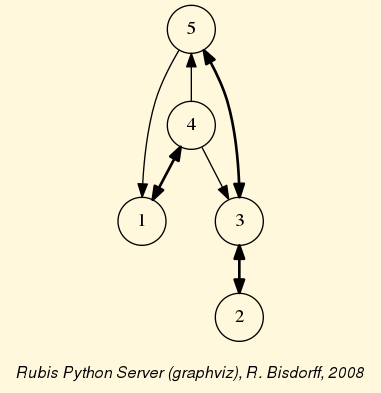
\includegraphics{testdigraph.png}\hfill}
\begin{description}
\item[{Some simple methods are easily applicable to this instantiated Digraph object \emph{dg} , like the following \code{Digraph.showStatistics()} method:}] \leavevmode
\begin{Verbatim}[commandchars=\\\{\}]
\PYG{g+gp}{\PYGZgt{}\PYGZgt{}\PYGZgt{} }\PYG{n}{dg}\PYG{o}{.}\PYG{n}{showStatistics}\PYG{p}{(}\PYG{p}{)}
\PYG{g+go}{*\PYGZhy{}\PYGZhy{}\PYGZhy{}\PYGZhy{}\PYGZhy{} general statistics \PYGZhy{}\PYGZhy{}\PYGZhy{}\PYGZhy{}\PYGZhy{}\PYGZhy{}\PYGZhy{}\PYGZhy{}\PYGZhy{}\PYGZhy{}\PYGZhy{}\PYGZhy{}\PYGZhy{}*}
\PYG{g+go}{for digraph             : \PYGZlt{}tutorialdigraph.py\PYGZgt{}}
\PYG{g+go}{order                   :  5 nodes}
\PYG{g+go}{size                    :  9 arcs}
\PYG{g+go}{\PYGZsh{} undetermined          :  0 arcs}
\PYG{g+go}{arc density             : 45.00}
\PYG{g+go}{\PYGZsh{} components            :  1}
\PYG{g+go}{                        :  [0, 1, 2, 3, 4]}
\PYG{g+go}{outdegrees distribution :  [0, 2, 2, 1, 0]}
\PYG{g+go}{indegrees distribution  :  [0, 2, 2, 1, 0]}
\PYG{g+go}{degrees distribution    :  [0, 4, 4, 2, 0]}
\PYG{g+go}{mean degree : 1.80}
\PYG{g+go}{                                  :  [0, 1, 2, 3, 4, \PYGZsq{}inf\PYGZsq{}]}
\PYG{g+go}{neighbourhood\PYGZhy{}depths distribution :  [0, 0, 2, 2, 1, 0]}
\PYG{g+go}{mean neighbourhood depth : 2.80}
\PYG{g+go}{digraph diameter :  4}
\PYG{g+go}{agglomeration distribution :}
\PYG{g+go}{1 : 50.00}
\PYG{g+go}{2 : 0.00}
\PYG{g+go}{3 : 16.67}
\PYG{g+go}{4 : 50.00}
\PYG{g+go}{5 : 50.00}
\PYG{g+go}{agglomeration coefficient : 33.33}
\PYG{g+gp}{\PYGZgt{}\PYGZgt{}\PYGZgt{} }\PYG{o}{.}\PYG{o}{.}\PYG{o}{.}
\end{Verbatim}

\end{description}


\subsubsection{Special classes of digraphs}
\label{tutorial:special-classes-of-digraphs}\begin{description}
\item[{Some special classes of digraphs, like the \code{CompleteDigraph}, the \code{EmptyDigraph} or the oriented \code{GridDigraph} class for instance, are readily available:}] \leavevmode
\begin{Verbatim}[commandchars=\\\{\}]
\PYG{g+gp}{\PYGZgt{}\PYGZgt{}\PYGZgt{} }\PYG{k+kn}{from} \PYG{n+nn}{digraphs} \PYG{k+kn}{import} \PYG{n}{GridDigraph}
\PYG{g+gp}{\PYGZgt{}\PYGZgt{}\PYGZgt{} }\PYG{n}{grid} \PYG{o}{=} \PYG{n}{GridDigraph}\PYG{p}{(}\PYG{n}{n}\PYG{o}{=}\PYG{l+m+mi}{5}\PYG{p}{,}\PYG{n}{m}\PYG{o}{=}\PYG{l+m+mi}{5}\PYG{p}{,}\PYG{n}{hasMedianSplitOrientation}\PYG{o}{=}\PYG{n+nb+bp}{True}\PYG{p}{)}
\PYG{g+gp}{\PYGZgt{}\PYGZgt{}\PYGZgt{} }\PYG{n}{grid}\PYG{o}{.}\PYG{n}{exportGraphViz}\PYG{p}{(}\PYG{l+s}{\PYGZsq{}}\PYG{l+s}{tutorialGrid}\PYG{l+s}{\PYGZsq{}}\PYG{p}{)}
\PYG{g+go}{*\PYGZhy{}\PYGZhy{}\PYGZhy{}\PYGZhy{} exporting a dot file for GraphViz tools \PYGZhy{}\PYGZhy{}\PYGZhy{}\PYGZhy{}\PYGZhy{}\PYGZhy{}\PYGZhy{}\PYGZhy{}\PYGZhy{}*}
\PYG{g+go}{Exporting to tutorialGrid.dot}
\PYG{g+go}{dot \PYGZhy{}Grankdir=BT \PYGZhy{}Tpng TutorialGrid.dot \PYGZhy{}o tutorialGrid.png}
\end{Verbatim}

\end{description}

{\hfill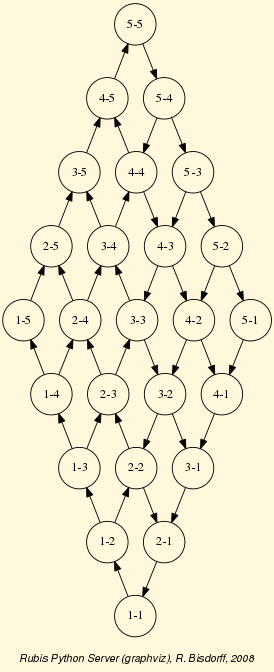
\includegraphics{tutorialGrid.png}\hfill}

For more information about its resources, see the technical documentation of the {\hyperref[techDoc:digraphs-label]{\emph{digraphs module}}} .

Back to {\hyperref[tutorial:tutorial-label]{\emph{Content}}}


\subsection{Tools for manipulating \texttt{Digraph} objects}
\label{tutorial:digraph-tools-label}\label{tutorial:tools-for-manipulating-digraph-objects}

\subsubsection{Inspecting a random digraph}
\label{tutorial:inspecting-a-random-digraph}\begin{description}
\item[{We are starting this tutorial with generating a randomly {[}-1;1{]}-valued (\emph{Normalized=True}) digraph of order 7, denoted \emph{dg} and modelling a binary relation (\emph{x S y}) defined on the set of nodes of \emph{dg}. For this purpose, the \code{digraphs} module provides conveniently a specific \code{RandomValuationDigraph} constructor:}] \leavevmode
\begin{Verbatim}[commandchars=\\\{\}]
\PYG{g+gp}{\PYGZgt{}\PYGZgt{}\PYGZgt{} }\PYG{k+kn}{from} \PYG{n+nn}{digraphs} \PYG{k+kn}{import} \PYG{n}{RandomValuationDigraph}
\PYG{g+gp}{\PYGZgt{}\PYGZgt{}\PYGZgt{} }\PYG{n}{dg} \PYG{o}{=} \PYG{n}{RandomValuationDigraph}\PYG{p}{(}\PYG{n}{order}\PYG{o}{=}\PYG{l+m+mi}{7}\PYG{p}{,}\PYG{n}{Normalized}\PYG{o}{=}\PYG{n+nb+bp}{True}\PYG{p}{)}
\PYG{g+gp}{\PYGZgt{}\PYGZgt{}\PYGZgt{} }\PYG{n}{dg}\PYG{o}{.}\PYG{n}{save}\PYG{p}{(}\PYG{l+s}{\PYGZsq{}}\PYG{l+s}{tutRandValDigraph}\PYG{l+s}{\PYGZsq{}}\PYG{p}{)}
\end{Verbatim}

\item[{With the \code{save()} method we may keep a backup version for future use of \emph{dg} which will be stored in a file called \emph{tutRandValDigraph.py} in the current working directory. The \code{Digraph} class now provides some generic methods for exploring a given \code{Digraph} object, like the \code{showShort()}, \code{showAll()}, \code{showRelationTable()} and the \code{showNeighborhoods()} methods:}] \leavevmode
\begin{Verbatim}[commandchars=\\\{\}]
\PYG{g+gp}{\PYGZgt{}\PYGZgt{}\PYGZgt{} }\PYG{n}{dg}\PYG{o}{.}\PYG{n}{showShort}\PYG{p}{(}\PYG{p}{)}
\PYG{g+go}{*\PYGZhy{}\PYGZhy{}\PYGZhy{}\PYGZhy{}\PYGZhy{} show summary \PYGZhy{}\PYGZhy{}\PYGZhy{}\PYGZhy{}\PYGZhy{}\PYGZhy{}\PYGZhy{}\PYGZhy{}\PYGZhy{}\PYGZhy{}\PYGZhy{}\PYGZhy{}\PYGZhy{}*}
\PYG{g+go}{Digraph          : randomValuationDigraph}
\PYG{g+go}{*\PYGZhy{}\PYGZhy{}\PYGZhy{}\PYGZhy{} Actions \PYGZhy{}\PYGZhy{}\PYGZhy{}\PYGZhy{}*}
\PYG{g+go}{[\PYGZsq{}1\PYGZsq{}, \PYGZsq{}2\PYGZsq{}, \PYGZsq{}3\PYGZsq{}, \PYGZsq{}4\PYGZsq{}, \PYGZsq{}5\PYGZsq{}, \PYGZsq{}6\PYGZsq{}, \PYGZsq{}7\PYGZsq{}]}
\PYG{g+go}{*\PYGZhy{}\PYGZhy{}\PYGZhy{}\PYGZhy{} Characteristic valuation domain \PYGZhy{}\PYGZhy{}\PYGZhy{}\PYGZhy{}*}
\PYG{g+go}{\PYGZob{}\PYGZsq{}med\PYGZsq{}: Decimal(\PYGZsq{}0.0\PYGZsq{}), \PYGZsq{}hasIntegerValuation\PYGZsq{}: False,}
\PYG{g+go}{\PYGZsq{}min\PYGZsq{}: Decimal(\PYGZsq{}\PYGZhy{}1.0\PYGZsq{}), \PYGZsq{}max\PYGZsq{}: Decimal(\PYGZsq{}1.0\PYGZsq{})\PYGZcb{}}
\PYG{g+go}{*\PYGZhy{}\PYGZhy{}\PYGZhy{} Connected Components \PYGZhy{}\PYGZhy{}\PYGZhy{}*}
\PYG{g+go}{1: [\PYGZsq{}1\PYGZsq{}, \PYGZsq{}2\PYGZsq{}, \PYGZsq{}3\PYGZsq{}, \PYGZsq{}4\PYGZsq{}, \PYGZsq{}5\PYGZsq{}, \PYGZsq{}6\PYGZsq{}, \PYGZsq{}7\PYGZsq{}]}
\PYG{g+gp}{\PYGZgt{}\PYGZgt{}\PYGZgt{} }\PYG{n}{dg}\PYG{o}{.}\PYG{n}{showRelationTable}\PYG{p}{(}\PYG{n}{ReflexiveTerms}\PYG{o}{=}\PYG{n+nb+bp}{False}\PYG{p}{)}
\PYG{g+go}{* \PYGZhy{}\PYGZhy{}\PYGZhy{}\PYGZhy{} Relation Table \PYGZhy{}\PYGZhy{}\PYGZhy{}\PYGZhy{}\PYGZhy{}}
\PYG{g+go}{r(xSy) \textbar{}  \PYGZsq{}1\PYGZsq{}    \PYGZsq{}2\PYGZsq{}   \PYGZsq{}3\PYGZsq{}  \PYGZsq{}4\PYGZsq{}   \PYGZsq{}5\PYGZsq{}    \PYGZsq{}6\PYGZsq{}  \PYGZsq{}7\PYGZsq{}}
\PYG{g+go}{\PYGZhy{}\PYGZhy{}\PYGZhy{}\PYGZhy{}\PYGZhy{}\PYGZhy{}\PYGZhy{}\textbar{}\PYGZhy{}\PYGZhy{}\PYGZhy{}\PYGZhy{}\PYGZhy{}\PYGZhy{}\PYGZhy{}\PYGZhy{}\PYGZhy{}\PYGZhy{}\PYGZhy{}\PYGZhy{}\PYGZhy{}\PYGZhy{}\PYGZhy{}\PYGZhy{}\PYGZhy{}\PYGZhy{}\PYGZhy{}\PYGZhy{}\PYGZhy{}\PYGZhy{}\PYGZhy{}\PYGZhy{}\PYGZhy{}\PYGZhy{}\PYGZhy{}\PYGZhy{}\PYGZhy{}\PYGZhy{}\PYGZhy{}\PYGZhy{}\PYGZhy{}\PYGZhy{}\PYGZhy{}\PYGZhy{}\PYGZhy{}\PYGZhy{}\PYGZhy{}\PYGZhy{}\PYGZhy{}\PYGZhy{}\PYGZhy{}\PYGZhy{}\PYGZhy{}\PYGZhy{}\PYGZhy{}\PYGZhy{}\PYGZhy{}\PYGZhy{}\PYGZhy{}\PYGZhy{}\PYGZhy{}\PYGZhy{}\PYGZhy{}\PYGZhy{}\PYGZhy{}\PYGZhy{}\PYGZhy{}\PYGZhy{}}
\PYG{g+go}{\PYGZsq{}1\PYGZsq{}    \textbar{}   \PYGZhy{}   \PYGZhy{}0.48  0.70  0.86  0.30  0.38  0.44}
\PYG{g+go}{\PYGZsq{}2\PYGZsq{}    \textbar{} \PYGZhy{}0.22   \PYGZhy{}   \PYGZhy{}0.38  0.50  0.80 \PYGZhy{}0.54  0.02}
\PYG{g+go}{\PYGZsq{}3\PYGZsq{}    \textbar{} \PYGZhy{}0.42  0.08   \PYGZhy{}    0.70 \PYGZhy{}0.56  0.84 \PYGZhy{}1.00}
\PYG{g+go}{\PYGZsq{}4\PYGZsq{}    \textbar{}  0.44 \PYGZhy{}0.40 \PYGZhy{}0.62   \PYGZhy{}    0.04  0.66  0.76}
\PYG{g+go}{\PYGZsq{}5\PYGZsq{}    \textbar{}  0.32 \PYGZhy{}0.48 \PYGZhy{}0.46  0.64   \PYGZhy{}   \PYGZhy{}0.22 \PYGZhy{}0.52}
\PYG{g+go}{\PYGZsq{}6\PYGZsq{}    \textbar{} \PYGZhy{}0.84  0.00 \PYGZhy{}0.40 \PYGZhy{}0.96 \PYGZhy{}0.18   \PYGZhy{}   \PYGZhy{}0.22}
\PYG{g+go}{\PYGZsq{}7\PYGZsq{}    \textbar{}  0.88  0.72  0.82  0.52 \PYGZhy{}0.84  0.04  \PYGZhy{}}
\PYG{g+gp}{\PYGZgt{}\PYGZgt{}\PYGZgt{} }\PYG{n}{dg}\PYG{o}{.}\PYG{n}{showNeighborhoods}\PYG{p}{(}\PYG{p}{)}
\PYG{g+go}{Neighborhoods osberved in digraph \PYGZsq{}randomdomValuation\PYGZsq{}}
\PYG{g+go}{Gamma     :}
\PYG{g+go}{\PYGZsq{}1\PYGZsq{}: in =\PYGZgt{} \PYGZob{}\PYGZsq{}5\PYGZsq{}, \PYGZsq{}7\PYGZsq{}, \PYGZsq{}4\PYGZsq{}\PYGZcb{}, out =\PYGZgt{} \PYGZob{}\PYGZsq{}5\PYGZsq{}, \PYGZsq{}7\PYGZsq{}, \PYGZsq{}6\PYGZsq{}, \PYGZsq{}3\PYGZsq{}, \PYGZsq{}4\PYGZsq{}\PYGZcb{}}
\PYG{g+go}{\PYGZsq{}2\PYGZsq{}: in =\PYGZgt{} \PYGZob{}\PYGZsq{}7\PYGZsq{}, \PYGZsq{}3\PYGZsq{}\PYGZcb{}, out =\PYGZgt{} \PYGZob{}\PYGZsq{}5\PYGZsq{}, \PYGZsq{}7\PYGZsq{}, \PYGZsq{}4\PYGZsq{}\PYGZcb{}}
\PYG{g+go}{\PYGZsq{}3\PYGZsq{}: in =\PYGZgt{} \PYGZob{}\PYGZsq{}7\PYGZsq{}, \PYGZsq{}1\PYGZsq{}\PYGZcb{}, out =\PYGZgt{} \PYGZob{}\PYGZsq{}6\PYGZsq{}, \PYGZsq{}2\PYGZsq{}, \PYGZsq{}4\PYGZsq{}\PYGZcb{}}
\PYG{g+go}{\PYGZsq{}4\PYGZsq{}: in =\PYGZgt{} \PYGZob{}\PYGZsq{}5\PYGZsq{}, \PYGZsq{}7\PYGZsq{}, \PYGZsq{}1\PYGZsq{}, \PYGZsq{}2\PYGZsq{}, \PYGZsq{}3\PYGZsq{}\PYGZcb{}, out =\PYGZgt{} \PYGZob{}\PYGZsq{}5\PYGZsq{}, \PYGZsq{}7\PYGZsq{}, \PYGZsq{}1\PYGZsq{}, \PYGZsq{}6\PYGZsq{}\PYGZcb{}}
\PYG{g+go}{\PYGZsq{}5\PYGZsq{}: in =\PYGZgt{} \PYGZob{}\PYGZsq{}1\PYGZsq{}, \PYGZsq{}2\PYGZsq{}, \PYGZsq{}4\PYGZsq{}\PYGZcb{}, out =\PYGZgt{} \PYGZob{}\PYGZsq{}1\PYGZsq{}, \PYGZsq{}4\PYGZsq{}\PYGZcb{}}
\PYG{g+go}{\PYGZsq{}6\PYGZsq{}: in =\PYGZgt{} \PYGZob{}\PYGZsq{}7\PYGZsq{}, \PYGZsq{}1\PYGZsq{}, \PYGZsq{}3\PYGZsq{}, \PYGZsq{}4\PYGZsq{}\PYGZcb{}, out =\PYGZgt{} set()}
\PYG{g+go}{\PYGZsq{}7\PYGZsq{}: in =\PYGZgt{} \PYGZob{}\PYGZsq{}1\PYGZsq{}, \PYGZsq{}2\PYGZsq{}, \PYGZsq{}4\PYGZsq{}\PYGZcb{}, out =\PYGZgt{} \PYGZob{}\PYGZsq{}1\PYGZsq{}, \PYGZsq{}2\PYGZsq{}, \PYGZsq{}3\PYGZsq{}, \PYGZsq{}4\PYGZsq{}, \PYGZsq{}6\PYGZsq{}\PYGZcb{}}
\PYG{g+go}{ Not Gamma :}
\PYG{g+go}{\PYGZsq{}1\PYGZsq{}: in =\PYGZgt{} \PYGZob{}\PYGZsq{}6\PYGZsq{}, \PYGZsq{}2\PYGZsq{}, \PYGZsq{}3\PYGZsq{}\PYGZcb{}, out =\PYGZgt{} \PYGZob{}\PYGZsq{}2\PYGZsq{}\PYGZcb{}}
\PYG{g+go}{\PYGZsq{}2\PYGZsq{}: in =\PYGZgt{} \PYGZob{}\PYGZsq{}5\PYGZsq{}, \PYGZsq{}1\PYGZsq{}, \PYGZsq{}4\PYGZsq{}\PYGZcb{}, out =\PYGZgt{} \PYGZob{}\PYGZsq{}1\PYGZsq{}, \PYGZsq{}6\PYGZsq{}, \PYGZsq{}3\PYGZsq{}\PYGZcb{}}
\PYG{g+go}{\PYGZsq{}3\PYGZsq{}: in =\PYGZgt{} \PYGZob{}\PYGZsq{}5\PYGZsq{}, \PYGZsq{}6\PYGZsq{}, \PYGZsq{}2\PYGZsq{}, \PYGZsq{}4\PYGZsq{}\PYGZcb{}, out =\PYGZgt{} \PYGZob{}\PYGZsq{}5\PYGZsq{}, \PYGZsq{}7\PYGZsq{}, \PYGZsq{}1\PYGZsq{}\PYGZcb{}}
\PYG{g+go}{\PYGZsq{}4\PYGZsq{}: in =\PYGZgt{} \PYGZob{}\PYGZsq{}6\PYGZsq{}\PYGZcb{}, out =\PYGZgt{} \PYGZob{}\PYGZsq{}2\PYGZsq{}, \PYGZsq{}3\PYGZsq{}\PYGZcb{}}
\PYG{g+go}{\PYGZsq{}5\PYGZsq{}: in =\PYGZgt{} \PYGZob{}\PYGZsq{}7\PYGZsq{}, \PYGZsq{}6\PYGZsq{}, \PYGZsq{}3\PYGZsq{}\PYGZcb{}, out =\PYGZgt{} \PYGZob{}\PYGZsq{}7\PYGZsq{}, \PYGZsq{}6\PYGZsq{}, \PYGZsq{}2\PYGZsq{}, \PYGZsq{}3\PYGZsq{}\PYGZcb{}}
\PYG{g+go}{\PYGZsq{}6\PYGZsq{}: in =\PYGZgt{} \PYGZob{}\PYGZsq{}5\PYGZsq{}, \PYGZsq{}2\PYGZsq{}\PYGZcb{}, out =\PYGZgt{} \PYGZob{}\PYGZsq{}5\PYGZsq{}, \PYGZsq{}7\PYGZsq{}, \PYGZsq{}1\PYGZsq{}, \PYGZsq{}3\PYGZsq{}, \PYGZsq{}4\PYGZsq{}\PYGZcb{}}
\PYG{g+go}{\PYGZsq{}7\PYGZsq{}: in =\PYGZgt{} \PYGZob{}\PYGZsq{}5\PYGZsq{}, \PYGZsq{}6\PYGZsq{}, \PYGZsq{}3\PYGZsq{}\PYGZcb{}, out =\PYGZgt{} \PYGZob{}\PYGZsq{}5\PYGZsq{}\PYGZcb{}}
\end{Verbatim}

\end{description}

\begin{notice}{warning}{Warning:}
Notice that most Digraph class methods will ignore the reflexive couples by considering that the relation is indeterminate (the characteristic value \emph{r(x S x)} for all action \emph{x} is put to the median, i.e. indeterminate, value) in this case.
\end{notice}


\subsubsection{Graphviz drawings}
\label{tutorial:graphviz-drawings}\begin{description}
\item[{We may have an even better insight into the \code{Digraph} object \emph{dg} by looking at a \href{http://graphviz.org/}{graphviz} \footnote{
The \code{exportGraphViz} method is depending on drawing tools from \href{http://graphviz.org/}{graphviz}. On Linux Ubuntu or Debian you may try \code{sudo apt-get install graphviz} to install them. There are ready \code{dmg} installers for Mac OS.
} drawing:}] \leavevmode
\begin{Verbatim}[commandchars=\\\{\}]
\PYG{g+gp}{\PYGZgt{}\PYGZgt{}\PYGZgt{} }\PYG{n}{dg}\PYG{o}{.}\PYG{n}{exportGraphViz}\PYG{p}{(}\PYG{l+s}{\PYGZsq{}}\PYG{l+s}{tutRandValDigraph}\PYG{l+s}{\PYGZsq{}}\PYG{p}{)}
\PYG{g+go}{*\PYGZhy{}\PYGZhy{}\PYGZhy{}\PYGZhy{} exporting a dot file for GraphViz tools \PYGZhy{}\PYGZhy{}\PYGZhy{}\PYGZhy{}\PYGZhy{}\PYGZhy{}\PYGZhy{}\PYGZhy{}\PYGZhy{}*}
\PYG{g+go}{Exporting to tutRandValDigraph.dot}
\PYG{g+go}{dot \PYGZhy{}Grankdir=BT \PYGZhy{}Tpng tutRandValDigraph.dot \PYGZhy{}o tutRandValDigraph.png}
\end{Verbatim}

\end{description}

{\hfill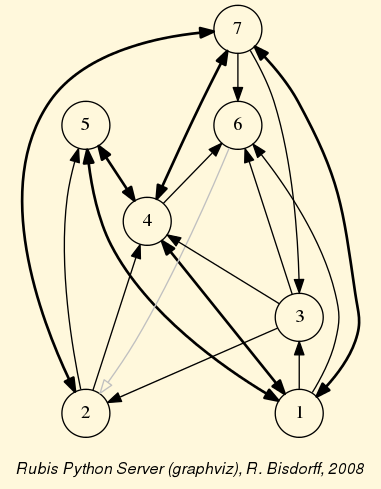
\includegraphics{tutRandValDigraph.png}\hfill}

Double links are drawn in bold black with an arrowhead at each end, whereas single asymmetric links are drawn in black with an arrowhead showing the direction of the link. Notice the undetermined relational situation (\emph{r(6 S 2) = 0.00}) observed between nodes `6' and `2'. The corresponding link is marked in gray with an open arrowhead in the drawing.


\subsubsection{Asymmetric and symmetric parts}
\label{tutorial:asymmetric-and-symmetric-parts}\begin{description}
\item[{We may now extract both this symmetric as well as this asymmetric part of digraph \emph{dg} with the help of two corresponding constructors:}] \leavevmode
\begin{Verbatim}[commandchars=\\\{\}]
\PYG{g+gp}{\PYGZgt{}\PYGZgt{}\PYGZgt{} }\PYG{k+kn}{from} \PYG{n+nn}{digraphs} \PYG{k+kn}{import} \PYG{n}{AsymmetricPartialDigraph}\PYG{p}{,} \PYG{n}{SymmetricPartialDigraph}
\PYG{g+gp}{\PYGZgt{}\PYGZgt{}\PYGZgt{} }\PYG{n}{asymDg} \PYG{o}{=} \PYG{n}{AsymmetricPartialDigraph}\PYG{p}{(}\PYG{n}{dg}\PYG{p}{)}
\PYG{g+gp}{\PYGZgt{}\PYGZgt{}\PYGZgt{} }\PYG{n}{asymDg}\PYG{o}{.}\PYG{n}{exportGraphViz}\PYG{p}{(}\PYG{p}{)}
\PYG{g+gp}{\PYGZgt{}\PYGZgt{}\PYGZgt{} }\PYG{n}{symDG} \PYG{o}{=} \PYG{n}{SymmetricPartialDigraph}\PYG{p}{(}\PYG{n}{dg}\PYG{p}{)}
\PYG{g+gp}{\PYGZgt{}\PYGZgt{}\PYGZgt{} }\PYG{n}{symDg}\PYG{o}{.}\PYG{n}{exportGraphViz}\PYG{p}{(}\PYG{p}{)}
\end{Verbatim}

\end{description}

{\hfill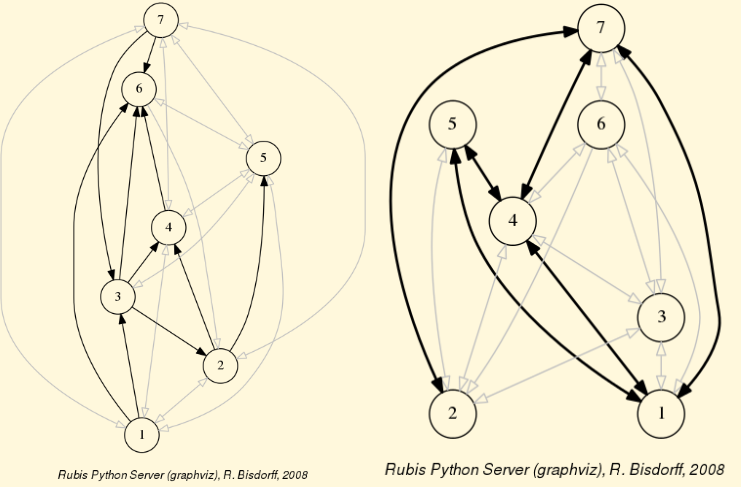
\includegraphics{asymSymParts.png}\hfill}

\begin{notice}{note}{Note:}
Notice that the partial objects \emph{asymDg} and \emph{symDg} put to the indeterminate characteristic value all not-asymmetric, respectively not-symmetric links between nodes.
\end{notice}

Here below, for illustration the source code of \emph{relation} constructor of the \code{AsymmetricPartialDigraph} class:

\begin{Verbatim}[commandchars=\\\{\}]
\PYG{k}{def} \PYG{n+nf}{\PYGZus{}constructRelation}\PYG{p}{(}\PYG{n+nb+bp}{self}\PYG{p}{)}\PYG{p}{:}
    \PYG{n}{actions} \PYG{o}{=} \PYG{n+nb+bp}{self}\PYG{o}{.}\PYG{n}{actions}
    \PYG{n}{Min} \PYG{o}{=} \PYG{n+nb+bp}{self}\PYG{o}{.}\PYG{n}{valuationdomain}\PYG{p}{[}\PYG{l+s}{\PYGZsq{}}\PYG{l+s}{min}\PYG{l+s}{\PYGZsq{}}\PYG{p}{]}
    \PYG{n}{Max} \PYG{o}{=} \PYG{n+nb+bp}{self}\PYG{o}{.}\PYG{n}{valuationdomain}\PYG{p}{[}\PYG{l+s}{\PYGZsq{}}\PYG{l+s}{max}\PYG{l+s}{\PYGZsq{}}\PYG{p}{]}
    \PYG{n}{Med} \PYG{o}{=} \PYG{n+nb+bp}{self}\PYG{o}{.}\PYG{n}{valuationdomain}\PYG{p}{[}\PYG{l+s}{\PYGZsq{}}\PYG{l+s}{med}\PYG{l+s}{\PYGZsq{}}\PYG{p}{]}
    \PYG{n}{relationIn} \PYG{o}{=} \PYG{n+nb+bp}{self}\PYG{o}{.}\PYG{n}{relation}
    \PYG{n}{relationOut} \PYG{o}{=} \PYG{p}{\PYGZob{}}\PYG{p}{\PYGZcb{}}
    \PYG{k}{for} \PYG{n}{a} \PYG{o+ow}{in} \PYG{n}{actions}\PYG{p}{:}
        \PYG{n}{relationOut}\PYG{p}{[}\PYG{n}{a}\PYG{p}{]} \PYG{o}{=} \PYG{p}{\PYGZob{}}\PYG{p}{\PYGZcb{}}
        \PYG{k}{for} \PYG{n}{b} \PYG{o+ow}{in} \PYG{n}{actions}\PYG{p}{:}
            \PYG{k}{if} \PYG{n}{a} \PYG{o}{!=} \PYG{n}{b}\PYG{p}{:}
                \PYG{k}{if} \PYG{n}{relationIn}\PYG{p}{[}\PYG{n}{a}\PYG{p}{]}\PYG{p}{[}\PYG{n}{b}\PYG{p}{]} \PYG{o}{\PYGZgt{}}\PYG{o}{=} \PYG{n}{Med} \PYG{o+ow}{and} \PYG{n}{relationIn}\PYG{p}{[}\PYG{n}{b}\PYG{p}{]}\PYG{p}{[}\PYG{n}{a}\PYG{p}{]} \PYG{o}{\PYGZlt{}}\PYG{o}{=} \PYG{n}{Med}\PYG{p}{:}
                    \PYG{n}{relationOut}\PYG{p}{[}\PYG{n}{a}\PYG{p}{]}\PYG{p}{[}\PYG{n}{b}\PYG{p}{]} \PYG{o}{=} \PYG{n}{relationIn}\PYG{p}{[}\PYG{n}{a}\PYG{p}{]}\PYG{p}{[}\PYG{n}{b}\PYG{p}{]}
                \PYG{k}{elif} \PYG{n}{relationIn}\PYG{p}{[}\PYG{n}{a}\PYG{p}{]}\PYG{p}{[}\PYG{n}{b}\PYG{p}{]} \PYG{o}{\PYGZlt{}}\PYG{o}{=} \PYG{n}{Med} \PYG{o+ow}{and} \PYG{n}{relationIn}\PYG{p}{[}\PYG{n}{b}\PYG{p}{]}\PYG{p}{[}\PYG{n}{a}\PYG{p}{]} \PYG{o}{\PYGZgt{}}\PYG{o}{=} \PYG{n}{Med}\PYG{p}{:}
                    \PYG{n}{relationOut}\PYG{p}{[}\PYG{n}{a}\PYG{p}{]}\PYG{p}{[}\PYG{n}{b}\PYG{p}{]} \PYG{o}{=} \PYG{n}{relationIn}\PYG{p}{[}\PYG{n}{a}\PYG{p}{]}\PYG{p}{[}\PYG{n}{b}\PYG{p}{]}
                \PYG{k}{else}\PYG{p}{:}
                    \PYG{n}{relationOut}\PYG{p}{[}\PYG{n}{a}\PYG{p}{]}\PYG{p}{[}\PYG{n}{b}\PYG{p}{]} \PYG{o}{=} \PYG{n}{Med}
            \PYG{k}{else}\PYG{p}{:}
                \PYG{n}{relationOut}\PYG{p}{[}\PYG{n}{a}\PYG{p}{]}\PYG{p}{[}\PYG{n}{b}\PYG{p}{]} \PYG{o}{=} \PYG{n}{Med}
    \PYG{k}{return} \PYG{n}{relationOut}
\end{Verbatim}


\subsubsection{Digraph fusion by epistemic disjunction}
\label{tutorial:digraph-fusion-by-epistemic-disjunction}\begin{description}
\item[{We may recover object \emph{dg} from both partial objects \emph{asymDg} and \emph{symDg} with a \textbf{bipolar fusion} constructor, also called \textbf{epistemic disjunction}, available via the \code{FusionDigraph} class:}] \leavevmode
\begin{Verbatim}[commandchars=\\\{\}]
\PYG{g+gp}{\PYGZgt{}\PYGZgt{}\PYGZgt{} }\PYG{k+kn}{from} \PYG{n+nn}{digraphs} \PYG{k+kn}{import} \PYG{n}{FusionDigraph}
\PYG{g+gp}{\PYGZgt{}\PYGZgt{}\PYGZgt{} }\PYG{n}{fusDg} \PYG{o}{=} \PYG{n}{FusionDigraph}\PYG{p}{(}\PYG{n}{asymDg}\PYG{p}{,}\PYG{n}{symDg}\PYG{p}{)}
\PYG{g+gp}{\PYGZgt{}\PYGZgt{}\PYGZgt{} }\PYG{n}{fusDg}\PYG{o}{.}\PYG{n}{showRelationTable}\PYG{p}{(}\PYG{p}{)}
\PYG{g+go}{* \PYGZhy{}\PYGZhy{}\PYGZhy{}\PYGZhy{} Relation Table \PYGZhy{}\PYGZhy{}\PYGZhy{}\PYGZhy{}\PYGZhy{}}
\PYG{g+go}{r(xSy) \textbar{}  \PYGZsq{}1\PYGZsq{}    \PYGZsq{}2\PYGZsq{}   \PYGZsq{}3\PYGZsq{}  \PYGZsq{}4\PYGZsq{}   \PYGZsq{}5\PYGZsq{}    \PYGZsq{}6\PYGZsq{}  \PYGZsq{}7\PYGZsq{}}
\PYG{g+go}{\PYGZhy{}\PYGZhy{}\PYGZhy{}\PYGZhy{}\PYGZhy{}\PYGZhy{}\PYGZhy{}\textbar{}\PYGZhy{}\PYGZhy{}\PYGZhy{}\PYGZhy{}\PYGZhy{}\PYGZhy{}\PYGZhy{}\PYGZhy{}\PYGZhy{}\PYGZhy{}\PYGZhy{}\PYGZhy{}\PYGZhy{}\PYGZhy{}\PYGZhy{}\PYGZhy{}\PYGZhy{}\PYGZhy{}\PYGZhy{}\PYGZhy{}\PYGZhy{}\PYGZhy{}\PYGZhy{}\PYGZhy{}\PYGZhy{}\PYGZhy{}\PYGZhy{}\PYGZhy{}\PYGZhy{}\PYGZhy{}\PYGZhy{}\PYGZhy{}\PYGZhy{}\PYGZhy{}\PYGZhy{}\PYGZhy{}\PYGZhy{}\PYGZhy{}\PYGZhy{}\PYGZhy{}\PYGZhy{}\PYGZhy{}\PYGZhy{}\PYGZhy{}\PYGZhy{}\PYGZhy{}\PYGZhy{}\PYGZhy{}\PYGZhy{}\PYGZhy{}\PYGZhy{}\PYGZhy{}\PYGZhy{}\PYGZhy{}\PYGZhy{}\PYGZhy{}\PYGZhy{}\PYGZhy{}\PYGZhy{}\PYGZhy{}}
\PYG{g+go}{\PYGZsq{}1\PYGZsq{}    \textbar{}  0.00 \PYGZhy{}0.48  0.70  0.86  0.30  0.38  0.44}
\PYG{g+go}{\PYGZsq{}2\PYGZsq{}    \textbar{} \PYGZhy{}0.22  0.00 \PYGZhy{}0.38  0.50  0.80 \PYGZhy{}0.54  0.02}
\PYG{g+go}{\PYGZsq{}3\PYGZsq{}    \textbar{} \PYGZhy{}0.42  0.08  0.00  0.70 \PYGZhy{}0.56  0.84 \PYGZhy{}1.00}
\PYG{g+go}{\PYGZsq{}4\PYGZsq{}    \textbar{}  0.44 \PYGZhy{}0.40 \PYGZhy{}0.62  0.00  0.04  0.66  0.76}
\PYG{g+go}{\PYGZsq{}5\PYGZsq{}    \textbar{}  0.32 \PYGZhy{}0.48 \PYGZhy{}0.46  0.64  0.00 \PYGZhy{}0.22 \PYGZhy{}0.52}
\PYG{g+go}{\PYGZsq{}6\PYGZsq{}    \textbar{} \PYGZhy{}0.84  0.00 \PYGZhy{}0.40 \PYGZhy{}0.96 \PYGZhy{}0.18  0.00 \PYGZhy{}0.22}
\PYG{g+go}{\PYGZsq{}7\PYGZsq{}    \textbar{}  0.88  0.72  0.82  0.52 \PYGZhy{}0.84  0.04  0.00}
\end{Verbatim}

\end{description}


\subsubsection{Dual, converse and codual digraphs}
\label{tutorial:dual-converse-and-codual-digraphs}\begin{description}
\item[{We may as readily compute the \textbf{dual}, the \textbf{converse} and the \textbf{codual} (dual and converse) of \emph{dg}:}] \leavevmode
\begin{Verbatim}[commandchars=\\\{\}]
\PYG{g+gp}{\PYGZgt{}\PYGZgt{}\PYGZgt{} }\PYG{k+kn}{from} \PYG{n+nn}{digraphs} \PYG{k+kn}{import} \PYG{n}{DualDigraph}\PYG{p}{,} \PYG{n}{ConverseDigraph}\PYG{p}{,} \PYG{n}{CoDualDigraph}
\PYG{g+gp}{\PYGZgt{}\PYGZgt{}\PYGZgt{} }\PYG{n}{ddg} \PYG{o}{=} \PYG{n}{DualDigraph}\PYG{p}{(}\PYG{n}{dg}\PYG{p}{)}
\PYG{g+gp}{\PYGZgt{}\PYGZgt{}\PYGZgt{} }\PYG{n}{ddg}\PYG{o}{.}\PYG{n}{showRelationTable}\PYG{p}{(}\PYG{p}{)}
\PYG{g+go}{\PYGZhy{}r(xSy) \textbar{}  \PYGZsq{}1\PYGZsq{}    \PYGZsq{}2\PYGZsq{}   \PYGZsq{}3\PYGZsq{}  \PYGZsq{}4\PYGZsq{}   \PYGZsq{}5\PYGZsq{}    \PYGZsq{}6\PYGZsq{}  \PYGZsq{}7\PYGZsq{}}
\PYG{g+go}{\PYGZhy{}\PYGZhy{}\PYGZhy{}\PYGZhy{}\PYGZhy{}\PYGZhy{}\PYGZhy{}\PYGZhy{}\textbar{}\PYGZhy{}\PYGZhy{}\PYGZhy{}\PYGZhy{}\PYGZhy{}\PYGZhy{}\PYGZhy{}\PYGZhy{}\PYGZhy{}\PYGZhy{}\PYGZhy{}\PYGZhy{}\PYGZhy{}\PYGZhy{}\PYGZhy{}\PYGZhy{}\PYGZhy{}\PYGZhy{}\PYGZhy{}\PYGZhy{}\PYGZhy{}\PYGZhy{}\PYGZhy{}\PYGZhy{}\PYGZhy{}\PYGZhy{}\PYGZhy{}\PYGZhy{}\PYGZhy{}\PYGZhy{}\PYGZhy{}\PYGZhy{}\PYGZhy{}\PYGZhy{}\PYGZhy{}\PYGZhy{}\PYGZhy{}\PYGZhy{}\PYGZhy{}\PYGZhy{}\PYGZhy{}\PYGZhy{}}
\PYG{g+go}{\PYGZsq{}1 \PYGZsq{}    \textbar{}  0.00  0.48 \PYGZhy{}0.70 \PYGZhy{}0.86 \PYGZhy{}0.30 \PYGZhy{}0.38 \PYGZhy{}0.44}
\PYG{g+go}{\PYGZsq{}2\PYGZsq{}     \textbar{}  0.22  0.00  0.38 \PYGZhy{}0.50  0.80  0.54 \PYGZhy{}0.02}
\PYG{g+go}{\PYGZsq{}3\PYGZsq{}     \textbar{}  0.42  0.08  0.00 \PYGZhy{}0.70  0.56 \PYGZhy{}0.84  1.00}
\PYG{g+go}{\PYGZsq{}4\PYGZsq{}     \textbar{} \PYGZhy{}0.44  0.40  0.62  0.00 \PYGZhy{}0.04 \PYGZhy{}0.66 \PYGZhy{}0.76}
\PYG{g+go}{\PYGZsq{}5\PYGZsq{}     \textbar{} \PYGZhy{}0.32  0.48  0.46 \PYGZhy{}0.64  0.00  0.22  0.52}
\PYG{g+go}{\PYGZsq{}6\PYGZsq{}     \textbar{}  0.84  0.00  0.40  0.96  0.18  0.00  0.22}
\PYG{g+go}{\PYGZsq{}7\PYGZsq{}     \textbar{}  0.88 \PYGZhy{}0.72 \PYGZhy{}0.82 \PYGZhy{}0.52  0.84 \PYGZhy{}0.04  0.00}
\PYG{g+gp}{\PYGZgt{}\PYGZgt{}\PYGZgt{} }\PYG{n}{cdg} \PYG{o}{=} \PYG{n}{ConverseDigraph}\PYG{p}{(}\PYG{n}{dg}\PYG{p}{)}
\PYG{g+gp}{\PYGZgt{}\PYGZgt{}\PYGZgt{} }\PYG{n}{cdg}\PYG{o}{.}\PYG{n}{showRelationTable}\PYG{p}{(}\PYG{p}{)}
\PYG{g+go}{* \PYGZhy{}\PYGZhy{}\PYGZhy{}\PYGZhy{} Relation Table \PYGZhy{}\PYGZhy{}\PYGZhy{}\PYGZhy{}\PYGZhy{}}
\PYG{g+go}{ r(ySx) \textbar{}  \PYGZsq{}1\PYGZsq{}    \PYGZsq{}2\PYGZsq{}   \PYGZsq{}3\PYGZsq{}   \PYGZsq{}4\PYGZsq{}   \PYGZsq{}5\PYGZsq{}   \PYGZsq{}6\PYGZsq{}   \PYGZsq{}7\PYGZsq{}}
\PYG{g+go}{\PYGZhy{}\PYGZhy{}\PYGZhy{}\PYGZhy{}\PYGZhy{}\PYGZhy{}\PYGZhy{}\PYGZhy{}\textbar{}\PYGZhy{}\PYGZhy{}\PYGZhy{}\PYGZhy{}\PYGZhy{}\PYGZhy{}\PYGZhy{}\PYGZhy{}\PYGZhy{}\PYGZhy{}\PYGZhy{}\PYGZhy{}\PYGZhy{}\PYGZhy{}\PYGZhy{}\PYGZhy{}\PYGZhy{}\PYGZhy{}\PYGZhy{}\PYGZhy{}\PYGZhy{}\PYGZhy{}\PYGZhy{}\PYGZhy{}\PYGZhy{}\PYGZhy{}\PYGZhy{}\PYGZhy{}\PYGZhy{}\PYGZhy{}\PYGZhy{}\PYGZhy{}\PYGZhy{}\PYGZhy{}\PYGZhy{}\PYGZhy{}\PYGZhy{}\PYGZhy{}\PYGZhy{}\PYGZhy{}\PYGZhy{}\PYGZhy{}}
\PYG{g+go}{\PYGZsq{}1\PYGZsq{}     \textbar{}  0.00 \PYGZhy{}0.22 \PYGZhy{}0.42  0.44  0.32 \PYGZhy{}0.84  0.88}
\PYG{g+go}{\PYGZsq{}2\PYGZsq{}     \textbar{} \PYGZhy{}0.48  0.00  0.08 \PYGZhy{}0.40 \PYGZhy{}0.48  0.00  0.72}
\PYG{g+go}{\PYGZsq{}3\PYGZsq{}     \textbar{}  0.70 \PYGZhy{}0.38  0.00 \PYGZhy{}0.62 \PYGZhy{}0.46 \PYGZhy{}0.40  0.82}
\PYG{g+go}{\PYGZsq{}4\PYGZsq{}     \textbar{}  0.86  0.50  0.70  0.00  0.64 \PYGZhy{}0.96  0.52}
\PYG{g+go}{\PYGZsq{}5\PYGZsq{}     \textbar{}  0.30  0.80 \PYGZhy{}0.56  0.04  0.00 \PYGZhy{}0.18 \PYGZhy{}0.84}
\PYG{g+go}{\PYGZsq{}6\PYGZsq{}     \textbar{}  0.38 \PYGZhy{}0.54  0.84  0.66 \PYGZhy{}0.22  0.00  0.04}
\PYG{g+go}{\PYGZsq{}7\PYGZsq{}     \textbar{}  0.44  0.02 \PYGZhy{}1.00  0.76 \PYGZhy{}0.52 \PYGZhy{}0.22  0.00}
\PYG{g+gp}{\PYGZgt{}\PYGZgt{}\PYGZgt{} }\PYG{n}{cddg} \PYG{o}{=} \PYG{n}{CoDualDigraph}\PYG{p}{(}\PYG{n}{dg}\PYG{p}{)}
\PYG{g+gp}{\PYGZgt{}\PYGZgt{}\PYGZgt{} }\PYG{n}{cddg}\PYG{o}{.}\PYG{n}{showRelationTable}\PYG{p}{(}\PYG{p}{)}
\PYG{g+go}{* \PYGZhy{}\PYGZhy{}\PYGZhy{}\PYGZhy{} Relation Table \PYGZhy{}\PYGZhy{}\PYGZhy{}\PYGZhy{}\PYGZhy{}}
\PYG{g+go}{\PYGZhy{}r(ySx) \textbar{}  \PYGZsq{}1\PYGZsq{}    \PYGZsq{}2\PYGZsq{}   \PYGZsq{}3\PYGZsq{}   \PYGZsq{}4\PYGZsq{}   \PYGZsq{}5\PYGZsq{}   \PYGZsq{}6\PYGZsq{}   \PYGZsq{}7\PYGZsq{}}
\PYG{g+go}{\PYGZhy{}\PYGZhy{}\PYGZhy{}\PYGZhy{}\PYGZhy{}\PYGZhy{}\PYGZhy{}\PYGZhy{}\textbar{}\PYGZhy{}\PYGZhy{}\PYGZhy{}\PYGZhy{}\PYGZhy{}\PYGZhy{}\PYGZhy{}\PYGZhy{}\PYGZhy{}\PYGZhy{}\PYGZhy{}\PYGZhy{}\PYGZhy{}\PYGZhy{}\PYGZhy{}\PYGZhy{}\PYGZhy{}\PYGZhy{}\PYGZhy{}\PYGZhy{}\PYGZhy{}\PYGZhy{}\PYGZhy{}\PYGZhy{}\PYGZhy{}\PYGZhy{}\PYGZhy{}\PYGZhy{}\PYGZhy{}\PYGZhy{}\PYGZhy{}\PYGZhy{}\PYGZhy{}\PYGZhy{}\PYGZhy{}\PYGZhy{}\PYGZhy{}\PYGZhy{}\PYGZhy{}\PYGZhy{}\PYGZhy{}\PYGZhy{}\PYGZhy{}\PYGZhy{}\PYGZhy{}\PYGZhy{}\PYGZhy{}\PYGZhy{}\PYGZhy{}\PYGZhy{}\PYGZhy{}\PYGZhy{}\PYGZhy{}\PYGZhy{}\PYGZhy{}\PYGZhy{}\PYGZhy{}\PYGZhy{}\PYGZhy{}\PYGZhy{}}
\PYG{g+go}{\PYGZsq{}1\PYGZsq{}     \textbar{}  0.00  0.22  0.42 \PYGZhy{}0.44 \PYGZhy{}0.32  0.84 \PYGZhy{}0.88}
\PYG{g+go}{\PYGZsq{}2\PYGZsq{}     \textbar{}  0.48  0.00 \PYGZhy{}0.08  0.40  0.48  0.00 \PYGZhy{}0.72}
\PYG{g+go}{\PYGZsq{}3\PYGZsq{}     \textbar{} \PYGZhy{}0.70  0.38  0.00  0.62  0.46  0.40 \PYGZhy{}0.82}
\PYG{g+go}{\PYGZsq{}4\PYGZsq{}     \textbar{} \PYGZhy{}0.86 \PYGZhy{}0.50 \PYGZhy{}0.70  0.00 \PYGZhy{}0.64  0.96 \PYGZhy{}0.52}
\PYG{g+go}{\PYGZsq{}5\PYGZsq{}     \textbar{} \PYGZhy{}0.30 \PYGZhy{}0.80  0.56 \PYGZhy{}0.04  0.00  0.18  0.84}
\PYG{g+go}{\PYGZsq{}6\PYGZsq{}     \textbar{} \PYGZhy{}0.38  0.54 \PYGZhy{}0.84 \PYGZhy{}0.66  0.22  0.00 \PYGZhy{}0.04}
\PYG{g+go}{\PYGZsq{}7\PYGZsq{}     \textbar{} \PYGZhy{}0.44 \PYGZhy{}0.02  1.00 \PYGZhy{}0.76  0.52  0.22  0.00}
\end{Verbatim}

\item[{Computing the dual, respectively the converse, may also be done with prefixing the \code{\_\_neg\_\_ (-)} or the \code{\_\_invert\_\_} (\textasciitilde{}) operator. The codual of a Digraph object may, hence, as well be computed with a \textbf{composition} (in either order) of both operations:}] \leavevmode
\begin{Verbatim}[commandchars=\\\{\}]
\PYG{g+gp}{\PYGZgt{}\PYGZgt{}\PYGZgt{} }\PYG{n}{ddg} \PYG{o}{=} \PYG{o}{\PYGZhy{}}\PYG{n}{dg}   \PYG{c}{\PYGZsh{} dual of dg}
\PYG{g+gp}{\PYGZgt{}\PYGZgt{}\PYGZgt{} }\PYG{n}{cdg} \PYG{o}{=} \PYG{o}{\PYGZti{}}\PYG{n}{dg}   \PYG{c}{\PYGZsh{} converse of dg}
\PYG{g+gp}{\PYGZgt{}\PYGZgt{}\PYGZgt{} }\PYG{n}{cddg} \PYG{o}{=} \PYG{o}{\PYGZhy{}}\PYG{p}{(}\PYG{o}{\PYGZti{}}\PYG{n}{dg}\PYG{p}{)} \PYG{o}{=} \PYG{o}{\PYGZti{}}\PYG{p}{(}\PYG{o}{\PYGZhy{}}\PYG{n}{dg}\PYG{p}{)}  \PYG{c}{\PYGZsh{} codual of dg}
\PYG{g+gp}{\PYGZgt{}\PYGZgt{}\PYGZgt{} }\PYG{n}{cddg}\PYG{o}{.}\PYG{n}{showRelationTable}\PYG{p}{(}\PYG{p}{)}
\PYG{g+go}{* \PYGZhy{}\PYGZhy{}\PYGZhy{}\PYGZhy{} Relation Table \PYGZhy{}\PYGZhy{}\PYGZhy{}\PYGZhy{}\PYGZhy{}}
\PYG{g+go}{\PYGZhy{}r(ySx) \textbar{}  \PYGZsq{}1\PYGZsq{}    \PYGZsq{}2\PYGZsq{}   \PYGZsq{}3\PYGZsq{}   \PYGZsq{}4\PYGZsq{}   \PYGZsq{}5\PYGZsq{}   \PYGZsq{}6\PYGZsq{}   \PYGZsq{}7\PYGZsq{}}
\PYG{g+go}{\PYGZhy{}\PYGZhy{}\PYGZhy{}\PYGZhy{}\PYGZhy{}\PYGZhy{}\PYGZhy{}\PYGZhy{}\textbar{}\PYGZhy{}\PYGZhy{}\PYGZhy{}\PYGZhy{}\PYGZhy{}\PYGZhy{}\PYGZhy{}\PYGZhy{}\PYGZhy{}\PYGZhy{}\PYGZhy{}\PYGZhy{}\PYGZhy{}\PYGZhy{}\PYGZhy{}\PYGZhy{}\PYGZhy{}\PYGZhy{}\PYGZhy{}\PYGZhy{}\PYGZhy{}\PYGZhy{}\PYGZhy{}\PYGZhy{}\PYGZhy{}\PYGZhy{}\PYGZhy{}\PYGZhy{}\PYGZhy{}\PYGZhy{}\PYGZhy{}\PYGZhy{}\PYGZhy{}\PYGZhy{}\PYGZhy{}\PYGZhy{}\PYGZhy{}\PYGZhy{}\PYGZhy{}\PYGZhy{}\PYGZhy{}\PYGZhy{}\PYGZhy{}\PYGZhy{}\PYGZhy{}\PYGZhy{}\PYGZhy{}\PYGZhy{}\PYGZhy{}\PYGZhy{}\PYGZhy{}\PYGZhy{}\PYGZhy{}\PYGZhy{}\PYGZhy{}\PYGZhy{}\PYGZhy{}\PYGZhy{}\PYGZhy{}\PYGZhy{}}
\PYG{g+go}{\PYGZsq{}1\PYGZsq{}     \textbar{}  0.00  0.22  0.42 \PYGZhy{}0.44 \PYGZhy{}0.32  0.84 \PYGZhy{}0.88}
\PYG{g+go}{\PYGZsq{}2\PYGZsq{}     \textbar{}  0.48  0.00 \PYGZhy{}0.08  0.40  0.48  0.00 \PYGZhy{}0.72}
\PYG{g+go}{\PYGZsq{}3\PYGZsq{}     \textbar{} \PYGZhy{}0.70  0.38  0.00  0.62  0.46  0.40 \PYGZhy{}0.82}
\PYG{g+go}{\PYGZsq{}4\PYGZsq{}     \textbar{} \PYGZhy{}0.86 \PYGZhy{}0.50 \PYGZhy{}0.70  0.00 \PYGZhy{}0.64  0.96 \PYGZhy{}0.52}
\PYG{g+go}{\PYGZsq{}5\PYGZsq{}     \textbar{} \PYGZhy{}0.30 \PYGZhy{}0.80  0.56 \PYGZhy{}0.04  0.00  0.18  0.84}
\PYG{g+go}{\PYGZsq{}6\PYGZsq{}     \textbar{} \PYGZhy{}0.38  0.54 \PYGZhy{}0.84 \PYGZhy{}0.66  0.22  0.00 \PYGZhy{}0.04}
\PYG{g+go}{\PYGZsq{}7\PYGZsq{}     \textbar{} \PYGZhy{}0.44 \PYGZhy{}0.02  1.00 \PYGZhy{}0.76  0.52  0.22  0.00}
\end{Verbatim}

\end{description}


\subsubsection{Symmetric and transitive closures}
\label{tutorial:symmetric-and-transitive-closures}\begin{description}
\item[{Symmetric and transtive closure in site constructors are also available, Note that it is a good idea,before going ahead with these in-site operations that irreversibly modify the original dg object, to previously make a backup version of \emph{dg}. The simplest storage method, always provide by the generic \code{Digraph.save()} writes out in a named file the python content in string representation:}] \leavevmode
\begin{Verbatim}[commandchars=\\\{\}]
\PYG{g+gp}{\PYGZgt{}\PYGZgt{}\PYGZgt{} }\PYG{n}{dg}\PYG{o}{.}\PYG{n}{save}\PYG{p}{(}\PYG{l+s}{\PYGZsq{}}\PYG{l+s}{tutRandValDigraph}\PYG{l+s}{\PYGZsq{}}\PYG{p}{)}
\PYG{g+gp}{\PYGZgt{}\PYGZgt{}\PYGZgt{} }\PYG{n}{dg}\PYG{o}{.}\PYG{n}{closeSymmetric}\PYG{p}{(}\PYG{p}{)}
\PYG{g+gp}{\PYGZgt{}\PYGZgt{}\PYGZgt{} }\PYG{n}{dg}\PYG{o}{.}\PYG{n}{closeTransitive}\PYG{p}{(}\PYG{p}{)}
\PYG{g+gp}{\PYGZgt{}\PYGZgt{}\PYGZgt{} }\PYG{n}{dg}\PYG{o}{.}\PYG{n}{exportGraphViz}\PYG{p}{(}\PYG{l+s}{\PYGZsq{}}\PYG{l+s}{strongComponents}\PYG{l+s}{\PYGZsq{}}\PYG{p}{)}
\end{Verbatim}

\end{description}

{\hfill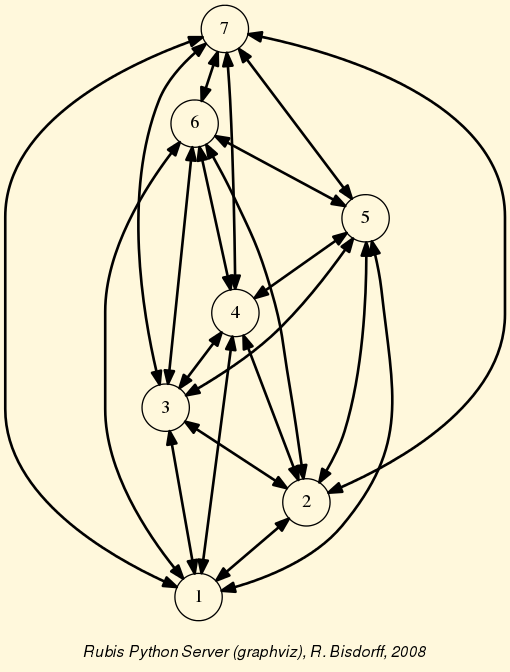
\includegraphics{strongComponents.png}\hfill}


\subsubsection{Strong components}
\label{tutorial:strong-components}\begin{description}
\item[{As the original digraph \emph{dg} was connected (see above the result of the \code{dg.showShort()} command), both the symmetric and transitive closures operated together, will necessarily produce a single strong commponent, i.e. a complete digraph. We may sometimes wish to collapse all strong components in a given digraph and construct the so reduced digraph. Using the \code{StrongComponentsCollapsedDigraph} constructor here will render a single hyper-node gathering all the original nodes :}] \leavevmode
\begin{Verbatim}[commandchars=\\\{\}]
\PYG{g+gp}{\PYGZgt{}\PYGZgt{}\PYGZgt{} }\PYG{k+kn}{from} \PYG{n+nn}{digraphs} \PYG{k+kn}{import} \PYG{n}{StrongComponentsCollapsedDigraph}
\PYG{g+gp}{\PYGZgt{}\PYGZgt{}\PYGZgt{} }\PYG{n}{sc} \PYG{o}{=} \PYG{n}{StrongComponentsCollapsedDigraph}\PYG{p}{(}\PYG{n}{dg}\PYG{p}{)}
\PYG{g+gp}{\PYGZgt{}\PYGZgt{}\PYGZgt{} }\PYG{n}{sc}\PYG{o}{.}\PYG{n}{showAll}\PYG{p}{(}\PYG{p}{)}
\PYG{g+go}{*\PYGZhy{}\PYGZhy{}\PYGZhy{}\PYGZhy{}\PYGZhy{} show detail \PYGZhy{}\PYGZhy{}\PYGZhy{}\PYGZhy{}\PYGZhy{}*}
\PYG{g+go}{Digraph          : tutRandValDigraph\PYGZus{}Scc}
\PYG{g+go}{*\PYGZhy{}\PYGZhy{}\PYGZhy{}\PYGZhy{} Actions \PYGZhy{}\PYGZhy{}\PYGZhy{}\PYGZhy{}*}
\PYG{g+go}{[\PYGZsq{}\PYGZus{}7\PYGZus{}1\PYGZus{}2\PYGZus{}6\PYGZus{}5\PYGZus{}3\PYGZus{}4\PYGZus{}\PYGZsq{}]}
\PYG{g+go}{* \PYGZhy{}\PYGZhy{}\PYGZhy{}\PYGZhy{} Relation Table \PYGZhy{}\PYGZhy{}\PYGZhy{}\PYGZhy{}\PYGZhy{}}
\PYG{g+go}{  S     \textbar{}  \PYGZsq{}Scc\PYGZus{}1\PYGZsq{}}
\PYG{g+go}{ \PYGZhy{}\PYGZhy{}\PYGZhy{}\PYGZhy{}\PYGZhy{}\PYGZhy{}\PYGZhy{}\textbar{}\PYGZhy{}\PYGZhy{}\PYGZhy{}\PYGZhy{}\PYGZhy{}\PYGZhy{}\PYGZhy{}\PYGZhy{}\PYGZhy{}}
\PYG{g+go}{\PYGZsq{}Scc\PYGZus{}1\PYGZsq{} \textbar{}  0.00}
\PYG{g+go}{short        content}
\PYG{g+go}{Scc\PYGZus{}1        \PYGZus{}7\PYGZus{}1\PYGZus{}2\PYGZus{}6\PYGZus{}5\PYGZus{}3\PYGZus{}4\PYGZus{}}
\PYG{g+go}{Neighborhoods:}
\PYG{g+go}{  Gamma     :}
\PYG{g+go}{\PYGZsq{}frozenset(\PYGZob{}\PYGZsq{}7\PYGZsq{}, \PYGZsq{}1\PYGZsq{}, \PYGZsq{}2\PYGZsq{}, \PYGZsq{}6\PYGZsq{}, \PYGZsq{}5\PYGZsq{}, \PYGZsq{}3\PYGZsq{}, \PYGZsq{}4\PYGZsq{}\PYGZcb{})\PYGZsq{}: in =\PYGZgt{} set(), out =\PYGZgt{} set()}
\PYG{g+go}{  Not Gamma :}
\PYG{g+go}{\PYGZsq{}frozenset(\PYGZob{}\PYGZsq{}7\PYGZsq{}, \PYGZsq{}1\PYGZsq{}, \PYGZsq{}2\PYGZsq{}, \PYGZsq{}6\PYGZsq{}, \PYGZsq{}5\PYGZsq{}, \PYGZsq{}3\PYGZsq{}, \PYGZsq{}4\PYGZsq{}\PYGZcb{})\PYGZsq{}: in =\PYGZgt{} set(), out =\PYGZgt{} set()}
\PYG{g+gp}{\PYGZgt{}\PYGZgt{}\PYGZgt{} }\PYG{o}{.}\PYG{o}{.}\PYG{o}{.}
\end{Verbatim}

\end{description}


\subsubsection{Saving and reloading in CSV format}
\label{tutorial:saving-and-reloading-in-csv-format}\begin{description}
\item[{Sometimes it is required to exchange the graph valuation data in CSV format with a statistical package like \href{http://www.r-project.org/}{R}. For this purpose it is possible to export the digraph data into a CSV file. The valuation domain is hereby normalized by default to the range {[}-1,1{]} and the diagonal put by defalut to the minimal value -1:}] \leavevmode
\begin{Verbatim}[commandchars=\\\{\}]
\PYG{g+gp}{\PYGZgt{}\PYGZgt{}\PYGZgt{} }\PYG{n}{dg} \PYG{o}{=} \PYG{n}{Digraph}\PYG{p}{(}\PYG{l+s}{\PYGZsq{}}\PYG{l+s}{tutRandValDigraph}\PYG{l+s}{\PYGZsq{}}\PYG{p}{)}
\PYG{g+gp}{\PYGZgt{}\PYGZgt{}\PYGZgt{} }\PYG{n}{dg}\PYG{o}{.}\PYG{n}{saveCSV}\PYG{p}{(}\PYG{l+s}{\PYGZsq{}}\PYG{l+s}{tutRandValDigraph}\PYG{l+s}{\PYGZsq{}}\PYG{p}{)}
\PYG{g+go}{\PYGZsh{} content of file tutRandValDigraph.csv}
\PYG{g+go}{\PYGZdq{}d\PYGZdq{},\PYGZdq{}1\PYGZdq{},\PYGZdq{}2\PYGZdq{},\PYGZdq{}3\PYGZdq{},\PYGZdq{}4\PYGZdq{},\PYGZdq{}5\PYGZdq{},\PYGZdq{}6\PYGZdq{},\PYGZdq{}7\PYGZdq{}}
\PYG{g+go}{\PYGZdq{}1\PYGZdq{},\PYGZhy{}1.0,0.48,\PYGZhy{}0.7,\PYGZhy{}0.86,\PYGZhy{}0.3,\PYGZhy{}0.38,\PYGZhy{}0.44}
\PYG{g+go}{\PYGZdq{}2\PYGZdq{},0.22,\PYGZhy{}1.0,0.38,\PYGZhy{}0.5,\PYGZhy{}0.8,0.54,\PYGZhy{}0.02}
\PYG{g+go}{\PYGZdq{}3\PYGZdq{},0.42,\PYGZhy{}0.08,\PYGZhy{}1.0,\PYGZhy{}0.7,0.56,\PYGZhy{}0.84,1.0}
\PYG{g+go}{\PYGZdq{}4\PYGZdq{},\PYGZhy{}0.44,0.4,0.62,\PYGZhy{}1.0,\PYGZhy{}0.04,\PYGZhy{}0.66,\PYGZhy{}0.76}
\PYG{g+go}{\PYGZdq{}5\PYGZdq{},\PYGZhy{}0.32,0.48,0.46,\PYGZhy{}0.64,\PYGZhy{}1.0,0.22,0.52}
\PYG{g+go}{\PYGZdq{}6\PYGZdq{},0.84,0.0,0.4,0.96,0.18,\PYGZhy{}1.0,0.22}
\PYG{g+go}{\PYGZdq{}7\PYGZdq{},\PYGZhy{}0.88,\PYGZhy{}0.72,\PYGZhy{}0.82,\PYGZhy{}0.52,0.84,\PYGZhy{}0.04,\PYGZhy{}1.0}
\end{Verbatim}

\item[{It is possible to reload a Digraph instance from its previously saved CSV file content:}] \leavevmode
\begin{Verbatim}[commandchars=\\\{\}]
\PYG{g+gp}{\PYGZgt{}\PYGZgt{}\PYGZgt{} }\PYG{n}{dgcsv} \PYG{o}{=} \PYG{n}{CSVDigraph}\PYG{p}{(}\PYG{l+s}{\PYGZsq{}}\PYG{l+s}{tutRandValDigraph}\PYG{l+s}{\PYGZsq{}}\PYG{p}{)}
\PYG{g+gp}{\PYGZgt{}\PYGZgt{}\PYGZgt{} }\PYG{n}{dgcsv}\PYG{o}{.}\PYG{n}{showRelationTable}\PYG{p}{(}\PYG{n}{ReflexiveTerms}\PYG{o}{=}\PYG{n+nb+bp}{False}\PYG{p}{)}
\PYG{g+go}{* \PYGZhy{}\PYGZhy{}\PYGZhy{}\PYGZhy{} Relation Table \PYGZhy{}\PYGZhy{}\PYGZhy{}\PYGZhy{}\PYGZhy{}}
\PYG{g+go}{r(xSy) \textbar{}   \PYGZsq{}1\PYGZsq{}   \PYGZsq{}2\PYGZsq{}   \PYGZsq{}3\PYGZsq{}   \PYGZsq{}4\PYGZsq{}   \PYGZsq{}5\PYGZsq{}   \PYGZsq{}6\PYGZsq{}   \PYGZsq{}7\PYGZsq{}}
\PYG{g+go}{\PYGZhy{}\PYGZhy{}\PYGZhy{}\PYGZhy{}\PYGZhy{}\PYGZhy{}\PYGZhy{}\textbar{}\PYGZhy{}\PYGZhy{}\PYGZhy{}\PYGZhy{}\PYGZhy{}\PYGZhy{}\PYGZhy{}\PYGZhy{}\PYGZhy{}\PYGZhy{}\PYGZhy{}\PYGZhy{}\PYGZhy{}\PYGZhy{}\PYGZhy{}\PYGZhy{}\PYGZhy{}\PYGZhy{}\PYGZhy{}\PYGZhy{}\PYGZhy{}\PYGZhy{}\PYGZhy{}\PYGZhy{}\PYGZhy{}\PYGZhy{}\PYGZhy{}\PYGZhy{}\PYGZhy{}\PYGZhy{}\PYGZhy{}\PYGZhy{}\PYGZhy{}\PYGZhy{}\PYGZhy{}\PYGZhy{}\PYGZhy{}\PYGZhy{}\PYGZhy{}\PYGZhy{}\PYGZhy{}\PYGZhy{}\PYGZhy{}\PYGZhy{}\PYGZhy{}\PYGZhy{}\PYGZhy{}\PYGZhy{}\PYGZhy{}\PYGZhy{}\PYGZhy{}\PYGZhy{}\PYGZhy{}\PYGZhy{}\PYGZhy{}\PYGZhy{}\PYGZhy{}\PYGZhy{}\PYGZhy{}\PYGZhy{}}
\PYG{g+go}{\PYGZsq{}1\PYGZsq{}    \textbar{}   \PYGZhy{}   \PYGZhy{}0.48  0.70  0.86  0.30  0.38  0.44}
\PYG{g+go}{\PYGZsq{}2\PYGZsq{}    \textbar{} \PYGZhy{}0.22   \PYGZhy{}   \PYGZhy{}0.38  0.50  0.80 \PYGZhy{}0.54  0.02}
\PYG{g+go}{\PYGZsq{}3\PYGZsq{}    \textbar{} \PYGZhy{}0.42  0.08   \PYGZhy{}    0.70 \PYGZhy{}0.56  0.84 \PYGZhy{}1.00}
\PYG{g+go}{\PYGZsq{}4\PYGZsq{}    \textbar{}  0.44 \PYGZhy{}0.40 \PYGZhy{}0.62   \PYGZhy{}    0.04  0.66  0.76}
\PYG{g+go}{\PYGZsq{}5\PYGZsq{}    \textbar{}  0.32 \PYGZhy{}0.48 \PYGZhy{}0.46  0.64   \PYGZhy{}   \PYGZhy{}0.22 \PYGZhy{}0.52}
\PYG{g+go}{\PYGZsq{}6\PYGZsq{}    \textbar{} \PYGZhy{}0.84  0.00 \PYGZhy{}0.40 \PYGZhy{}0.96 \PYGZhy{}0.18   \PYGZhy{}   \PYGZhy{}0.22}
\PYG{g+go}{\PYGZsq{}7\PYGZsq{}    \textbar{}  0.88  0.72  0.82  0.52 \PYGZhy{}0.84  0.04   \PYGZhy{}}
\end{Verbatim}

\end{description}


\subsubsection{Complete, empty and indeterminate digraphs}
\label{tutorial:complete-empty-and-indeterminate-digraphs}\begin{description}
\item[{Let us finally mention some special universal classes of digraphs that are readily available in the \code{digraphs} module, like the \code{CompleteDigraph}, the \code{EmptyDigraph} and the \code{IndeterminateDigraph} classes, which put all characteristic values respectively to the \emph{maximum}, the \emph{minimum} or the median \emph{indeterminate} characteristic value:}] \leavevmode
\begin{Verbatim}[commandchars=\\\{\}]
\PYG{g+gp}{\PYGZgt{}\PYGZgt{}\PYGZgt{} }\PYG{k+kn}{from} \PYG{n+nn}{diggraphs} \PYG{k+kn}{import} \PYG{n}{CompleteDigraph}\PYG{p}{,} \PYG{n}{EmptyDigraph}\PYG{p}{,} \PYG{n}{IndeterminateDigraph}
\PYG{g+gp}{\PYGZgt{}\PYGZgt{}\PYGZgt{} }\PYG{n}{help}\PYG{p}{(}\PYG{n}{CompleteDigraph}\PYG{p}{)}
\PYG{g+go}{Help on class CompleteDigraph in module digraphs:}
\PYG{g+go}{class CompleteDigraph(Digraph)}
\PYG{g+go}{ \textbar{}  Parameters:}
\PYG{g+go}{ \textbar{}      order \PYGZgt{} 0; valuationdomain=(Min,Max).}
\PYG{g+go}{ \textbar{}  Specialization of the general Digraph class for generating}
\PYG{g+go}{ \textbar{}  temporary complete graphs of order 5 in \PYGZob{}\PYGZhy{}1,0,1\PYGZcb{} by default.}
\PYG{g+go}{ \textbar{}  Method resolution order:}
\PYG{g+go}{ \textbar{}      CompleteDigraph}
\PYG{g+go}{ \textbar{}      Digraph}
\PYG{g+go}{ \textbar{}      builtins.object}
\PYG{g+gp}{...}
\PYG{g+gp}{\PYGZgt{}\PYGZgt{}\PYGZgt{} }\PYG{n}{e} \PYG{o}{=} \PYG{n}{EmptyDigraph}\PYG{p}{(}\PYG{n}{order}\PYG{o}{=}\PYG{l+m+mi}{5}\PYG{p}{)}
\PYG{g+gp}{\PYGZgt{}\PYGZgt{}\PYGZgt{} }\PYG{n}{e}\PYG{o}{.}\PYG{n}{showRelationTable}\PYG{p}{(}\PYG{p}{)}
\PYG{g+go}{* \PYGZhy{}\PYGZhy{}\PYGZhy{}\PYGZhy{} Relation Table \PYGZhy{}\PYGZhy{}\PYGZhy{}\PYGZhy{}\PYGZhy{}}
\PYG{g+go}{  S   \textbar{}  \PYGZsq{}1\PYGZsq{}      \PYGZsq{}2\PYGZsq{}     \PYGZsq{}3\PYGZsq{}     \PYGZsq{}4\PYGZsq{}     \PYGZsq{}5\PYGZsq{}}
\PYG{g+go}{\PYGZhy{}\PYGZhy{}\PYGZhy{}\PYGZhy{} \PYGZhy{}\textbar{}\PYGZhy{}\PYGZhy{}\PYGZhy{}\PYGZhy{}\PYGZhy{}\PYGZhy{}\PYGZhy{}\PYGZhy{}\PYGZhy{}\PYGZhy{}\PYGZhy{}\PYGZhy{}\PYGZhy{}\PYGZhy{}\PYGZhy{}\PYGZhy{}\PYGZhy{}\PYGZhy{}\PYGZhy{}\PYGZhy{}\PYGZhy{}\PYGZhy{}\PYGZhy{}\PYGZhy{}\PYGZhy{}\PYGZhy{}\PYGZhy{}\PYGZhy{}\PYGZhy{}\PYGZhy{}\PYGZhy{}\PYGZhy{}\PYGZhy{}\PYGZhy{}\PYGZhy{}\PYGZhy{}\PYGZhy{}\PYGZhy{}\PYGZhy{}}
\PYG{g+go}{\PYGZsq{}1\PYGZsq{}   \textbar{}  \PYGZhy{}1.00   \PYGZhy{}1.00   \PYGZhy{}1.00   \PYGZhy{}1.00   \PYGZhy{}1.00}
\PYG{g+go}{\PYGZsq{}2\PYGZsq{}   \textbar{}  \PYGZhy{}1.00   \PYGZhy{}1.00   \PYGZhy{}1.00   \PYGZhy{}1.00   \PYGZhy{}1.00}
\PYG{g+go}{\PYGZsq{}3\PYGZsq{}   \textbar{}  \PYGZhy{}1.00   \PYGZhy{}1.00   \PYGZhy{}1.00   \PYGZhy{}1.00   \PYGZhy{}1.00}
\PYG{g+go}{\PYGZsq{}4\PYGZsq{}   \textbar{}  \PYGZhy{}1.00   \PYGZhy{}1.00   \PYGZhy{}1.00   \PYGZhy{}1.00   \PYGZhy{}1.00}
\PYG{g+go}{\PYGZsq{}5\PYGZsq{}   \textbar{}  \PYGZhy{}1.00   \PYGZhy{}1.00   \PYGZhy{}1.00   \PYGZhy{}1.00   \PYGZhy{}1.00}
\PYG{g+gp}{\PYGZgt{}\PYGZgt{}\PYGZgt{} }\PYG{n}{e}\PYG{o}{.}\PYG{n}{showNeighborhoods}\PYG{p}{(}\PYG{p}{)}
\PYG{g+go}{Neighborhoods:}
\PYG{g+go}{  Gamma     :}
\PYG{g+go}{\PYGZsq{}1\PYGZsq{}: in =\PYGZgt{} set(), out =\PYGZgt{} set()}
\PYG{g+go}{\PYGZsq{}2\PYGZsq{}: in =\PYGZgt{} set(), out =\PYGZgt{} set()}
\PYG{g+go}{\PYGZsq{}5\PYGZsq{}: in =\PYGZgt{} set(), out =\PYGZgt{} set()}
\PYG{g+go}{\PYGZsq{}3\PYGZsq{}: in =\PYGZgt{} set(), out =\PYGZgt{} set()}
\PYG{g+go}{\PYGZsq{}4\PYGZsq{}: in =\PYGZgt{} set(), out =\PYGZgt{} set()}
\PYG{g+go}{  Not Gamma :}
\PYG{g+go}{\PYGZsq{}1\PYGZsq{}: in =\PYGZgt{} \PYGZob{}\PYGZsq{}2\PYGZsq{}, \PYGZsq{}4\PYGZsq{}, \PYGZsq{}5\PYGZsq{}, \PYGZsq{}3\PYGZsq{}\PYGZcb{}, out =\PYGZgt{} \PYGZob{}\PYGZsq{}2\PYGZsq{}, \PYGZsq{}4\PYGZsq{}, \PYGZsq{}5\PYGZsq{}, \PYGZsq{}3\PYGZsq{}\PYGZcb{}}
\PYG{g+go}{\PYGZsq{}2\PYGZsq{}: in =\PYGZgt{} \PYGZob{}\PYGZsq{}1\PYGZsq{}, \PYGZsq{}4\PYGZsq{}, \PYGZsq{}5\PYGZsq{}, \PYGZsq{}3\PYGZsq{}\PYGZcb{}, out =\PYGZgt{} \PYGZob{}\PYGZsq{}1\PYGZsq{}, \PYGZsq{}4\PYGZsq{}, \PYGZsq{}5\PYGZsq{}, \PYGZsq{}3\PYGZsq{}\PYGZcb{}}
\PYG{g+go}{\PYGZsq{}5\PYGZsq{}: in =\PYGZgt{} \PYGZob{}\PYGZsq{}1\PYGZsq{}, \PYGZsq{}2\PYGZsq{}, \PYGZsq{}4\PYGZsq{}, \PYGZsq{}3\PYGZsq{}\PYGZcb{}, out =\PYGZgt{} \PYGZob{}\PYGZsq{}1\PYGZsq{}, \PYGZsq{}2\PYGZsq{}, \PYGZsq{}4\PYGZsq{}, \PYGZsq{}3\PYGZsq{}\PYGZcb{}}
\PYG{g+go}{\PYGZsq{}3\PYGZsq{}: in =\PYGZgt{} \PYGZob{}\PYGZsq{}1\PYGZsq{}, \PYGZsq{}2\PYGZsq{}, \PYGZsq{}4\PYGZsq{}, \PYGZsq{}5\PYGZsq{}\PYGZcb{}, out =\PYGZgt{} \PYGZob{}\PYGZsq{}1\PYGZsq{}, \PYGZsq{}2\PYGZsq{}, \PYGZsq{}4\PYGZsq{}, \PYGZsq{}5\PYGZsq{}\PYGZcb{}}
\PYG{g+go}{\PYGZsq{}4\PYGZsq{}: in =\PYGZgt{} \PYGZob{}\PYGZsq{}1\PYGZsq{}, \PYGZsq{}2\PYGZsq{}, \PYGZsq{}5\PYGZsq{}, \PYGZsq{}3\PYGZsq{}\PYGZcb{}, out =\PYGZgt{} \PYGZob{}\PYGZsq{}1\PYGZsq{}, \PYGZsq{}2\PYGZsq{}, \PYGZsq{}5\PYGZsq{}, \PYGZsq{}3\PYGZsq{}\PYGZcb{}}
\PYG{g+gp}{\PYGZgt{}\PYGZgt{}\PYGZgt{} }\PYG{n}{i} \PYG{o}{=} \PYG{n}{IndeterminateDigraph}\PYG{p}{(}\PYG{p}{)}
\PYG{g+go}{* \PYGZhy{}\PYGZhy{}\PYGZhy{}\PYGZhy{} Relation Table \PYGZhy{}\PYGZhy{}\PYGZhy{}\PYGZhy{}\PYGZhy{}}
\PYG{g+go}{  S   \textbar{}  \PYGZsq{}1\PYGZsq{}      \PYGZsq{}2\PYGZsq{}     \PYGZsq{}3\PYGZsq{}     \PYGZsq{}4\PYGZsq{}     \PYGZsq{}5\PYGZsq{}}
\PYG{g+go}{\PYGZhy{}\PYGZhy{}\PYGZhy{}\PYGZhy{}\PYGZhy{}\PYGZhy{}\textbar{}\PYGZhy{}\PYGZhy{}\PYGZhy{}\PYGZhy{}\PYGZhy{}\PYGZhy{}\PYGZhy{}\PYGZhy{}\PYGZhy{}\PYGZhy{}\PYGZhy{}\PYGZhy{}\PYGZhy{}\PYGZhy{}\PYGZhy{}\PYGZhy{}\PYGZhy{}\PYGZhy{}\PYGZhy{}\PYGZhy{}\PYGZhy{}\PYGZhy{}\PYGZhy{}\PYGZhy{}\PYGZhy{}\PYGZhy{}\PYGZhy{}\PYGZhy{}\PYGZhy{}\PYGZhy{}\PYGZhy{}\PYGZhy{}\PYGZhy{}\PYGZhy{}\PYGZhy{}\PYGZhy{}\PYGZhy{}\PYGZhy{}}
\PYG{g+go}{\PYGZsq{}1\PYGZsq{}   \textbar{}  0.00    0.00    0.00    0.00    0.00}
\PYG{g+go}{\PYGZsq{}2\PYGZsq{}   \textbar{}  0.00    0.00    0.00    0.00    0.00}
\PYG{g+go}{\PYGZsq{}3\PYGZsq{}   \textbar{}  0.00    0.00    0.00    0.00    0.00}
\PYG{g+go}{\PYGZsq{}4\PYGZsq{}   \textbar{}  0.00    0.00    0.00    0.00    0.00}
\PYG{g+go}{\PYGZsq{}5\PYGZsq{}   \textbar{}  0.00    0.00    0.00    0.00    0.00}
\PYG{g+gp}{\PYGZgt{}\PYGZgt{}\PYGZgt{} }\PYG{n}{i}\PYG{o}{.}\PYG{n}{showNeighborhoods}\PYG{p}{(}\PYG{p}{)}
\PYG{g+go}{Neighborhoods:}
\PYG{g+go}{  Gamma     :}
\PYG{g+go}{\PYGZsq{}1\PYGZsq{}: in =\PYGZgt{} set(), out =\PYGZgt{} set()}
\PYG{g+go}{\PYGZsq{}2\PYGZsq{}: in =\PYGZgt{} set(), out =\PYGZgt{} set()}
\PYG{g+go}{\PYGZsq{}5\PYGZsq{}: in =\PYGZgt{} set(), out =\PYGZgt{} set()}
\PYG{g+go}{\PYGZsq{}3\PYGZsq{}: in =\PYGZgt{} set(), out =\PYGZgt{} set()}
\PYG{g+go}{\PYGZsq{}4\PYGZsq{}: in =\PYGZgt{} set(), out =\PYGZgt{} set()}
\PYG{g+go}{  Not Gamma :}
\PYG{g+go}{\PYGZsq{}1\PYGZsq{}: in =\PYGZgt{} set(), out =\PYGZgt{} set()}
\PYG{g+go}{\PYGZsq{}2\PYGZsq{}: in =\PYGZgt{} set(), out =\PYGZgt{} set()}
\PYG{g+go}{\PYGZsq{}5\PYGZsq{}: in =\PYGZgt{} set(), out =\PYGZgt{} set()}
\PYG{g+go}{\PYGZsq{}3\PYGZsq{}: in =\PYGZgt{} set(), out =\PYGZgt{} set()}
\PYG{g+go}{\PYGZsq{}4\PYGZsq{}: in =\PYGZgt{} set(), out =\PYGZgt{} set()}
\end{Verbatim}

\end{description}

\begin{notice}{note}{Note:}
Notice the subtle difference between the neighborhoods of an \emph{empty} and the neighborhoods of an \emph{indeterminate} digraph instance. In the first kind, the neighborhoods are known to be completely \emph{empty} whereas, in the latter, \emph{nothing is known} about the actual neighborhoods of the nodes. These two cases illustrate why in the case of a bipolar valuation domain, we need both a \emph{gamma} \textbf{and} a \emph{notGamma} function.
\end{notice}

Back to {\hyperref[tutorial:tutorial-label]{\emph{Content}}}


\subsection{Working with the \texttt{graphs} module}
\label{tutorial:working-with-the-graphs-module}\label{tutorial:graphs-tutorial-label}

\subsubsection{Structure of a \texttt{Graph} object}
\label{tutorial:structure-of-a-graph-object}
In the \code{graphs} module, the root \code{Graph} class provides a generic \textbf{simple graph model}, without loops and multiple links. A given object of this class consists in:
\begin{enumerate}
\item {} 
the graph \textbf{vertices} : a dictionary of vertices with `name' and `shortname' attributes,

\item {} 
the graph \textbf{valuationDomain} , a dictionary with three entries: the minimum (-1, means certainly no link), the median (0, means missing information) and the maximum characteristic value (+1, means certainly a link),

\item {} 
the graph \textbf{edges} : a dictionary with frozensets of pairs of vertices as entries carrying a characteristic value in the range of the previous valuation domain,

\item {} 
and its associated \textbf{gamma function} : a dictionary containing the direct neighbors of each vertice, automatically added by the object constructor.

\end{enumerate}

See the technical documentation of the {\hyperref[techDoc:graphs-label]{\emph{graphs module}}}.
\begin{description}
\item[{Example Python3 session:}] \leavevmode
\begin{Verbatim}[commandchars=\\\{\}]
\PYG{g+gp}{\PYGZgt{}\PYGZgt{}\PYGZgt{} }\PYG{k+kn}{from} \PYG{n+nn}{graphs} \PYG{k+kn}{import} \PYG{n}{Graph}
\PYG{g+gp}{\PYGZgt{}\PYGZgt{}\PYGZgt{} }\PYG{n}{g} \PYG{o}{=} \PYG{n}{Graph}\PYG{p}{(}\PYG{n}{numberOfVertices}\PYG{o}{=}\PYG{l+m+mi}{7}\PYG{p}{,}\PYG{n}{edgeProbability}\PYG{o}{=}\PYG{l+m+mf}{0.5}\PYG{p}{)}
\PYG{g+gp}{\PYGZgt{}\PYGZgt{}\PYGZgt{} }\PYG{n}{g}\PYG{o}{.}\PYG{n}{showShort}\PYG{p}{(}\PYG{p}{)}
\PYG{g+go}{*\PYGZhy{}\PYGZhy{}\PYGZhy{}\PYGZhy{}\PYGZhy{} show short \PYGZhy{}\PYGZhy{}\PYGZhy{}\PYGZhy{}\PYGZhy{}\PYGZhy{}\PYGZhy{}\PYGZhy{}\PYGZhy{}\PYGZhy{}\PYGZhy{}\PYGZhy{}\PYGZhy{}\PYGZhy{}*}
\PYG{g+go}{Name             : \PYGZsq{}randomGraph\PYGZsq{}}
\PYG{g+go}{Vertices         :  [\PYGZsq{}v1\PYGZsq{}, \PYGZsq{}v2\PYGZsq{}, \PYGZsq{}v3\PYGZsq{}, \PYGZsq{}v4\PYGZsq{}, \PYGZsq{}v5\PYGZsq{}, \PYGZsq{}v6\PYGZsq{}, \PYGZsq{}v7\PYGZsq{}]}
\PYG{g+go}{Valuation domain :  \PYGZob{}\PYGZsq{}med\PYGZsq{}: 0, \PYGZsq{}max\PYGZsq{}: 1, \PYGZsq{}min\PYGZsq{}: \PYGZhy{}1\PYGZcb{}}
\PYG{g+go}{Gamma function   :}
\PYG{g+go}{v1 \PYGZhy{}\PYGZgt{} [\PYGZsq{}v5\PYGZsq{}]}
\PYG{g+go}{v2 \PYGZhy{}\PYGZgt{} [\PYGZsq{}v4\PYGZsq{}, \PYGZsq{}v6\PYGZsq{}, \PYGZsq{}v3\PYGZsq{}]}
\PYG{g+go}{v3 \PYGZhy{}\PYGZgt{} [\PYGZsq{}v2\PYGZsq{}]}
\PYG{g+go}{v4 \PYGZhy{}\PYGZgt{} [\PYGZsq{}v5\PYGZsq{}, \PYGZsq{}v2\PYGZsq{}, \PYGZsq{}v7\PYGZsq{}]}
\PYG{g+go}{v5 \PYGZhy{}\PYGZgt{} [\PYGZsq{}v4\PYGZsq{}, \PYGZsq{}v6\PYGZsq{}, \PYGZsq{}v1\PYGZsq{}]}
\PYG{g+go}{v6 \PYGZhy{}\PYGZgt{} [\PYGZsq{}v5\PYGZsq{}, \PYGZsq{}v2\PYGZsq{}]}
\PYG{g+go}{v7 \PYGZhy{}\PYGZgt{} [\PYGZsq{}v4\PYGZsq{}]}
\PYG{g+gp}{\PYGZgt{}\PYGZgt{}\PYGZgt{} }\PYG{n}{g}\PYG{o}{.}\PYG{n}{save}\PYG{p}{(}\PYG{n}{fileName}\PYG{o}{=}\PYG{l+s}{\PYGZsq{}}\PYG{l+s}{tutorialGraph}\PYG{l+s}{\PYGZsq{}}\PYG{p}{)}
\end{Verbatim}

\end{description}

The saved Graph instance named \code{tutorialGraph.py} is encoded in python3 as follows:

\begin{Verbatim}[commandchars=\\\{\}]
\PYG{c}{\PYGZsh{} Graph instance saved in Python format}
\PYG{n}{vertices} \PYG{o}{=} \PYG{p}{\PYGZob{}}
\PYG{l+s}{\PYGZsq{}}\PYG{l+s}{v1}\PYG{l+s}{\PYGZsq{}}\PYG{p}{:} \PYG{p}{\PYGZob{}}\PYG{l+s}{\PYGZsq{}}\PYG{l+s}{shortName}\PYG{l+s}{\PYGZsq{}}\PYG{p}{:} \PYG{l+s}{\PYGZsq{}}\PYG{l+s}{v1}\PYG{l+s}{\PYGZsq{}}\PYG{p}{,} \PYG{l+s}{\PYGZsq{}}\PYG{l+s}{name}\PYG{l+s}{\PYGZsq{}}\PYG{p}{:} \PYG{l+s}{\PYGZsq{}}\PYG{l+s}{random vertex}\PYG{l+s}{\PYGZsq{}}\PYG{p}{\PYGZcb{}}\PYG{p}{,}
\PYG{l+s}{\PYGZsq{}}\PYG{l+s}{v2}\PYG{l+s}{\PYGZsq{}}\PYG{p}{:} \PYG{p}{\PYGZob{}}\PYG{l+s}{\PYGZsq{}}\PYG{l+s}{shortName}\PYG{l+s}{\PYGZsq{}}\PYG{p}{:} \PYG{l+s}{\PYGZsq{}}\PYG{l+s}{v2}\PYG{l+s}{\PYGZsq{}}\PYG{p}{,} \PYG{l+s}{\PYGZsq{}}\PYG{l+s}{name}\PYG{l+s}{\PYGZsq{}}\PYG{p}{:} \PYG{l+s}{\PYGZsq{}}\PYG{l+s}{random vertex}\PYG{l+s}{\PYGZsq{}}\PYG{p}{\PYGZcb{}}\PYG{p}{,}
\PYG{l+s}{\PYGZsq{}}\PYG{l+s}{v3}\PYG{l+s}{\PYGZsq{}}\PYG{p}{:} \PYG{p}{\PYGZob{}}\PYG{l+s}{\PYGZsq{}}\PYG{l+s}{shortName}\PYG{l+s}{\PYGZsq{}}\PYG{p}{:} \PYG{l+s}{\PYGZsq{}}\PYG{l+s}{v3}\PYG{l+s}{\PYGZsq{}}\PYG{p}{,} \PYG{l+s}{\PYGZsq{}}\PYG{l+s}{name}\PYG{l+s}{\PYGZsq{}}\PYG{p}{:} \PYG{l+s}{\PYGZsq{}}\PYG{l+s}{random vertex}\PYG{l+s}{\PYGZsq{}}\PYG{p}{\PYGZcb{}}\PYG{p}{,}
\PYG{l+s}{\PYGZsq{}}\PYG{l+s}{v4}\PYG{l+s}{\PYGZsq{}}\PYG{p}{:} \PYG{p}{\PYGZob{}}\PYG{l+s}{\PYGZsq{}}\PYG{l+s}{shortName}\PYG{l+s}{\PYGZsq{}}\PYG{p}{:} \PYG{l+s}{\PYGZsq{}}\PYG{l+s}{v4}\PYG{l+s}{\PYGZsq{}}\PYG{p}{,} \PYG{l+s}{\PYGZsq{}}\PYG{l+s}{name}\PYG{l+s}{\PYGZsq{}}\PYG{p}{:} \PYG{l+s}{\PYGZsq{}}\PYG{l+s}{random vertex}\PYG{l+s}{\PYGZsq{}}\PYG{p}{\PYGZcb{}}\PYG{p}{,}
\PYG{l+s}{\PYGZsq{}}\PYG{l+s}{v5}\PYG{l+s}{\PYGZsq{}}\PYG{p}{:} \PYG{p}{\PYGZob{}}\PYG{l+s}{\PYGZsq{}}\PYG{l+s}{shortName}\PYG{l+s}{\PYGZsq{}}\PYG{p}{:} \PYG{l+s}{\PYGZsq{}}\PYG{l+s}{v5}\PYG{l+s}{\PYGZsq{}}\PYG{p}{,} \PYG{l+s}{\PYGZsq{}}\PYG{l+s}{name}\PYG{l+s}{\PYGZsq{}}\PYG{p}{:} \PYG{l+s}{\PYGZsq{}}\PYG{l+s}{random vertex}\PYG{l+s}{\PYGZsq{}}\PYG{p}{\PYGZcb{}}\PYG{p}{,}
\PYG{l+s}{\PYGZsq{}}\PYG{l+s}{v6}\PYG{l+s}{\PYGZsq{}}\PYG{p}{:} \PYG{p}{\PYGZob{}}\PYG{l+s}{\PYGZsq{}}\PYG{l+s}{shortName}\PYG{l+s}{\PYGZsq{}}\PYG{p}{:} \PYG{l+s}{\PYGZsq{}}\PYG{l+s}{v6}\PYG{l+s}{\PYGZsq{}}\PYG{p}{,} \PYG{l+s}{\PYGZsq{}}\PYG{l+s}{name}\PYG{l+s}{\PYGZsq{}}\PYG{p}{:} \PYG{l+s}{\PYGZsq{}}\PYG{l+s}{random vertex}\PYG{l+s}{\PYGZsq{}}\PYG{p}{\PYGZcb{}}\PYG{p}{,}
\PYG{l+s}{\PYGZsq{}}\PYG{l+s}{v7}\PYG{l+s}{\PYGZsq{}}\PYG{p}{:} \PYG{p}{\PYGZob{}}\PYG{l+s}{\PYGZsq{}}\PYG{l+s}{shortName}\PYG{l+s}{\PYGZsq{}}\PYG{p}{:} \PYG{l+s}{\PYGZsq{}}\PYG{l+s}{v7}\PYG{l+s}{\PYGZsq{}}\PYG{p}{,} \PYG{l+s}{\PYGZsq{}}\PYG{l+s}{name}\PYG{l+s}{\PYGZsq{}}\PYG{p}{:} \PYG{l+s}{\PYGZsq{}}\PYG{l+s}{random vertex}\PYG{l+s}{\PYGZsq{}}\PYG{p}{\PYGZcb{}}\PYG{p}{,}
\PYG{p}{\PYGZcb{}}
\PYG{n}{valuationDomain} \PYG{o}{=} \PYG{p}{\PYGZob{}}\PYG{l+s}{\PYGZsq{}}\PYG{l+s}{min}\PYG{l+s}{\PYGZsq{}}\PYG{p}{:}\PYG{o}{\PYGZhy{}}\PYG{l+m+mi}{1}\PYG{p}{,}\PYG{l+s}{\PYGZsq{}}\PYG{l+s}{med}\PYG{l+s}{\PYGZsq{}}\PYG{p}{:}\PYG{l+m+mi}{0}\PYG{p}{,}\PYG{l+s}{\PYGZsq{}}\PYG{l+s}{max}\PYG{l+s}{\PYGZsq{}}\PYG{p}{:}\PYG{l+m+mi}{1}\PYG{p}{\PYGZcb{}}
\PYG{n}{edges} \PYG{o}{=} \PYG{p}{\PYGZob{}}
\PYG{n+nb}{frozenset}\PYG{p}{(}\PYG{p}{[}\PYG{l+s}{\PYGZsq{}}\PYG{l+s}{v1}\PYG{l+s}{\PYGZsq{}}\PYG{p}{,}\PYG{l+s}{\PYGZsq{}}\PYG{l+s}{v2}\PYG{l+s}{\PYGZsq{}}\PYG{p}{]}\PYG{p}{)} \PYG{p}{:} \PYG{o}{\PYGZhy{}}\PYG{l+m+mi}{1}\PYG{p}{,}
\PYG{n+nb}{frozenset}\PYG{p}{(}\PYG{p}{[}\PYG{l+s}{\PYGZsq{}}\PYG{l+s}{v1}\PYG{l+s}{\PYGZsq{}}\PYG{p}{,}\PYG{l+s}{\PYGZsq{}}\PYG{l+s}{v3}\PYG{l+s}{\PYGZsq{}}\PYG{p}{]}\PYG{p}{)} \PYG{p}{:} \PYG{o}{\PYGZhy{}}\PYG{l+m+mi}{1}\PYG{p}{,}
\PYG{n+nb}{frozenset}\PYG{p}{(}\PYG{p}{[}\PYG{l+s}{\PYGZsq{}}\PYG{l+s}{v1}\PYG{l+s}{\PYGZsq{}}\PYG{p}{,}\PYG{l+s}{\PYGZsq{}}\PYG{l+s}{v4}\PYG{l+s}{\PYGZsq{}}\PYG{p}{]}\PYG{p}{)} \PYG{p}{:} \PYG{o}{\PYGZhy{}}\PYG{l+m+mi}{1}\PYG{p}{,}
\PYG{n+nb}{frozenset}\PYG{p}{(}\PYG{p}{[}\PYG{l+s}{\PYGZsq{}}\PYG{l+s}{v1}\PYG{l+s}{\PYGZsq{}}\PYG{p}{,}\PYG{l+s}{\PYGZsq{}}\PYG{l+s}{v5}\PYG{l+s}{\PYGZsq{}}\PYG{p}{]}\PYG{p}{)} \PYG{p}{:} \PYG{l+m+mi}{1}\PYG{p}{,}
\PYG{n+nb}{frozenset}\PYG{p}{(}\PYG{p}{[}\PYG{l+s}{\PYGZsq{}}\PYG{l+s}{v1}\PYG{l+s}{\PYGZsq{}}\PYG{p}{,}\PYG{l+s}{\PYGZsq{}}\PYG{l+s}{v6}\PYG{l+s}{\PYGZsq{}}\PYG{p}{]}\PYG{p}{)} \PYG{p}{:} \PYG{o}{\PYGZhy{}}\PYG{l+m+mi}{1}\PYG{p}{,}
\PYG{n+nb}{frozenset}\PYG{p}{(}\PYG{p}{[}\PYG{l+s}{\PYGZsq{}}\PYG{l+s}{v1}\PYG{l+s}{\PYGZsq{}}\PYG{p}{,}\PYG{l+s}{\PYGZsq{}}\PYG{l+s}{v7}\PYG{l+s}{\PYGZsq{}}\PYG{p}{]}\PYG{p}{)} \PYG{p}{:} \PYG{o}{\PYGZhy{}}\PYG{l+m+mi}{1}\PYG{p}{,}
\PYG{n+nb}{frozenset}\PYG{p}{(}\PYG{p}{[}\PYG{l+s}{\PYGZsq{}}\PYG{l+s}{v2}\PYG{l+s}{\PYGZsq{}}\PYG{p}{,}\PYG{l+s}{\PYGZsq{}}\PYG{l+s}{v3}\PYG{l+s}{\PYGZsq{}}\PYG{p}{]}\PYG{p}{)} \PYG{p}{:} \PYG{l+m+mi}{1}\PYG{p}{,}
\PYG{n+nb}{frozenset}\PYG{p}{(}\PYG{p}{[}\PYG{l+s}{\PYGZsq{}}\PYG{l+s}{v2}\PYG{l+s}{\PYGZsq{}}\PYG{p}{,}\PYG{l+s}{\PYGZsq{}}\PYG{l+s}{v4}\PYG{l+s}{\PYGZsq{}}\PYG{p}{]}\PYG{p}{)} \PYG{p}{:} \PYG{l+m+mi}{1}\PYG{p}{,}
\PYG{n+nb}{frozenset}\PYG{p}{(}\PYG{p}{[}\PYG{l+s}{\PYGZsq{}}\PYG{l+s}{v2}\PYG{l+s}{\PYGZsq{}}\PYG{p}{,}\PYG{l+s}{\PYGZsq{}}\PYG{l+s}{v5}\PYG{l+s}{\PYGZsq{}}\PYG{p}{]}\PYG{p}{)} \PYG{p}{:} \PYG{o}{\PYGZhy{}}\PYG{l+m+mi}{1}\PYG{p}{,}
\PYG{n+nb}{frozenset}\PYG{p}{(}\PYG{p}{[}\PYG{l+s}{\PYGZsq{}}\PYG{l+s}{v2}\PYG{l+s}{\PYGZsq{}}\PYG{p}{,}\PYG{l+s}{\PYGZsq{}}\PYG{l+s}{v6}\PYG{l+s}{\PYGZsq{}}\PYG{p}{]}\PYG{p}{)} \PYG{p}{:} \PYG{l+m+mi}{1}\PYG{p}{,}
\PYG{n+nb}{frozenset}\PYG{p}{(}\PYG{p}{[}\PYG{l+s}{\PYGZsq{}}\PYG{l+s}{v2}\PYG{l+s}{\PYGZsq{}}\PYG{p}{,}\PYG{l+s}{\PYGZsq{}}\PYG{l+s}{v7}\PYG{l+s}{\PYGZsq{}}\PYG{p}{]}\PYG{p}{)} \PYG{p}{:} \PYG{o}{\PYGZhy{}}\PYG{l+m+mi}{1}\PYG{p}{,}
\PYG{n+nb}{frozenset}\PYG{p}{(}\PYG{p}{[}\PYG{l+s}{\PYGZsq{}}\PYG{l+s}{v3}\PYG{l+s}{\PYGZsq{}}\PYG{p}{,}\PYG{l+s}{\PYGZsq{}}\PYG{l+s}{v4}\PYG{l+s}{\PYGZsq{}}\PYG{p}{]}\PYG{p}{)} \PYG{p}{:} \PYG{o}{\PYGZhy{}}\PYG{l+m+mi}{1}\PYG{p}{,}
\PYG{n+nb}{frozenset}\PYG{p}{(}\PYG{p}{[}\PYG{l+s}{\PYGZsq{}}\PYG{l+s}{v3}\PYG{l+s}{\PYGZsq{}}\PYG{p}{,}\PYG{l+s}{\PYGZsq{}}\PYG{l+s}{v5}\PYG{l+s}{\PYGZsq{}}\PYG{p}{]}\PYG{p}{)} \PYG{p}{:} \PYG{o}{\PYGZhy{}}\PYG{l+m+mi}{1}\PYG{p}{,}
\PYG{n+nb}{frozenset}\PYG{p}{(}\PYG{p}{[}\PYG{l+s}{\PYGZsq{}}\PYG{l+s}{v3}\PYG{l+s}{\PYGZsq{}}\PYG{p}{,}\PYG{l+s}{\PYGZsq{}}\PYG{l+s}{v6}\PYG{l+s}{\PYGZsq{}}\PYG{p}{]}\PYG{p}{)} \PYG{p}{:} \PYG{o}{\PYGZhy{}}\PYG{l+m+mi}{1}\PYG{p}{,}
\PYG{n+nb}{frozenset}\PYG{p}{(}\PYG{p}{[}\PYG{l+s}{\PYGZsq{}}\PYG{l+s}{v3}\PYG{l+s}{\PYGZsq{}}\PYG{p}{,}\PYG{l+s}{\PYGZsq{}}\PYG{l+s}{v7}\PYG{l+s}{\PYGZsq{}}\PYG{p}{]}\PYG{p}{)} \PYG{p}{:} \PYG{o}{\PYGZhy{}}\PYG{l+m+mi}{1}\PYG{p}{,}
\PYG{n+nb}{frozenset}\PYG{p}{(}\PYG{p}{[}\PYG{l+s}{\PYGZsq{}}\PYG{l+s}{v4}\PYG{l+s}{\PYGZsq{}}\PYG{p}{,}\PYG{l+s}{\PYGZsq{}}\PYG{l+s}{v5}\PYG{l+s}{\PYGZsq{}}\PYG{p}{]}\PYG{p}{)} \PYG{p}{:} \PYG{l+m+mi}{1}\PYG{p}{,}
\PYG{n+nb}{frozenset}\PYG{p}{(}\PYG{p}{[}\PYG{l+s}{\PYGZsq{}}\PYG{l+s}{v4}\PYG{l+s}{\PYGZsq{}}\PYG{p}{,}\PYG{l+s}{\PYGZsq{}}\PYG{l+s}{v6}\PYG{l+s}{\PYGZsq{}}\PYG{p}{]}\PYG{p}{)} \PYG{p}{:} \PYG{o}{\PYGZhy{}}\PYG{l+m+mi}{1}\PYG{p}{,}
\PYG{n+nb}{frozenset}\PYG{p}{(}\PYG{p}{[}\PYG{l+s}{\PYGZsq{}}\PYG{l+s}{v4}\PYG{l+s}{\PYGZsq{}}\PYG{p}{,}\PYG{l+s}{\PYGZsq{}}\PYG{l+s}{v7}\PYG{l+s}{\PYGZsq{}}\PYG{p}{]}\PYG{p}{)} \PYG{p}{:} \PYG{l+m+mi}{1}\PYG{p}{,}
\PYG{n+nb}{frozenset}\PYG{p}{(}\PYG{p}{[}\PYG{l+s}{\PYGZsq{}}\PYG{l+s}{v5}\PYG{l+s}{\PYGZsq{}}\PYG{p}{,}\PYG{l+s}{\PYGZsq{}}\PYG{l+s}{v6}\PYG{l+s}{\PYGZsq{}}\PYG{p}{]}\PYG{p}{)} \PYG{p}{:} \PYG{l+m+mi}{1}\PYG{p}{,}
\PYG{n+nb}{frozenset}\PYG{p}{(}\PYG{p}{[}\PYG{l+s}{\PYGZsq{}}\PYG{l+s}{v5}\PYG{l+s}{\PYGZsq{}}\PYG{p}{,}\PYG{l+s}{\PYGZsq{}}\PYG{l+s}{v7}\PYG{l+s}{\PYGZsq{}}\PYG{p}{]}\PYG{p}{)} \PYG{p}{:} \PYG{o}{\PYGZhy{}}\PYG{l+m+mi}{1}\PYG{p}{,}
\PYG{n+nb}{frozenset}\PYG{p}{(}\PYG{p}{[}\PYG{l+s}{\PYGZsq{}}\PYG{l+s}{v6}\PYG{l+s}{\PYGZsq{}}\PYG{p}{,}\PYG{l+s}{\PYGZsq{}}\PYG{l+s}{v7}\PYG{l+s}{\PYGZsq{}}\PYG{p}{]}\PYG{p}{)} \PYG{p}{:} \PYG{o}{\PYGZhy{}}\PYG{l+m+mi}{1}\PYG{p}{,}
\PYG{p}{\PYGZcb{}}
\end{Verbatim}
\begin{description}
\item[{The stored graph can be recalled and plotted with the generic \code{exportGraphViz} \footnotemark[1] method as follows:}] \leavevmode
\begin{Verbatim}[commandchars=\\\{\}]
\PYG{g+gp}{\PYGZgt{}\PYGZgt{}\PYGZgt{} }\PYG{n}{g} \PYG{o}{=} \PYG{n}{Graph}\PYG{p}{(}\PYG{l+s}{\PYGZsq{}}\PYG{l+s}{tutorialGraph}\PYG{l+s}{\PYGZsq{}}\PYG{p}{)}
\PYG{g+gp}{\PYGZgt{}\PYGZgt{}\PYGZgt{} }\PYG{n}{g}\PYG{o}{.}\PYG{n}{exportGraphViz}\PYG{p}{(}\PYG{p}{)}
\PYG{g+go}{*\PYGZhy{}\PYGZhy{}\PYGZhy{}\PYGZhy{} exporting a dot file for GraphViz tools \PYGZhy{}\PYGZhy{}\PYGZhy{}\PYGZhy{}\PYGZhy{}\PYGZhy{}\PYGZhy{}\PYGZhy{}\PYGZhy{}*}
\PYG{g+go}{Exporting to tutorialGraph.dot}
\PYG{g+go}{fdp \PYGZhy{}Tpng tutorialGraph.dot \PYGZhy{}o tutorialGraph.png}
\end{Verbatim}

\end{description}

{\hfill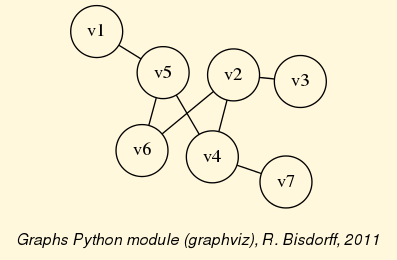
\includegraphics{tutorialGraph.png}\hfill}
\begin{description}
\item[{Chordless cycles may be enumerated in the given graph like follows:}] \leavevmode
\begin{Verbatim}[commandchars=\\\{\}]
\PYG{g+gp}{\PYGZgt{}\PYGZgt{}\PYGZgt{} }\PYG{n}{g} \PYG{o}{=} \PYG{n}{Graph}\PYG{p}{(}\PYG{l+s}{\PYGZsq{}}\PYG{l+s}{tutorialGraph}\PYG{l+s}{\PYGZsq{}}\PYG{p}{)}
\PYG{g+gp}{\PYGZgt{}\PYGZgt{}\PYGZgt{} }\PYG{n}{g}\PYG{o}{.}\PYG{n}{computeChordlessCycles}\PYG{p}{(}\PYG{p}{)}
\PYG{g+go}{Chordless cycle certificate \PYGZhy{}\PYGZhy{}\PYGZgt{}\PYGZgt{}\PYGZgt{}  [\PYGZsq{}v5\PYGZsq{}, \PYGZsq{}v4\PYGZsq{}, \PYGZsq{}v2\PYGZsq{}, \PYGZsq{}v6\PYGZsq{}, \PYGZsq{}v5\PYGZsq{}]}
\PYG{g+go}{[([\PYGZsq{}v5\PYGZsq{}, \PYGZsq{}v4\PYGZsq{}, \PYGZsq{}v2\PYGZsq{}, \PYGZsq{}v6\PYGZsq{}, \PYGZsq{}v5\PYGZsq{}], frozenset(\PYGZob{}\PYGZsq{}v5\PYGZsq{}, \PYGZsq{}v4\PYGZsq{}, \PYGZsq{}v2\PYGZsq{}, \PYGZsq{}v6\PYGZsq{}\PYGZcb{}))]}
\end{Verbatim}

\end{description}


\subsubsection{q-coloring of a graph}
\label{tutorial:q-coloring-of-a-graph}\begin{description}
\item[{And, a 3-coloring of the tutorial graph may be computed and plotted as follows:}] \leavevmode
\begin{Verbatim}[commandchars=\\\{\}]
\PYG{g+gp}{\PYGZgt{}\PYGZgt{}\PYGZgt{} }\PYG{n}{g} \PYG{o}{=} \PYG{n}{Graph}\PYG{p}{(}\PYG{l+s}{\PYGZsq{}}\PYG{l+s}{tutorialGrah}\PYG{l+s}{\PYGZsq{}}\PYG{p}{)}
\PYG{g+gp}{\PYGZgt{}\PYGZgt{}\PYGZgt{} }\PYG{n}{qc} \PYG{o}{=} \PYG{n}{Q\PYGZus{}Coloring}\PYG{p}{(}\PYG{n}{g}\PYG{p}{)}
\PYG{g+go}{Running a Gibbs Sampler for 42 step !}
\PYG{g+go}{The q\PYGZhy{}coloring with 3 colors is feasible !!}
\PYG{g+gp}{\PYGZgt{}\PYGZgt{}\PYGZgt{} }\PYG{n}{qc}\PYG{o}{.}\PYG{n}{showConfiguration}\PYG{p}{(}\PYG{p}{)}
\PYG{g+go}{v5 lightblue}
\PYG{g+go}{v3 gold}
\PYG{g+go}{v7 gold}
\PYG{g+go}{v2 lightblue}
\PYG{g+go}{v4 lightcoral}
\PYG{g+go}{v1 gold}
\PYG{g+go}{v6 lightcoral}
\PYG{g+gp}{\PYGZgt{}\PYGZgt{}\PYGZgt{} }\PYG{n}{qc}\PYG{o}{.}\PYG{n}{exportGraphViz}\PYG{p}{(}\PYG{l+s}{\PYGZsq{}}\PYG{l+s}{tutorial\PYGZhy{}3\PYGZhy{}coloring}\PYG{l+s}{\PYGZsq{}}\PYG{p}{)}
\PYG{g+go}{*\PYGZhy{}\PYGZhy{}\PYGZhy{}\PYGZhy{} exporting a dot file for GraphViz tools \PYGZhy{}\PYGZhy{}\PYGZhy{}\PYGZhy{}\PYGZhy{}\PYGZhy{}\PYGZhy{}\PYGZhy{}\PYGZhy{}*}
\PYG{g+go}{Exporting to tutorial\PYGZhy{}3\PYGZhy{}coloring.dot}
\PYG{g+go}{fdp \PYGZhy{}Tpng tutorial\PYGZhy{}3\PYGZhy{}coloring.dot \PYGZhy{}o tutorial\PYGZhy{}3\PYGZhy{}coloring.png}
\end{Verbatim}

\end{description}

{\hfill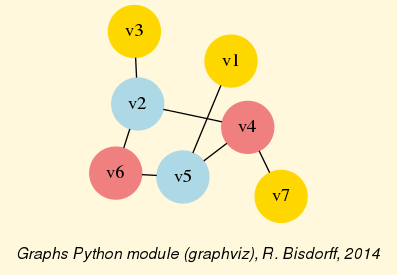
\includegraphics{tutorial-3-coloring.png}\hfill}
\begin{description}
\item[{Actually, with the given tutorial graph instance, a 2-coloring is already feasible:}] \leavevmode
\begin{Verbatim}[commandchars=\\\{\}]
\PYG{g+gp}{\PYGZgt{}\PYGZgt{}\PYGZgt{} }\PYG{n}{qc} \PYG{o}{=} \PYG{n}{Q\PYGZus{}Coloring}\PYG{p}{(}\PYG{n}{g}\PYG{p}{,}\PYG{n}{colors}\PYG{o}{=}\PYG{p}{[}\PYG{l+s}{\PYGZsq{}}\PYG{l+s}{gold}\PYG{l+s}{\PYGZsq{}}\PYG{p}{,}\PYG{l+s}{\PYGZsq{}}\PYG{l+s}{coral}\PYG{l+s}{\PYGZsq{}}\PYG{p}{]}\PYG{p}{)}
\PYG{g+go}{Running a Gibbs Sampler for 42 step !}
\PYG{g+go}{The q\PYGZhy{}coloring with 2 colors is feasible !!}
\PYG{g+gp}{\PYGZgt{}\PYGZgt{}\PYGZgt{} }\PYG{n}{qc}\PYG{o}{.}\PYG{n}{showConfiguration}\PYG{p}{(}\PYG{p}{)}
\PYG{g+go}{v5 gold}
\PYG{g+go}{v3 coral}
\PYG{g+go}{v7 gold}
\PYG{g+go}{v2 gold}
\PYG{g+go}{v4 coral}
\PYG{g+go}{v1 coral}
\PYG{g+go}{v6 coral}
\PYG{g+gp}{\PYGZgt{}\PYGZgt{}\PYGZgt{} }\PYG{n}{qc}\PYG{o}{.}\PYG{n}{exportGraphViz}\PYG{p}{(}\PYG{l+s}{\PYGZsq{}}\PYG{l+s}{tutorial\PYGZhy{}2\PYGZhy{}coloring}\PYG{l+s}{\PYGZsq{}}\PYG{p}{)}
\PYG{g+go}{*\PYGZhy{}\PYGZhy{}\PYGZhy{}\PYGZhy{} exporting a dot file for GraphViz tools \PYGZhy{}\PYGZhy{}\PYGZhy{}\PYGZhy{}\PYGZhy{}\PYGZhy{}\PYGZhy{}\PYGZhy{}\PYGZhy{}*}
\PYG{g+go}{Exporting to tutorial\PYGZhy{}2\PYGZhy{}coloring.dot}
\PYG{g+go}{fdp \PYGZhy{}Tpng tutorial\PYGZhy{}2\PYGZhy{}coloring.dot \PYGZhy{}o tutorial\PYGZhy{}2\PYGZhy{}coloring.png}
\end{Verbatim}

\end{description}

{\hfill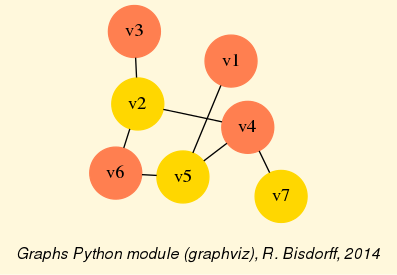
\includegraphics{tutorial-2-coloring.png}\hfill}


\subsubsection{MIS enumeration}
\label{tutorial:mis-enumeration}\begin{description}
\item[{2-colorings define independent sets of vertices that are maximal in cardinality; for short called a \textbf{MIS}. Computing such MISs in a given \code{Graph} instance may be achieved by converting the \code{Graph} instance into a \code{Digraph} instance. Here a \code{self.showMIS()} method is proposed:}] \leavevmode
\begin{Verbatim}[commandchars=\\\{\}]
\PYG{g+gp}{\PYGZgt{}\PYGZgt{}\PYGZgt{} }\PYG{n}{g} \PYG{o}{=} \PYG{n}{Graph}\PYG{p}{(}\PYG{l+s}{\PYGZsq{}}\PYG{l+s}{tutorialGrah}\PYG{l+s}{\PYGZsq{}}\PYG{p}{)}
\PYG{g+gp}{\PYGZgt{}\PYGZgt{}\PYGZgt{} }\PYG{n}{dg} \PYG{o}{=} \PYG{n}{g}\PYG{o}{.}\PYG{n}{graph2Digraph}\PYG{p}{(}\PYG{p}{)}
\PYG{g+gp}{\PYGZgt{}\PYGZgt{}\PYGZgt{} }\PYG{n}{dg}\PYG{o}{.}\PYG{n}{showMIS}\PYG{p}{(}\PYG{p}{)}
\PYG{g+go}{*\PYGZhy{}\PYGZhy{}\PYGZhy{}  Maximal independent choices \PYGZhy{}\PYGZhy{}\PYGZhy{}*}
\PYG{g+go}{[\PYGZsq{}v5\PYGZsq{}, \PYGZsq{}v3\PYGZsq{}, \PYGZsq{}v7\PYGZsq{}]}
\PYG{g+go}{[\PYGZsq{}v5\PYGZsq{}, \PYGZsq{}v7\PYGZsq{}, \PYGZsq{}v2\PYGZsq{}]}
\PYG{g+go}{[\PYGZsq{}v6\PYGZsq{}, \PYGZsq{}v3\PYGZsq{}, \PYGZsq{}v4\PYGZsq{}, \PYGZsq{}v1\PYGZsq{}]}
\PYG{g+go}{[\PYGZsq{}v6\PYGZsq{}, \PYGZsq{}v3\PYGZsq{}, \PYGZsq{}v7\PYGZsq{}, \PYGZsq{}v1\PYGZsq{}]}
\PYG{g+go}{[\PYGZsq{}v7\PYGZsq{}, \PYGZsq{}v2\PYGZsq{}, \PYGZsq{}v1\PYGZsq{}]}
\PYG{g+go}{number of solutions:  5}
\PYG{g+go}{cardinality distribution}
\PYG{g+go}{card.:  [0, 1, 2, 3, 4, 5, 6, 7]}
\PYG{g+go}{freq.:  [0, 0, 0, 3, 2, 0, 0, 0]}
\PYG{g+go}{execution time: 0.00050 sec.}
\PYG{g+go}{Results in self.misset}
\PYG{g+gp}{\PYGZgt{}\PYGZgt{}\PYGZgt{} }\PYG{n}{dg}\PYG{o}{.}\PYG{n}{misset}
\PYG{g+go}{\PYGZob{}frozenset(\PYGZob{}\PYGZsq{}v6\PYGZsq{}, \PYGZsq{}v3\PYGZsq{}, \PYGZsq{}v7\PYGZsq{}, \PYGZsq{}v1\PYGZsq{}\PYGZcb{}),}
\PYG{g+go}{ frozenset(\PYGZob{}\PYGZsq{}v5\PYGZsq{}, \PYGZsq{}v7\PYGZsq{}, \PYGZsq{}v2\PYGZsq{}\PYGZcb{}),}
\PYG{g+go}{ frozenset(\PYGZob{}\PYGZsq{}v6\PYGZsq{}, \PYGZsq{}v3\PYGZsq{}, \PYGZsq{}v4\PYGZsq{}, \PYGZsq{}v1\PYGZsq{}\PYGZcb{}),}
\PYG{g+go}{ frozenset(\PYGZob{}\PYGZsq{}v7\PYGZsq{}, \PYGZsq{}v2\PYGZsq{}, \PYGZsq{}v1\PYGZsq{}\PYGZcb{}),}
\PYG{g+go}{ frozenset(\PYGZob{}\PYGZsq{}v5\PYGZsq{}, \PYGZsq{}v3\PYGZsq{}, \PYGZsq{}v7\PYGZsq{}\PYGZcb{})\PYGZcb{}}
\end{Verbatim}

\end{description}


\subsubsection{Grids and the Ising model}
\label{tutorial:grids-and-the-ising-model}\begin{description}
\item[{Special classes of graphs, like \emph{n} x \emph{m} \textbf{rectangular} or \textbf{triangular grids} are available in the \code{graphs} module. For instance, we may use a Gibbs sampler again for simulating an \textbf{Ising Model} on such a grid:}] \leavevmode
\begin{Verbatim}[commandchars=\\\{\}]
\PYG{g+gp}{\PYGZgt{}\PYGZgt{}\PYGZgt{} }\PYG{k+kn}{from} \PYG{n+nn}{graphs} \PYG{k+kn}{import} \PYG{n}{GridGraph}\PYG{o}{.} \PYG{n}{IsingModel}
\PYG{g+gp}{\PYGZgt{}\PYGZgt{}\PYGZgt{} }\PYG{n}{g} \PYG{o}{=} \PYG{n}{GridGraph}\PYG{p}{(}\PYG{n}{n}\PYG{o}{=}\PYG{l+m+mi}{15}\PYG{p}{,}\PYG{n}{m}\PYG{o}{=}\PYG{l+m+mi}{15}\PYG{p}{)}
\PYG{g+gp}{\PYGZgt{}\PYGZgt{}\PYGZgt{} }\PYG{n}{g}\PYG{o}{.}\PYG{n}{showShort}\PYG{p}{(}\PYG{p}{)}
\PYG{g+go}{*\PYGZhy{}\PYGZhy{}\PYGZhy{}\PYGZhy{}\PYGZhy{} show short \PYGZhy{}\PYGZhy{}\PYGZhy{}\PYGZhy{}\PYGZhy{}\PYGZhy{}\PYGZhy{}\PYGZhy{}\PYGZhy{}\PYGZhy{}\PYGZhy{}\PYGZhy{}\PYGZhy{}\PYGZhy{}*}
\PYG{g+go}{Grid graph    :  grid\PYGZhy{}6\PYGZhy{}6}
\PYG{g+go}{n             :  6}
\PYG{g+go}{m             :  6}
\PYG{g+go}{order         :  36}
\PYG{g+gp}{\PYGZgt{}\PYGZgt{}\PYGZgt{} }\PYG{n}{im} \PYG{o}{=} \PYG{n}{IsingModel}\PYG{p}{(}\PYG{n}{g}\PYG{p}{,}\PYG{n}{beta}\PYG{o}{=}\PYG{l+m+mf}{0.3}\PYG{p}{,}\PYG{n}{nSim}\PYG{o}{=}\PYG{l+m+mi}{100000}\PYG{p}{,}\PYG{n}{Debug}\PYG{o}{=}\PYG{n+nb+bp}{False}\PYG{p}{)}
\PYG{g+go}{Running a Gibbs Sampler for 100000 step !}
\PYG{g+gp}{\PYGZgt{}\PYGZgt{}\PYGZgt{} }\PYG{n}{im}\PYG{o}{.}\PYG{n}{exportGraphViz}\PYG{p}{(}\PYG{n}{colors}\PYG{o}{=}\PYG{p}{[}\PYG{l+s}{\PYGZsq{}}\PYG{l+s}{lightblue}\PYG{l+s}{\PYGZsq{}}\PYG{p}{,}\PYG{l+s}{\PYGZsq{}}\PYG{l+s}{lightcoral}\PYG{l+s}{\PYGZsq{}}\PYG{p}{]}\PYG{p}{)}
\PYG{g+go}{*\PYGZhy{}\PYGZhy{}\PYGZhy{}\PYGZhy{} exporting a dot file for GraphViz tools \PYGZhy{}\PYGZhy{}\PYGZhy{}\PYGZhy{}\PYGZhy{}\PYGZhy{}\PYGZhy{}\PYGZhy{}\PYGZhy{}*}
\PYG{g+go}{Exporting to grid\PYGZhy{}15\PYGZhy{}15\PYGZhy{}ising.dot}
\PYG{g+go}{fdp \PYGZhy{}Tpng grid\PYGZhy{}15\PYGZhy{}15\PYGZhy{}ising.dot \PYGZhy{}o grid\PYGZhy{}15\PYGZhy{}15\PYGZhy{}ising.png}
\end{Verbatim}

\end{description}

{\hfill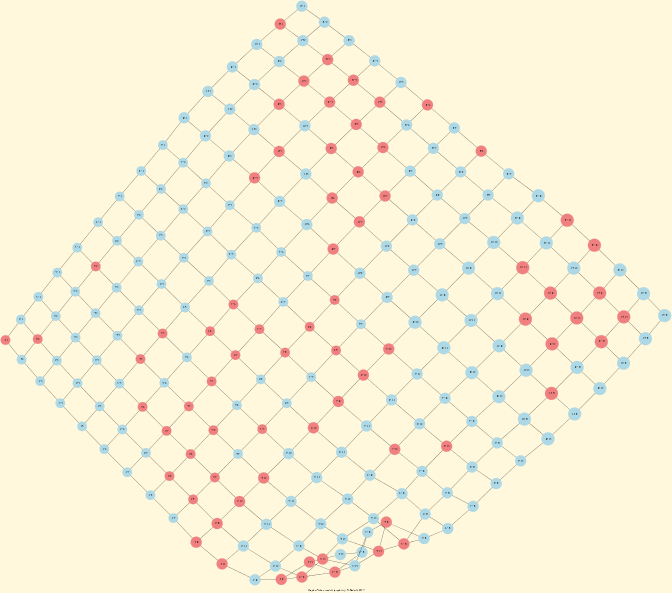
\includegraphics{grid-15-15-ising.png}\hfill}


\subsubsection{Simulating Metropolis random walks}
\label{tutorial:simulating-metropolis-random-walks}\begin{description}
\item[{Finally, we provide a specialisation of the \code{Graph} class for implementing a generic \textbf{Metropolis MCMC} (Monte Carlo Markov Chain) sampler for simulating random walks on a given graph following a given probability  \code{probs = \{‘v1’: x, ‘v2’: y, ...\}} for visiting each vertice.}] \leavevmode
\begin{Verbatim}[commandchars=\\\{\}]
\PYG{g+gp}{\PYGZgt{}\PYGZgt{}\PYGZgt{} }\PYG{k+kn}{from} \PYG{n+nn}{graphs} \PYG{k+kn}{import} \PYG{n}{MetropolisChain}
\PYG{g+gp}{\PYGZgt{}\PYGZgt{}\PYGZgt{} }\PYG{n}{g} \PYG{o}{=} \PYG{n}{Graph}\PYG{p}{(}\PYG{n}{numberOfVertices}\PYG{o}{=}\PYG{l+m+mi}{5}\PYG{p}{,}\PYG{n}{edgeProbability}\PYG{o}{=}\PYG{l+m+mf}{0.5}\PYG{p}{)}
\PYG{g+gp}{\PYGZgt{}\PYGZgt{}\PYGZgt{} }\PYG{n}{g}\PYG{o}{.}\PYG{n}{showShort}\PYG{p}{(}\PYG{p}{)}
\PYG{g+go}{*\PYGZhy{}\PYGZhy{}\PYGZhy{}\PYGZhy{} short description of the graph \PYGZhy{}\PYGZhy{}\PYGZhy{}\PYGZhy{}*}
\PYG{g+go}{Name             : \PYGZsq{}randomGraph\PYGZsq{}}
\PYG{g+go}{Vertices         :  [\PYGZsq{}v1\PYGZsq{}, \PYGZsq{}v2\PYGZsq{}, \PYGZsq{}v3\PYGZsq{}, \PYGZsq{}v4\PYGZsq{}, \PYGZsq{}v5\PYGZsq{}]}
\PYG{g+go}{Valuation domain :  \PYGZob{}\PYGZsq{}max\PYGZsq{}: 1, \PYGZsq{}med\PYGZsq{}: 0, \PYGZsq{}min\PYGZsq{}: \PYGZhy{}1\PYGZcb{}}
\PYG{g+go}{Gamma function   :}
\PYG{g+go}{v1 \PYGZhy{}\PYGZgt{} [\PYGZsq{}v2\PYGZsq{}, \PYGZsq{}v3\PYGZsq{}, \PYGZsq{}v4\PYGZsq{}]}
\PYG{g+go}{v2 \PYGZhy{}\PYGZgt{} [\PYGZsq{}v1\PYGZsq{}, \PYGZsq{}v4\PYGZsq{}]}
\PYG{g+go}{v3 \PYGZhy{}\PYGZgt{} [\PYGZsq{}v5\PYGZsq{}, \PYGZsq{}v1\PYGZsq{}]}
\PYG{g+go}{v4 \PYGZhy{}\PYGZgt{} [\PYGZsq{}v2\PYGZsq{}, \PYGZsq{}v5\PYGZsq{}, \PYGZsq{}v1\PYGZsq{}]}
\PYG{g+go}{v5 \PYGZhy{}\PYGZgt{} [\PYGZsq{}v3\PYGZsq{}, \PYGZsq{}v4\PYGZsq{}]}
\PYG{g+gp}{\PYGZgt{}\PYGZgt{}\PYGZgt{} }\PYG{n}{probs} \PYG{o}{=} \PYG{p}{\PYGZob{}}\PYG{p}{\PYGZcb{}}  \PYG{c}{\PYGZsh{} initialise a potential stationary probability vector}
\PYG{g+gp}{\PYGZgt{}\PYGZgt{}\PYGZgt{} }\PYG{n}{n} \PYG{o}{=} \PYG{n}{g}\PYG{o}{.}\PYG{n}{order} \PYG{c}{\PYGZsh{} for instance: probs[v\PYGZus{}i] = n\PYGZhy{}i/Sum(1:n) for i in 1:n}
\PYG{g+gp}{\PYGZgt{}\PYGZgt{}\PYGZgt{} }\PYG{n}{i} \PYG{o}{=} \PYG{l+m+mi}{0}
\PYG{g+gp}{\PYGZgt{}\PYGZgt{}\PYGZgt{} }\PYG{n}{verticesList} \PYG{o}{=} \PYG{p}{[}\PYG{n}{x} \PYG{k}{for} \PYG{n}{x} \PYG{o+ow}{in} \PYG{n}{g}\PYG{o}{.}\PYG{n}{vertices}\PYG{p}{]}
\PYG{g+gp}{\PYGZgt{}\PYGZgt{}\PYGZgt{} }\PYG{n}{verticesList}\PYG{o}{.}\PYG{n}{sort}\PYG{p}{(}\PYG{p}{)}
\PYG{g+gp}{\PYGZgt{}\PYGZgt{}\PYGZgt{} }\PYG{k}{for} \PYG{n}{v} \PYG{o+ow}{in} \PYG{n}{verticesList}\PYG{p}{:}
\PYG{g+gp}{... }    \PYG{n}{probs}\PYG{p}{[}\PYG{n}{v}\PYG{p}{]} \PYG{o}{=} \PYG{p}{(}\PYG{n}{n} \PYG{o}{\PYGZhy{}} \PYG{n}{i}\PYG{p}{)}\PYG{o}{/}\PYG{p}{(}\PYG{n}{n}\PYG{o}{*}\PYG{p}{(}\PYG{n}{n}\PYG{o}{+}\PYG{l+m+mi}{1}\PYG{p}{)}\PYG{o}{/}\PYG{l+m+mi}{2}\PYG{p}{)}
\PYG{g+gp}{... }    \PYG{n}{i} \PYG{o}{+}\PYG{o}{=} \PYG{l+m+mi}{1}
\PYG{g+gp}{\PYGZgt{}\PYGZgt{}\PYGZgt{} }\PYG{n}{met} \PYG{o}{=} \PYG{n}{MetropolisChain}\PYG{p}{(}\PYG{n}{g}\PYG{p}{,}\PYG{n}{probs}\PYG{p}{)}
\PYG{g+gp}{\PYGZgt{}\PYGZgt{}\PYGZgt{} }\PYG{n}{frequency} \PYG{o}{=} \PYG{n}{met}\PYG{o}{.}\PYG{n}{checkSampling}\PYG{p}{(}\PYG{n}{verticesList}\PYG{p}{[}\PYG{l+m+mi}{0}\PYG{p}{]}\PYG{p}{,}\PYG{n}{nSim}\PYG{o}{=}\PYG{l+m+mi}{30000}\PYG{p}{)}
\PYG{g+gp}{\PYGZgt{}\PYGZgt{}\PYGZgt{} }\PYG{k}{for} \PYG{n}{v} \PYG{o+ow}{in} \PYG{n}{verticesList}\PYG{p}{:}
\PYG{g+gp}{... }    \PYG{k}{print}\PYG{p}{(}\PYG{n}{v}\PYG{p}{,}\PYG{n}{probs}\PYG{p}{[}\PYG{n}{v}\PYG{p}{]}\PYG{p}{,}\PYG{n}{frequency}\PYG{p}{[}\PYG{n}{v}\PYG{p}{]}\PYG{p}{)}
\PYG{g+go}{v1 0.3333 0.3343}
\PYG{g+go}{v2 0.2666 0.2680}
\PYG{g+go}{v3 0.2    0.2030}
\PYG{g+go}{v4 0.1333 0.1311}
\PYG{g+go}{v5 0.0666 0.0635}
\PYG{g+gp}{\PYGZgt{}\PYGZgt{}\PYGZgt{} }\PYG{n}{met}\PYG{o}{.}\PYG{n}{showTransitionMatrix}\PYG{p}{(}\PYG{p}{)}
\PYG{g+go}{* \PYGZhy{}\PYGZhy{}\PYGZhy{}\PYGZhy{} Transition Matrix \PYGZhy{}\PYGZhy{}\PYGZhy{}\PYGZhy{}\PYGZhy{}}
\PYG{g+go}{  Pij  \textbar{} \PYGZsq{}v1\PYGZsq{}    \PYGZsq{}v2\PYGZsq{}    \PYGZsq{}v3\PYGZsq{}    \PYGZsq{}v4\PYGZsq{}    \PYGZsq{}v5\PYGZsq{}}
\PYG{g+go}{  \PYGZhy{}\PYGZhy{}\PYGZhy{}\PYGZhy{}\PYGZhy{}\textbar{}\PYGZhy{}\PYGZhy{}\PYGZhy{}\PYGZhy{}\PYGZhy{}\PYGZhy{}\PYGZhy{}\PYGZhy{}\PYGZhy{}\PYGZhy{}\PYGZhy{}\PYGZhy{}\PYGZhy{}\PYGZhy{}\PYGZhy{}\PYGZhy{}\PYGZhy{}\PYGZhy{}\PYGZhy{}\PYGZhy{}\PYGZhy{}\PYGZhy{}\PYGZhy{}\PYGZhy{}\PYGZhy{}\PYGZhy{}\PYGZhy{}\PYGZhy{}\PYGZhy{}\PYGZhy{}\PYGZhy{}\PYGZhy{}\PYGZhy{}\PYGZhy{}\PYGZhy{}\PYGZhy{}\PYGZhy{}}
\PYG{g+go}{  \PYGZsq{}v1\PYGZsq{} \textbar{}  0.23   0.33    0.30    0.13    0.00}
\PYG{g+go}{  \PYGZsq{}v2\PYGZsq{} \textbar{}  0.42   0.42    0.00    0.17    0.00}
\PYG{g+go}{  \PYGZsq{}v3\PYGZsq{} \textbar{}  0.50   0.00    0.33    0.00    0.17}
\PYG{g+go}{  \PYGZsq{}v4\PYGZsq{} \textbar{}  0.33   0.33    0.00    0.08    0.25}
\PYG{g+go}{  \PYGZsq{}v5\PYGZsq{} \textbar{}  0.00   0.00    0.50    0.50    0.00}
\end{Verbatim}

\end{description}

The \code{checkSampling()} method generates a randomwalk of \emph{nSim=30000} steps on the given graph and records by the way the observed relative frequency with which each vertice is passed by. In this exmaple, the stationary transition probability distribution, shown by the \code{showTransitionMatrix()} method above, is quite adequately simulated.

For more technical information and more code examples, look into the technical documentation of the {\hyperref[techDoc:graphs-label]{\emph{graphs module}}}. For the readers interested in algorithmic applications of Markov Chains we may may recommend consulting O. Häggström's 2002 book: {\hyperref[tutorial:fmcaa]{{[}FMCAA{]}}}.

Back to {\hyperref[tutorial:tutorial-label]{\emph{Content}}}


\subsection{Computing the winner of an election}
\label{tutorial:computing-the-winner-of-an-election}\label{tutorial:linearvoting-label}

\subsubsection{Linear voting profiles}
\label{tutorial:linear-voting-profiles}
The {\hyperref[techDoc:votingdigraphs-label]{\emph{votingDigraphs module}}} provides resources for handling election results {\hyperref[tutorial:adt-l2]{{[}ADT-L2{]}}}, like the \code{LinearVotingProfile} class. We consider an election involving a finite set of candidates and finite set of weighted voters, who express their voting preferences in a complete linear ranking (without ties) of the candidates. The data is internally stored in two Python dictionaries, one for the candidates and another one for the linear ballots:

\begin{Verbatim}[commandchars=\\\{\}]
candidates = \PYGZob{}\PYGZsq{}a\PYGZsq{}: ,\PYGZsq{}b\PYGZsq{}:  ,\PYGZsq{}c\PYGZsq{}, ..., ...\PYGZcb{}
voters = \PYGZob{}\PYGZsq{}1\PYGZsq{}:\PYGZob{}\PYGZsq{}weight\PYGZsq{}:1.0\PYGZcb{},\PYGZsq{}2\PYGZsq{}:\PYGZob{}\PYGZsq{}weight\PYGZsq{}:1.0\PYGZcb{}, ...\PYGZcb{}
\PYGZsh{}\PYGZsh{} each voter specifies a linearly ranked list of candidates
\PYGZsh{}\PYGZsh{} from the best to the worst (without ties
linearBallot = \PYGZob{}
\PYGZsq{}1\PYGZsq{} : [\PYGZsq{}b\PYGZsq{},\PYGZsq{}c\PYGZsq{},\PYGZsq{}a\PYGZsq{}, ...],
\PYGZsq{}2\PYGZsq{} : [\PYGZsq{}a\PYGZsq{},\PYGZsq{}b\PYGZsq{},\PYGZsq{}c\PYGZsq{}, ...],
...
\PYGZcb{}
\end{Verbatim}
\begin{description}
\item[{The module provides a class for generating random instances of the \code{LinearVotingProfile} class. In an interactive Python session we may obtain for the election of 3 candidates by 5 voters the following result:}] \leavevmode
\begin{Verbatim}[commandchars=\\\{\}]
\PYG{g+gp}{\PYGZgt{}\PYGZgt{}\PYGZgt{} }\PYG{k+kn}{from} \PYG{n+nn}{votingDigraphs} \PYG{k+kn}{import} \PYG{o}{*}
\PYG{g+gp}{\PYGZgt{}\PYGZgt{}\PYGZgt{} }\PYG{n}{v} \PYG{o}{=} \PYG{n}{RandomLinearVotingProfile}\PYG{p}{(}\PYG{n}{numberOfVoters}\PYG{o}{=}\PYG{l+m+mi}{5}\PYG{p}{,}\PYG{n}{numberOfCandidates}\PYG{o}{=}\PYG{l+m+mi}{3}\PYG{p}{)}
\PYG{g+gp}{\PYGZgt{}\PYGZgt{}\PYGZgt{} }\PYG{n}{v}\PYG{o}{.}\PYG{n}{candidates}
\PYG{g+go}{\PYGZob{}\PYGZsq{}a2\PYGZsq{}: \PYGZob{}\PYGZsq{}name\PYGZsq{}: \PYGZsq{}a2\PYGZsq{}\PYGZcb{}, \PYGZsq{}a3\PYGZsq{}: \PYGZob{}\PYGZsq{}name\PYGZsq{}: \PYGZsq{}a3\PYGZsq{}\PYGZcb{}, \PYGZsq{}a1\PYGZsq{}: \PYGZob{}\PYGZsq{}name\PYGZsq{}: \PYGZsq{}a1\PYGZsq{}\PYGZcb{}\PYGZcb{}}
\PYG{g+gp}{\PYGZgt{}\PYGZgt{}\PYGZgt{} }\PYG{n}{v}\PYG{o}{.}\PYG{n}{voters}
\PYG{g+go}{\PYGZob{}\PYGZsq{}v4\PYGZsq{}: \PYGZob{}\PYGZsq{}weight\PYGZsq{}: 1.0\PYGZcb{}, \PYGZsq{}v3\PYGZsq{}: \PYGZob{}\PYGZsq{}weight\PYGZsq{}: 1.0\PYGZcb{},}
\PYG{g+go}{ \PYGZsq{}v1\PYGZsq{}: \PYGZob{}\PYGZsq{}weight\PYGZsq{}: 1.0\PYGZcb{}, \PYGZsq{}v5\PYGZsq{}: \PYGZob{}\PYGZsq{}weight\PYGZsq{}: 1.0\PYGZcb{},}
\PYG{g+go}{ \PYGZsq{}v2\PYGZsq{}: \PYGZob{}\PYGZsq{}weight\PYGZsq{}: 1.0\PYGZcb{}\PYGZcb{}}
\PYG{g+gp}{\PYGZgt{}\PYGZgt{}\PYGZgt{} }\PYG{n}{v}\PYG{o}{.}\PYG{n}{linearBallot}
\PYG{g+go}{\PYGZob{}\PYGZsq{}v4\PYGZsq{}: [\PYGZsq{}a1\PYGZsq{}, \PYGZsq{}a3\PYGZsq{}, \PYGZsq{}a2\PYGZsq{}], \PYGZsq{}v3\PYGZsq{}: [\PYGZsq{}a1\PYGZsq{}, \PYGZsq{}a3\PYGZsq{}, \PYGZsq{}a2\PYGZsq{}], \PYGZsq{}v1\PYGZsq{}: [\PYGZsq{}a1\PYGZsq{}, \PYGZsq{}a2\PYGZsq{}, \PYGZsq{}a3\PYGZsq{}],}
\PYG{g+go}{ \PYGZsq{}v5\PYGZsq{}: [\PYGZsq{}a2\PYGZsq{}, \PYGZsq{}a3\PYGZsq{}, \PYGZsq{}a1\PYGZsq{}], \PYGZsq{}v2\PYGZsq{}: [\PYGZsq{}a3\PYGZsq{}, \PYGZsq{}a2\PYGZsq{}, \PYGZsq{}a1\PYGZsq{}]\PYGZcb{}}
\PYG{g+go}{ \PYGZgt{}\PYGZgt{}\PYGZgt{} ...}
\end{Verbatim}

\item[{Notice that in this example, all voters are considered to be equi-significant. Their linear ballots can be viewd with the \code{showLinearBallots} method:}] \leavevmode
\begin{Verbatim}[commandchars=\\\{\}]
\PYG{g+gp}{\PYGZgt{}\PYGZgt{}\PYGZgt{} }\PYG{n}{v}\PYG{o}{.}\PYG{n}{showLinearBallots}\PYG{p}{(}\PYG{p}{)}
\PYG{g+go}{voters(weight)       candidates rankings}
\PYG{g+go}{v4(1.0):     [\PYGZsq{}a1\PYGZsq{}, \PYGZsq{}a2\PYGZsq{}, \PYGZsq{}a3\PYGZsq{}]}
\PYG{g+go}{v3(1.0):     [\PYGZsq{}a1\PYGZsq{}, \PYGZsq{}a3\PYGZsq{}, \PYGZsq{}a2\PYGZsq{}]}
\PYG{g+go}{v1(1.0):     [\PYGZsq{}a2\PYGZsq{}, \PYGZsq{}a1\PYGZsq{}, \PYGZsq{}a3\PYGZsq{}]}
\PYG{g+go}{v5(1.0):     [\PYGZsq{}a3\PYGZsq{}, \PYGZsq{}a1\PYGZsq{}, \PYGZsq{}a2\PYGZsq{}]}
\PYG{g+go}{v2(1.0):     [\PYGZsq{}a3\PYGZsq{}, \PYGZsq{}a1\PYGZsq{}, \PYGZsq{}a2\PYGZsq{}]}
\PYG{g+gp}{\PYGZgt{}\PYGZgt{}\PYGZgt{} }\PYG{o}{.}\PYG{o}{.}\PYG{o}{.}
\end{Verbatim}

\item[{Editing of the linear voting profile may be acheived by storing the data in a file, edit it, and reload it again:}] \leavevmode
\begin{Verbatim}[commandchars=\\\{\}]
\PYG{g+gp}{\PYGZgt{}\PYGZgt{}\PYGZgt{} }\PYG{n}{v}\PYG{o}{.}\PYG{n}{save}\PYG{p}{(}\PYG{l+s}{\PYGZsq{}}\PYG{l+s}{tutorialLinearVotingProfile}\PYG{l+s}{\PYGZsq{}}\PYG{p}{)}
\PYG{g+go}{*\PYGZhy{}\PYGZhy{}\PYGZhy{} Saving linear profile in file: \PYGZlt{}tutorialLinearVotingProfile.py\PYGZgt{} \PYGZhy{}\PYGZhy{}\PYGZhy{}*}
\PYG{g+gp}{\PYGZgt{}\PYGZgt{}\PYGZgt{} }\PYG{n}{v} \PYG{o}{=} \PYG{n}{LinearVotingProfile}\PYG{p}{(}\PYG{l+s}{\PYGZsq{}}\PYG{l+s}{tutorialLinearVotingProfile}\PYG{l+s}{\PYGZsq{}}\PYG{p}{)}
\end{Verbatim}

\end{description}


\subsubsection{Computing the winner}
\label{tutorial:computing-the-winner}\begin{description}
\item[{We may easily compute \textbf{uninominal votes}, i.e. how many times a candidate was ranked first, and see who is consequently the \textbf{simple majority} winner(s) in this election.}] \leavevmode
\begin{Verbatim}[commandchars=\\\{\}]
\PYG{g+gp}{\PYGZgt{}\PYGZgt{}\PYGZgt{} }\PYG{n}{v}\PYG{o}{.}\PYG{n}{computeUninominalVotes}\PYG{p}{(}\PYG{p}{)}
\PYG{g+go}{\PYGZob{}\PYGZsq{}a2\PYGZsq{}: 1.0, \PYGZsq{}a1\PYGZsq{}: 2.0, \PYGZsq{}a3\PYGZsq{}: 2.0\PYGZcb{}}
\PYG{g+gp}{\PYGZgt{}\PYGZgt{}\PYGZgt{} }\PYG{n}{v}\PYG{o}{.}\PYG{n}{computeSimpleMajorityWinner}\PYG{p}{(}\PYG{p}{)}
\PYG{g+go}{[\PYGZsq{}a1\PYGZsq{},\PYGZsq{}a3\PYGZsq{}]}
\PYG{g+gp}{\PYGZgt{}\PYGZgt{}\PYGZgt{} }\PYG{o}{.}\PYG{o}{.}\PYG{o}{.}
\end{Verbatim}

\item[{As we observe no absolute majority (3/5) of votes for any of the three candidate, we may look for the \textbf{instant runoff} winner instead (see {\hyperref[tutorial:adt-l2]{{[}ADT-L2{]}}}):}] \leavevmode
\begin{Verbatim}[commandchars=\\\{\}]
\PYG{g+gp}{\PYGZgt{}\PYGZgt{}\PYGZgt{} }\PYG{n}{v}\PYG{o}{.}\PYG{n}{computeInstantRunoffWinner}\PYG{p}{(}\PYG{p}{)}
\PYG{g+go}{[\PYGZsq{}a1\PYGZsq{}]}
\PYG{g+gp}{\PYGZgt{}\PYGZgt{}\PYGZgt{} }\PYG{o}{.}\PYG{o}{.}\PYG{o}{.}
\end{Verbatim}

\item[{We may also follow the Chevalier de Borda's advice and, after a \textbf{rank analysis} of the linear ballots, compute the \textbf{Borda score} of each candidate and hence determine the \textbf{Borda winner(s)}:}] \leavevmode
\begin{Verbatim}[commandchars=\\\{\}]
\PYG{g+gp}{\PYGZgt{}\PYGZgt{}\PYGZgt{} }\PYG{n}{v}\PYG{o}{.}\PYG{n}{computeRankAnalysis}\PYG{p}{(}\PYG{p}{)}
\PYG{g+go}{\PYGZob{}\PYGZsq{}a2\PYGZsq{}: [1.0, 1.0, 3.0], \PYGZsq{}a1\PYGZsq{}: [2.0, 3.0, 0], \PYGZsq{}a3\PYGZsq{}: [2.0, 1.0, 2.0]\PYGZcb{}}
\PYG{g+gp}{\PYGZgt{}\PYGZgt{}\PYGZgt{} }\PYG{n}{v}\PYG{o}{.}\PYG{n}{computeBordaScores}\PYG{p}{(}\PYG{p}{)}
\PYG{g+go}{\PYGZob{}\PYGZsq{}a2\PYGZsq{}: 12.0, \PYGZsq{}a1\PYGZsq{}: 8.0, \PYGZsq{}a3\PYGZsq{}: 10.0\PYGZcb{}}
\PYG{g+gp}{\PYGZgt{}\PYGZgt{}\PYGZgt{} }\PYG{n}{v}\PYG{o}{.}\PYG{n}{computeBordaWinners}\PYG{p}{(}\PYG{p}{)}
\PYG{g+go}{[\PYGZsq{}a1\PYGZsq{}]}
\PYG{g+gp}{\PYGZgt{}\PYGZgt{}\PYGZgt{} }\PYG{o}{.}\PYG{o}{.}\PYG{o}{.}
\end{Verbatim}

\end{description}


\subsubsection{The Condorcet winner}
\label{tutorial:the-condorcet-winner}\begin{description}
\item[{In our randomly generated election results, we are lucky: The instant runoff winner and the Borda winner both are candidate \emph{a1}. However, we could also follow the Marquis de Condorcet's advice, and compute the \textbf{majority margins} obtained by voting for each individual pair of candidates. For instance, candidate \emph{a1} is ranked four times before and once behind candidate \emph{a2}. Hence the majority margin \emph{M(a1,a2)} is 4 - 1 = +3. These majority margins define on the set of candidates what we call the \textbf{Condorcet digraph}, a specialization of the \code{Digraph} class for handling such pairwise majority margins:}] \leavevmode
\begin{Verbatim}[commandchars=\\\{\}]
\PYG{g+gp}{\PYGZgt{}\PYGZgt{}\PYGZgt{} }\PYG{n}{cdg} \PYG{o}{=} \PYG{n}{CondorcetDigraph}\PYG{p}{(}\PYG{n}{v}\PYG{p}{,}\PYG{n}{hasIntegerValuation}\PYG{o}{=}\PYG{n+nb+bp}{True}\PYG{p}{)}
\PYG{g+gp}{\PYGZgt{}\PYGZgt{}\PYGZgt{} }\PYG{n}{cdg}\PYG{o}{.}\PYG{n}{showAll}\PYG{p}{(}\PYG{p}{)}
\PYG{g+go}{*\PYGZhy{}\PYGZhy{}\PYGZhy{}\PYGZhy{}\PYGZhy{} show detail \PYGZhy{}\PYGZhy{}\PYGZhy{}\PYGZhy{}\PYGZhy{}\PYGZhy{}\PYGZhy{}\PYGZhy{}\PYGZhy{}\PYGZhy{}\PYGZhy{}\PYGZhy{}\PYGZhy{}*}
\PYG{g+go}{Digraph          : rel\PYGZus{}randLinearProfile}
\PYG{g+go}{*\PYGZhy{}\PYGZhy{}\PYGZhy{}\PYGZhy{} Actions \PYGZhy{}\PYGZhy{}\PYGZhy{}\PYGZhy{}*}
\PYG{g+go}{[\PYGZsq{}a1\PYGZsq{}, \PYGZsq{}a2\PYGZsq{}, \PYGZsq{}a3\PYGZsq{}]}
\PYG{g+go}{*\PYGZhy{}\PYGZhy{}\PYGZhy{}\PYGZhy{} Characteristic valuation domain \PYGZhy{}\PYGZhy{}\PYGZhy{}\PYGZhy{}*}
\PYG{g+go}{\PYGZob{}\PYGZsq{}hasIntegerValuation\PYGZsq{}: True,}
\PYG{g+go}{\PYGZsq{}max\PYGZsq{}: Decimal(\PYGZsq{}5.0\PYGZsq{}),}
\PYG{g+go}{\PYGZsq{}min\PYGZsq{}: Decimal(\PYGZsq{}\PYGZhy{}5.0\PYGZsq{}),}
\PYG{g+go}{\PYGZsq{}med\PYGZsq{}: Decimal(\PYGZsq{}0\PYGZsq{})\PYGZcb{}}
\PYG{g+go}{* \PYGZhy{}\PYGZhy{}\PYGZhy{}\PYGZhy{} Relation Table \PYGZhy{}\PYGZhy{}\PYGZhy{}\PYGZhy{}}
\PYG{g+go}{ M(x,y) \textbar{}  \PYGZsq{}a1\PYGZsq{} \PYGZsq{}a2\PYGZsq{} \PYGZsq{}a3\PYGZsq{}}
\PYG{g+go}{ \PYGZhy{}\PYGZhy{}\PYGZhy{}\PYGZhy{}\PYGZhy{}\PYGZhy{}\PYGZhy{}\textbar{}\PYGZhy{}\PYGZhy{}\PYGZhy{}\PYGZhy{}\PYGZhy{}\PYGZhy{}\PYGZhy{}\PYGZhy{}\PYGZhy{}\PYGZhy{}\PYGZhy{}\PYGZhy{}\PYGZhy{}\PYGZhy{}\PYGZhy{}\PYGZhy{}\PYGZhy{}}
\PYG{g+go}{   \PYGZsq{}a1\PYGZsq{} \textbar{}   \PYGZhy{}    3    1}
\PYG{g+go}{   \PYGZsq{}a2\PYGZsq{} \textbar{}  \PYGZhy{}3    \PYGZhy{}   \PYGZhy{}1}
\PYG{g+go}{   \PYGZsq{}a3\PYGZsq{} \textbar{}  \PYGZhy{}1    1    \PYGZhy{}}
\end{Verbatim}

\item[{A candidate \emph{x}, showing a positive majority margin \emph{M(x,y)}, is beating candidate \emph{y}  with an absolute majority in a pairwise voting. Hence, a candidate showing only positive terms in her row in the Condorcet digraph relation table, beats all other candidates with absolute majority of votes. Condorcet recommends to declare this candidate (is always unique, why?) the winner of the election. Here we are lucky, it is again candidate \emph{a1} who is hence the \textbf{Condorcet winner}:}] \leavevmode
\begin{Verbatim}[commandchars=\\\{\}]
\PYG{g+gp}{\PYGZgt{}\PYGZgt{}\PYGZgt{} }\PYG{n}{cdg}\PYG{o}{.}\PYG{n}{computeCondorcetWinner}\PYG{p}{(}\PYG{p}{)}
\PYG{g+go}{[\PYGZsq{}a1\PYGZsq{}]}
\end{Verbatim}

\item[{By seeing the majority margins like a bipolarly-valued characteristic function for a global preference relation defined on the set of canditates, we may use all operational resources of the generic \code{Digraph} class (see {\hyperref[tutorial:digraphs-tutorial-label]{\emph{Working with the digraphs module}}}), and especially its \code{exportGraphViz} method \footnotemark[1], for visualizing an election result:}] \leavevmode
\begin{Verbatim}[commandchars=\\\{\}]
\PYG{g+gp}{\PYGZgt{}\PYGZgt{}\PYGZgt{} }\PYG{n}{cdg}\PYG{o}{.}\PYG{n}{exportGraphViz}\PYG{p}{(}\PYG{l+s}{\PYGZsq{}}\PYG{l+s}{tutorialLinearBallots}\PYG{l+s}{\PYGZsq{}}\PYG{p}{)}
\PYG{g+go}{*\PYGZhy{}\PYGZhy{}\PYGZhy{}\PYGZhy{} exporting a dot file for GraphViz tools \PYGZhy{}\PYGZhy{}\PYGZhy{}\PYGZhy{}\PYGZhy{}\PYGZhy{}\PYGZhy{}\PYGZhy{}\PYGZhy{}*}
\PYG{g+go}{Exporting to tutorialLinearBallots.dot}
\PYG{g+go}{dot \PYGZhy{}Grankdir=BT \PYGZhy{}Tpng tutorialLinearBallots.dot \PYGZhy{}o tutorialLinearBallots.png}
\end{Verbatim}

\end{description}

{\hfill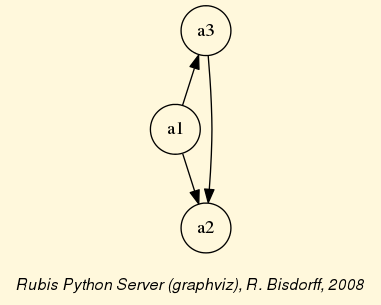
\includegraphics{tutorialLinearBallots.png}\hfill}


\subsubsection{Cyclic social preferences}
\label{tutorial:cyclic-social-preferences}\begin{description}
\item[{Usually, when aggregating linear ballots, there appear cyclic social preferences. Let us consider for instance the following linear voting profile and construct the corresponding Condorcet digraph:}] \leavevmode
\begin{Verbatim}[commandchars=\\\{\}]
\PYG{g+gp}{\PYGZgt{}\PYGZgt{}\PYGZgt{} }\PYG{n}{v}\PYG{o}{.}\PYG{n}{showLinearBallots}\PYG{p}{(}\PYG{p}{)}
\PYG{g+go}{voters(weight)       candidates rankings}
\PYG{g+go}{v1(1.0):     [\PYGZsq{}a1\PYGZsq{}, \PYGZsq{}a3\PYGZsq{}, \PYGZsq{}a5\PYGZsq{}, \PYGZsq{}a2\PYGZsq{}, \PYGZsq{}a4\PYGZsq{}]}
\PYG{g+go}{v2(1.0):     [\PYGZsq{}a1\PYGZsq{}, \PYGZsq{}a2\PYGZsq{}, \PYGZsq{}a4\PYGZsq{}, \PYGZsq{}a3\PYGZsq{}, \PYGZsq{}a5\PYGZsq{}]}
\PYG{g+go}{v3(1.0):     [\PYGZsq{}a5\PYGZsq{}, \PYGZsq{}a2\PYGZsq{}, \PYGZsq{}a4\PYGZsq{}, \PYGZsq{}a3\PYGZsq{}, \PYGZsq{}a1\PYGZsq{}]}
\PYG{g+go}{v4(1.0):     [\PYGZsq{}a3\PYGZsq{}, \PYGZsq{}a4\PYGZsq{}, \PYGZsq{}a1\PYGZsq{}, \PYGZsq{}a5\PYGZsq{}, \PYGZsq{}a2\PYGZsq{}]}
\PYG{g+go}{v5(1.0):     [\PYGZsq{}a4\PYGZsq{}, \PYGZsq{}a2\PYGZsq{}, \PYGZsq{}a3\PYGZsq{}, \PYGZsq{}a5\PYGZsq{}, \PYGZsq{}a1\PYGZsq{}]}
\PYG{g+go}{v6(1.0):     [\PYGZsq{}a2\PYGZsq{}, \PYGZsq{}a4\PYGZsq{}, \PYGZsq{}a5\PYGZsq{}, \PYGZsq{}a1\PYGZsq{}, \PYGZsq{}a3\PYGZsq{}]}
\PYG{g+go}{v7(1.0):     [\PYGZsq{}a5\PYGZsq{}, \PYGZsq{}a4\PYGZsq{}, \PYGZsq{}a3\PYGZsq{}, \PYGZsq{}a1\PYGZsq{}, \PYGZsq{}a2\PYGZsq{}]}
\PYG{g+go}{v8(1.0):     [\PYGZsq{}a2\PYGZsq{}, \PYGZsq{}a4\PYGZsq{}, \PYGZsq{}a5\PYGZsq{}, \PYGZsq{}a1\PYGZsq{}, \PYGZsq{}a3\PYGZsq{}]}
\PYG{g+go}{v9(1.0):     [\PYGZsq{}a5\PYGZsq{}, \PYGZsq{}a3\PYGZsq{}, \PYGZsq{}a4\PYGZsq{}, \PYGZsq{}a1\PYGZsq{}, \PYGZsq{}a2\PYGZsq{}]}
\PYG{g+gp}{\PYGZgt{}\PYGZgt{}\PYGZgt{} }\PYG{n}{cdg} \PYG{o}{=} \PYG{n}{CondorcetDigraph}\PYG{p}{(}\PYG{n}{v}\PYG{p}{)}
\PYG{g+gp}{\PYGZgt{}\PYGZgt{}\PYGZgt{} }\PYG{n}{cdg}\PYG{o}{.}\PYG{n}{showRelationTable}\PYG{p}{(}\PYG{p}{)}
\PYG{g+go}{* \PYGZhy{}\PYGZhy{}\PYGZhy{}\PYGZhy{} Relation Table \PYGZhy{}\PYGZhy{}\PYGZhy{}\PYGZhy{}\PYGZhy{}}
\PYG{g+go}{  S   \textbar{}  \PYGZsq{}a1\PYGZsq{}   \PYGZsq{}a2\PYGZsq{}   \PYGZsq{}a3\PYGZsq{}   \PYGZsq{}a4\PYGZsq{}    \PYGZsq{}a5\PYGZsq{}}
\PYG{g+go}{\PYGZhy{}\PYGZhy{}\PYGZhy{}\PYGZhy{}\PYGZhy{}\PYGZhy{}\textbar{}\PYGZhy{}\PYGZhy{}\PYGZhy{}\PYGZhy{}\PYGZhy{}\PYGZhy{}\PYGZhy{}\PYGZhy{}\PYGZhy{}\PYGZhy{}\PYGZhy{}\PYGZhy{}\PYGZhy{}\PYGZhy{}\PYGZhy{}\PYGZhy{}\PYGZhy{}\PYGZhy{}\PYGZhy{}\PYGZhy{}\PYGZhy{}\PYGZhy{}\PYGZhy{}\PYGZhy{}\PYGZhy{}\PYGZhy{}\PYGZhy{}\PYGZhy{}\PYGZhy{}\PYGZhy{}\PYGZhy{}\PYGZhy{}\PYGZhy{}\PYGZhy{}\PYGZhy{}\PYGZhy{}\PYGZhy{}\PYGZhy{}\PYGZhy{}\PYGZhy{}}
\PYG{g+go}{\PYGZsq{}a1\PYGZsq{}  \textbar{}   \PYGZhy{}     0.11  \PYGZhy{}0.11  \PYGZhy{}0.56   \PYGZhy{}0.33}
\PYG{g+go}{\PYGZsq{}a2\PYGZsq{}  \textbar{} \PYGZhy{}0.11    \PYGZhy{}     0.11   0.11   \PYGZhy{}0.11}
\PYG{g+go}{\PYGZsq{}a3\PYGZsq{}  \textbar{}  0.11  \PYGZhy{}0.11    \PYGZhy{}    \PYGZhy{}0.33   \PYGZhy{}0.11}
\PYG{g+go}{\PYGZsq{}a4\PYGZsq{}  \textbar{}  0.56  \PYGZhy{}0.11   0.33    \PYGZhy{}      0.11}
\PYG{g+go}{\PYGZsq{}a5\PYGZsq{}  \textbar{}  0.33   0.11   0.11  \PYGZhy{}0.11     \PYGZhy{}}
\end{Verbatim}

\item[{Now, we cannot find any completely positive row in the relation table. No one of the five candidates is beating all the others with an absolute majority of votes. There is no Condorcet winner anymore. In fact, when looking at a graphviz drawing of this Condorcet digraph, we may observe cyclic preferences, like (\emph{a1} \textgreater{} \emph{a2} \textgreater{} \emph{a3} \textgreater{} \emph{a1}) for instance.}] \leavevmode
\begin{Verbatim}[commandchars=\\\{\}]
\PYG{g+gp}{\PYGZgt{}\PYGZgt{}\PYGZgt{} }\PYG{n}{cdg}\PYG{o}{.}\PYG{n}{exportGraphViz}\PYG{p}{(}\PYG{l+s}{\PYGZsq{}}\PYG{l+s}{cycles}\PYG{l+s}{\PYGZsq{}}\PYG{p}{)}
\PYG{g+go}{*\PYGZhy{}\PYGZhy{}\PYGZhy{}\PYGZhy{} exporting a dot file dor GraphViz tools \PYGZhy{}\PYGZhy{}\PYGZhy{}\PYGZhy{}\PYGZhy{}\PYGZhy{}\PYGZhy{}\PYGZhy{}\PYGZhy{}*}
\PYG{g+go}{Exporting to cycles.dot}
\PYG{g+go}{dot \PYGZhy{}Grankdir=BT \PYGZhy{}Tpng cycles.dot \PYGZhy{}o cycles.png}
\end{Verbatim}

\end{description}

{\hfill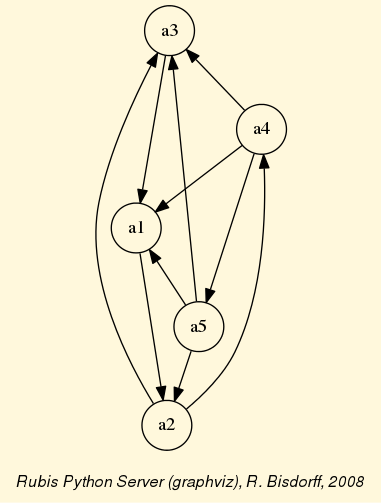
\includegraphics{cycles.png}\hfill}
\begin{description}
\item[{But, there may be many cycles appearing in a digraph, and, we may detect and enumerate all minimal chordless circuits in a Digraph instance with the \code{computeChaordlessCircuits()} method:}] \leavevmode
\begin{Verbatim}[commandchars=\\\{\}]
\PYG{g+gp}{\PYGZgt{}\PYGZgt{}\PYGZgt{} }\PYG{n}{cdg}\PYG{o}{.}\PYG{n}{computeChordlessCircuits}\PYG{p}{(}\PYG{p}{)}
\PYG{g+go}{[([\PYGZsq{}a2\PYGZsq{}, \PYGZsq{}a3\PYGZsq{}, \PYGZsq{}a1\PYGZsq{}], frozenset(\PYGZob{}\PYGZsq{}a2\PYGZsq{}, \PYGZsq{}a3\PYGZsq{}, \PYGZsq{}a1\PYGZsq{}\PYGZcb{})),}
\PYG{g+go}{ ([\PYGZsq{}a2\PYGZsq{}, \PYGZsq{}a4\PYGZsq{}, \PYGZsq{}a5\PYGZsq{}], frozenset(\PYGZob{}\PYGZsq{}a2\PYGZsq{}, \PYGZsq{}a5\PYGZsq{}, \PYGZsq{}a4\PYGZsq{}\PYGZcb{})),}
\PYG{g+go}{ ([\PYGZsq{}a2\PYGZsq{}, \PYGZsq{}a4\PYGZsq{}, \PYGZsq{}a1\PYGZsq{}], frozenset(\PYGZob{}\PYGZsq{}a2\PYGZsq{}, \PYGZsq{}a1\PYGZsq{}, \PYGZsq{}a4\PYGZsq{}\PYGZcb{}))]}
\end{Verbatim}

\end{description}

Condorcet's approach for determining the winner of an election is hence not decisive in all circomstances and we need to exploit more sophisticated approaches for finding the winner of the election on the basis of the majority margins of the given linear ballots (see {\hyperref[tutorial:bis-2008]{{[}BIS-2008{]}}}).

Many more tools for exploiting voting results are available, see the thechnical documentation of the {\hyperref[techDoc:votingdigraphs-label]{\emph{votingDigraphs module}}}.

Back to {\hyperref[tutorial:tutorial-label]{\emph{Content}}}


\subsection{Working with the \texttt{outrankingDigraphs} module}
\label{tutorial:outrankingdigraphs-tutorial-label}\label{tutorial:working-with-the-outrankingdigraphs-module}
See also the technical documentation of the {\hyperref[techDoc:outrankingdigraphs-label]{\emph{outrankingDigraphs module}}}.


\subsubsection{Structure of an outranking digraph}
\label{tutorial:structure-of-an-outranking-digraph}
In this \emph{Digraph3} module, the root \code{OutrankingDiraph} class provides a generic \textbf{outranking digraph model}. A given object of this class consists in:
\begin{enumerate}
\item {} 
a potential set of decision \textbf{actions} : a dictionary describing the potential decision actions or alternatives with `name' and `comment' attributes,

\item {} 
a coherent family of \textbf{criteria}: a dictionary of criteria functions used for measuring the performance of each potential decision action with respect to the preference dimension captured by each criterion,

\item {} 
the \textbf{evaluations}: a dictionary of performance evaluations for each decision action or alternative on each criterion function.

\item {} 
the digraph \textbf{valuationdomain}, a dictionary with three entries: the \emph{minimum} (-100, means certainly no link), the \emph{median} (0, means missing information) and the \emph{maximum} characteristic value (+100, means certainly a link),

\item {} 
the \textbf{outranking relation} : a double dictionary defined on the Cartesian product of the set of decision alternatives capturing the credibility of the pairwise \emph{outranking situation} computed on the basis of the performance differences observed between couples of decision alternatives on the given family if criteria functions.

\end{enumerate}
\begin{description}
\item[{With the help of the \code{RandomBipolarOutrankingDigraph} class (of type \code{BipolarOutrankingDigraph}) , let us generate for illustration a random bipolar outranking digraph consisting of 7 decision actions denoted \emph{a01}, \emph{a02}, ..., \emph{a07}:}] \leavevmode
\begin{Verbatim}[commandchars=\\\{\}]
\PYG{g+gp}{\PYGZgt{}\PYGZgt{}\PYGZgt{} }\PYG{k+kn}{from} \PYG{n+nn}{outrankingDigraphs} \PYG{k+kn}{import} \PYG{o}{*}
\PYG{g+gp}{\PYGZgt{}\PYGZgt{}\PYGZgt{} }\PYG{n}{odg} \PYG{o}{=} \PYG{n}{RandomBipolarOutrankingDigraph}\PYG{p}{(}\PYG{p}{)}
\PYG{g+gp}{\PYGZgt{}\PYGZgt{}\PYGZgt{} }\PYG{n}{odg}\PYG{o}{.}\PYG{n}{showActions}\PYG{p}{(}\PYG{p}{)}
\PYG{g+go}{*\PYGZhy{}\PYGZhy{}\PYGZhy{}\PYGZhy{}\PYGZhy{} show digraphs actions \PYGZhy{}\PYGZhy{}\PYGZhy{}\PYGZhy{}\PYGZhy{}\PYGZhy{}\PYGZhy{}\PYGZhy{}\PYGZhy{}\PYGZhy{}\PYGZhy{}\PYGZhy{}\PYGZhy{}\PYGZhy{}*}
\PYG{g+go}{key:  a01}
\PYG{g+go}{name:       random decision action}
\PYG{g+go}{comment:    RandomPerformanceTableau() generated.}
\PYG{g+go}{key:  a02}
\PYG{g+go}{name:       random decision action}
\PYG{g+go}{comment:    RandomPerformanceTableau() generated.}
\PYG{g+gp}{...}
\PYG{g+gp}{...}
\PYG{g+go}{key:  a07}
\PYG{g+go}{name:       random decision action}
\PYG{g+go}{comment:    RandomPerformanceTableau() generated.}
\PYG{g+gp}{\PYGZgt{}\PYGZgt{}\PYGZgt{} }\PYG{o}{.}\PYG{o}{.}\PYG{o}{.}
\end{Verbatim}

\item[{In this example we consider furthermore a family of seven equisignificant cardinal criteria functions \emph{g01}, \emph{g02}, ..., \emph{g07}, measuring the performance of each alternative on a rational scale form 0.0 to 100.00. In order to capture the evaluation's uncertainty and imprecision, each criterion function \emph{g1} to \emph{g7} admits three performance discrimination thresholds of 10, 20 and 80 pts for warranting respectively any indifference, preference and veto situations:}] \leavevmode
\begin{Verbatim}[commandchars=\\\{\}]
\PYG{g+gp}{\PYGZgt{}\PYGZgt{}\PYGZgt{} }\PYG{n}{odg}\PYG{o}{.}\PYG{n}{showCriteria}\PYG{p}{(}\PYG{p}{)}
\PYG{g+go}{*\PYGZhy{}\PYGZhy{}\PYGZhy{}\PYGZhy{}  criteria \PYGZhy{}\PYGZhy{}\PYGZhy{}\PYGZhy{}\PYGZhy{}*}
\PYG{g+go}{g01 \PYGZsq{}digraphs.RandomPerformanceTableau() instance\PYGZsq{}}
\PYG{g+go}{  Scale = [0.0, 100.0]}
\PYG{g+go}{  Weight = 3.0}
\PYG{g+go}{  Threshold pref : 20.00 + 0.00x ; percentile:  0.28}
\PYG{g+go}{  Threshold ind : 10.00 + 0.00x ; percentile:  0.095}
\PYG{g+go}{  Threshold veto : 80.00 + 0.00x ; percentile:  1.0}
\PYG{g+go}{g02 \PYGZsq{}digraphs.RandomPerformanceTableau() instance\PYGZsq{}}
\PYG{g+go}{  Scale = [0.0, 100.0]}
\PYG{g+go}{  Weight = 3.0}
\PYG{g+go}{  Threshold pref : 20.00 + 0.00x ; percentile:  0.33}
\PYG{g+go}{  Threshold ind : 10.00 + 0.00x ; percentile:  0.19}
\PYG{g+go}{  Threshold veto : 80.00 + 0.00x ; percentile:  0.95}
\PYG{g+gp}{...}
\PYG{g+gp}{...}
\PYG{g+go}{g07 \PYGZsq{}digraphs.RandomPerformanceTableau() instance\PYGZsq{}}
\PYG{g+go}{  Scale = [0.0, 100.0]}
\PYG{g+go}{  Weight = 10.0}
\PYG{g+go}{  Threshold pref : 20.00 + 0.00x ; percentile:  0.476}
\PYG{g+go}{  Threshold ind : 10.00 + 0.00x ; percentile:  0.238}
\PYG{g+go}{  Threshold veto : 80.00 + 0.00x ; percentile:  1.0}
\end{Verbatim}

\item[{The performance evaluations of each decision alternative on each criterion are gathered in a \emph{performance tableau}:}] \leavevmode
\begin{Verbatim}[commandchars=\\\{\}]
\PYG{g+gp}{\PYGZgt{}\PYGZgt{}\PYGZgt{} }\PYG{n}{odg}\PYG{o}{.}\PYG{n}{showPerformanceTableau}\PYG{p}{(}\PYG{p}{)}
\PYG{g+go}{*\PYGZhy{}\PYGZhy{}\PYGZhy{}\PYGZhy{}  performance tableau \PYGZhy{}\PYGZhy{}\PYGZhy{}\PYGZhy{}\PYGZhy{}*}
\PYG{g+go}{criteria \textbar{}  \PYGZsq{}a01\PYGZsq{}   \PYGZsq{}a02\PYGZsq{}   \PYGZsq{}a03\PYGZsq{}   \PYGZsq{}a04\PYGZsq{}   \PYGZsq{}a05\PYGZsq{}   \PYGZsq{}a06\PYGZsq{}   \PYGZsq{}a07\PYGZsq{}}
\PYG{g+go}{\PYGZhy{}\PYGZhy{}\PYGZhy{}\PYGZhy{}\PYGZhy{}\PYGZhy{}\PYGZhy{}\PYGZhy{}\PYGZhy{}\textbar{}\PYGZhy{}\PYGZhy{}\PYGZhy{}\PYGZhy{}\PYGZhy{}\PYGZhy{}\PYGZhy{}\PYGZhy{}\PYGZhy{}\PYGZhy{}\PYGZhy{}\PYGZhy{}\PYGZhy{}\PYGZhy{}\PYGZhy{}\PYGZhy{}\PYGZhy{}\PYGZhy{}\PYGZhy{}\PYGZhy{}\PYGZhy{}\PYGZhy{}\PYGZhy{}\PYGZhy{}\PYGZhy{}\PYGZhy{}\PYGZhy{}\PYGZhy{}\PYGZhy{}\PYGZhy{}\PYGZhy{}\PYGZhy{}\PYGZhy{}\PYGZhy{}\PYGZhy{}\PYGZhy{}\PYGZhy{}\PYGZhy{}\PYGZhy{}\PYGZhy{}\PYGZhy{}\PYGZhy{}\PYGZhy{}\PYGZhy{}\PYGZhy{}\PYGZhy{}\PYGZhy{}\PYGZhy{}\PYGZhy{}\PYGZhy{}\PYGZhy{}\PYGZhy{}\PYGZhy{}\PYGZhy{}}
\PYG{g+go}{  \PYGZsq{}g01\PYGZsq{}  \textbar{}   9.6    48.8    21.7    37.3    81.9    48.7    87.7}
\PYG{g+go}{  \PYGZsq{}g02\PYGZsq{}  \textbar{}  90.9    11.8    96.6    41.0    34.0    53.9    46.3}
\PYG{g+go}{  \PYGZsq{}g03\PYGZsq{}  \textbar{}  97.8    46.4    83.3    30.9    61.5    85.4    82.5}
\PYG{g+go}{  \PYGZsq{}g04\PYGZsq{}  \textbar{}  40.5    43.6    53.2    17.5    38.6    21.5    67.6}
\PYG{g+go}{  \PYGZsq{}g05\PYGZsq{}  \textbar{}  33.0    40.7    96.4    55.1    46.2    58.1    52.6}
\PYG{g+go}{  \PYGZsq{}g06\PYGZsq{}  \textbar{}  47.6    19.0    92.7    55.3    51.7    26.6    40.4}
\PYG{g+go}{  \PYGZsq{}g07\PYGZsq{}  \textbar{}  41.2    64.0    87.7    71.6    57.8    59.3    34.7}
\PYG{g+gp}{\PYGZgt{}\PYGZgt{}\PYGZgt{} }\PYG{o}{.}\PYG{o}{.}\PYG{o}{.}
\end{Verbatim}

\item[{We may visualize the same performance tableau in a more colorful setting in the default system browser with the command:}] \leavevmode
\begin{Verbatim}[commandchars=\\\{\}]
\PYG{g+gp}{\PYGZgt{}\PYGZgt{}\PYGZgt{} }\PYG{n}{dog}\PYG{o}{.}\PYG{n}{showHTMLPerformanceTableau}\PYG{p}{(}\PYG{p}{)}
\PYG{g+gp}{\PYGZgt{}\PYGZgt{}\PYGZgt{} }\PYG{o}{.}\PYG{o}{.}\PYG{o}{.}
\end{Verbatim}

\end{description}

{\hfill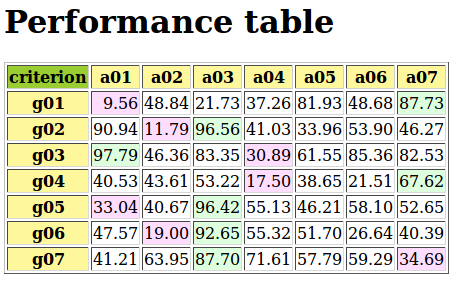
\includegraphics{tutorialPerfTab.png}\hfill}

It is worthwhile noticing that \emph{green} and \emph{red} marked evaluations indicate \emph{best}, respectively \emph{worst}, performances of an alternative on a criterion. In this example, we may hence notice that alternative \emph{a03} is in fact best performing on \emph{four} out of \emph{seven} criteria.


\subsubsection{Semantics of the bipolar valuation}
\label{tutorial:semantics-of-the-bipolar-valuation}\begin{description}
\item[{Considering the given performance tableau, the \code{BipolarOutrankingDigraph} class constructor computes the characteristic value r(x S y) of a pairwise outranking relation ``x S y'' (see {\hyperref[tutorial:bis-2013]{{[}BIS-2013{]}}}) in a default valuation domain {[}-100.0,+100.0{]} with the median value 0.0 acting as indeterminate characteristic value. The semantics of r(x S y) are the following:}] \leavevmode\begin{enumerate}
\item {} 
If r(x S y) \textgreater{} 0.0 it is more \emph{True} than \emph{False} that \emph{x outranks y}, i.e. alternative x is at least as well performing than alternative y \textbf{and} there is no considerable negative performance difference observed in disfavour of x,

\item {} 
If r(x S y) \textless{} 0.0 it is more \emph{False} than \emph{True} that \emph{x outranks y}, i.e. alternative x is \textbf{not} at least as well performing than alternative y \textbf{and} there is no considerable positive performance difference observed in favour of x,

\item {} 
If r(x S y) = 0.0 it is \emph{indeterminate} whether \emph{x outranks y or not}.

\end{enumerate}

\item[{The resulting bipolarly valued outranking relation may be inspected with the following command:}] \leavevmode
\begin{Verbatim}[commandchars=\\\{\}]
\PYG{g+gp}{\PYGZgt{}\PYGZgt{}\PYGZgt{} }\PYG{n}{odg}\PYG{o}{.}\PYG{n}{showRelationTable}\PYG{p}{(}\PYG{p}{)}
\PYG{g+go}{* \PYGZhy{}\PYGZhy{}\PYGZhy{}\PYGZhy{} Relation Table \PYGZhy{}\PYGZhy{}\PYGZhy{}\PYGZhy{}\PYGZhy{}}
\PYG{g+go}{r(x S y)\textbar{}   \PYGZsq{}a01\PYGZsq{}   \PYGZsq{}a02\PYGZsq{}   \PYGZsq{}a03\PYGZsq{}   \PYGZsq{}a04\PYGZsq{}   \PYGZsq{}a05\PYGZsq{}   \PYGZsq{}a06\PYGZsq{}   \PYGZsq{}a07\PYGZsq{}}
\PYG{g+go}{\PYGZhy{}\PYGZhy{}\PYGZhy{}\PYGZhy{}\PYGZhy{}\PYGZhy{}\PYGZhy{}\PYGZhy{}\textbar{}\PYGZhy{}\PYGZhy{}\PYGZhy{}\PYGZhy{}\PYGZhy{}\PYGZhy{}\PYGZhy{}\PYGZhy{}\PYGZhy{}\PYGZhy{}\PYGZhy{}\PYGZhy{}\PYGZhy{}\PYGZhy{}\PYGZhy{}\PYGZhy{}\PYGZhy{}\PYGZhy{}\PYGZhy{}\PYGZhy{}\PYGZhy{}\PYGZhy{}\PYGZhy{}\PYGZhy{}\PYGZhy{}\PYGZhy{}\PYGZhy{}\PYGZhy{}\PYGZhy{}\PYGZhy{}\PYGZhy{}\PYGZhy{}\PYGZhy{}\PYGZhy{}\PYGZhy{}\PYGZhy{}\PYGZhy{}\PYGZhy{}\PYGZhy{}\PYGZhy{}\PYGZhy{}\PYGZhy{}\PYGZhy{}\PYGZhy{}\PYGZhy{}\PYGZhy{}\PYGZhy{}\PYGZhy{}\PYGZhy{}\PYGZhy{}\PYGZhy{}\PYGZhy{}\PYGZhy{}\PYGZhy{}\PYGZhy{}\PYGZhy{}\PYGZhy{}\PYGZhy{}\PYGZhy{}\PYGZhy{}\PYGZhy{}\PYGZhy{}}
\PYG{g+go}{ \PYGZsq{}a01\PYGZsq{}  \textbar{}   +0.00  +29.73  \PYGZhy{}29.73  +13.51  +48.65  +40.54  +48.65}
\PYG{g+go}{ \PYGZsq{}a02\PYGZsq{}  \textbar{}  +13.51   +0.00 \PYGZhy{}100.00  +37.84  +13.51  +43.24  \PYGZhy{}37.84}
\PYG{g+go}{ \PYGZsq{}a03\PYGZsq{}  \textbar{}  +83.78 +100.00   +0.00  +91.89  +83.78  +83.78  +70.27}
\PYG{g+go}{ \PYGZsq{}a04\PYGZsq{}  \textbar{}  +24.32  +48.65  \PYGZhy{}56.76   +0.00  +24.32  +51.35  +24.32}
\PYG{g+go}{ \PYGZsq{}a05\PYGZsq{}  \textbar{}  +51.35 +100.00  \PYGZhy{}70.27  +72.97   +0.00  +51.35  +32.43}
\PYG{g+go}{ \PYGZsq{}a06\PYGZsq{}  \textbar{}  +16.22  +72.97  \PYGZhy{}51.35  +35.14  +32.43   +0.00  +37.84}
\PYG{g+go}{ \PYGZsq{}a07\PYGZsq{}  \textbar{}  +67.57  +45.95  \PYGZhy{}24.32  +27.03  +27.03  +45.95   +0.00}
\PYG{g+gp}{\PYGZgt{}\PYGZgt{}\PYGZgt{} }\PYG{n}{odg}\PYG{o}{.}\PYG{n}{valuationdomain}
\PYG{g+go}{\PYGZob{}\PYGZsq{}min\PYGZsq{}: Decimal(\PYGZsq{}\PYGZhy{}100.0\PYGZsq{}), \PYGZsq{}max\PYGZsq{}: Decimal(\PYGZsq{}100.0\PYGZsq{}), \PYGZsq{}med\PYGZsq{}: Decimal(\PYGZsq{}0.0\PYGZsq{})\PYGZcb{}}
\end{Verbatim}

\end{description}


\subsubsection{Pairwise multiple criteria comparisons}
\label{tutorial:pairwise-multiple-criteria-comparisons}\begin{description}
\item[{From above given semantics, we may consider that \emph{a01} outranks \emph{a02} (r(a01 S a02) \textgreater{} 0.0), but not \emph{a03} (r(a01 S a03) \textless{} 0.0). In order to make understandable the characteristic values shown in the relation table above, we may furthermore have a look at the pairwise multiple criteria comparison between alternatives \emph{a01} and \emph{a02}:}] \leavevmode
\begin{Verbatim}[commandchars=\\\{\}]
\PYG{g+gp}{\PYGZgt{}\PYGZgt{}\PYGZgt{} }\PYG{n}{odg}\PYG{o}{.}\PYG{n}{showPairwiseComparison}\PYG{p}{(}\PYG{l+s}{\PYGZsq{}}\PYG{l+s}{a01}\PYG{l+s}{\PYGZsq{}}\PYG{p}{,}\PYG{l+s}{\PYGZsq{}}\PYG{l+s}{a02}\PYG{l+s}{\PYGZsq{}}\PYG{p}{)}
\PYG{g+go}{*\PYGZhy{}\PYGZhy{}\PYGZhy{}\PYGZhy{}\PYGZhy{}\PYGZhy{}\PYGZhy{}\PYGZhy{}\PYGZhy{}\PYGZhy{}\PYGZhy{}\PYGZhy{}  pairwise comparison \PYGZhy{}\PYGZhy{}\PYGZhy{}\PYGZhy{}*}
\PYG{g+go}{Comparing actions : (a01, a02)}
\PYG{g+go}{crit. wght.   g(x)  g(y)    diff        \textbar{} ind     p    concord  \textbar{}}
\PYG{g+go}{\PYGZhy{}\PYGZhy{}\PYGZhy{}\PYGZhy{}\PYGZhy{}\PYGZhy{}\PYGZhy{}\PYGZhy{}\PYGZhy{}\PYGZhy{}\PYGZhy{}\PYGZhy{}\PYGZhy{}\PYGZhy{}\PYGZhy{}\PYGZhy{}\PYGZhy{}\PYGZhy{}\PYGZhy{}\PYGZhy{}\PYGZhy{}\PYGZhy{}\PYGZhy{}\PYGZhy{}\PYGZhy{}\PYGZhy{}\PYGZhy{}\PYGZhy{}\PYGZhy{}\PYGZhy{}\PYGZhy{} \PYGZhy{}\PYGZhy{}\PYGZhy{}\PYGZhy{}\PYGZhy{}\PYGZhy{}\PYGZhy{}\PYGZhy{}\PYGZhy{}\PYGZhy{}\PYGZhy{}\PYGZhy{}\PYGZhy{}\PYGZhy{}\PYGZhy{}\PYGZhy{}\PYGZhy{}\PYGZhy{}\PYGZhy{}\PYGZhy{}\PYGZhy{}\PYGZhy{}\PYGZhy{}\PYGZhy{}\PYGZhy{}\PYGZhy{}\PYGZhy{}\PYGZhy{}\PYGZhy{}\PYGZhy{}\PYGZhy{}\PYGZhy{}\PYGZhy{}}
\PYG{g+go}{g01    3.00   9.56  48.84  \PYGZhy{}39.28       \textbar{} 10.00  20.00   \PYGZhy{}3.00  \textbar{}}
\PYG{g+go}{g02    3.00  90.94  11.79  +79.15       \textbar{} 10.00  20.00   +3.00  \textbar{}}
\PYG{g+go}{g03    6.00  97.79  46.36  +51.43       \textbar{} 10.00  20.00   +6.00  \textbar{}}
\PYG{g+go}{g04    5.00  40.53  43.61   \PYGZhy{}3.08       \textbar{} 10.00  20.00   +5.00  \textbar{}}
\PYG{g+go}{g05    3.00  33.04  40.67   \PYGZhy{}7.63       \textbar{} 10.00  20.00   +3.00  \textbar{}}
\PYG{g+go}{g06    7.00  47.57  19.00  +28.57       \textbar{} 10.00  20.00   +7.00  \textbar{}}
\PYG{g+go}{g07   10.00  41.21  63.95  \PYGZhy{}22.74       \textbar{} 10.00  20.00  \PYGZhy{}10.00  \textbar{}}
\PYG{g+go}{\PYGZhy{}\PYGZhy{}\PYGZhy{}\PYGZhy{}\PYGZhy{}\PYGZhy{}\PYGZhy{}\PYGZhy{}\PYGZhy{}\PYGZhy{}\PYGZhy{}\PYGZhy{}\PYGZhy{}\PYGZhy{}\PYGZhy{}\PYGZhy{}\PYGZhy{}\PYGZhy{}\PYGZhy{}\PYGZhy{}\PYGZhy{}\PYGZhy{}\PYGZhy{}\PYGZhy{}\PYGZhy{}\PYGZhy{}\PYGZhy{}\PYGZhy{}\PYGZhy{}\PYGZhy{}\PYGZhy{}\PYGZhy{}\PYGZhy{}\PYGZhy{}\PYGZhy{}\PYGZhy{}\PYGZhy{}\PYGZhy{}\PYGZhy{}\PYGZhy{}\PYGZhy{}\PYGZhy{}\PYGZhy{}\PYGZhy{}\PYGZhy{}\PYGZhy{}\PYGZhy{}\PYGZhy{}\PYGZhy{}\PYGZhy{}\PYGZhy{}\PYGZhy{}\PYGZhy{}\PYGZhy{}\PYGZhy{}\PYGZhy{}\PYGZhy{}\PYGZhy{}\PYGZhy{}\PYGZhy{}\PYGZhy{}\PYGZhy{}\PYGZhy{}\PYGZhy{}\PYGZhy{}}
\PYG{g+go}{Valuation in range: \PYGZhy{}37.00 to +37.00; global concordance: +11.00}
\end{Verbatim}

\item[{The outranking valuation characteristic appears as \textbf{majority margin} resulting from the difference of the weights of the criteria in favor of the statement that alternative \emph{a01} is at least well performing as alternative \emph{a02}. No considerable performance difference being observed, no veto or counter.veto situation is triggered in this pairwise comparison. Such a case is, however, observed for instance when we pairwise compare the performances of alternatives \emph{a03} and \emph{a02}:}] \leavevmode
\begin{Verbatim}[commandchars=\\\{\}]
\PYG{g+gp}{\PYGZgt{}\PYGZgt{}\PYGZgt{} }\PYG{n}{odg}\PYG{o}{.}\PYG{n}{showPairwiseComparison}\PYG{p}{(}\PYG{l+s}{\PYGZsq{}}\PYG{l+s}{a03}\PYG{l+s}{\PYGZsq{}}\PYG{p}{,}\PYG{l+s}{\PYGZsq{}}\PYG{l+s}{a02}\PYG{l+s}{\PYGZsq{}}\PYG{p}{)}
\PYG{g+go}{*\PYGZhy{}\PYGZhy{}\PYGZhy{}\PYGZhy{}\PYGZhy{}\PYGZhy{}\PYGZhy{}\PYGZhy{}\PYGZhy{}\PYGZhy{}\PYGZhy{}\PYGZhy{}  pairwise comparison \PYGZhy{}\PYGZhy{}\PYGZhy{}\PYGZhy{}*}
\PYG{g+go}{Comparing actions : (a03, a02)}
\PYG{g+go}{crit.  wght.  g(x)  g(y)    diff        \textbar{} ind     p    concord  \textbar{}  v  veto/counter\PYGZhy{}}
\PYG{g+go}{\PYGZhy{}\PYGZhy{}\PYGZhy{}\PYGZhy{}\PYGZhy{}\PYGZhy{}\PYGZhy{}\PYGZhy{}\PYGZhy{}\PYGZhy{}\PYGZhy{}\PYGZhy{}\PYGZhy{}\PYGZhy{}\PYGZhy{}\PYGZhy{}\PYGZhy{}\PYGZhy{}\PYGZhy{}\PYGZhy{}\PYGZhy{}\PYGZhy{}\PYGZhy{}\PYGZhy{}\PYGZhy{}\PYGZhy{}\PYGZhy{}\PYGZhy{}\PYGZhy{}\PYGZhy{}\PYGZhy{}\PYGZhy{}\PYGZhy{}\PYGZhy{}\PYGZhy{}\PYGZhy{}\PYGZhy{}\PYGZhy{}\PYGZhy{}\PYGZhy{}\PYGZhy{}\PYGZhy{}\PYGZhy{}\PYGZhy{}\PYGZhy{}\PYGZhy{}\PYGZhy{}\PYGZhy{}\PYGZhy{}\PYGZhy{}\PYGZhy{}\PYGZhy{}\PYGZhy{}\PYGZhy{}\PYGZhy{}\PYGZhy{}\PYGZhy{}\PYGZhy{}\PYGZhy{}\PYGZhy{}\PYGZhy{}\PYGZhy{}\PYGZhy{}\PYGZhy{}\PYGZhy{}\PYGZhy{}\PYGZhy{}\PYGZhy{}\PYGZhy{}\PYGZhy{}\PYGZhy{}\PYGZhy{}\PYGZhy{}\PYGZhy{}\PYGZhy{}\PYGZhy{}\PYGZhy{}\PYGZhy{}\PYGZhy{}\PYGZhy{}\PYGZhy{}\PYGZhy{}\PYGZhy{}}
\PYG{g+go}{g01    3.00  21.73  48.84  \PYGZhy{}27.11       \textbar{} 10.00  20.00   \PYGZhy{}3.00  \textbar{}}
\PYG{g+go}{g02    3.00  96.56  11.79  +84.77       \textbar{} 10.00  20.00   +3.00  \textbar{}  80.00  +1.00}
\PYG{g+go}{g03    6.00  83.35  46.36  +36.99       \textbar{} 10.00  20.00   +6.00  \textbar{}}
\PYG{g+go}{g04    5.00  53.22  43.61   +9.61       \textbar{} 10.00  20.00   +5.00  \textbar{}}
\PYG{g+go}{g05    3.00  96.42  40.67  +55.75       \textbar{} 10.00  20.00   +3.00  \textbar{}}
\PYG{g+go}{g06    7.00  92.65  19.00  +73.65       \textbar{} 10.00  20.00   +7.00  \textbar{}}
\PYG{g+go}{g07   10.00  87.70  63.95  +23.75       \textbar{} 10.00  20.00  +10.00  \textbar{}}
\PYG{g+go}{\PYGZhy{}\PYGZhy{}\PYGZhy{}\PYGZhy{}\PYGZhy{}\PYGZhy{}\PYGZhy{}\PYGZhy{}\PYGZhy{}\PYGZhy{}\PYGZhy{}\PYGZhy{}\PYGZhy{}\PYGZhy{}\PYGZhy{}\PYGZhy{}\PYGZhy{}\PYGZhy{}\PYGZhy{}\PYGZhy{}\PYGZhy{}\PYGZhy{}\PYGZhy{}\PYGZhy{}\PYGZhy{}\PYGZhy{}\PYGZhy{}\PYGZhy{}\PYGZhy{}\PYGZhy{}\PYGZhy{}\PYGZhy{}\PYGZhy{}\PYGZhy{}\PYGZhy{}\PYGZhy{}\PYGZhy{}\PYGZhy{}\PYGZhy{}\PYGZhy{}\PYGZhy{}\PYGZhy{}\PYGZhy{}\PYGZhy{}\PYGZhy{}\PYGZhy{}\PYGZhy{}\PYGZhy{}\PYGZhy{}\PYGZhy{}\PYGZhy{}\PYGZhy{}\PYGZhy{}\PYGZhy{}\PYGZhy{}\PYGZhy{}\PYGZhy{}\PYGZhy{}\PYGZhy{}\PYGZhy{}\PYGZhy{}\PYGZhy{}\PYGZhy{}\PYGZhy{}\PYGZhy{}\PYGZhy{}\PYGZhy{}\PYGZhy{}\PYGZhy{}\PYGZhy{}\PYGZhy{}\PYGZhy{}\PYGZhy{}\PYGZhy{}\PYGZhy{}\PYGZhy{}\PYGZhy{}\PYGZhy{}\PYGZhy{}\PYGZhy{}\PYGZhy{}\PYGZhy{}\PYGZhy{}}
\PYG{g+go}{ Valuation in range: \PYGZhy{}37.00 to +37.00; global concordance: +31.00}
\PYG{g+gp}{\PYGZgt{}\PYGZgt{}\PYGZgt{} }\PYG{o}{.}\PYG{o}{.}\PYG{o}{.}
\end{Verbatim}

\end{description}

This time, we observe a considerable out-performance of \emph{a03} against \emph{a02} on criterion g02 (see second row in the relation table above). We therefore notice a positively polarised \emph{certainly confirmed} outranking situation in this case {\hyperref[tutorial:bis-2013]{{[}BIS-2013{]}}}.


\subsubsection{Recoding the valuation}
\label{tutorial:recoding-the-valuation}\begin{description}
\item[{All outranking digraphs, being of root type \code{Digraph}, inherit the methods available under this class. The characteristic valuation domain of an outranking digraph may be recoded with the \code{Digraph.recodeValutaion()} method below to the integer range {[}-37,+37{]}, i.e. plus or minus the global significance of the family of criteria considered in this example instance:}] \leavevmode
\begin{Verbatim}[commandchars=\\\{\}]
\PYG{g+gp}{\PYGZgt{}\PYGZgt{}\PYGZgt{} }\PYG{n}{odg}\PYG{o}{.}\PYG{n}{recodeValuation}\PYG{p}{(}\PYG{o}{\PYGZhy{}}\PYG{l+m+mi}{37}\PYG{p}{,}\PYG{o}{+}\PYG{l+m+mi}{37}\PYG{p}{)}
\PYG{g+gp}{\PYGZgt{}\PYGZgt{}\PYGZgt{} }\PYG{n}{odg}\PYG{o}{.}\PYG{n}{valuationdomain}\PYG{p}{[}\PYG{l+s}{\PYGZsq{}}\PYG{l+s}{hasIntegerValuation}\PYG{l+s}{\PYGZsq{}}\PYG{p}{]} \PYG{o}{=} \PYG{n+nb+bp}{True}
\PYG{g+gp}{\PYGZgt{}\PYGZgt{}\PYGZgt{} }\PYG{n}{Digraph}\PYG{o}{.}\PYG{n}{showRelationTable}\PYG{p}{(}\PYG{n}{odg}\PYG{p}{)}
\PYG{g+go}{* \PYGZhy{}\PYGZhy{}\PYGZhy{}\PYGZhy{} Relation Table \PYGZhy{}\PYGZhy{}\PYGZhy{}\PYGZhy{}\PYGZhy{}}
\PYG{g+go}{* \PYGZhy{}\PYGZhy{}\PYGZhy{}\PYGZhy{} Relation Table \PYGZhy{}\PYGZhy{}\PYGZhy{}\PYGZhy{}\PYGZhy{}}
\PYG{g+go}{  S   \textbar{} \PYGZsq{}a01\PYGZsq{}   \PYGZsq{}a02\PYGZsq{}   \PYGZsq{}a03\PYGZsq{}  \PYGZsq{}a04\PYGZsq{}   \PYGZsq{}a05\PYGZsq{}   \PYGZsq{}a06\PYGZsq{}   \PYGZsq{}a07\PYGZsq{}}
\PYG{g+go}{\PYGZhy{}\PYGZhy{}\PYGZhy{}\PYGZhy{}\PYGZhy{}\textbar{}\PYGZhy{}\PYGZhy{}\PYGZhy{}\PYGZhy{}\PYGZhy{}\PYGZhy{}\PYGZhy{}\PYGZhy{}\PYGZhy{}\PYGZhy{}\PYGZhy{}\PYGZhy{}\PYGZhy{}\PYGZhy{}\PYGZhy{}\PYGZhy{}\PYGZhy{}\PYGZhy{}\PYGZhy{}\PYGZhy{}\PYGZhy{}\PYGZhy{}\PYGZhy{}\PYGZhy{}\PYGZhy{}\PYGZhy{}\PYGZhy{}\PYGZhy{}\PYGZhy{}\PYGZhy{}\PYGZhy{}\PYGZhy{}\PYGZhy{}\PYGZhy{}\PYGZhy{}\PYGZhy{}\PYGZhy{}\PYGZhy{}\PYGZhy{}\PYGZhy{}\PYGZhy{}\PYGZhy{}\PYGZhy{}\PYGZhy{}\PYGZhy{}\PYGZhy{}\PYGZhy{}\PYGZhy{}\PYGZhy{}\PYGZhy{}\PYGZhy{}\PYGZhy{}\PYGZhy{}\PYGZhy{}\PYGZhy{}\PYGZhy{}\PYGZhy{}\PYGZhy{}\PYGZhy{}\PYGZhy{}}
\PYG{g+go}{\PYGZsq{}a01\PYGZsq{} \textbar{}    0     +11     \PYGZhy{}11     +5     +17     +14     +17}
\PYG{g+go}{\PYGZsq{}a02\PYGZsq{} \textbar{}   +5       0     \PYGZhy{}37    +13      +5     +15     \PYGZhy{}14}
\PYG{g+go}{\PYGZsq{}a03\PYGZsq{} \textbar{}  +31     +37       0    +34     +31     +31     +26}
\PYG{g+go}{\PYGZsq{}a04\PYGZsq{} \textbar{}   +9     +18     \PYGZhy{}21      0      +9     +19      +9}
\PYG{g+go}{\PYGZsq{}a05\PYGZsq{} \textbar{}  +19     +37     \PYGZhy{}26    +27       0     +19     +12}
\PYG{g+go}{\PYGZsq{}a06\PYGZsq{} \textbar{}   +6     +27     \PYGZhy{}19    +13     +12       0     +14}
\PYG{g+go}{\PYGZsq{}a07\PYGZsq{} \textbar{}  +25     +17      \PYGZhy{}9     +9      +9     +17       0}
\PYG{g+go}{Valuation domain:  \PYGZob{}\PYGZsq{}hasIntegerValuation\PYGZsq{}: True, \PYGZsq{}min\PYGZsq{}: Decimal(\PYGZsq{}\PYGZhy{}37\PYGZsq{}),}
\PYG{g+go}{                    \PYGZsq{}max\PYGZsq{}: Decimal(\PYGZsq{}37\PYGZsq{}), \PYGZsq{}med\PYGZsq{}: Decimal(\PYGZsq{}0.000\PYGZsq{})\PYGZcb{}}
\PYG{g+gp}{\PYGZgt{}\PYGZgt{}\PYGZgt{} }\PYG{o}{.}\PYG{o}{.}\PYG{o}{.}
\end{Verbatim}

\end{description}

\begin{notice}{note}{Note:}
Notice that the reflexive self comparison characteristic r(x S x) is set by default to the median indeterminate valuation value 0; the reflexive terms of binary relation being generally ignored in most of the \code{Digraph3} resources.
\end{notice}


\subsubsection{Strict outranking via the codual digraph}
\label{tutorial:strict-outranking-via-the-codual-digraph}\begin{description}
\item[{From the theory {\hyperref[tutorial:bis-2013]{{[}BIS-2013{]}}} we know that the bipolarly outranking relation is \textbf{weakly complete}, i.e. if r(x S y) \textless{} 0.0 then r(y S x) \textgreater{}= 0.0 . From this property follows that the bipolarly valued outranking relation verifies the coduality principle: the dual (-) of the converse (\textasciitilde{}) of the outranking relation corresponds to its strict outranking part. We may visualize the codual (strict) outranking digraph with a graphviz drawing \footnotemark[1]:}] \leavevmode
\begin{Verbatim}[commandchars=\\\{\}]
\PYG{g+gp}{\PYGZgt{}\PYGZgt{}\PYGZgt{} }\PYG{n}{cdodg} \PYG{o}{=} \PYG{o}{\PYGZhy{}}\PYG{p}{(}\PYG{o}{\PYGZti{}}\PYG{n}{odg}\PYG{p}{)}
\PYG{g+gp}{\PYGZgt{}\PYGZgt{}\PYGZgt{} }\PYG{n}{cdodg}\PYG{o}{.}\PYG{n}{exportGraphViz}\PYG{p}{(}\PYG{l+s}{\PYGZsq{}}\PYG{l+s}{codualOdg}\PYG{l+s}{\PYGZsq{}}\PYG{p}{)}
\PYG{g+go}{*\PYGZhy{}\PYGZhy{}\PYGZhy{}\PYGZhy{} exporting a dot file for GraphViz tools \PYGZhy{}\PYGZhy{}\PYGZhy{}\PYGZhy{}\PYGZhy{}\PYGZhy{}\PYGZhy{}\PYGZhy{}\PYGZhy{}*}
\PYG{g+go}{Exporting to codualOdg.dot}
\PYG{g+go}{dot \PYGZhy{}Grankdir=BT \PYGZhy{}Tpng codualOdg.dot \PYGZhy{}o codualOdg.png}
\PYG{g+gp}{\PYGZgt{}\PYGZgt{}\PYGZgt{} }\PYG{o}{.}\PYG{o}{.}\PYG{o}{.}
\end{Verbatim}

\end{description}

{\hfill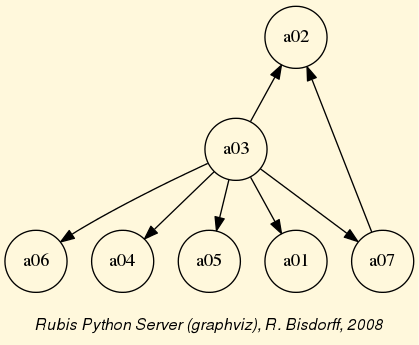
\includegraphics{codualOdg.png}\hfill}

It becomes readily clear now from the picture above that alternative \emph{a03} strictly outranks in fact all the other alternatives. Hence, \emph{a03} appears as \textbf{Condorcet winner} and may be recommended as \emph{best decision action} in this illustrative preference modelling exercise.


\subsubsection{XMCDA 2.0 storage}
\label{tutorial:xmcda-2-0-storage}\begin{description}
\item[{As with all Digraph instances, it is possible to store permanently a copy of the outranking digraph \emph{odg}. As its outranking relation is automatically generated by the \code{BipolarOutrankingDigraph} class constructor on the basis of a given performance tableau, it is sufficient to save only the latter. For this purpose we are using the \href{http://www.decision-deck.org/xmcda/}{XMCDA 2.00} XML encoding scheme of MCDA data, as provided by the Decision Deck Project (see \href{http://www.decision-deck.org/}{http://www.decision-deck.org/}):}] \leavevmode
\begin{Verbatim}[commandchars=\\\{\}]
\PYG{g+gp}{\PYGZgt{}\PYGZgt{}\PYGZgt{} }\PYG{n}{PerformanceTableau}\PYG{o}{.}\PYG{n}{saveXMCDA2}\PYG{p}{(}\PYG{n}{odg}\PYG{p}{,}\PYG{l+s}{\PYGZsq{}}\PYG{l+s}{tutorialPerfTab}\PYG{l+s}{\PYGZsq{}}\PYG{p}{)}
\PYG{g+go}{*\PYGZhy{}\PYGZhy{}\PYGZhy{}\PYGZhy{}\PYGZhy{} saving performance tableau in XMCDA 2.0 format  \PYGZhy{}\PYGZhy{}\PYGZhy{}\PYGZhy{}\PYGZhy{}\PYGZhy{}\PYGZhy{}\PYGZhy{}\PYGZhy{}\PYGZhy{}\PYGZhy{}\PYGZhy{}\PYGZhy{}*}
\PYG{g+go}{File: tutorialPerfTab.xml saved !}
\PYG{g+gp}{\PYGZgt{}\PYGZgt{}\PYGZgt{} }\PYG{o}{.}\PYG{o}{.}\PYG{o}{.}
\end{Verbatim}

\item[{The resulting XML file my be visualized in a browser window (other than Chrome or Chromium)  with a corresponding XMCDA style sheet (see here). Hitting \code{Ctrl U} in Firefox will open a browser window showing the underlying xml encoded raw text. It is thus possible to easily edit and update as needed a given performance tableau instance. Reinstantiating again a corresponding updated \emph{odg} object goes like follow:}] \leavevmode
\begin{Verbatim}[commandchars=\\\{\}]
\PYG{g+gp}{\PYGZgt{}\PYGZgt{}\PYGZgt{} }\PYG{n}{pt} \PYG{o}{=} \PYG{n}{XMCDA2PerformanceTableau}\PYG{p}{(}\PYG{l+s}{\PYGZsq{}}\PYG{l+s}{tutorialPerfTab}\PYG{l+s}{\PYGZsq{}}\PYG{p}{)}
\PYG{g+gp}{\PYGZgt{}\PYGZgt{}\PYGZgt{} }\PYG{n}{odg} \PYG{o}{=} \PYG{n}{BipolarOutrankingDigraph}\PYG{p}{(}\PYG{n}{pt}\PYG{p}{)}
\PYG{g+gp}{\PYGZgt{}\PYGZgt{}\PYGZgt{} }\PYG{n}{odg}\PYG{o}{.}\PYG{n}{showRelationTable}\PYG{p}{(}\PYG{p}{)}
\PYG{g+go}{* \PYGZhy{}\PYGZhy{}\PYGZhy{}\PYGZhy{} Relation Table \PYGZhy{}\PYGZhy{}\PYGZhy{}\PYGZhy{}\PYGZhy{}}
\PYG{g+go}{  S   \textbar{}  \PYGZsq{}a01\PYGZsq{}     \PYGZsq{}a02\PYGZsq{}   \PYGZsq{}a03\PYGZsq{}   \PYGZsq{}a04\PYGZsq{}   \PYGZsq{}a05\PYGZsq{}   \PYGZsq{}a06\PYGZsq{}   \PYGZsq{}a07\PYGZsq{}}
\PYG{g+go}{\PYGZhy{}\PYGZhy{}\PYGZhy{}\PYGZhy{}\PYGZhy{}\PYGZhy{}\textbar{}\PYGZhy{}\PYGZhy{}\PYGZhy{}\PYGZhy{}\PYGZhy{}\PYGZhy{}\PYGZhy{}\PYGZhy{}\PYGZhy{}\PYGZhy{}\PYGZhy{}\PYGZhy{}\PYGZhy{}\PYGZhy{}\PYGZhy{}\PYGZhy{}\PYGZhy{}\PYGZhy{}\PYGZhy{}\PYGZhy{}\PYGZhy{}\PYGZhy{}\PYGZhy{}\PYGZhy{}\PYGZhy{}\PYGZhy{}\PYGZhy{}\PYGZhy{}\PYGZhy{}\PYGZhy{}\PYGZhy{}\PYGZhy{}\PYGZhy{}\PYGZhy{}\PYGZhy{}\PYGZhy{}\PYGZhy{}\PYGZhy{}\PYGZhy{}\PYGZhy{}\PYGZhy{}\PYGZhy{}\PYGZhy{}\PYGZhy{}\PYGZhy{}\PYGZhy{}\PYGZhy{}\PYGZhy{}\PYGZhy{}\PYGZhy{}\PYGZhy{}\PYGZhy{}\PYGZhy{}\PYGZhy{}\PYGZhy{}\PYGZhy{}\PYGZhy{}\PYGZhy{}\PYGZhy{}\PYGZhy{}}
\PYG{g+go}{\PYGZsq{}a01\PYGZsq{} \textbar{}   +0.00   +29.73  \PYGZhy{}29.73  +13.51  +48.65  +40.54  +48.65}
\PYG{g+go}{\PYGZsq{}a02\PYGZsq{} \textbar{}   +13.51  +0.00  \PYGZhy{}100.00  +37.84  +13.51  +43.24  \PYGZhy{}37.84}
\PYG{g+go}{\PYGZsq{}a03\PYGZsq{} \textbar{}   +83.78  +100.00  +0.00  +91.89  +83.78  +83.78  +70.27}
\PYG{g+go}{\PYGZsq{}a04\PYGZsq{} \textbar{}   +24.32  +48.65  \PYGZhy{}56.76   +0.00  +24.32  +51.35  +24.32}
\PYG{g+go}{\PYGZsq{}a05\PYGZsq{} \textbar{}   +51.35  +100.00  \PYGZhy{}70.27  +72.97  +0.00  +51.35  +32.43}
\PYG{g+go}{\PYGZsq{}a06\PYGZsq{} \textbar{}   +16.22  +72.97  \PYGZhy{}51.35  +35.14  +32.43   +0.00  +37.84}
\PYG{g+go}{\PYGZsq{}a07\PYGZsq{} \textbar{}   +67.57  +45.95  \PYGZhy{}24.32  +27.03  +27.03  +45.95   +0.00}
\PYG{g+gp}{\PYGZgt{}\PYGZgt{}\PYGZgt{} }\PYG{o}{.}\PYG{o}{.}\PYG{o}{.}
\end{Verbatim}

\end{description}

We recover the original bipolarly valued outranking characteristics, and we may restart again the preference modelling process.

Many more tools for exploiting bipolarly valued outranking digraphs are available in the Digraph3 resources (see the thechnical documentation of the {\hyperref[techDoc:outrankingdigraphs-label]{\emph{outrankingDigraphs module}}} and the {\hyperref[techDoc:perftabs-label]{\emph{perfTabs module}}}).

Back to {\hyperref[tutorial:tutorial-label]{\emph{Content}}}


\subsection{Links and appendices}
\label{tutorial:links-and-appendices}

\subsubsection{Documents}
\label{tutorial:documents}\begin{itemize}
\item {} 
Introduction

\item {} 
Reference manual

\item {} 
Tutorial

\end{itemize}


\subsubsection{Indices and tables}
\label{tutorial:indices-and-tables}\begin{itemize}
\item {} 
\emph{genindex}

\item {} 
\emph{modindex}

\item {} 
\emph{search}

\end{itemize}


\subsubsection{References}
\label{tutorial:references}

\subsubsection{Footnotes}
\label{tutorial:footnotes}

\section{Technical Reference of the Digraph3 modules}
\label{techDoc::doc}\label{techDoc:technical-reference-of-the-digraph3-modules}\begin{quote}\begin{description}
\item[{Author}] \leavevmode
Raymond Bisdorff, University of Luxembourg FSTC/CSC

\item[{Version}] \leavevmode
Revision: Python 3.4

\item[{Copyright}] \leavevmode\begin{enumerate}
\setcounter{enumi}{17}
\item {} 
Bisdorff 2013-2014

\end{enumerate}

\end{description}\end{quote}


\subsection{Introduction}
\label{techDoc:introduction}\label{techDoc:technical-label}
\textbf{Dowloading the Digraph3 ressources}

Two downlaod options are given:

1. Either (easiest under Linux or Mac OS-X), by using a subversion client::
..\$svn co \href{http://leopold-loewenheim.uni.lu/svn/repos/Digraph3}{http://leopold-loewenheim.uni.lu/svn/repos/Digraph3}

2. Or, download and extract the latest distribution tar.gz archive::
\href{http://leopold-loewenheim.uni.lu/svn/repos/Digraph3/dist/digraphs-Python3-xxx.tar.gz}{http://leopold-loewenheim.uni.lu/svn/repos/Digraph3/dist/digraphs-Python3-xxx.tar.gz}

Developping the Rubis decision support methodology is an ongoing research project of Raymond Bisdorff \textless{}\href{http://charles-sanders-peirce.uni.lu/bisdorff/}{http://charles-sanders-peirce.uni.lu/bisdorff/}\textgreater{}, University of Luxembourg.

To be fully functional, the Digraph3 resources mainly need the \href{http://graphviz.org}{graphviz} tools and the \href{http://www.r-project.org}{R statistics resources} to be installed. When exploring digraph isomorphisms, the \href{http://www.cs.sunysb.edu/~algorith/implement/nauty/implement.shtml}{nauty} isomorphism testing program is required. two specific criteria and actions clustering methods of the Digraph class furthermore require the \href{http://leopold-loewenheim.uni.lu/svn/repos/Calmat/}{calmat} matrix computing resource to be installed.

\textbf{Organisation of the Digraph3 python3 source code}

The Digraph3 source code is split into several interdependent modules, where the \code{digraphs} module is the master source.
\begin{itemize}
\item {} \begin{description}
\item[{{\hyperref[techDoc:digraphs-label]{\emph{digraphs module}}}}] \leavevmode
main part of the Digraph3 source code with the root Digraph class;

\end{description}

\item {} \begin{description}
\item[{{\hyperref[techDoc:graphs-label]{\emph{graphs module}}}}] \leavevmode
specialization for undirected graphs with the root Graph class and a brigde to the \code{digraphs} module resources;

\end{description}

\item {} \begin{description}
\item[{{\hyperref[techDoc:outrankingdigraphs-label]{\emph{outrankingDigraphs module}}}}] \leavevmode
new Python3 versioned root OutrankingDigraph class and specializations;

\end{description}

\item {} \begin{description}
\item[{{\hyperref[techDoc:perftabs-label]{\emph{perfTabs module}}}}] \leavevmode
everything needed for handling Multiple Criteria Decision Aid performance tableaux with root PerformaceTableau class;

\end{description}

\item {} \begin{description}
\item[{{\hyperref[techDoc:votingdigraphs-label]{\emph{votingDigraphs module}}}}] \leavevmode
additional classes and methods for computing election results with main LinearVotingProfile class;

\end{description}

\item {} \begin{description}
\item[{{\hyperref[techDoc:sortingdigraphs-label]{\emph{sortingDigraphs module}}}}] \leavevmode
additional tools for solving sorting problems with the root SortingDigraph class;

\end{description}

\item {} \begin{description}
\item[{{\hyperref[techDoc:linearorders-label]{\emph{linearOrders module}}}}] \leavevmode
additional tools for solving linearly ranking problems with the root LinearOrder class;

\end{description}

\item {} \begin{description}
\item[{{\hyperref[techDoc:weakorders-label]{\emph{weakOrders module}}}}] \leavevmode
additional tools for solving ranking by choosing problems with root WeakOrder class.

\end{description}

\end{itemize}


\subsection{digraphs module}
\label{techDoc:digraphs-label}\label{techDoc:digraphs-module}
A tutorial with coding examples is available here: {\hyperref[tutorial:digraphs-tutorial-label]{\emph{Working with the digraphs module}}}
\phantomsection\label{techDoc:module-digraphs}\index{digraphs (module)}\index{AsymmetricPartialDigraph (class in digraphs)}

\begin{fulllineitems}
\phantomsection\label{techDoc:digraphs.AsymmetricPartialDigraph}\pysiglinewithargsret{\strong{class }\code{digraphs.}\bfcode{AsymmetricPartialDigraph}}{\emph{digraph}}{}
Bases: {\hyperref[techDoc:digraphs.Digraph]{\code{digraphs.Digraph}}}

Renders the asymmetric part of a Digraph instance

\begin{notice}{warning}{Warning:}
Note that the non asymmetric pairs are all put to the median indeterminate
characteristic value!
\end{notice}

\end{fulllineitems}

\index{CSVDigraph (class in digraphs)}

\begin{fulllineitems}
\phantomsection\label{techDoc:digraphs.CSVDigraph}\pysiglinewithargsret{\strong{class }\code{digraphs.}\bfcode{CSVDigraph}}{\emph{fileName='temp'}, \emph{valuationMin=-1}, \emph{valuationMax=1}}{}
Bases: {\hyperref[techDoc:digraphs.Digraph]{\code{digraphs.Digraph}}}

Specialization of the general Digraph class for reading
stored csv formatted digraphs. Using the inbuilt module csv.
\begin{description}
\item[{Param:}] \leavevmode
fileName (without the extension .csv).

\end{description}
\index{showAll() (digraphs.CSVDigraph method)}

\begin{fulllineitems}
\phantomsection\label{techDoc:digraphs.CSVDigraph.showAll}\pysiglinewithargsret{\bfcode{showAll}}{}{}
\end{fulllineitems}


\end{fulllineitems}

\index{CirculantDigraph (class in digraphs)}

\begin{fulllineitems}
\phantomsection\label{techDoc:digraphs.CirculantDigraph}\pysiglinewithargsret{\strong{class }\code{digraphs.}\bfcode{CirculantDigraph}}{\emph{order=7, valuationdomain=\{`max': Decimal(`1.0'), `min': Decimal(`-1.0')\}, circulants={[}-1, 1{]}}}{}
Bases: {\hyperref[techDoc:digraphs.Digraph]{\code{digraphs.Digraph}}}
\begin{description}
\item[{Parameters:}] \leavevmode
\begin{DUlineblock}{0em}
\item[] order \textgreater{} 0;
\item[] valuationdomain =\{`min':m, `max':M\};
\item[] circulant connections = list of positive
and/or negative circular shifts of value 1 to n.
\end{DUlineblock}

\end{description}

Specialization of the general Digraph class for generating
temporary circulant digraphs
\begin{description}
\item[{Default instantiation C\_7:}] \leavevmode
\begin{DUlineblock}{0em}
\item[] order = 7,
\item[] valuationdomain = \{`min':-1.0,'max':1.0\},
\item[] circulants = {[}-1,1{]}.
\end{DUlineblock}

\end{description}
\index{showShort() (digraphs.CirculantDigraph method)}

\begin{fulllineitems}
\phantomsection\label{techDoc:digraphs.CirculantDigraph.showShort}\pysiglinewithargsret{\bfcode{showShort}}{}{}
\end{fulllineitems}


\end{fulllineitems}

\index{CoDualDigraph (class in digraphs)}

\begin{fulllineitems}
\phantomsection\label{techDoc:digraphs.CoDualDigraph}\pysiglinewithargsret{\strong{class }\code{digraphs.}\bfcode{CoDualDigraph}}{\emph{other}, \emph{Debug=False}}{}
Bases: {\hyperref[techDoc:digraphs.Digraph]{\code{digraphs.Digraph}}}

Instantiates the associated codual digraph from
a given Digraph called other.

Instantiates as other.\_\_class\_\_ !

Copies the case given the description, the criteria
and the evaluation dictionary into self.

\end{fulllineitems}

\index{CocaDigraph (class in digraphs)}

\begin{fulllineitems}
\phantomsection\label{techDoc:digraphs.CocaDigraph}\pysiglinewithargsret{\strong{class }\code{digraphs.}\bfcode{CocaDigraph}}{\emph{digraph=None}, \emph{Cpp=False}, \emph{Piping=False}, \emph{Comments=False}}{}
Bases: {\hyperref[techDoc:digraphs.Digraph]{\code{digraphs.Digraph}}}
\begin{description}
\item[{Parameters:}] \leavevmode
Stored or memory resident digraph instance.

\end{description}

Specialization of general Digraph class for instantiation
of chordless odd circuits augmented digraphs.
\index{addCircuits() (digraphs.CocaDigraph method)}

\begin{fulllineitems}
\phantomsection\label{techDoc:digraphs.CocaDigraph.addCircuits}\pysiglinewithargsret{\bfcode{addCircuits}}{\emph{Comments=False}}{}
Augmenting self with self.circuits.

\end{fulllineitems}

\index{closureChordlessOddCircuits() (digraphs.CocaDigraph method)}

\begin{fulllineitems}
\phantomsection\label{techDoc:digraphs.CocaDigraph.closureChordlessOddCircuits}\pysiglinewithargsret{\bfcode{closureChordlessOddCircuits}}{\emph{Cpp=False}, \emph{Piping=False}, \emph{Comments=False}}{}
Closure of chordless odd circuits extraction.

\end{fulllineitems}

\index{showCircuits() (digraphs.CocaDigraph method)}

\begin{fulllineitems}
\phantomsection\label{techDoc:digraphs.CocaDigraph.showCircuits}\pysiglinewithargsret{\bfcode{showCircuits}}{}{}
show methods for chordless odd circuits in CocaGraph

\end{fulllineitems}

\index{showComponents() (digraphs.CocaDigraph method)}

\begin{fulllineitems}
\phantomsection\label{techDoc:digraphs.CocaDigraph.showComponents}\pysiglinewithargsret{\bfcode{showComponents}}{}{}
\end{fulllineitems}


\end{fulllineitems}

\index{CoceDigraph (class in digraphs)}

\begin{fulllineitems}
\phantomsection\label{techDoc:digraphs.CoceDigraph}\pysiglinewithargsret{\strong{class }\code{digraphs.}\bfcode{CoceDigraph}}{\emph{digraph=None}, \emph{Cpp=False}, \emph{Piping=False}, \emph{Comments=False}, \emph{Debug=False}}{}
Bases: {\hyperref[techDoc:digraphs.Digraph]{\code{digraphs.Digraph}}}
\begin{description}
\item[{Parameters:}] \leavevmode
Stored or memory resident digraph instance.

\end{description}

Specialization of general Digraph class for instantiation
of chordless odd circuits eliminated digraphs.
\index{iterateCocElimination() (digraphs.CoceDigraph method)}

\begin{fulllineitems}
\phantomsection\label{techDoc:digraphs.CoceDigraph.iterateCocElimination}\pysiglinewithargsret{\bfcode{iterateCocElimination}}{\emph{Comments=True}, \emph{Debug=False}}{}
Eliminates all chordless odd circuits with rising valuation cut levels.
Renders a tuple (level,polarisedDigraph) where level is the
necessary bipolar cut level for eliminating all chordless odd circuits,
and polarisedDigraph is the resulting digraph instance.
Renders (None,None) if no chordless odd circuit is detected.

\end{fulllineitems}


\end{fulllineitems}

\index{CompleteDigraph (class in digraphs)}

\begin{fulllineitems}
\phantomsection\label{techDoc:digraphs.CompleteDigraph}\pysiglinewithargsret{\strong{class }\code{digraphs.}\bfcode{CompleteDigraph}}{\emph{order=5}, \emph{valuationdomain=(-1.0}, \emph{1.0)}}{}
Bases: {\hyperref[techDoc:digraphs.Digraph]{\code{digraphs.Digraph}}}
\begin{description}
\item[{Parameters:}] \leavevmode
order \textgreater{} 0; valuationdomain=(Min,Max).

\end{description}

Specialization of the general Digraph class for generating
temporary complete graphs of order 5 in \{-1,0,1\} by default.

\end{fulllineitems}

\index{ConverseDigraph (class in digraphs)}

\begin{fulllineitems}
\phantomsection\label{techDoc:digraphs.ConverseDigraph}\pysiglinewithargsret{\strong{class }\code{digraphs.}\bfcode{ConverseDigraph}}{\emph{other}}{}
Bases: {\hyperref[techDoc:digraphs.Digraph]{\code{digraphs.Digraph}}}

Instantiates the associated converse orreciprocal version from
a given Digraph called other.

Instantiates as other.\_\_class\_\_ !

Copies the case given the description, the criteria
and the evaluation dictionary into self.

\end{fulllineitems}

\index{CoverDigraph (class in digraphs)}

\begin{fulllineitems}
\phantomsection\label{techDoc:digraphs.CoverDigraph}\pysiglinewithargsret{\strong{class }\code{digraphs.}\bfcode{CoverDigraph}}{\emph{other}, \emph{Debug=False}}{}
Bases: {\hyperref[techDoc:digraphs.Digraph]{\code{digraphs.Digraph}}}

Instantiates the associated cover relation from
a given Digraph called other.

Instantiates as other.\_\_class\_\_ !

Copies the case given the description, the criteria
and the evaluation dictionary into self.

\end{fulllineitems}

\index{Digraph (class in digraphs)}

\begin{fulllineitems}
\phantomsection\label{techDoc:digraphs.Digraph}\pysiglinewithargsret{\strong{class }\code{digraphs.}\bfcode{Digraph}}{\emph{file=None}, \emph{order=7}}{}
Bases: \code{builtins.object}

General class of digraphs, R.B. March 2006:
\begin{description}
\item[{Python data file format:}] \leavevmode\begin{itemize}
\item {} 
actionset = {[}`1',`2',`3',`4',`5'{]}

\item {} 
valuationdomain = \{ `min':0, `med':1, `max': 2\}

\item {} 
relation = \{ `1': \{ `1':0, `2': 2, ...\}, ...\}

\end{itemize}

\item[{Example python3 (3.3+ recommended) session::}] \leavevmode
\begin{Verbatim}[commandchars=\\\{\}]
\PYG{g+gp}{\PYGZgt{}\PYGZgt{}\PYGZgt{} }\PYG{k+kn}{from} \PYG{n+nn}{digraphs} \PYG{k+kn}{import} \PYG{n}{Digraph}
\PYG{g+gp}{\PYGZgt{}\PYGZgt{}\PYGZgt{} }\PYG{n}{g} \PYG{o}{=} \PYG{n}{Digraph}\PYG{p}{(}\PYG{l+s}{\PYGZsq{}}\PYG{l+s}{tempdigraph}\PYG{l+s}{\PYGZsq{}}\PYG{p}{)}
\PYG{g+gp}{\PYGZgt{}\PYGZgt{}\PYGZgt{} }\PYG{n}{g}\PYG{o}{.}\PYG{n}{showShort}\PYG{p}{(}\PYG{p}{)}
\PYG{g+go}{*\PYGZhy{}\PYGZhy{}\PYGZhy{}\PYGZhy{}\PYGZhy{} show short \PYGZhy{}\PYGZhy{}\PYGZhy{}\PYGZhy{}\PYGZhy{}\PYGZhy{}\PYGZhy{}\PYGZhy{}\PYGZhy{}\PYGZhy{}\PYGZhy{}\PYGZhy{}\PYGZhy{}\PYGZhy{}*}
\PYG{g+go}{Digraph          : tempdigraph}
\PYG{g+go}{Actions          : [\PYGZsq{}1\PYGZsq{}, \PYGZsq{}2\PYGZsq{}, \PYGZsq{}3\PYGZsq{}]}
\PYG{g+go}{Valuation domain : \PYGZob{}\PYGZsq{}med\PYGZsq{}: Decimal(\PYGZdq{}0.5\PYGZdq{}), \PYGZsq{}max\PYGZsq{}: Decimal(\PYGZdq{}1.0\PYGZdq{}), \PYGZsq{}min\PYGZsq{}: Decimal(\PYGZdq{}0\PYGZdq{})\PYGZcb{}}
\PYG{g+go}{*\PYGZhy{}\PYGZhy{}\PYGZhy{} Connected Components \PYGZhy{}\PYGZhy{}\PYGZhy{}*}
\PYG{g+go}{1: [\PYGZsq{}1\PYGZsq{}, \PYGZsq{}2\PYGZsq{}, \PYGZsq{}3\PYGZsq{}]}
\end{Verbatim}

\end{description}
\index{MISgen() (digraphs.Digraph method)}

\begin{fulllineitems}
\phantomsection\label{techDoc:digraphs.Digraph.MISgen}\pysiglinewithargsret{\bfcode{MISgen}}{\emph{S}, \emph{I}}{}~\begin{description}
\item[{generator of maximal independent choices (voir Byskov 2004):}] \leavevmode\begin{itemize}
\item {} 
S ::= remaining nodes;

\item {} 
I ::= current independent choice

\end{itemize}

\end{description}

\begin{notice}{note}{Note:}
Inititalize: self.MISgen(self.actionscopy(),set())
\end{notice}

\end{fulllineitems}

\index{absirred() (digraphs.Digraph method)}

\begin{fulllineitems}
\phantomsection\label{techDoc:digraphs.Digraph.absirred}\pysiglinewithargsret{\bfcode{absirred}}{\emph{choice}}{}
Renders the crips -irredundance degree of a choice.

\end{fulllineitems}

\index{absirredundant() (digraphs.Digraph method)}

\begin{fulllineitems}
\phantomsection\label{techDoc:digraphs.Digraph.absirredundant}\pysiglinewithargsret{\bfcode{absirredundant}}{\emph{U}}{}
Generates all -irredundant choices of a digraph.

\end{fulllineitems}

\index{absirredval() (digraphs.Digraph method)}

\begin{fulllineitems}
\phantomsection\label{techDoc:digraphs.Digraph.absirredval}\pysiglinewithargsret{\bfcode{absirredval}}{\emph{choice}, \emph{relation}}{}
Renders the valued -irredundance degree of a choice.

\end{fulllineitems}

\index{absirredx() (digraphs.Digraph method)}

\begin{fulllineitems}
\phantomsection\label{techDoc:digraphs.Digraph.absirredx}\pysiglinewithargsret{\bfcode{absirredx}}{\emph{choice}, \emph{x}}{}
Computes the crips -irredundance degree of node x in a choice.

\end{fulllineitems}

\index{abskernelrestrict() (digraphs.Digraph method)}

\begin{fulllineitems}
\phantomsection\label{techDoc:digraphs.Digraph.abskernelrestrict}\pysiglinewithargsret{\bfcode{abskernelrestrict}}{\emph{choice}}{}
Parameter: prekernel
Renders absorbent prekernel restricted relation.

\end{fulllineitems}

\index{absorb() (digraphs.Digraph method)}

\begin{fulllineitems}
\phantomsection\label{techDoc:digraphs.Digraph.absorb}\pysiglinewithargsret{\bfcode{absorb}}{\emph{choice}}{}
Renders the absorbency degree of a choice.

\end{fulllineitems}

\index{absorbentChoices() (digraphs.Digraph method)}

\begin{fulllineitems}
\phantomsection\label{techDoc:digraphs.Digraph.absorbentChoices}\pysiglinewithargsret{\bfcode{absorbentChoices}}{\emph{S}}{}
Generates all minimal absorbent choices of a bipolar valued digraph.

\end{fulllineitems}

\index{agglomerationDistribution() (digraphs.Digraph method)}

\begin{fulllineitems}
\phantomsection\label{techDoc:digraphs.Digraph.agglomerationDistribution}\pysiglinewithargsret{\bfcode{agglomerationDistribution}}{}{}
Output: aggloCoeffDistribution, meanCoeff
Renders the distribution of agglomeration coefficients.

\end{fulllineitems}

\index{aneighbors() (digraphs.Digraph method)}

\begin{fulllineitems}
\phantomsection\label{techDoc:digraphs.Digraph.aneighbors}\pysiglinewithargsret{\bfcode{aneighbors}}{\emph{node}}{}
Renders the set of absorbed in-neighbors of a node.

\end{fulllineitems}

\index{automorphismGenerators() (digraphs.Digraph method)}

\begin{fulllineitems}
\phantomsection\label{techDoc:digraphs.Digraph.automorphismGenerators}\pysiglinewithargsret{\bfcode{automorphismGenerators}}{}{}
Add automorphism group generators to digraph.

\end{fulllineitems}

\index{averageCoveringIndex() (digraphs.Digraph method)}

\begin{fulllineitems}
\phantomsection\label{techDoc:digraphs.Digraph.averageCoveringIndex}\pysiglinewithargsret{\bfcode{averageCoveringIndex}}{\emph{choice}, \emph{direction='out'}}{}
Renders the average covering index of a given choice in a set of objects,
ie the average number of choice members that cover each
non selected object.

\end{fulllineitems}

\index{bestRanks() (digraphs.Digraph method)}

\begin{fulllineitems}
\phantomsection\label{techDoc:digraphs.Digraph.bestRanks}\pysiglinewithargsret{\bfcode{bestRanks}}{}{}
renders best possible ranks from indegrees account

\end{fulllineitems}

\index{bipolarKCorrelation() (digraphs.Digraph method)}

\begin{fulllineitems}
\phantomsection\label{techDoc:digraphs.Digraph.bipolarKCorrelation}\pysiglinewithargsret{\bfcode{bipolarKCorrelation}}{\emph{digraph}, \emph{Debug=False}}{}
Renders the bipolar Kendall correlation between two bipolar valued
digraphs computed from the average valuation of the
XORDigraph(self,digraph) instance.

\begin{notice}{warning}{Warning:}
Obsolete! Is replaced by the self.computeBipolarCorrelation(other) Digraph method
\end{notice}

\end{fulllineitems}

\index{bipolarKDistance() (digraphs.Digraph method)}

\begin{fulllineitems}
\phantomsection\label{techDoc:digraphs.Digraph.bipolarKDistance}\pysiglinewithargsret{\bfcode{bipolarKDistance}}{\emph{digraph}, \emph{Debug=False}}{}
Renders the bipolar crisp Kendall distance between two bipolar valued
digraphs.

\begin{notice}{warning}{Warning:}
Obsolete! Is replaced by the self.computeBipolarCorrelation(other, MedianCut=True) Digraph method
\end{notice}

\end{fulllineitems}

\index{chordlessPaths() (digraphs.Digraph method)}

\begin{fulllineitems}
\phantomsection\label{techDoc:digraphs.Digraph.chordlessPaths}\pysiglinewithargsret{\bfcode{chordlessPaths}}{\emph{Pk}, \emph{n2}, \emph{Odd=False}, \emph{Comments=False}, \emph{Debug=False}}{}
New procedure from Agrum study April 2009
recursive chordless path extraction strating from path
Pk = {[}n2, ...., n1{]} and ending in node n2.
Optimized with marking of visited chordless P1s.

\end{fulllineitems}

\index{circuitAverageCredibility() (digraphs.Digraph method)}

\begin{fulllineitems}
\phantomsection\label{techDoc:digraphs.Digraph.circuitAverageCredibility}\pysiglinewithargsret{\bfcode{circuitAverageCredibility}}{\emph{circuit}}{}
Renders the average linking credibility of a COC.

\end{fulllineitems}

\index{circuitMinCredibility() (digraphs.Digraph method)}

\begin{fulllineitems}
\phantomsection\label{techDoc:digraphs.Digraph.circuitMinCredibility}\pysiglinewithargsret{\bfcode{circuitMinCredibility}}{\emph{circuit}}{}
Renders the minimal linking credibility of a COC.

\end{fulllineitems}

\index{closeSymmetric() (digraphs.Digraph method)}

\begin{fulllineitems}
\phantomsection\label{techDoc:digraphs.Digraph.closeSymmetric}\pysiglinewithargsret{\bfcode{closeSymmetric}}{}{}
Produces the symmetric closure of self.relation.

\end{fulllineitems}

\index{closeTransitive() (digraphs.Digraph method)}

\begin{fulllineitems}
\phantomsection\label{techDoc:digraphs.Digraph.closeTransitive}\pysiglinewithargsret{\bfcode{closeTransitive}}{\emph{Irreflexive=True}, \emph{Reverse=False}}{}
Produces the transitive closure of self.relation.

\end{fulllineitems}

\index{coSize() (digraphs.Digraph method)}

\begin{fulllineitems}
\phantomsection\label{techDoc:digraphs.Digraph.coSize}\pysiglinewithargsret{\bfcode{coSize}}{}{}
Renders the number of non validated non reflexive arcs

\end{fulllineitems}

\index{collectcomps() (digraphs.Digraph method)}

\begin{fulllineitems}
\phantomsection\label{techDoc:digraphs.Digraph.collectcomps}\pysiglinewithargsret{\bfcode{collectcomps}}{\emph{x}, \emph{A}, \emph{ncomp}}{}
Recursive subroutine of the components method.

\end{fulllineitems}

\index{components() (digraphs.Digraph method)}

\begin{fulllineitems}
\phantomsection\label{techDoc:digraphs.Digraph.components}\pysiglinewithargsret{\bfcode{components}}{}{}
Renders the list of connected components.

\end{fulllineitems}

\index{computeAllDensities() (digraphs.Digraph method)}

\begin{fulllineitems}
\phantomsection\label{techDoc:digraphs.Digraph.computeAllDensities}\pysiglinewithargsret{\bfcode{computeAllDensities}}{\emph{choice=None}}{}
parameter: choice in self
renders six densitiy parameters:
arc density, double arc density,
single arc density, strict single arc density,
absence arc density, strict absence arc densitiy.

\end{fulllineitems}

\index{computeArrowRaynaudRanking() (digraphs.Digraph method)}

\begin{fulllineitems}
\phantomsection\label{techDoc:digraphs.Digraph.computeArrowRaynaudRanking}\pysiglinewithargsret{\bfcode{computeArrowRaynaudRanking}}{\emph{Debug=False}}{}
renders a ranking of the actions following Arrow\&Raynaud's rule.

\end{fulllineitems}

\index{computeAverageValuation() (digraphs.Digraph method)}

\begin{fulllineitems}
\phantomsection\label{techDoc:digraphs.Digraph.computeAverageValuation}\pysiglinewithargsret{\bfcode{computeAverageValuation}}{}{}
Computes the bipolar average correlation between
self and the crisp complete digraph of same order
of the irreflexive and determined arcs of the digraph

\end{fulllineitems}

\index{computeBadChoices() (digraphs.Digraph method)}

\begin{fulllineitems}
\phantomsection\label{techDoc:digraphs.Digraph.computeBadChoices}\pysiglinewithargsret{\bfcode{computeBadChoices}}{\emph{Comments=False}}{}~
\begin{DUlineblock}{0em}
\item[] Characteristic values for potentially bad choices.
\item[] {[}(0)-determ,(1)degirred,(2)degi,(3)degd,(4)dega,(5)str(choice),(6)absvec{]}
\end{DUlineblock}

\end{fulllineitems}

\index{computeBadPirlotChoices() (digraphs.Digraph method)}

\begin{fulllineitems}
\phantomsection\label{techDoc:digraphs.Digraph.computeBadPirlotChoices}\pysiglinewithargsret{\bfcode{computeBadPirlotChoices}}{\emph{Comments=False}}{}
Characteristic values for potentially bad choices
using the Pirlot's fixpoint algorithm.

\end{fulllineitems}

\index{computeBipolarCorrelation() (digraphs.Digraph method)}

\begin{fulllineitems}
\phantomsection\label{techDoc:digraphs.Digraph.computeBipolarCorrelation}\pysiglinewithargsret{\bfcode{computeBipolarCorrelation}}{\emph{other}, \emph{MedianCut=False}, \emph{filterRelation=None}, \emph{Debug=False}}{}
Renders the bipolar correlation K of a
self.relation when compared
with a given compatible (same actions set)) digraph or
a {[}-1,1{]} valued compatible relation (same actions set).

If MedianCut=True, the correlation is computed on the median polarized relations.

If filterRelation != None, the correlation is computed on the partial domain corresponding to the determined part of the filter relation.

\begin{notice}{warning}{Warning:}
Notice that the `other' relation and/or the `filterRelation',
the case given, must both be normalized, ie {[}-1,1{]}-valued !
\end{notice}

K = sum\_\{x != y\} {[} min( max(-self.relation{[}x{]}{[}y{]}),other.relation{[}x{]}{[}y{]}), max(self.relation{[}x{]}{[}y{]},-other.relation{[}x{]}{[}y{]}) {]}

K /= sum\_\{x!=y\} {[} min(abs(self.relation{[}x{]}{[}y{]}),abs(other.relation{[}x{]}{[}y{]})) {]}

\begin{notice}{note}{Note:}
Renders a tuple with at position 0 the actual bipolar correlation index
and in position 1 the minimal determination level D of self and
the other relation.

D = sum\_\{x != y\} min(abs(self.relation{[}x{]}{[}y{]}),abs(other.relation{[}x{]}{[}y{]})) / n(n-1)

where n is the number of actions considered.

The correlation index with a completely indeterminate relation
is by convention 0.0 at determination level 0.0 .
\end{notice}

\end{fulllineitems}

\index{computeChordlessCircuits() (digraphs.Digraph method)}

\begin{fulllineitems}
\phantomsection\label{techDoc:digraphs.Digraph.computeChordlessCircuits}\pysiglinewithargsret{\bfcode{computeChordlessCircuits}}{\emph{Odd=False}, \emph{Comments=False}, \emph{Debug=False}}{}
Renders the set of all chordless odd circuits detected in a digraph.
Result (possible empty list) stored in \textless{}self.circuitsList\textgreater{}
holding a possibly empty list tuples with at position 0 the
list of adjacent actions of the circuit and at position 1
the set of actions in the stored circuit.

\end{fulllineitems}

\index{computeConcentrationIndex() (digraphs.Digraph method)}

\begin{fulllineitems}
\phantomsection\label{techDoc:digraphs.Digraph.computeConcentrationIndex}\pysiglinewithargsret{\bfcode{computeConcentrationIndex}}{\emph{X}, \emph{N}}{}
Renders the Gini concentration index of the X serie.
N contains the partial frequencies.
Based on the triangle summation formula.

\end{fulllineitems}

\index{computeConcentrationIndexTrapez() (digraphs.Digraph method)}

\begin{fulllineitems}
\phantomsection\label{techDoc:digraphs.Digraph.computeConcentrationIndexTrapez}\pysiglinewithargsret{\bfcode{computeConcentrationIndexTrapez}}{\emph{X}, \emph{N}}{}
Renders the Gini concentration index of the X serie.
N contains the partial frequencies.
Based on the triangles summation formula.

\end{fulllineitems}

\index{computeCppChordlessCircuits() (digraphs.Digraph method)}

\begin{fulllineitems}
\phantomsection\label{techDoc:digraphs.Digraph.computeCppChordlessCircuits}\pysiglinewithargsret{\bfcode{computeCppChordlessCircuits}}{\emph{Odd=False}, \emph{Debug=False}}{}
python wrapper for the C++/Agrum based chordless circuits enumeration
exchange arguments with external temporary files

\end{fulllineitems}

\index{computeCppInOutPipingChordlessCircuits() (digraphs.Digraph method)}

\begin{fulllineitems}
\phantomsection\label{techDoc:digraphs.Digraph.computeCppInOutPipingChordlessCircuits}\pysiglinewithargsret{\bfcode{computeCppInOutPipingChordlessCircuits}}{\emph{Odd=False}, \emph{Debug=False}}{}
python wrapper for the C++/Agrum based chordless circuits enumeration
exchange arguments with external temporary files

\end{fulllineitems}

\index{computeCutLevelDensities() (digraphs.Digraph method)}

\begin{fulllineitems}
\phantomsection\label{techDoc:digraphs.Digraph.computeCutLevelDensities}\pysiglinewithargsret{\bfcode{computeCutLevelDensities}}{\emph{choice}, \emph{level}}{}
parameter: choice in self, robustness level
renders three robust densitiy parameters:
robust double arc density,
robust single arc density,
robust absence arc densitiy.

\end{fulllineitems}

\index{computeDensities() (digraphs.Digraph method)}

\begin{fulllineitems}
\phantomsection\label{techDoc:digraphs.Digraph.computeDensities}\pysiglinewithargsret{\bfcode{computeDensities}}{\emph{choice}}{}
parameter: choice in self
renders the four densitiy parameters:
arc density, double arc density, single arc density, absence arc density.

\end{fulllineitems}

\index{computeDeterminateness() (digraphs.Digraph method)}

\begin{fulllineitems}
\phantomsection\label{techDoc:digraphs.Digraph.computeDeterminateness}\pysiglinewithargsret{\bfcode{computeDeterminateness}}{}{}
Computes the Kendalll distance of self
with the all median valued (indeterminate) digraph.

\end{fulllineitems}

\index{computeGoodChoices() (digraphs.Digraph method)}

\begin{fulllineitems}
\phantomsection\label{techDoc:digraphs.Digraph.computeGoodChoices}\pysiglinewithargsret{\bfcode{computeGoodChoices}}{\emph{Comments=False}}{}~
\begin{DUlineblock}{0em}
\item[] Characteristic values for potentially good choices.
\item[] {[}(0)-determ,(1)degirred,(2)degi,(3)degd,(4)dega,(5)str(choice),(6)domvec{]}
\end{DUlineblock}

\end{fulllineitems}

\index{computeGoodPirlotChoices() (digraphs.Digraph method)}

\begin{fulllineitems}
\phantomsection\label{techDoc:digraphs.Digraph.computeGoodPirlotChoices}\pysiglinewithargsret{\bfcode{computeGoodPirlotChoices}}{\emph{Comments=False}}{}
Characteristic values for potentially good choices
using the Pirlot fixpoint algorithm.

\end{fulllineitems}

\index{computeKemenyIndex() (digraphs.Digraph method)}

\begin{fulllineitems}
\phantomsection\label{techDoc:digraphs.Digraph.computeKemenyIndex}\pysiglinewithargsret{\bfcode{computeKemenyIndex}}{\emph{otherRelation}}{}
renders the Kemeny index of the self.relation
compared with a given crisp valued relation of a compatible
other digraph (same nodes or actions).

\end{fulllineitems}

\index{computeKemenyOrder() (digraphs.Digraph method)}

\begin{fulllineitems}
\phantomsection\label{techDoc:digraphs.Digraph.computeKemenyOrder}\pysiglinewithargsret{\bfcode{computeKemenyOrder}}{\emph{isProbabilistic=False}, \emph{orderLimit=7}, \emph{seed=None}, \emph{sampleSize=1000}, \emph{Debug=False}}{}
renders a ranking of the actions with minimal Kemeny index.
Return a tuple: kemenyOrder, kemenyIndex

\end{fulllineitems}

\index{computeKohlerRanking() (digraphs.Digraph method)}

\begin{fulllineitems}
\phantomsection\label{techDoc:digraphs.Digraph.computeKohlerRanking}\pysiglinewithargsret{\bfcode{computeKohlerRanking}}{\emph{Debug=False}}{}
renders a ranking of the actions following Kohler's rule.

\end{fulllineitems}

\index{computeMeanInDegree() (digraphs.Digraph method)}

\begin{fulllineitems}
\phantomsection\label{techDoc:digraphs.Digraph.computeMeanInDegree}\pysiglinewithargsret{\bfcode{computeMeanInDegree}}{}{}
Renders the mean indegree of self.
!!! self.size must be set previously !!!

\end{fulllineitems}

\index{computeMeanOutDegree() (digraphs.Digraph method)}

\begin{fulllineitems}
\phantomsection\label{techDoc:digraphs.Digraph.computeMeanOutDegree}\pysiglinewithargsret{\bfcode{computeMeanOutDegree}}{}{}
Renders the mean degree of self.
!!! self.size must be set previously !!!

\end{fulllineitems}

\index{computeMeanSymDegree() (digraphs.Digraph method)}

\begin{fulllineitems}
\phantomsection\label{techDoc:digraphs.Digraph.computeMeanSymDegree}\pysiglinewithargsret{\bfcode{computeMeanSymDegree}}{}{}
Renders the mean degree of self.
!!! self.size must be set previously !!!

\end{fulllineitems}

\index{computeMedianOutDegree() (digraphs.Digraph method)}

\begin{fulllineitems}
\phantomsection\label{techDoc:digraphs.Digraph.computeMedianOutDegree}\pysiglinewithargsret{\bfcode{computeMedianOutDegree}}{}{}
Renders the median outdegree of self.
!!! self.size must be set previously !!!

\end{fulllineitems}

\index{computeMedianSymDegree() (digraphs.Digraph method)}

\begin{fulllineitems}
\phantomsection\label{techDoc:digraphs.Digraph.computeMedianSymDegree}\pysiglinewithargsret{\bfcode{computeMedianSymDegree}}{}{}
Renders the median symmetric degree of self.
!!! self.size must be set previously !!!

\end{fulllineitems}

\index{computeMoreOrLessUnrelatedPairs() (digraphs.Digraph method)}

\begin{fulllineitems}
\phantomsection\label{techDoc:digraphs.Digraph.computeMoreOrLessUnrelatedPairs}\pysiglinewithargsret{\bfcode{computeMoreOrLessUnrelatedPairs}}{}{}
Renders a list of more or less unrelated pairs.

\end{fulllineitems}

\index{computeODistance() (digraphs.Digraph method)}

\begin{fulllineitems}
\phantomsection\label{techDoc:digraphs.Digraph.computeODistance}\pysiglinewithargsret{\bfcode{computeODistance}}{\emph{op2}, \emph{comments=False}}{}
renders the squared normalized distance of
two digraph valuations.
Parameters: op2 digraphs of same order as self.
The digraphs must be of same order.

\end{fulllineitems}

\index{computeOrbit() (digraphs.Digraph method)}

\begin{fulllineitems}
\phantomsection\label{techDoc:digraphs.Digraph.computeOrbit}\pysiglinewithargsret{\bfcode{computeOrbit}}{\emph{choice}, \emph{withListing=False}}{}
renders the set of isomorph copies of a choice following
the automorphism of the digraph self

\end{fulllineitems}

\index{computeOrdinalCorrelation() (digraphs.Digraph method)}

\begin{fulllineitems}
\phantomsection\label{techDoc:digraphs.Digraph.computeOrdinalCorrelation}\pysiglinewithargsret{\bfcode{computeOrdinalCorrelation}}{\emph{other}, \emph{MedianCut=False}, \emph{filterRelation=None}, \emph{Debug=False}}{}
obsolete: dummy replacement for Digraph.computeBipolarCorrelation method

\end{fulllineitems}

\index{computePairwiseClusterComparison() (digraphs.Digraph method)}

\begin{fulllineitems}
\phantomsection\label{techDoc:digraphs.Digraph.computePairwiseClusterComparison}\pysiglinewithargsret{\bfcode{computePairwiseClusterComparison}}{\emph{K1}, \emph{K2}, \emph{Debug=False}}{}
compute the pairwise cluster comparison credibility vector
from bipolar-valued digraph g. with K1 and K2 disjoint
lists of action keys from g actions disctionary.
Returns the dictionary
\{`I': Decimal(),'P+':Decimal(),'P-`:Decimal(),'R' :Decimal()\}
where one and only one item is strictly positive.

\end{fulllineitems}

\index{computePreKernels() (digraphs.Digraph method)}

\begin{fulllineitems}
\phantomsection\label{techDoc:digraphs.Digraph.computePreKernels}\pysiglinewithargsret{\bfcode{computePreKernels}}{}{}~\begin{description}
\item[{computing dominant and absorbent preKernels:}] \leavevmode
Result in self.dompreKernels and self.abspreKernels

\end{description}

\end{fulllineitems}

\index{computePreorderRelation() (digraphs.Digraph method)}

\begin{fulllineitems}
\phantomsection\label{techDoc:digraphs.Digraph.computePreorderRelation}\pysiglinewithargsret{\bfcode{computePreorderRelation}}{\emph{preorder}, \emph{Debug=False}}{}
Renders the bipolar-valued relation obtained from
a given preordering (list of lists) result.

\end{fulllineitems}

\index{computePrincipalOrder() (digraphs.Digraph method)}

\begin{fulllineitems}
\phantomsection\label{techDoc:digraphs.Digraph.computePrincipalOrder}\pysiglinewithargsret{\bfcode{computePrincipalOrder}}{\emph{plotFileName=None}, \emph{Colwise=False}, \emph{imageType=None}, \emph{Comments=False}, \emph{Debug=False}}{}
renders a ordered list of self.actions using the decreasing scores from the
first rincipal eigenvector of the covariance of the valued outdegrees of self.

\begin{notice}{warning}{Warning:}
The method, relying on writing and reading temporary files in the current
working directory, is hence not threading and multiprocessing safe !
(see Digraph.exportPrincipalImage method)
\end{notice}

\end{fulllineitems}

\index{computePrudentBestChoiceRecommendation() (digraphs.Digraph method)}

\begin{fulllineitems}
\phantomsection\label{techDoc:digraphs.Digraph.computePrudentBestChoiceRecommendation}\pysiglinewithargsret{\bfcode{computePrudentBestChoiceRecommendation}}{\emph{CoDual=False}, \emph{Comments=False}, \emph{Debug=False}, \emph{Limited=None}}{}
Renders the best choice recommendation after eliminating
all odd chordless circuits with a minimal cut of the valuation.

\end{fulllineitems}

\index{computePrudentBetaLevel() (digraphs.Digraph method)}

\begin{fulllineitems}
\phantomsection\label{techDoc:digraphs.Digraph.computePrudentBetaLevel}\pysiglinewithargsret{\bfcode{computePrudentBetaLevel}}{\emph{Debug=False}}{}
computes alpha, ie the lowest valuation level, for which the
bipolarly polarised digraph doesn't contain a chordless circuit.

\end{fulllineitems}

\index{computeRankedPairsOrder() (digraphs.Digraph method)}

\begin{fulllineitems}
\phantomsection\label{techDoc:digraphs.Digraph.computeRankedPairsOrder}\pysiglinewithargsret{\bfcode{computeRankedPairsOrder}}{\emph{Cpp=False}, \emph{Debug=False}}{}
renders a ranking of the actions obtained from the
ranked pairs rule.

\end{fulllineitems}

\index{computeRankingByBestChoosing() (digraphs.Digraph method)}

\begin{fulllineitems}
\phantomsection\label{techDoc:digraphs.Digraph.computeRankingByBestChoosing}\pysiglinewithargsret{\bfcode{computeRankingByBestChoosing}}{\emph{CoDual=False}, \emph{CppAgrum=False}, \emph{Debug=False}}{}
Computes a weak preordering of the self.actions by recursive
best choice elagations.

Stores in self.rankingByBestChoosing{[}'result'{]} a list of (P+,bestChoice) tuples
where P+ gives the best choice complement outranking
average valuation via the computePairwiseClusterComparison
method.

If self.rankingByBestChoosing{[}'CoDual'{]} is True, 
the ranking-by-choosing was computed on the codual of self.

\end{fulllineitems}

\index{computeRankingByBestChoosingRelation() (digraphs.Digraph method)}

\begin{fulllineitems}
\phantomsection\label{techDoc:digraphs.Digraph.computeRankingByBestChoosingRelation}\pysiglinewithargsret{\bfcode{computeRankingByBestChoosingRelation}}{\emph{rankingByBestChoosing=None}, \emph{Debug=False}}{}
Renders the bipolar-valued relation obtained from
the self.rankingByBestChoosing result.

\end{fulllineitems}

\index{computeRankingByChoosing() (digraphs.Digraph method)}

\begin{fulllineitems}
\phantomsection\label{techDoc:digraphs.Digraph.computeRankingByChoosing}\pysiglinewithargsret{\bfcode{computeRankingByChoosing}}{\emph{actionsSubset=None}, \emph{CppAgrum=False}, \emph{Debug=False}, \emph{CoDual=False}}{}
Computes a weak preordring of the self.actions by iterating
jointly best and worst choice elagations.

Stores in self.rankingByChoosing{[}'result'{]} a list of ((P+,bestChoice),(P-,worstChoice)) pairs
where P+ (resp. P-) gives the best (resp. worst) choice complement outranking
(resp. outranked) average valuation via the computePairwiseClusterComparison
method.

If self.rankingByChoosing{[}'CoDual'{]} is True, the ranking-by-choosing was computed on the codual of self.

\end{fulllineitems}

\index{computeRankingByChoosingRelation() (digraphs.Digraph method)}

\begin{fulllineitems}
\phantomsection\label{techDoc:digraphs.Digraph.computeRankingByChoosingRelation}\pysiglinewithargsret{\bfcode{computeRankingByChoosingRelation}}{\emph{rankingByChoosing=None}, \emph{actionsSubset=None}, \emph{Debug=False}}{}
Renders the bipolar-valued relation obtained from
the self.rankingByChoosing result.

\end{fulllineitems}

\index{computeRankingByLastChoosing() (digraphs.Digraph method)}

\begin{fulllineitems}
\phantomsection\label{techDoc:digraphs.Digraph.computeRankingByLastChoosing}\pysiglinewithargsret{\bfcode{computeRankingByLastChoosing}}{\emph{CoDual=False}, \emph{CppAgrum=False}, \emph{Debug=False}}{}
Computes a weak preordring of the self.actions by iterating
worst choice elagations.

Stores in self.rankingByLastChoosing{[}'result'{]} a list of (P-,worstChoice) pairs
where P- gives the worst choice complement outranked
average valuation via the computePairwiseClusterComparison
method.

If self.rankingByChoosing{[}'CoDual'{]} is True, the ranking-by-last-chossing 
was computed on the codual of self.

\end{fulllineitems}

\index{computeRankingByLastChoosingRelation() (digraphs.Digraph method)}

\begin{fulllineitems}
\phantomsection\label{techDoc:digraphs.Digraph.computeRankingByLastChoosingRelation}\pysiglinewithargsret{\bfcode{computeRankingByLastChoosingRelation}}{\emph{rankingByLastChoosing=None}, \emph{Debug=False}}{}
Renders the bipolar-valued relation obtained from
the self.rankingByLastChoosing result.

\end{fulllineitems}

\index{computeRelationalStructure() (digraphs.Digraph method)}

\begin{fulllineitems}
\phantomsection\label{techDoc:digraphs.Digraph.computeRelationalStructure}\pysiglinewithargsret{\bfcode{computeRelationalStructure}}{\emph{Debug=False}}{}
Renders the counted decomposition of the valued relations into
the following type of links:
gt `\textgreater{}', eq `=', lt `\textless{}', incomp `\textless{}\textgreater{}',
leq `\textless{}=', geq `\textgreater{}=', indeterm `?'

\end{fulllineitems}

\index{computeRubisChoice() (digraphs.Digraph method)}

\begin{fulllineitems}
\phantomsection\label{techDoc:digraphs.Digraph.computeRubisChoice}\pysiglinewithargsret{\bfcode{computeRubisChoice}}{\emph{CppAgrum=False}, \emph{Comments=False}}{}
Renders self.strictGoodChoices, self.nullChoices
self.strictBadChoices, self.nonRobustChoices.

CppgArum = False (default \textbar{} true : use C++/Agrum digraph library
for computing chordless circuits in self.

\end{fulllineitems}

\index{computeRubyChoice() (digraphs.Digraph method)}

\begin{fulllineitems}
\phantomsection\label{techDoc:digraphs.Digraph.computeRubyChoice}\pysiglinewithargsret{\bfcode{computeRubyChoice}}{\emph{CppAgrum=False}, \emph{Comments=False}}{}
dummy for computeRubisChoice()
old versions compatibility.

\end{fulllineitems}

\index{computeSingletonRanking() (digraphs.Digraph method)}

\begin{fulllineitems}
\phantomsection\label{techDoc:digraphs.Digraph.computeSingletonRanking}\pysiglinewithargsret{\bfcode{computeSingletonRanking}}{\emph{Comments=False}, \emph{Debug=False}}{}
Renders the sorted bipolar net determinatation of outrankingness
minus outrankedness credibilities of all singleton choices.
res = ((netdet,singleton,dom,absorb)+)

\end{fulllineitems}

\index{computeSizeTransitiveClosure() (digraphs.Digraph method)}

\begin{fulllineitems}
\phantomsection\label{techDoc:digraphs.Digraph.computeSizeTransitiveClosure}\pysiglinewithargsret{\bfcode{computeSizeTransitiveClosure}}{}{}
Renders the size of the transitive closure of a digraph.

\end{fulllineitems}

\index{computeSlaterOrder() (digraphs.Digraph method)}

\begin{fulllineitems}
\phantomsection\label{techDoc:digraphs.Digraph.computeSlaterOrder}\pysiglinewithargsret{\bfcode{computeSlaterOrder}}{\emph{isProbabilistic=False}, \emph{seed=None}, \emph{sampleSize=1000}, \emph{Debug=False}}{}
renders a ranking of the actions with minimal Slater index.
Return a tuple: slaterOrder, slaterIndex

\end{fulllineitems}

\index{computeTransitivityDegree() (digraphs.Digraph method)}

\begin{fulllineitems}
\phantomsection\label{techDoc:digraphs.Digraph.computeTransitivityDegree}\pysiglinewithargsret{\bfcode{computeTransitivityDegree}}{}{}
Renders the transitivity degree of a digraph.

\end{fulllineitems}

\index{computeUnrelatedPairs() (digraphs.Digraph method)}

\begin{fulllineitems}
\phantomsection\label{techDoc:digraphs.Digraph.computeUnrelatedPairs}\pysiglinewithargsret{\bfcode{computeUnrelatedPairs}}{}{}
Renders a list of more or less unrelated pairs.

\end{fulllineitems}

\index{computeValuationLevels() (digraphs.Digraph method)}

\begin{fulllineitems}
\phantomsection\label{techDoc:digraphs.Digraph.computeValuationLevels}\pysiglinewithargsret{\bfcode{computeValuationLevels}}{\emph{choice=None}, \emph{Debug=False}}{}
renders the symmetric closure of the
apparent valuations levels of self
in an increasingly ordered list.
If parameter choice is given, the
computation is limited to the actions
of the choice.

\end{fulllineitems}

\index{computeValuationPercentages() (digraphs.Digraph method)}

\begin{fulllineitems}
\phantomsection\label{techDoc:digraphs.Digraph.computeValuationPercentages}\pysiglinewithargsret{\bfcode{computeValuationPercentages}}{\emph{choice}, \emph{percentiles}, \emph{withValues=False}}{}
Parameters: choice and list of percentages.
renders a series of quantiles of the characteristics valuation of
the arcs in the digraph.

\end{fulllineitems}

\index{computeValuationPercentiles() (digraphs.Digraph method)}

\begin{fulllineitems}
\phantomsection\label{techDoc:digraphs.Digraph.computeValuationPercentiles}\pysiglinewithargsret{\bfcode{computeValuationPercentiles}}{\emph{choice}, \emph{percentages}, \emph{withValues=False}}{}
Parameters: choice and list of percentages.
renders a series of quantiles of the characteristics valuation of
the arcs in the digraph.

\end{fulllineitems}

\index{computeValuationStatistics() (digraphs.Digraph method)}

\begin{fulllineitems}
\phantomsection\label{techDoc:digraphs.Digraph.computeValuationStatistics}\pysiglinewithargsret{\bfcode{computeValuationStatistics}}{\emph{Sampling=False}, \emph{Comments=False}}{}
Renders the mean and variance of the valuation
of the non reflexive pairs.

\end{fulllineitems}

\index{computeupdown1() (digraphs.Digraph method)}

\begin{fulllineitems}
\phantomsection\label{techDoc:digraphs.Digraph.computeupdown1}\pysiglinewithargsret{\bfcode{computeupdown1}}{\emph{s}, \emph{S}}{}
Help method for show\_MIS\_HB2 method.
fills self.newmisset, self.upmis, self.downmis.

\end{fulllineitems}

\index{computeupdown2() (digraphs.Digraph method)}

\begin{fulllineitems}
\phantomsection\label{techDoc:digraphs.Digraph.computeupdown2}\pysiglinewithargsret{\bfcode{computeupdown2}}{\emph{s}, \emph{S}}{}
Help method for show\_MIS\_HB1 method.
fills self.newmisset, self.upmis, self.downmis.

\end{fulllineitems}

\index{computeupdown2irred() (digraphs.Digraph method)}

\begin{fulllineitems}
\phantomsection\label{techDoc:digraphs.Digraph.computeupdown2irred}\pysiglinewithargsret{\bfcode{computeupdown2irred}}{\emph{s}, \emph{S}}{}
Help method for show\_MIS\_HB1 method.
fills self.newmisset, self.upmis, self.downmis.

\end{fulllineitems}

\index{condorcetWinners() (digraphs.Digraph method)}

\begin{fulllineitems}
\phantomsection\label{techDoc:digraphs.Digraph.condorcetWinners}\pysiglinewithargsret{\bfcode{condorcetWinners}}{}{}
Renders the set of decision actions x such that
self.relation{[}x{]}{[}y{]} \textgreater{} self.valuationdomain{[}'med'{]}
for all y != x.

\end{fulllineitems}

\index{contra() (digraphs.Digraph method)}

\begin{fulllineitems}
\phantomsection\label{techDoc:digraphs.Digraph.contra}\pysiglinewithargsret{\bfcode{contra}}{\emph{v}}{}
Parameter: choice.
Renders the negation of a choice v characteristic's vector.

\end{fulllineitems}

\index{convertRelationToDecimal() (digraphs.Digraph method)}

\begin{fulllineitems}
\phantomsection\label{techDoc:digraphs.Digraph.convertRelationToDecimal}\pysiglinewithargsret{\bfcode{convertRelationToDecimal}}{}{}
Converts the float valued self.relation in a decimal valued one.

\end{fulllineitems}

\index{convertValuationToDecimal() (digraphs.Digraph method)}

\begin{fulllineitems}
\phantomsection\label{techDoc:digraphs.Digraph.convertValuationToDecimal}\pysiglinewithargsret{\bfcode{convertValuationToDecimal}}{}{}
Convert the float valuation limits to Decimals.

\end{fulllineitems}

\index{coveringIndex() (digraphs.Digraph method)}

\begin{fulllineitems}
\phantomsection\label{techDoc:digraphs.Digraph.coveringIndex}\pysiglinewithargsret{\bfcode{coveringIndex}}{\emph{choice}, \emph{direction='out'}}{}
Renders the covering index of a given choice in a set of objects,
ie the minimum number of choice members that cover each
non selected object.

\end{fulllineitems}

\index{crispKDistance() (digraphs.Digraph method)}

\begin{fulllineitems}
\phantomsection\label{techDoc:digraphs.Digraph.crispKDistance}\pysiglinewithargsret{\bfcode{crispKDistance}}{\emph{digraph}, \emph{Debug=False}}{}
Renders the crisp Kendall distance between two bipolar valued
digraphs.

\begin{notice}{warning}{Warning:}
Obsolete! Is replaced by the self.computeBipolarCorrelation(other, MedianCut=True) Digraph method
\end{notice}

\end{fulllineitems}

\index{detectChordlessCircuits() (digraphs.Digraph method)}

\begin{fulllineitems}
\phantomsection\label{techDoc:digraphs.Digraph.detectChordlessCircuits}\pysiglinewithargsret{\bfcode{detectChordlessCircuits}}{\emph{Comments=False}, \emph{Debug=False}}{}
Detects a chordless circuit in a digraph.
Returns a Boolean

\end{fulllineitems}

\index{detectChordlessPath() (digraphs.Digraph method)}

\begin{fulllineitems}
\phantomsection\label{techDoc:digraphs.Digraph.detectChordlessPath}\pysiglinewithargsret{\bfcode{detectChordlessPath}}{\emph{Pk}, \emph{n2}, \emph{Comments=False}, \emph{Debug=False}}{}
New procedure from Agrum study April 2009
recursive chordless path extraction strating from path
Pk = {[}n2, ...., n1{]} and ending in node n2.
Optimized with marking of visited chordless P1s.

\end{fulllineitems}

\index{detectCppChordlessCircuits() (digraphs.Digraph method)}

\begin{fulllineitems}
\phantomsection\label{techDoc:digraphs.Digraph.detectCppChordlessCircuits}\pysiglinewithargsret{\bfcode{detectCppChordlessCircuits}}{\emph{Debug=False}}{}
python wrapper for the C++/Agrum based chordless circuits detection
exchange arguments with external temporary files.
Returns a boolean value

\end{fulllineitems}

\index{determinateness() (digraphs.Digraph method)}

\begin{fulllineitems}
\phantomsection\label{techDoc:digraphs.Digraph.determinateness}\pysiglinewithargsret{\bfcode{determinateness}}{\emph{vec}, \emph{inPercent=True}}{}
Renders the determinateness of a bipolar characteristic vector

\end{fulllineitems}

\index{diameter() (digraphs.Digraph method)}

\begin{fulllineitems}
\phantomsection\label{techDoc:digraphs.Digraph.diameter}\pysiglinewithargsret{\bfcode{diameter}}{\emph{Oriented=False}}{}
Renders the (by default non-oriented) diameter of the digraph instance

\end{fulllineitems}

\index{digraph2Graph() (digraphs.Digraph method)}

\begin{fulllineitems}
\phantomsection\label{techDoc:digraphs.Digraph.digraph2Graph}\pysiglinewithargsret{\bfcode{digraph2Graph}}{\emph{valuationDomain=\{`max': 1}, \emph{`min': -1}, \emph{`med': 0\}}, \emph{Debug=False}, \emph{conjunctiveConversion=True}}{}
Convert a Digraph instance to a Graph instance.

\end{fulllineitems}

\index{dneighbors() (digraphs.Digraph method)}

\begin{fulllineitems}
\phantomsection\label{techDoc:digraphs.Digraph.dneighbors}\pysiglinewithargsret{\bfcode{dneighbors}}{\emph{node}}{}
Renders the set of dominated out-neighbors of a node.

\end{fulllineitems}

\index{domin() (digraphs.Digraph method)}

\begin{fulllineitems}
\phantomsection\label{techDoc:digraphs.Digraph.domin}\pysiglinewithargsret{\bfcode{domin}}{\emph{choice}}{}
Renders the dominance degree of a choice.

\end{fulllineitems}

\index{dominantChoices() (digraphs.Digraph method)}

\begin{fulllineitems}
\phantomsection\label{techDoc:digraphs.Digraph.dominantChoices}\pysiglinewithargsret{\bfcode{dominantChoices}}{\emph{S}}{}
Generates all minimal dominant choices of a bipolar valued digraph.

\begin{notice}{note}{Note:}
Initiate with S = self.actions,copy().
\end{notice}

\end{fulllineitems}

\index{domirred() (digraphs.Digraph method)}

\begin{fulllineitems}
\phantomsection\label{techDoc:digraphs.Digraph.domirred}\pysiglinewithargsret{\bfcode{domirred}}{\emph{choice}}{}
Renders the crips +irredundance degree of a choice.

\end{fulllineitems}

\index{domirredval() (digraphs.Digraph method)}

\begin{fulllineitems}
\phantomsection\label{techDoc:digraphs.Digraph.domirredval}\pysiglinewithargsret{\bfcode{domirredval}}{\emph{choice}, \emph{relation}}{}
Renders the valued +irredundance degree of a choice.

\end{fulllineitems}

\index{domirredx() (digraphs.Digraph method)}

\begin{fulllineitems}
\phantomsection\label{techDoc:digraphs.Digraph.domirredx}\pysiglinewithargsret{\bfcode{domirredx}}{\emph{choice}, \emph{x}}{}
Renders the crips +irredundance degree of node x in a choice.

\end{fulllineitems}

\index{domkernelrestrict() (digraphs.Digraph method)}

\begin{fulllineitems}
\phantomsection\label{techDoc:digraphs.Digraph.domkernelrestrict}\pysiglinewithargsret{\bfcode{domkernelrestrict}}{\emph{choice}}{}
Parameter: prekernel
Renders dominant prekernel restricted relation.

\end{fulllineitems}

\index{exportD3() (digraphs.Digraph method)}

\begin{fulllineitems}
\phantomsection\label{techDoc:digraphs.Digraph.exportD3}\pysiglinewithargsret{\bfcode{exportD3}}{\emph{fileName='index'}, \emph{Comments=True}}{}
This function was designed and implemented by Gary Cornelius, 2014 for his bachelor thesis at the University of Luxembourg. 
The thesis document with more explanations can be found
\href{http://leopold-loewenheim.uni.lu/Digraph3/literature/}{here} .
\begin{description}
\item[{\emph{Parameters}:}] \leavevmode\begin{itemize}
\item {} 
fileName, name of the generated html file, default = None (graph name as defined in python);

\item {} 
Comments, True = default;

\end{itemize}

\end{description}

The idea of the project was to find a way that allows you to easily get details about certain nodes or edges of a directed graph in a dynamic format. 
Therefore this function allows you to export a html file together with all the needed libraries, including the 
D3 Library which we use for graph generation and the physics between nodes, which attracts or pushes nodes away from each other.
\begin{description}
\item[{Features of our graph include i.e.}] \leavevmode{[}{]}\begin{itemize}
\item {} 
A way to only inspect a node and it's neighbours

\item {} 
Dynamic draging and freezing of the graph

\item {} 
Export of a newly created general graph

\end{itemize}

\end{description}

You can find the list of fututres in the Section below which is arranged according to the graph type.
\begin{description}
\item[{\emph{If the graph is an outrankingdigraphs}:}] \leavevmode\begin{itemize}
\item {} 
Nodes can be dragged and only the name and comment can be edited.

\item {} 
Edges can be inspected but not edited for this purpose a special json array containing all possible pairwiseComparisions is generated.

\end{itemize}

\item[{\emph{If the graph is a general graph}:}] \leavevmode\begin{itemize}
\item {} 
Nodes can be dragged, added, removed and edited.

\item {} 
Edges can be added, removed, inverted and edited. But edges cannot be inspected.

\item {} 
The pairwiseComparisions key leads to an empty array \{\}.

\end{itemize}

\end{description}

In both cases, undefined edges can be hidden and reappear after a simple reload.(right click - reload)
\begin{description}
\item[{\emph{The generated files}:}] \leavevmode\begin{itemize}
\item {} 
d3.v3.js, contains the D3 Data-driven Documents source code, containing one small addition that we made in order to be able to easyly import links with a different formatself.

\item {} 
digraph3lib.js, contains our library. This file contains everything that we need from import of an XMCDA2 file, visualization of the graph to export of the changed graph.

\item {} 
d3export.json, usually named after the python graph name followed by a ticket number if the file is already present. It is the JSON file that is exported with the format ``\{``xmcda2'': ``some xml'',''pairwiseComparisions'':''\{``a01'': ``some html'',...\}''\}.

\end{itemize}

\item[{\emph{Example 1}:}] \leavevmode\begin{enumerate}
\item {} \begin{description}
\item[{python3 session:}] \leavevmode
\begin{Verbatim}[commandchars=\\\{\}]
\PYG{g+gp}{\PYGZgt{}\PYGZgt{}\PYGZgt{} }\PYG{k+kn}{from} \PYG{n+nn}{digraphs} \PYG{k+kn}{import} \PYG{n}{RandomValuationDigraph}
\PYG{g+gp}{\PYGZgt{}\PYGZgt{}\PYGZgt{} }\PYG{n}{dg} \PYG{o}{=} \PYG{n}{RandomValuationDigraph}\PYG{p}{(}\PYG{n}{order}\PYG{o}{=}\PYG{l+m+mi}{5}\PYG{p}{,}\PYG{n}{Normalized}\PYG{o}{=}\PYG{n+nb+bp}{True}\PYG{p}{)}
\PYG{g+gp}{\PYGZgt{}\PYGZgt{}\PYGZgt{} }\PYG{n}{dg}\PYG{o}{.}\PYG{n}{exportD3}\PYG{p}{(}\PYG{p}{)}
\PYG{g+go}{or}
\PYG{g+go}{\PYGZgt{}\PYGZgt{} dg.showInteractiveGraph()}
\end{Verbatim}

\end{description}

\item {} \begin{description}
\item[{index.html:   }] \leavevmode\begin{itemize}
\item {} \begin{description}
\item[{Main Screen:}] \leavevmode
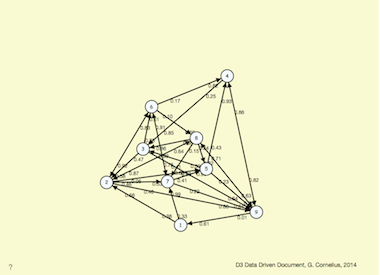
\includegraphics{randomvaluation_d3_main.png}

\end{description}

\item {} \begin{description}
\item[{Inspect function:}] \leavevmode
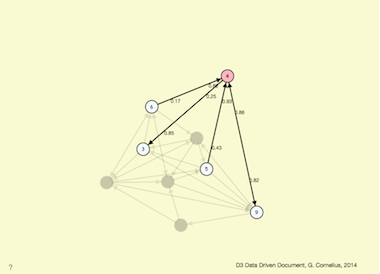
\includegraphics{randomvaluation_d3_inspect.png}

\end{description}

\end{itemize}

\end{description}

\end{enumerate}

\end{description}

\begin{notice}{note}{Note:}
If you want to use the automatic load in Chrome, try using the command: ``python -m SimpleHTTPServer'' and then access the index.html via ``\href{http://0.0.0.0:8000/index.html}{http://0.0.0.0:8000/index.html}''.
In order to load the CSS an active internet connection is needed!
\end{notice}

\end{fulllineitems}

\index{exportGraphViz() (digraphs.Digraph method)}

\begin{fulllineitems}
\phantomsection\label{techDoc:digraphs.Digraph.exportGraphViz}\pysiglinewithargsret{\bfcode{exportGraphViz}}{\emph{fileName=None}, \emph{bestChoice=set()}, \emph{worstChoice=set()}, \emph{noSilent=True}, \emph{graphType='png'}, \emph{graphSize=`7}, \emph{7'}}{}
export GraphViz dot file  for graph drawing filtering.

\end{fulllineitems}

\index{exportPrincipalImage() (digraphs.Digraph method)}

\begin{fulllineitems}
\phantomsection\label{techDoc:digraphs.Digraph.exportPrincipalImage}\pysiglinewithargsret{\bfcode{exportPrincipalImage}}{\emph{Reduced=False}, \emph{Colwise=False}, \emph{plotFileName=None}, \emph{Type='png'}, \emph{Comments=False}}{}
Export as PNG (default) or PDF the principal projection of
the valued relation using the three principal eigen vectors.

\begin{notice}{warning}{Warning:}
The method, writing and reading temporary files: 
tempCol.r and rotationCol.csv, resp. tempRow.r and rotationRow.csv,
is hence not safe for multiprocessors' threading programs.
\end{notice}

\end{fulllineitems}

\index{flatChoice() (digraphs.Digraph method)}

\begin{fulllineitems}
\phantomsection\label{techDoc:digraphs.Digraph.flatChoice}\pysiglinewithargsret{\bfcode{flatChoice}}{\emph{ch}, \emph{Debug=False}}{}
Converts set or list ch recursively to a flat list of items.

\end{fulllineitems}

\index{forcedBestSingleChoice() (digraphs.Digraph method)}

\begin{fulllineitems}
\phantomsection\label{techDoc:digraphs.Digraph.forcedBestSingleChoice}\pysiglinewithargsret{\bfcode{forcedBestSingleChoice}}{}{}
Renders the set of most determined outranking singletons in self.

\end{fulllineitems}

\index{gammaSets() (digraphs.Digraph method)}

\begin{fulllineitems}
\phantomsection\label{techDoc:digraphs.Digraph.gammaSets}\pysiglinewithargsret{\bfcode{gammaSets}}{}{}
Renders the dictionary of neighborhoods \{node: (dx,ax)\}

\end{fulllineitems}

\index{generateAbsPreKernels() (digraphs.Digraph method)}

\begin{fulllineitems}
\phantomsection\label{techDoc:digraphs.Digraph.generateAbsPreKernels}\pysiglinewithargsret{\bfcode{generateAbsPreKernels}}{}{}
Generate all absorbent prekernels from independent choices generator.

\end{fulllineitems}

\index{generateDomPreKernels() (digraphs.Digraph method)}

\begin{fulllineitems}
\phantomsection\label{techDoc:digraphs.Digraph.generateDomPreKernels}\pysiglinewithargsret{\bfcode{generateDomPreKernels}}{}{}
Generate all dominant prekernels from independent choices generator.

\end{fulllineitems}

\index{graphDetermination() (digraphs.Digraph method)}

\begin{fulllineitems}
\phantomsection\label{techDoc:digraphs.Digraph.graphDetermination}\pysiglinewithargsret{\bfcode{graphDetermination}}{}{}
Output: average arc determination

\end{fulllineitems}

\index{htmlRelationTable() (digraphs.Digraph method)}

\begin{fulllineitems}
\phantomsection\label{techDoc:digraphs.Digraph.htmlRelationTable}\pysiglinewithargsret{\bfcode{htmlRelationTable}}{\emph{tableTitle='Relation Table'}, \emph{relationName=' R `}, \emph{hasIntegerValues=False}, \emph{actionsSubset=None}, \emph{isColored=False}}{}
renders the relation valuation in actions X actions html table format.

\end{fulllineitems}

\index{inDegrees() (digraphs.Digraph method)}

\begin{fulllineitems}
\phantomsection\label{techDoc:digraphs.Digraph.inDegrees}\pysiglinewithargsret{\bfcode{inDegrees}}{}{}
renders the median cut indegrees

\end{fulllineitems}

\index{inDegreesDistribution() (digraphs.Digraph method)}

\begin{fulllineitems}
\phantomsection\label{techDoc:digraphs.Digraph.inDegreesDistribution}\pysiglinewithargsret{\bfcode{inDegreesDistribution}}{}{}
Renders the distribution of indegrees.

\end{fulllineitems}

\index{independentChoices() (digraphs.Digraph method)}

\begin{fulllineitems}
\phantomsection\label{techDoc:digraphs.Digraph.independentChoices}\pysiglinewithargsret{\bfcode{independentChoices}}{\emph{U}}{}
Generator for all independent choices with neighborhoods of a bipolar valued digraph:

\begin{notice}{note}{Note:}\begin{itemize}
\item {} 
Initiate with U = self.singletons().

\item {} 
Yields {[}(independent choice, domnb, absnb, indnb){]}.

\end{itemize}
\end{notice}

\end{fulllineitems}

\index{inner\_prod() (digraphs.Digraph method)}

\begin{fulllineitems}
\phantomsection\label{techDoc:digraphs.Digraph.inner_prod}\pysiglinewithargsret{\bfcode{inner\_prod}}{\emph{v1}, \emph{v2}}{}
Parameters: two choice characteristic vectors
Renders the inner product of two characteristic vetors.

\end{fulllineitems}

\index{intstab() (digraphs.Digraph method)}

\begin{fulllineitems}
\phantomsection\label{techDoc:digraphs.Digraph.intstab}\pysiglinewithargsret{\bfcode{intstab}}{\emph{choice}}{}
Computes the independence degree of a choice.

\end{fulllineitems}

\index{irreflex() (digraphs.Digraph method)}

\begin{fulllineitems}
\phantomsection\label{techDoc:digraphs.Digraph.irreflex}\pysiglinewithargsret{\bfcode{irreflex}}{\emph{mat}}{}
puts diagonal entries of mat to valuationdomain{[}'min'{]}

\end{fulllineitems}

\index{isComplete() (digraphs.Digraph method)}

\begin{fulllineitems}
\phantomsection\label{techDoc:digraphs.Digraph.isComplete}\pysiglinewithargsret{\bfcode{isComplete}}{\emph{Debug=False}}{}
checks the completeness property of self.relation by checking
for the absence of a link between two actions!!

\begin{notice}{warning}{Warning:}
The reflexive links are ignored !!
\end{notice}

\end{fulllineitems}

\index{isCyclic() (digraphs.Digraph method)}

\begin{fulllineitems}
\phantomsection\label{techDoc:digraphs.Digraph.isCyclic}\pysiglinewithargsret{\bfcode{isCyclic}}{\emph{Debug=False}}{}
checks the cyclicity of self.relation by checking
for a reflexive loop in its transitive closure
!! self.relation is supposed to be irreflexive !!

\end{fulllineitems}

\index{isWeaklyComplete() (digraphs.Digraph method)}

\begin{fulllineitems}
\phantomsection\label{techDoc:digraphs.Digraph.isWeaklyComplete}\pysiglinewithargsret{\bfcode{isWeaklyComplete}}{\emph{Debug=False}}{}
checks the weakly completeness property of self.relation by checking
for the absence of a link between two actions!!

\begin{notice}{warning}{Warning:}
The reflexive links are ignored !!
\end{notice}

\end{fulllineitems}

\index{iterateRankingByChoosing() (digraphs.Digraph method)}

\begin{fulllineitems}
\phantomsection\label{techDoc:digraphs.Digraph.iterateRankingByChoosing}\pysiglinewithargsret{\bfcode{iterateRankingByChoosing}}{\emph{Odd=False}, \emph{CoDual=False}, \emph{Comments=True}, \emph{Debug=False}, \emph{Limited=None}}{}
Renders a ranking by choosing result when progressively eliminating
all chordless (odd only) circuits with rising valuation cut levels.
\begin{description}
\item[{Parameters}] \leavevmode
CoDual = False (default)/True
Limited = proportion (in {[}0,1{]}) * (max - med) valuationdomain

\end{description}

\end{fulllineitems}

\index{kChoices() (digraphs.Digraph method)}

\begin{fulllineitems}
\phantomsection\label{techDoc:digraphs.Digraph.kChoices}\pysiglinewithargsret{\bfcode{kChoices}}{\emph{A}, \emph{k}}{}
Renders all choices of length k from set A

\end{fulllineitems}

\index{matmult2() (digraphs.Digraph method)}

\begin{fulllineitems}
\phantomsection\label{techDoc:digraphs.Digraph.matmult2}\pysiglinewithargsret{\bfcode{matmult2}}{\emph{m}, \emph{v}}{}
Parameters: digraph relation and choice characteristic vector
matrix multiply vector by inner production

\end{fulllineitems}

\index{meanDegree() (digraphs.Digraph method)}

\begin{fulllineitems}
\phantomsection\label{techDoc:digraphs.Digraph.meanDegree}\pysiglinewithargsret{\bfcode{meanDegree}}{}{}
Renders the mean degree of self.
!!! self.size must be set previously !!!

\end{fulllineitems}

\index{meanLength() (digraphs.Digraph method)}

\begin{fulllineitems}
\phantomsection\label{techDoc:digraphs.Digraph.meanLength}\pysiglinewithargsret{\bfcode{meanLength}}{\emph{Oriented=False}}{}
Renders the (by default non-oriented) mean neighbourhoor depth of self.
!!! self.order must be set previously !!!

\end{fulllineitems}

\index{minimalChoices() (digraphs.Digraph method)}

\begin{fulllineitems}
\phantomsection\label{techDoc:digraphs.Digraph.minimalChoices}\pysiglinewithargsret{\bfcode{minimalChoices}}{\emph{S}}{}
Generates all dominant or absorbent choices of a bipolar
valued digraph.

\end{fulllineitems}

\index{minimalValuationLevelForCircuitsElimination() (digraphs.Digraph method)}

\begin{fulllineitems}
\phantomsection\label{techDoc:digraphs.Digraph.minimalValuationLevelForCircuitsElimination}\pysiglinewithargsret{\bfcode{minimalValuationLevelForCircuitsElimination}}{\emph{Odd=True}, \emph{Debug=False}, \emph{Comments=False}}{}
renders the minimal valuation level \textless{}lambda\textgreater{} that eliminates all
self.circuitsList stored odd chordless circuits from self.

\begin{notice}{warning}{Warning:}
The \textless{}lambda\textgreater{} level polarised may still contain newly appearing chordless odd circuits !
\end{notice}

\end{fulllineitems}

\index{neighbourhoodCollection() (digraphs.Digraph method)}

\begin{fulllineitems}
\phantomsection\label{techDoc:digraphs.Digraph.neighbourhoodCollection}\pysiglinewithargsret{\bfcode{neighbourhoodCollection}}{\emph{Oriented=False}, \emph{Potential=False}}{}
Renders the neighbourhood.

\end{fulllineitems}

\index{neighbourhoodDepthDistribution() (digraphs.Digraph method)}

\begin{fulllineitems}
\phantomsection\label{techDoc:digraphs.Digraph.neighbourhoodDepthDistribution}\pysiglinewithargsret{\bfcode{neighbourhoodDepthDistribution}}{\emph{Oriented=False}}{}
Renders the distribtion of neighbourhood depths.

\end{fulllineitems}

\index{notGammaSets() (digraphs.Digraph method)}

\begin{fulllineitems}
\phantomsection\label{techDoc:digraphs.Digraph.notGammaSets}\pysiglinewithargsret{\bfcode{notGammaSets}}{}{}
Renders the dictionary of not neighborhoods \{node: (dx,ax)\}

\end{fulllineitems}

\index{notaneighbors() (digraphs.Digraph method)}

\begin{fulllineitems}
\phantomsection\label{techDoc:digraphs.Digraph.notaneighbors}\pysiglinewithargsret{\bfcode{notaneighbors}}{\emph{node}}{}
Renders the set of absorbed not in-neighbors of a node.

\end{fulllineitems}

\index{notdneighbors() (digraphs.Digraph method)}

\begin{fulllineitems}
\phantomsection\label{techDoc:digraphs.Digraph.notdneighbors}\pysiglinewithargsret{\bfcode{notdneighbors}}{\emph{node}}{}
Renders the set of not dominated out-neighbors of a node.

\end{fulllineitems}

\index{omax() (digraphs.Digraph method)}

\begin{fulllineitems}
\phantomsection\label{techDoc:digraphs.Digraph.omax}\pysiglinewithargsret{\bfcode{omax}}{\emph{L}, \emph{Debug=False}}{}
epistemic disjunction for bipolar outranking characteristics
computation

\end{fulllineitems}

\index{omin() (digraphs.Digraph method)}

\begin{fulllineitems}
\phantomsection\label{techDoc:digraphs.Digraph.omin}\pysiglinewithargsret{\bfcode{omin}}{\emph{L}, \emph{Debug=False}}{}
epistemic conjunction for bipolar outranking characteristics
computation

\end{fulllineitems}

\index{optimalRankingByChoosing() (digraphs.Digraph method)}

\begin{fulllineitems}
\phantomsection\label{techDoc:digraphs.Digraph.optimalRankingByChoosing}\pysiglinewithargsret{\bfcode{optimalRankingByChoosing}}{\emph{Odd=True}, \emph{CoDual=False}, \emph{Comments=False}, \emph{Debug=False}, \emph{Limited=None}}{}
Renders a ranking by choosing result when progressively eliminating
all chordless (odd only by default) circuits with rising valuation cut levels.

Parameters:
\begin{itemize}
\item {} 
CoDual = False (default)/True

\item {} 
Limited = proportion (in {[}0,1{]}) * (max - med) of valuationdomain (default = None)

\end{itemize}

Returns the highest correlated rankingByChoosing with self or 
codual of self, depending on the CoDual flagg.

\end{fulllineitems}

\index{outDegrees() (digraphs.Digraph method)}

\begin{fulllineitems}
\phantomsection\label{techDoc:digraphs.Digraph.outDegrees}\pysiglinewithargsret{\bfcode{outDegrees}}{}{}
renders the median cut outdegrees

\end{fulllineitems}

\index{outDegreesDistribution() (digraphs.Digraph method)}

\begin{fulllineitems}
\phantomsection\label{techDoc:digraphs.Digraph.outDegreesDistribution}\pysiglinewithargsret{\bfcode{outDegreesDistribution}}{}{}
Renders the distribution of outdegrees.

\end{fulllineitems}

\index{plusirredundant() (digraphs.Digraph method)}

\begin{fulllineitems}
\phantomsection\label{techDoc:digraphs.Digraph.plusirredundant}\pysiglinewithargsret{\bfcode{plusirredundant}}{\emph{U}}{}
Generates all +irredundant choices of a digraph.

\end{fulllineitems}

\index{powerset() (digraphs.Digraph method)}

\begin{fulllineitems}
\phantomsection\label{techDoc:digraphs.Digraph.powerset}\pysiglinewithargsret{\bfcode{powerset}}{\emph{U}}{}
Generates all subsets of a set.

\end{fulllineitems}

\index{readPerrinMisset() (digraphs.Digraph method)}

\begin{fulllineitems}
\phantomsection\label{techDoc:digraphs.Digraph.readPerrinMisset}\pysiglinewithargsret{\bfcode{readPerrinMisset}}{\emph{file}}{}
read method for 0-1-char-coded MISs from perrinMIS.c curd.dat file.

\end{fulllineitems}

\index{readPerrinMissetOpt() (digraphs.Digraph method)}

\begin{fulllineitems}
\phantomsection\label{techDoc:digraphs.Digraph.readPerrinMissetOpt}\pysiglinewithargsret{\bfcode{readPerrinMissetOpt}}{\emph{file}}{}
read method for 0-1-char-coded MISs from perrinMIS.c curd.dat file.

\end{fulllineitems}

\index{readabsvector() (digraphs.Digraph method)}

\begin{fulllineitems}
\phantomsection\label{techDoc:digraphs.Digraph.readabsvector}\pysiglinewithargsret{\bfcode{readabsvector}}{\emph{x}, \emph{relation}}{}
Parameter: action x
absorbent in vector.

\end{fulllineitems}

\index{readdomvector() (digraphs.Digraph method)}

\begin{fulllineitems}
\phantomsection\label{techDoc:digraphs.Digraph.readdomvector}\pysiglinewithargsret{\bfcode{readdomvector}}{\emph{x}, \emph{relation}}{}
Parameter: action x
dominant out vector.

\end{fulllineitems}

\index{recodeValuation() (digraphs.Digraph method)}

\begin{fulllineitems}
\phantomsection\label{techDoc:digraphs.Digraph.recodeValuation}\pysiglinewithargsret{\bfcode{recodeValuation}}{\emph{newMin=-1.0}, \emph{newMax=1.0}, \emph{Debug=False}}{}
Recodes the characteristic valuation domain according
to the parameters given.

\begin{notice}{note}{Note:}
Default values gives a normalized valuation domain
\end{notice}

\end{fulllineitems}

\index{save() (digraphs.Digraph method)}

\begin{fulllineitems}
\phantomsection\label{techDoc:digraphs.Digraph.save}\pysiglinewithargsret{\bfcode{save}}{\emph{fileName='tempdigraph'}, \emph{option=None}, \emph{DecimalValuation=True}}{}
Persistent storage of a Digraph class instance in the form of
a python source code file

\end{fulllineitems}

\index{saveCSV() (digraphs.Digraph method)}

\begin{fulllineitems}
\phantomsection\label{techDoc:digraphs.Digraph.saveCSV}\pysiglinewithargsret{\bfcode{saveCSV}}{\emph{fileName='tempdigraph'}, \emph{Normalized=True}, \emph{Dual=True}, \emph{Converse=False}, \emph{Diagonal=False}, \emph{Debug=False}}{}
Persistent storage of a Digraph class instance in the form of
a csv file.

\end{fulllineitems}

\index{saveXMCDA() (digraphs.Digraph method)}

\begin{fulllineitems}
\phantomsection\label{techDoc:digraphs.Digraph.saveXMCDA}\pysiglinewithargsret{\bfcode{saveXMCDA}}{\emph{fileName='temp'}, \emph{relationName='R'}, \emph{category='random'}, \emph{subcategory='valued'}, \emph{author='digraphs Module (RB)'}, \emph{reference='saved from Python'}, \emph{valuationType='standard'}, \emph{servingD3=False}}{}
save digraph in XMCDA format.

\end{fulllineitems}

\index{saveXMCDA2() (digraphs.Digraph method)}

\begin{fulllineitems}
\phantomsection\label{techDoc:digraphs.Digraph.saveXMCDA2}\pysiglinewithargsret{\bfcode{saveXMCDA2}}{\emph{fileName='temp'}, \emph{fileExt='xmcda2'}, \emph{Comments=True}, \emph{relationName='R'}, \emph{relationType='binary'}, \emph{category='random'}, \emph{subcategory='valued'}, \emph{author='digraphs Module (RB)'}, \emph{reference='saved from Python'}, \emph{valuationType='standard'}, \emph{digits=2}, \emph{servingD3=False}}{}
save digraph in XMCDA format.

\end{fulllineitems}

\index{saveXML() (digraphs.Digraph method)}

\begin{fulllineitems}
\phantomsection\label{techDoc:digraphs.Digraph.saveXML}\pysiglinewithargsret{\bfcode{saveXML}}{\emph{name='temp'}, \emph{category='general'}, \emph{subcategory='general'}, \emph{author='digraphs Module (RB)'}, \emph{reference='saved from Python'}}{}
save digraph in XML format.

\end{fulllineitems}

\index{savedre() (digraphs.Digraph method)}

\begin{fulllineitems}
\phantomsection\label{techDoc:digraphs.Digraph.savedre}\pysiglinewithargsret{\bfcode{savedre}}{\emph{name='temp'}}{}
save digraph in nauty format.

\end{fulllineitems}

\index{sharp() (digraphs.Digraph method)}

\begin{fulllineitems}
\phantomsection\label{techDoc:digraphs.Digraph.sharp}\pysiglinewithargsret{\bfcode{sharp}}{\emph{x}, \emph{y}}{}
Paramaters: choice characteristic values.
Renders the sharpest of two characteristic values x and y.

\end{fulllineitems}

\index{sharpvec() (digraphs.Digraph method)}

\begin{fulllineitems}
\phantomsection\label{techDoc:digraphs.Digraph.sharpvec}\pysiglinewithargsret{\bfcode{sharpvec}}{\emph{v}, \emph{w}}{}
Paramaters: choice characteristic vectors.
Renders the sharpest of two characteristic vectors v and w.

\end{fulllineitems}

\index{showActions() (digraphs.Digraph method)}

\begin{fulllineitems}
\phantomsection\label{techDoc:digraphs.Digraph.showActions}\pysiglinewithargsret{\bfcode{showActions}}{}{}
presentation methods for digraphs actions

\end{fulllineitems}

\index{showAll() (digraphs.Digraph method)}

\begin{fulllineitems}
\phantomsection\label{techDoc:digraphs.Digraph.showAll}\pysiglinewithargsret{\bfcode{showAll}}{}{}
\end{fulllineitems}

\index{showAutomorphismGenerators() (digraphs.Digraph method)}

\begin{fulllineitems}
\phantomsection\label{techDoc:digraphs.Digraph.showAutomorphismGenerators}\pysiglinewithargsret{\bfcode{showAutomorphismGenerators}}{}{}
Renders the generators of the automorphism group.

\end{fulllineitems}

\index{showBadChoices() (digraphs.Digraph method)}

\begin{fulllineitems}
\phantomsection\label{techDoc:digraphs.Digraph.showBadChoices}\pysiglinewithargsret{\bfcode{showBadChoices}}{\emph{Recompute=True}}{}
Characteristic values for potentially bad choices.

\end{fulllineitems}

\index{showChoiceVector() (digraphs.Digraph method)}

\begin{fulllineitems}
\phantomsection\label{techDoc:digraphs.Digraph.showChoiceVector}\pysiglinewithargsret{\bfcode{showChoiceVector}}{\emph{ch}}{}
show procedure for annotated bipolar choices

\end{fulllineitems}

\index{showChordlessCircuits() (digraphs.Digraph method)}

\begin{fulllineitems}
\phantomsection\label{techDoc:digraphs.Digraph.showChordlessCircuits}\pysiglinewithargsret{\bfcode{showChordlessCircuits}}{}{}
show methods for (chordless) circuits in a Digraph.
Dummy for showCircuits().

\end{fulllineitems}

\index{showCircuits() (digraphs.Digraph method)}

\begin{fulllineitems}
\phantomsection\label{techDoc:digraphs.Digraph.showCircuits}\pysiglinewithargsret{\bfcode{showCircuits}}{}{}
show methods for circuits observed in a Digraph instance.

\end{fulllineitems}

\index{showComponents() (digraphs.Digraph method)}

\begin{fulllineitems}
\phantomsection\label{techDoc:digraphs.Digraph.showComponents}\pysiglinewithargsret{\bfcode{showComponents}}{}{}
\end{fulllineitems}

\index{showGoodChoices() (digraphs.Digraph method)}

\begin{fulllineitems}
\phantomsection\label{techDoc:digraphs.Digraph.showGoodChoices}\pysiglinewithargsret{\bfcode{showGoodChoices}}{\emph{Recompute=True}}{}
Characteristic values for potentially good choices.

\end{fulllineitems}

\index{showHTMLRelationTable() (digraphs.Digraph method)}

\begin{fulllineitems}
\phantomsection\label{techDoc:digraphs.Digraph.showHTMLRelationTable}\pysiglinewithargsret{\bfcode{showHTMLRelationTable}}{}{}
Launches a browser window with the colored relation table of self.

\end{fulllineitems}

\index{showInteractiveGraph() (digraphs.Digraph method)}

\begin{fulllineitems}
\phantomsection\label{techDoc:digraphs.Digraph.showInteractiveGraph}\pysiglinewithargsret{\bfcode{showInteractiveGraph}}{}{}
Save the graph and all needed files for the visualization of an interactive graph generated by the exportD3() function.
For best experience make sure to use Firefox, because other browser restrict the loading of local files.

\end{fulllineitems}

\index{showMIS() (digraphs.Digraph method)}

\begin{fulllineitems}
\phantomsection\label{techDoc:digraphs.Digraph.showMIS}\pysiglinewithargsret{\bfcode{showMIS}}{\emph{withListing=True}}{}~\begin{description}
\item[{Prints all maximal independent choices:}] \leavevmode
Result in self.misset.

\end{description}

\end{fulllineitems}

\index{showMIS\_AH() (digraphs.Digraph method)}

\begin{fulllineitems}
\phantomsection\label{techDoc:digraphs.Digraph.showMIS_AH}\pysiglinewithargsret{\bfcode{showMIS\_AH}}{\emph{withListing=True}}{}
Prints all MIS using the Hertz method.
Result saved in self.hertzmisset.

\end{fulllineitems}

\index{showMIS\_HB2() (digraphs.Digraph method)}

\begin{fulllineitems}
\phantomsection\label{techDoc:digraphs.Digraph.showMIS_HB2}\pysiglinewithargsret{\bfcode{showMIS\_HB2}}{\emph{withListing=True}}{}
Prints all MIS using the Hertz-Bisdorff method.
Result saved in self.newmisset.

\end{fulllineitems}

\index{showMIS\_RB() (digraphs.Digraph method)}

\begin{fulllineitems}
\phantomsection\label{techDoc:digraphs.Digraph.showMIS_RB}\pysiglinewithargsret{\bfcode{showMIS\_RB}}{\emph{withListing=True}}{}
Prints all MIS using the Bisdorff method.
Result saved in self.newmisset.

\end{fulllineitems}

\index{showMIS\_UD() (digraphs.Digraph method)}

\begin{fulllineitems}
\phantomsection\label{techDoc:digraphs.Digraph.showMIS_UD}\pysiglinewithargsret{\bfcode{showMIS\_UD}}{\emph{withListing=True}}{}
Prints all MIS using the Hertz-Bisdorff method.
Result saved in self.newmisset.

\end{fulllineitems}

\index{showMaxAbsIrred() (digraphs.Digraph method)}

\begin{fulllineitems}
\phantomsection\label{techDoc:digraphs.Digraph.showMaxAbsIrred}\pysiglinewithargsret{\bfcode{showMaxAbsIrred}}{\emph{withListing=True}}{}~\begin{description}
\item[{Computing maximal -irredundant choices:}] \leavevmode
Result in self.absirset.

\end{description}

\end{fulllineitems}

\index{showMaxDomIrred() (digraphs.Digraph method)}

\begin{fulllineitems}
\phantomsection\label{techDoc:digraphs.Digraph.showMaxDomIrred}\pysiglinewithargsret{\bfcode{showMaxDomIrred}}{\emph{withListing=True}}{}~\begin{description}
\item[{Computing maximal +irredundant choices:}] \leavevmode
Result in self.domirset.

\end{description}

\end{fulllineitems}

\index{showMinAbs() (digraphs.Digraph method)}

\begin{fulllineitems}
\phantomsection\label{techDoc:digraphs.Digraph.showMinAbs}\pysiglinewithargsret{\bfcode{showMinAbs}}{\emph{withListing=True}}{}~\begin{description}
\item[{Prints minimal absorbent choices:}] \leavevmode
Result in self.absset.

\end{description}

\end{fulllineitems}

\index{showMinDom() (digraphs.Digraph method)}

\begin{fulllineitems}
\phantomsection\label{techDoc:digraphs.Digraph.showMinDom}\pysiglinewithargsret{\bfcode{showMinDom}}{\emph{withListing=True}}{}~\begin{description}
\item[{Prints all minimal dominant choices:}] \leavevmode
Result in self.domset.

\end{description}

\end{fulllineitems}

\index{showNeighborhoods() (digraphs.Digraph method)}

\begin{fulllineitems}
\phantomsection\label{techDoc:digraphs.Digraph.showNeighborhoods}\pysiglinewithargsret{\bfcode{showNeighborhoods}}{}{}
Lists the gamma and the notGamma function of self.

\end{fulllineitems}

\index{showOrbits() (digraphs.Digraph method)}

\begin{fulllineitems}
\phantomsection\label{techDoc:digraphs.Digraph.showOrbits}\pysiglinewithargsret{\bfcode{showOrbits}}{\emph{InChoices}, \emph{withListing=True}}{}
Prints the orbits of Choices along the automorphisms of
the digraph self.

\end{fulllineitems}

\index{showOrbitsFromFile() (digraphs.Digraph method)}

\begin{fulllineitems}
\phantomsection\label{techDoc:digraphs.Digraph.showOrbitsFromFile}\pysiglinewithargsret{\bfcode{showOrbitsFromFile}}{\emph{InFile}, \emph{withListing=True}}{}
Prints the orbits of Choices along the automorphisms of
the digraph self by reading in the 0-1 misset file format.

\end{fulllineitems}

\index{showPreKernels() (digraphs.Digraph method)}

\begin{fulllineitems}
\phantomsection\label{techDoc:digraphs.Digraph.showPreKernels}\pysiglinewithargsret{\bfcode{showPreKernels}}{\emph{withListing=True}}{}~\begin{description}
\item[{Printing dominant and absorbent preKernels:}] \leavevmode
Result in self.dompreKernels and self.abspreKernels

\end{description}

\end{fulllineitems}

\index{showRankingByBestChoosing() (digraphs.Digraph method)}

\begin{fulllineitems}
\phantomsection\label{techDoc:digraphs.Digraph.showRankingByBestChoosing}\pysiglinewithargsret{\bfcode{showRankingByBestChoosing}}{\emph{rankingByBestChoosing=None}}{}
A show method for self.rankinByBestChoosing result.

\begin{notice}{warning}{Warning:}
The self.computeRankingByBestChoosing(CoDual=False/True) method instantiating the self.rankingByBestChoosing slot is pre-required !
\end{notice}

\end{fulllineitems}

\index{showRankingByChoosing() (digraphs.Digraph method)}

\begin{fulllineitems}
\phantomsection\label{techDoc:digraphs.Digraph.showRankingByChoosing}\pysiglinewithargsret{\bfcode{showRankingByChoosing}}{\emph{rankingByChoosing=None}}{}
A show method for self.rankinByChoosing result.

\begin{notice}{warning}{Warning:}
The self.computeRankingByChoosing(CoDual=False/True) method instantiating the self.rankingByChoosing slot is pre-required !
\end{notice}

\end{fulllineitems}

\index{showRankingByLastChoosing() (digraphs.Digraph method)}

\begin{fulllineitems}
\phantomsection\label{techDoc:digraphs.Digraph.showRankingByLastChoosing}\pysiglinewithargsret{\bfcode{showRankingByLastChoosing}}{\emph{rankingByLastChoosing=None}, \emph{Debug=None}}{}
A show method for self.rankinByChoosing result.

\begin{notice}{warning}{Warning:}
The self.computeRankingByLastChoosing(CoDual=False/True) method instantiating the self.rankingByChoosing slot is pre-required !
\end{notice}

\end{fulllineitems}

\index{showRelation() (digraphs.Digraph method)}

\begin{fulllineitems}
\phantomsection\label{techDoc:digraphs.Digraph.showRelation}\pysiglinewithargsret{\bfcode{showRelation}}{}{}
prints the relation valuation in \#\#.\#\# format.

\end{fulllineitems}

\index{showRelationTable() (digraphs.Digraph method)}

\begin{fulllineitems}
\phantomsection\label{techDoc:digraphs.Digraph.showRelationTable}\pysiglinewithargsret{\bfcode{showRelationTable}}{\emph{Sorted=True}, \emph{IntegerValues=False}, \emph{actionsSubset=None}, \emph{relation=None}, \emph{ndigits=2}, \emph{ReflexiveTerms=True}}{}
prints the relation valuation in actions X actions table format.

\end{fulllineitems}

\index{showRubisBestChoiceRecommendation() (digraphs.Digraph method)}

\begin{fulllineitems}
\phantomsection\label{techDoc:digraphs.Digraph.showRubisBestChoiceRecommendation}\pysiglinewithargsret{\bfcode{showRubisBestChoiceRecommendation}}{\emph{Comments=False}, \emph{Debug=False}}{}
Renders the RuBis best choice recommendation.

\end{fulllineitems}

\index{showRubyChoice() (digraphs.Digraph method)}

\begin{fulllineitems}
\phantomsection\label{techDoc:digraphs.Digraph.showRubyChoice}\pysiglinewithargsret{\bfcode{showRubyChoice}}{\emph{Comments=False}}{}
dummy for showRubisChoice()
older versions compatibility

\end{fulllineitems}

\index{showShort() (digraphs.Digraph method)}

\begin{fulllineitems}
\phantomsection\label{techDoc:digraphs.Digraph.showShort}\pysiglinewithargsret{\bfcode{showShort}}{}{}
concise presentation method for genuine digraphs.

\end{fulllineitems}

\index{showSingletonRanking() (digraphs.Digraph method)}

\begin{fulllineitems}
\phantomsection\label{techDoc:digraphs.Digraph.showSingletonRanking}\pysiglinewithargsret{\bfcode{showSingletonRanking}}{\emph{Comments=True}, \emph{Debug=False}}{}
Calls self.computeSingletonRanking(comments=True,Debug = False).
Renders and prints the sorted bipolar net determinatation of outrankingness
minus outrankedness credibilities of all singleton choices.
res = ((netdet,sigleton,dom,absorb)+)

\end{fulllineitems}

\index{showStatistics() (digraphs.Digraph method)}

\begin{fulllineitems}
\phantomsection\label{techDoc:digraphs.Digraph.showStatistics}\pysiglinewithargsret{\bfcode{showStatistics}}{}{}
Computes digraph statistics like order, size and arc-density.

\end{fulllineitems}

\index{showdre() (digraphs.Digraph method)}

\begin{fulllineitems}
\phantomsection\label{techDoc:digraphs.Digraph.showdre}\pysiglinewithargsret{\bfcode{showdre}}{}{}
Shows relation in nauty format.

\end{fulllineitems}

\index{singletons() (digraphs.Digraph method)}

\begin{fulllineitems}
\phantomsection\label{techDoc:digraphs.Digraph.singletons}\pysiglinewithargsret{\bfcode{singletons}}{}{}
list of singletons and neighborhoods
{[}(singx1, +nx1, -nx1, not(+nx1 or -nx1)),.... {]}

\end{fulllineitems}

\index{size() (digraphs.Digraph method)}

\begin{fulllineitems}
\phantomsection\label{techDoc:digraphs.Digraph.size}\pysiglinewithargsret{\bfcode{size}}{}{}
Renders the number of validated non reflexive arcs

\end{fulllineitems}

\index{sizeSubGraph() (digraphs.Digraph method)}

\begin{fulllineitems}
\phantomsection\label{techDoc:digraphs.Digraph.sizeSubGraph}\pysiglinewithargsret{\bfcode{sizeSubGraph}}{\emph{choice}}{}
Output: (size, undeterm,arcDensity).
Renders the arc density of the induced subgraph.

\end{fulllineitems}

\index{strongComponents() (digraphs.Digraph method)}

\begin{fulllineitems}
\phantomsection\label{techDoc:digraphs.Digraph.strongComponents}\pysiglinewithargsret{\bfcode{strongComponents}}{\emph{setPotential=False}}{}
Renders the set of strong components of self.

\end{fulllineitems}

\index{symDegreesDistribution() (digraphs.Digraph method)}

\begin{fulllineitems}
\phantomsection\label{techDoc:digraphs.Digraph.symDegreesDistribution}\pysiglinewithargsret{\bfcode{symDegreesDistribution}}{}{}
Renders the distribution of symmetric degrees.

\end{fulllineitems}

\index{topologicalSort() (digraphs.Digraph method)}

\begin{fulllineitems}
\phantomsection\label{techDoc:digraphs.Digraph.topologicalSort}\pysiglinewithargsret{\bfcode{topologicalSort}}{\emph{Debug=False}}{}
If self is acyclic, adds topological sort number to each node of self
and renders ordered list of nodes. Otherwise renders None.
Source: M. Golumbic Algorithmic Graph heory and Perfect Graphs,
Annals Of Discrete Mathematics 57 2nd Ed. , Elsevier 2004, Algorithm 2.4 p.44.

\end{fulllineitems}

\index{weakAneighbors() (digraphs.Digraph method)}

\begin{fulllineitems}
\phantomsection\label{techDoc:digraphs.Digraph.weakAneighbors}\pysiglinewithargsret{\bfcode{weakAneighbors}}{\emph{node}}{}
Renders the set of absorbed in-neighbors of a node.

\end{fulllineitems}

\index{weakCondorcetWinners() (digraphs.Digraph method)}

\begin{fulllineitems}
\phantomsection\label{techDoc:digraphs.Digraph.weakCondorcetWinners}\pysiglinewithargsret{\bfcode{weakCondorcetWinners}}{}{}
Renders the set of decision actions x such that
self.relation{[}x{]}{[}y{]} \textgreater{}= self.valuationdomain{[}'med'{]}
for all y != x.

\end{fulllineitems}

\index{weakDneighbors() (digraphs.Digraph method)}

\begin{fulllineitems}
\phantomsection\label{techDoc:digraphs.Digraph.weakDneighbors}\pysiglinewithargsret{\bfcode{weakDneighbors}}{\emph{node}}{}
Renders the set of dominated out-neighbors of a node.

\end{fulllineitems}

\index{weakGammaSets() (digraphs.Digraph method)}

\begin{fulllineitems}
\phantomsection\label{techDoc:digraphs.Digraph.weakGammaSets}\pysiglinewithargsret{\bfcode{weakGammaSets}}{}{}
Renders the dictionary of neighborhoods \{node: (dx,ax)\}

\end{fulllineitems}

\index{worstRanks() (digraphs.Digraph method)}

\begin{fulllineitems}
\phantomsection\label{techDoc:digraphs.Digraph.worstRanks}\pysiglinewithargsret{\bfcode{worstRanks}}{}{}
renders worst possible ranks from outdegrees account

\end{fulllineitems}

\index{zoomValuation() (digraphs.Digraph method)}

\begin{fulllineitems}
\phantomsection\label{techDoc:digraphs.Digraph.zoomValuation}\pysiglinewithargsret{\bfcode{zoomValuation}}{\emph{zoomFactor=1.0}}{}
Zooms in or out, depending on the value of the zoomFactor provided,
the bipolar valuation of a digraph.

\end{fulllineitems}


\end{fulllineitems}

\index{DualDigraph (class in digraphs)}

\begin{fulllineitems}
\phantomsection\label{techDoc:digraphs.DualDigraph}\pysiglinewithargsret{\strong{class }\code{digraphs.}\bfcode{DualDigraph}}{\emph{other}}{}
Bases: {\hyperref[techDoc:digraphs.Digraph]{\code{digraphs.Digraph}}}

Instantiates the dual Digraph object of a given other Digraph instance.
\begin{description}
\item[{The relation constructor returns the dual of self.relation with formula:}] \leavevmode
relationOut{[}a{]}{[}b{]} = Max - self.relation{[}a{]}{[}b{]} + Min
where Max (resp. Min) equals valuation maximum (resp. minimum).

\end{description}

\end{fulllineitems}

\index{EmptyDigraph (class in digraphs)}

\begin{fulllineitems}
\phantomsection\label{techDoc:digraphs.EmptyDigraph}\pysiglinewithargsret{\strong{class }\code{digraphs.}\bfcode{EmptyDigraph}}{\emph{order=5}, \emph{valuationdomain=(-1.0}, \emph{1.0)}}{}
Bases: {\hyperref[techDoc:digraphs.Digraph]{\code{digraphs.Digraph}}}
\begin{description}
\item[{Parameters:}] \leavevmode
order \textgreater{} 0 (default=5); valuationdomain =(Min,Max).

\end{description}

Specialization of the general Digraph class for generating
temporary empty graphs of given order in \{-1,0,1\}.

\end{fulllineitems}

\index{EquivalenceDigraph (class in digraphs)}

\begin{fulllineitems}
\phantomsection\label{techDoc:digraphs.EquivalenceDigraph}\pysiglinewithargsret{\strong{class }\code{digraphs.}\bfcode{EquivalenceDigraph}}{\emph{d1}, \emph{d2}, \emph{Debug=False}}{}
Bases: {\hyperref[techDoc:digraphs.Digraph]{\code{digraphs.Digraph}}}

Instantiates the logical equivalence digraph of two bipolar
digraphs d1 and d2 of same order. Returns None if d1 and d2 are of different order
\index{computeCorrelation() (digraphs.EquivalenceDigraph method)}

\begin{fulllineitems}
\phantomsection\label{techDoc:digraphs.EquivalenceDigraph.computeCorrelation}\pysiglinewithargsret{\bfcode{computeCorrelation}}{}{}
Renders the global bipolar correlation index resulting from the pairwise
equivalence valuations.

\end{fulllineitems}


\end{fulllineitems}

\index{FusionDigraph (class in digraphs)}

\begin{fulllineitems}
\phantomsection\label{techDoc:digraphs.FusionDigraph}\pysiglinewithargsret{\strong{class }\code{digraphs.}\bfcode{FusionDigraph}}{\emph{dg1}, \emph{dg2}, \emph{operator='o-min'}}{}
Bases: {\hyperref[techDoc:digraphs.Digraph]{\code{digraphs.Digraph}}}

Instantiates the epistemic fusion of two given Digraph called dg1 and dg2.

Parameter:
\begin{itemize}
\item {} 
operator = ``o-min'' \textbar{} ``o-max'' (epistemic conjunctive or dijunctive fusion)

\end{itemize}

\end{fulllineitems}

\index{GridDigraph (class in digraphs)}

\begin{fulllineitems}
\phantomsection\label{techDoc:digraphs.GridDigraph}\pysiglinewithargsret{\strong{class }\code{digraphs.}\bfcode{GridDigraph}}{\emph{n=5}, \emph{m=5}, \emph{valuationdomain=\{`max': 1.0}, \emph{`min': -1.0\}}, \emph{hasRandomOrientation=False}, \emph{hasMedianSplitOrientation=False}}{}
Bases: {\hyperref[techDoc:digraphs.Digraph]{\code{digraphs.Digraph}}}
\begin{description}
\item[{Parameters:}] \leavevmode
n,m \textgreater{} 0; valuationdomain =\{`min':m, `max':M\}.

\end{description}

Specialization of the general Digraph class for generating
temporary Grid digraphs of dimension n times m.
\begin{description}
\item[{Default instantiation (5 times 5 Grid Digraph):}] \leavevmode
n = 5, m=5, valuationdomain = \{`min':-1.0,'max':1.0\}.

\end{description}

Randomly orientable with hasRandomOrientation=True (default=False).
\index{showShort() (digraphs.GridDigraph method)}

\begin{fulllineitems}
\phantomsection\label{techDoc:digraphs.GridDigraph.showShort}\pysiglinewithargsret{\bfcode{showShort}}{}{}
\end{fulllineitems}


\end{fulllineitems}

\index{IndeterminateDigraph (class in digraphs)}

\begin{fulllineitems}
\phantomsection\label{techDoc:digraphs.IndeterminateDigraph}\pysiglinewithargsret{\strong{class }\code{digraphs.}\bfcode{IndeterminateDigraph}}{\emph{other=None}, \emph{order=5}, \emph{valuationdomain=(-1.0}, \emph{1.0)}}{}
Bases: {\hyperref[techDoc:digraphs.Digraph]{\code{digraphs.Digraph}}}

Parameters: order \textgreater{} 0; valuationdomain =(Min,Max).
Specialization of the general Digraph class for generating
temporary empty graphs of order 5 in \{-1,0,1\}.

\end{fulllineitems}

\index{KneserDigraph (class in digraphs)}

\begin{fulllineitems}
\phantomsection\label{techDoc:digraphs.KneserDigraph}\pysiglinewithargsret{\strong{class }\code{digraphs.}\bfcode{KneserDigraph}}{\emph{n=5}, \emph{j=2}, \emph{valuationdomain=\{`max': 1.0}, \emph{`min': -1.0\}}}{}
Bases: {\hyperref[techDoc:digraphs.Digraph]{\code{digraphs.Digraph}}}
\begin{description}
\item[{Parameters:}] \leavevmode
\begin{DUlineblock}{0em}
\item[] n \textgreater{} 0; n \textgreater{} j \textgreater{} 0;
\item[] valuationdomain =\{`min':m, `max':M\}.
\end{DUlineblock}

\end{description}

Specialization of the general Digraph class for generating
temporary Kneser digraphs
\begin{description}
\item[{Default instantiation as Petersen graph:}] \leavevmode
n = 5, j = 2, valuationdomain = \{`min':-1.0,'max':1.0\}.

\end{description}
\index{showShort() (digraphs.KneserDigraph method)}

\begin{fulllineitems}
\phantomsection\label{techDoc:digraphs.KneserDigraph.showShort}\pysiglinewithargsret{\bfcode{showShort}}{}{}
\end{fulllineitems}


\end{fulllineitems}

\index{MedianExtendedDigraph (class in digraphs)}

\begin{fulllineitems}
\phantomsection\label{techDoc:digraphs.MedianExtendedDigraph}\pysiglinewithargsret{\strong{class }\code{digraphs.}\bfcode{MedianExtendedDigraph}}{\emph{digraph=None}, \emph{Level=None}}{}
Bases: {\hyperref[techDoc:digraphs.Digraph]{\code{digraphs.Digraph}}}
\begin{description}
\item[{Parameters:}] \leavevmode
digraph + beta cut level between Med and Max.

\end{description}

Specialisation of Outranking relation.
\index{constructRelation() (digraphs.MedianExtendedDigraph method)}

\begin{fulllineitems}
\phantomsection\label{techDoc:digraphs.MedianExtendedDigraph.constructRelation}\pysiglinewithargsret{\bfcode{constructRelation}}{\emph{relationin}, \emph{Level}}{}
Parameters: relation and cut level.
Renders the polarised relation.

\end{fulllineitems}


\end{fulllineitems}

\index{PolarisedDigraph (class in digraphs)}

\begin{fulllineitems}
\phantomsection\label{techDoc:digraphs.PolarisedDigraph}\pysiglinewithargsret{\strong{class }\code{digraphs.}\bfcode{PolarisedDigraph}}{\emph{digraph=None}, \emph{level=None}, \emph{KeepValues=True}, \emph{AlphaCut=False}, \emph{StrictCut=False}}{}
Bases: {\hyperref[techDoc:digraphs.Digraph]{\code{digraphs.Digraph}}}
\begin{description}
\item[{Renders the polarised valuation of digraph:}] \leavevmode\begin{itemize}
\item {} 
If AlphaCut = True a genuine one-sided True-oriented cut is operated.

\item {} 
If StrictCut = True, the cut level value is not included.

\end{itemize}

\end{description}

\end{fulllineitems}

\index{PreferenceDigraph (class in digraphs)}

\begin{fulllineitems}
\phantomsection\label{techDoc:digraphs.PreferenceDigraph}\pysiglinewithargsret{\strong{class }\code{digraphs.}\bfcode{PreferenceDigraph}}{\emph{digraph}}{}
Bases: {\hyperref[techDoc:digraphs.Digraph]{\code{digraphs.Digraph}}}

Initiates the valued difference S(a,b) - S(b,a) of a Digraph instance.

\end{fulllineitems}

\index{Preorder (class in digraphs)}

\begin{fulllineitems}
\phantomsection\label{techDoc:digraphs.Preorder}\pysiglinewithargsret{\strong{class }\code{digraphs.}\bfcode{Preorder}}{\emph{other}, \emph{direction='best'}}{}
Bases: {\hyperref[techDoc:digraphs.Digraph]{\code{digraphs.Digraph}}}

Instantiates the associated preorder from
a given Digraph called other.

Instantiates as other.\_\_class\_\_ !

Copies the case given the description, the criteria
and the evaluation dictionary into self.

\end{fulllineitems}

\index{RandomDigraph (class in digraphs)}

\begin{fulllineitems}
\phantomsection\label{techDoc:digraphs.RandomDigraph}\pysiglinewithargsret{\strong{class }\code{digraphs.}\bfcode{RandomDigraph}}{\emph{order=9}, \emph{arcProbability=0.5}, \emph{hasIntegerValuation=True}, \emph{Bipolar=False}}{}
Bases: {\hyperref[techDoc:digraphs.Digraph]{\code{digraphs.Digraph}}}

Specialization of the general Digraph class for generating
temporary crisp (irreflexive) random digraphs.
\begin{description}
\item[{\emph{Parameters}:}] \leavevmode\begin{itemize}
\item {} 
order (default = 10);

\item {} 
arc\_probability (in {[}0.,1.{]}, default=0.5)

\item {} 
\end{itemize}

\end{description}

\end{fulllineitems}

\index{RandomFixedDegreeSequenceDigraph (class in digraphs)}

\begin{fulllineitems}
\phantomsection\label{techDoc:digraphs.RandomFixedDegreeSequenceDigraph}\pysiglinewithargsret{\strong{class }\code{digraphs.}\bfcode{RandomFixedDegreeSequenceDigraph}}{\emph{order=7, degreeSequence={[}3, 3, 2, 2, 1, 1, 0{]}}}{}
Bases: {\hyperref[techDoc:digraphs.Digraph]{\code{digraphs.Digraph}}}
\begin{description}
\item[{Parameters:}] \leavevmode
order=n and degreeSequence={[}degree\_1, ... ,degree\_n{]}\textgreater{}

\end{description}

Specialization of Digraph class for random symmetric instances
with fixed degree sequence.

\end{fulllineitems}

\index{RandomFixedSizeDigraph (class in digraphs)}

\begin{fulllineitems}
\phantomsection\label{techDoc:digraphs.RandomFixedSizeDigraph}\pysiglinewithargsret{\strong{class }\code{digraphs.}\bfcode{RandomFixedSizeDigraph}}{\emph{order=7}, \emph{size=14}}{}
Bases: {\hyperref[techDoc:digraphs.Digraph]{\code{digraphs.Digraph}}}
\begin{description}
\item[{Parameters:}] \leavevmode
order and size

\end{description}

Specialization of Digraph class for random fixed size instances.

\end{fulllineitems}

\index{RandomRegularDigraph (class in digraphs)}

\begin{fulllineitems}
\phantomsection\label{techDoc:digraphs.RandomRegularDigraph}\pysiglinewithargsret{\strong{class }\code{digraphs.}\bfcode{RandomRegularDigraph}}{\emph{order=7}, \emph{degree=2}}{}
Bases: {\hyperref[techDoc:digraphs.Digraph]{\code{digraphs.Digraph}}}
\begin{description}
\item[{Parameters:}] \leavevmode
order and degree.

\end{description}

Specialization of Digraph class for random regular symmetric instances.

\end{fulllineitems}

\index{RandomTournament (class in digraphs)}

\begin{fulllineitems}
\phantomsection\label{techDoc:digraphs.RandomTournament}\pysiglinewithargsret{\strong{class }\code{digraphs.}\bfcode{RandomTournament}}{\emph{order=10}, \emph{ndigits=2}, \emph{isCrisp=True}, \emph{valuationDomain=None}}{}
Bases: {\hyperref[techDoc:digraphs.Digraph]{\code{digraphs.Digraph}}}
\begin{description}
\item[{Parameter:}] \leavevmode
order = n \textgreater{} 0

\end{description}

Specialization of the general Digraph class for generating
temporary weak tournaments

\end{fulllineitems}

\index{RandomTree (class in digraphs)}

\begin{fulllineitems}
\phantomsection\label{techDoc:digraphs.RandomTree}\pysiglinewithargsret{\strong{class }\code{digraphs.}\bfcode{RandomTree}}{\emph{numberOfNodes=5}, \emph{ndigits=2}, \emph{hasIntegerValuation=True}}{}
Bases: {\hyperref[techDoc:digraphs.Digraph]{\code{digraphs.Digraph}}}

Random generator for trees, using random Pruefer codes
\begin{description}
\item[{Parameter:}] \leavevmode
numerOfNodes

\end{description}
\index{prufer\_to\_tree() (digraphs.RandomTree method)}

\begin{fulllineitems}
\phantomsection\label{techDoc:digraphs.RandomTree.prufer_to_tree}\pysiglinewithargsret{\bfcode{prufer\_to\_tree}}{\emph{a}}{}
\end{fulllineitems}


\end{fulllineitems}

\index{RandomValuationDigraph (class in digraphs)}

\begin{fulllineitems}
\phantomsection\label{techDoc:digraphs.RandomValuationDigraph}\pysiglinewithargsret{\strong{class }\code{digraphs.}\bfcode{RandomValuationDigraph}}{\emph{order=9}, \emph{ndigits=2}, \emph{Normalized=False}, \emph{hasIntegerValuation=False}}{}
Bases: {\hyperref[techDoc:digraphs.Digraph]{\code{digraphs.Digraph}}}

Specialization of the general Digraph class for generating
temporary uniformly valuated random digraphs.
\begin{description}
\item[{\emph{Parameters}:}] \leavevmode\begin{itemize}
\item {} 
order \textgreater{} 0, number of arcs;

\item {} 
ndigits \textgreater{} 0, number of digits if hasIntegerValuation = True;
Otherwise, decimal precision.

\item {} 
Normalized = True (r in {[}-1,1{]}, r in {[}0,1{]} if False/default);

\item {} 
hasIntegerValuation = False (default).

\end{itemize}

\item[{Example python3 session:}] \leavevmode
\begin{Verbatim}[commandchars=\\\{\}]
\PYG{g+gp}{\PYGZgt{}\PYGZgt{}\PYGZgt{} }\PYG{k+kn}{from} \PYG{n+nn}{digraphs} \PYG{k+kn}{import} \PYG{n}{RandomValuationDigraph}
\PYG{g+gp}{\PYGZgt{}\PYGZgt{}\PYGZgt{} }\PYG{n}{dg} \PYG{o}{=} \PYG{n}{RandomValuationDigraph}\PYG{p}{(}\PYG{n}{order}\PYG{o}{=}\PYG{l+m+mi}{5}\PYG{p}{,}\PYG{n}{Normalized}\PYG{o}{=}\PYG{n+nb+bp}{True}\PYG{p}{)}
\PYG{g+gp}{\PYGZgt{}\PYGZgt{}\PYGZgt{} }\PYG{n}{dg}\PYG{o}{.}\PYG{n}{showAll}\PYG{p}{(}\PYG{p}{)}
\PYG{g+go}{*\PYGZhy{}\PYGZhy{}\PYGZhy{}\PYGZhy{}\PYGZhy{} show detail \PYGZhy{}\PYGZhy{}\PYGZhy{}\PYGZhy{}\PYGZhy{}\PYGZhy{}\PYGZhy{}\PYGZhy{}\PYGZhy{}\PYGZhy{}\PYGZhy{}\PYGZhy{}\PYGZhy{}*}
\PYG{g+go}{Digraph          : randomValuationDigraph}
\PYG{g+go}{*\PYGZhy{}\PYGZhy{}\PYGZhy{}\PYGZhy{} Actions \PYGZhy{}\PYGZhy{}\PYGZhy{}\PYGZhy{}*}
\PYG{g+go}{[\PYGZsq{}1\PYGZsq{}, \PYGZsq{}2\PYGZsq{}, \PYGZsq{}3\PYGZsq{}, \PYGZsq{}4\PYGZsq{}, \PYGZsq{}5\PYGZsq{}]}
\PYG{g+go}{*\PYGZhy{}\PYGZhy{}\PYGZhy{}\PYGZhy{} Characteristic valuation domain \PYGZhy{}\PYGZhy{}\PYGZhy{}\PYGZhy{}*}
\PYG{g+go}{\PYGZob{}\PYGZsq{}max\PYGZsq{}: Decimal(\PYGZsq{}1.0\PYGZsq{}), \PYGZsq{}min\PYGZsq{}: Decimal(\PYGZsq{}\PYGZhy{}1.0\PYGZsq{}),}
\PYG{g+go}{ \PYGZsq{}med\PYGZsq{}: Decimal(\PYGZsq{}0.0\PYGZsq{}), \PYGZsq{}hasIntegerValuation\PYGZsq{}: False\PYGZcb{}}
\PYG{g+go}{* \PYGZhy{}\PYGZhy{}\PYGZhy{}\PYGZhy{} Relation Table \PYGZhy{}\PYGZhy{}\PYGZhy{}\PYGZhy{}\PYGZhy{}}
\PYG{g+go}{  S   \textbar{}  \PYGZsq{}1\PYGZsq{}    \PYGZsq{}2\PYGZsq{}    \PYGZsq{}3\PYGZsq{}    \PYGZsq{}4\PYGZsq{}     \PYGZsq{}5\PYGZsq{}     }
\PYG{g+go}{ \PYGZhy{}\PYGZhy{}\PYGZhy{}\PYGZhy{}\PYGZhy{}\textbar{}\PYGZhy{}\PYGZhy{}\PYGZhy{}\PYGZhy{}\PYGZhy{}\PYGZhy{}\PYGZhy{}\PYGZhy{}\PYGZhy{}\PYGZhy{}\PYGZhy{}\PYGZhy{}\PYGZhy{}\PYGZhy{}\PYGZhy{}\PYGZhy{}\PYGZhy{}\PYGZhy{}\PYGZhy{}\PYGZhy{}\PYGZhy{}\PYGZhy{}\PYGZhy{}\PYGZhy{}\PYGZhy{}\PYGZhy{}\PYGZhy{}\PYGZhy{}\PYGZhy{}\PYGZhy{}\PYGZhy{}\PYGZhy{}\PYGZhy{}\PYGZhy{}\PYGZhy{}}
\PYG{g+go}{  \PYGZsq{}1\PYGZsq{} \textbar{}  0.00   0.28   0.46  \PYGZhy{}0.66   0.90    }
\PYG{g+go}{  \PYGZsq{}2\PYGZsq{} \textbar{} \PYGZhy{}0.08   0.00  \PYGZhy{}0.46  \PYGZhy{}0.42   0.52    }
\PYG{g+go}{  \PYGZsq{}3\PYGZsq{} \textbar{}  0.84  \PYGZhy{}0.10   0.00  \PYGZhy{}0.54   0.58    }
\PYG{g+go}{  \PYGZsq{}4\PYGZsq{} \textbar{}  0.90   0.88   0.90   0.00  \PYGZhy{}0.38    }
\PYG{g+go}{  \PYGZsq{}5\PYGZsq{} \textbar{} \PYGZhy{}0.50   0.64   0.42  \PYGZhy{}0.94   0.00    }
\PYG{g+go}{*\PYGZhy{}\PYGZhy{}\PYGZhy{} Connected Components \PYGZhy{}\PYGZhy{}\PYGZhy{}*}
\PYG{g+go}{1: [\PYGZsq{}1\PYGZsq{}, \PYGZsq{}2\PYGZsq{}, \PYGZsq{}3\PYGZsq{}, \PYGZsq{}4\PYGZsq{}, \PYGZsq{}5\PYGZsq{}]}
\PYG{g+go}{Neighborhoods:}
\PYG{g+go}{  Gamma     :}
\PYG{g+go}{\PYGZsq{}4\PYGZsq{}: in =\PYGZgt{} set(), out =\PYGZgt{} \PYGZob{}\PYGZsq{}1\PYGZsq{}, \PYGZsq{}2\PYGZsq{}, \PYGZsq{}3\PYGZsq{}\PYGZcb{}}
\PYG{g+go}{\PYGZsq{}5\PYGZsq{}: in =\PYGZgt{} \PYGZob{}\PYGZsq{}1\PYGZsq{}, \PYGZsq{}2\PYGZsq{}, \PYGZsq{}3\PYGZsq{}\PYGZcb{}, out =\PYGZgt{} \PYGZob{}\PYGZsq{}2\PYGZsq{}, \PYGZsq{}3\PYGZsq{}\PYGZcb{}}
\PYG{g+go}{\PYGZsq{}1\PYGZsq{}: in =\PYGZgt{} \PYGZob{}\PYGZsq{}4\PYGZsq{}, \PYGZsq{}3\PYGZsq{}\PYGZcb{}, out =\PYGZgt{} \PYGZob{}\PYGZsq{}5\PYGZsq{}, \PYGZsq{}2\PYGZsq{}, \PYGZsq{}3\PYGZsq{}\PYGZcb{}}
\PYG{g+go}{\PYGZsq{}2\PYGZsq{}: in =\PYGZgt{} \PYGZob{}\PYGZsq{}4\PYGZsq{}, \PYGZsq{}5\PYGZsq{}, \PYGZsq{}1\PYGZsq{}\PYGZcb{}, out =\PYGZgt{} \PYGZob{}\PYGZsq{}5\PYGZsq{}\PYGZcb{}}
\PYG{g+go}{\PYGZsq{}3\PYGZsq{}: in =\PYGZgt{} \PYGZob{}\PYGZsq{}4\PYGZsq{}, \PYGZsq{}5\PYGZsq{}, \PYGZsq{}1\PYGZsq{}\PYGZcb{}, out =\PYGZgt{} \PYGZob{}\PYGZsq{}5\PYGZsq{}, \PYGZsq{}1\PYGZsq{}\PYGZcb{}}
\PYG{g+go}{  Not Gamma :}
\PYG{g+go}{\PYGZsq{}4\PYGZsq{}: in =\PYGZgt{} \PYGZob{}\PYGZsq{}5\PYGZsq{}, \PYGZsq{}1\PYGZsq{}, \PYGZsq{}2\PYGZsq{}, \PYGZsq{}3\PYGZsq{}\PYGZcb{}, out =\PYGZgt{} \PYGZob{}\PYGZsq{}5\PYGZsq{}\PYGZcb{}}
\PYG{g+go}{\PYGZsq{}5\PYGZsq{}: in =\PYGZgt{} \PYGZob{}\PYGZsq{}4\PYGZsq{}\PYGZcb{}, out =\PYGZgt{} \PYGZob{}\PYGZsq{}4\PYGZsq{}, \PYGZsq{}1\PYGZsq{}\PYGZcb{}}
\PYG{g+go}{\PYGZsq{}1\PYGZsq{}: in =\PYGZgt{} \PYGZob{}\PYGZsq{}5\PYGZsq{}, \PYGZsq{}2\PYGZsq{}\PYGZcb{}, out =\PYGZgt{} \PYGZob{}\PYGZsq{}4\PYGZsq{}\PYGZcb{}}
\PYG{g+go}{\PYGZsq{}2\PYGZsq{}: in =\PYGZgt{} \PYGZob{}\PYGZsq{}3\PYGZsq{}\PYGZcb{}, out =\PYGZgt{} \PYGZob{}\PYGZsq{}4\PYGZsq{}, \PYGZsq{}1\PYGZsq{}, \PYGZsq{}3\PYGZsq{}\PYGZcb{}}
\PYG{g+go}{\PYGZsq{}3\PYGZsq{}: in =\PYGZgt{} \PYGZob{}\PYGZsq{}2\PYGZsq{}\PYGZcb{}, out =\PYGZgt{} \PYGZob{}\PYGZsq{}4\PYGZsq{}, \PYGZsq{}2\PYGZsq{}\PYGZcb{}}
\end{Verbatim}

\begin{Verbatim}[commandchars=\\\{\}]
\PYG{g+gp}{\PYGZgt{}\PYGZgt{}\PYGZgt{} }\PYG{n}{dg}\PYG{o}{.}\PYG{n}{exportGraphViz}\PYG{p}{(}\PYG{p}{)}
\end{Verbatim}

\end{description}

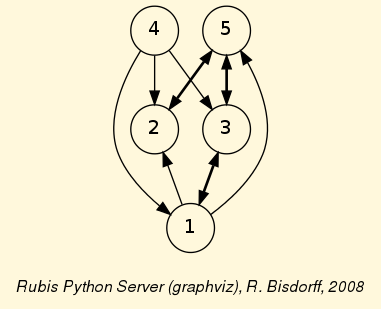
\includegraphics{randomValuationDigraph.png}

\end{fulllineitems}

\index{RandomWeakTournament (class in digraphs)}

\begin{fulllineitems}
\phantomsection\label{techDoc:digraphs.RandomWeakTournament}\pysiglinewithargsret{\strong{class }\code{digraphs.}\bfcode{RandomWeakTournament}}{\emph{order=10}, \emph{ndigits=2}, \emph{hasIntegerValuation=False}, \emph{weaknessDegree=0.25}, \emph{Comments=False}}{}
Bases: {\hyperref[techDoc:digraphs.Digraph]{\code{digraphs.Digraph}}}
\begin{description}
\item[{Parameter:}] \leavevmode
order = n \textgreater{} 0

\end{description}

Specialization of the general Digraph class for generating
temporary bipolar-valued weak tournaments

\end{fulllineitems}

\index{StrongComponentsCollapsedDigraph (class in digraphs)}

\begin{fulllineitems}
\phantomsection\label{techDoc:digraphs.StrongComponentsCollapsedDigraph}\pysiglinewithargsret{\strong{class }\code{digraphs.}\bfcode{StrongComponentsCollapsedDigraph}}{\emph{digraph=None}}{}
Bases: {\hyperref[techDoc:digraphs.Digraph]{\code{digraphs.Digraph}}}

Reduction of Digraph object to its strong components.
\index{showComponents() (digraphs.StrongComponentsCollapsedDigraph method)}

\begin{fulllineitems}
\phantomsection\label{techDoc:digraphs.StrongComponentsCollapsedDigraph.showComponents}\pysiglinewithargsret{\bfcode{showComponents}}{}{}
\end{fulllineitems}


\end{fulllineitems}

\index{SymmetricPartialDigraph (class in digraphs)}

\begin{fulllineitems}
\phantomsection\label{techDoc:digraphs.SymmetricPartialDigraph}\pysiglinewithargsret{\strong{class }\code{digraphs.}\bfcode{SymmetricPartialDigraph}}{\emph{digraph}}{}
Bases: {\hyperref[techDoc:digraphs.Digraph]{\code{digraphs.Digraph}}}

Renders the symmetric part of a Digraph instance.

..caution:

\begin{Verbatim}[commandchars=\\\{\}]
The not symmetric links of relationIn are all put to the meadian characteristics value!.
\end{Verbatim}

\end{fulllineitems}

\index{WeakCocaDigraph (class in digraphs)}

\begin{fulllineitems}
\phantomsection\label{techDoc:digraphs.WeakCocaDigraph}\pysiglinewithargsret{\strong{class }\code{digraphs.}\bfcode{WeakCocaDigraph}}{\emph{digraph=None}, \emph{comment=None}}{}
Bases: {\hyperref[techDoc:digraphs.Digraph]{\code{digraphs.Digraph}}}
\begin{description}
\item[{Parameters:}] \leavevmode
Stored or memory resident digraph instance.

\end{description}

Specialization of general Digraph class for instantiation
of weak chordless odd circuits augmented digraphs.
\index{addWeakCircuits() (digraphs.WeakCocaDigraph method)}

\begin{fulllineitems}
\phantomsection\label{techDoc:digraphs.WeakCocaDigraph.addWeakCircuits}\pysiglinewithargsret{\bfcode{addWeakCircuits}}{\emph{comment=None}}{}
Augmenting self with self.weakCircuits.

\end{fulllineitems}

\index{closureWeakChordlessOddCircuits() (digraphs.WeakCocaDigraph method)}

\begin{fulllineitems}
\phantomsection\label{techDoc:digraphs.WeakCocaDigraph.closureWeakChordlessOddCircuits}\pysiglinewithargsret{\bfcode{closureWeakChordlessOddCircuits}}{\emph{comment=None}}{}
Closure of cdordless odd circuits extraction.

\end{fulllineitems}

\index{showCircuits() (digraphs.WeakCocaDigraph method)}

\begin{fulllineitems}
\phantomsection\label{techDoc:digraphs.WeakCocaDigraph.showCircuits}\pysiglinewithargsret{\bfcode{showCircuits}}{}{}
show methods for chordless odd circuits in CocaGraph

\end{fulllineitems}


\end{fulllineitems}

\index{XMCDA2Digraph (class in digraphs)}

\begin{fulllineitems}
\phantomsection\label{techDoc:digraphs.XMCDA2Digraph}\pysiglinewithargsret{\strong{class }\code{digraphs.}\bfcode{XMCDA2Digraph}}{\emph{fileName='temp'}}{}
Bases: {\hyperref[techDoc:digraphs.Digraph]{\code{digraphs.Digraph}}}

Specialization of the general Digraph class for reading
stored XMCDA-2.0 formatted digraphs. Using the inbuilt module
xml.etree (for Python 2.5+).
\begin{description}
\item[{Param:}] \leavevmode
fileName (without the extension .xmcda).

\end{description}
\index{showAll() (digraphs.XMCDA2Digraph method)}

\begin{fulllineitems}
\phantomsection\label{techDoc:digraphs.XMCDA2Digraph.showAll}\pysiglinewithargsret{\bfcode{showAll}}{}{}
\end{fulllineitems}


\end{fulllineitems}

\index{XMCDADigraph (class in digraphs)}

\begin{fulllineitems}
\phantomsection\label{techDoc:digraphs.XMCDADigraph}\pysiglinewithargsret{\strong{class }\code{digraphs.}\bfcode{XMCDADigraph}}{\emph{fileName='temp'}}{}
Bases: {\hyperref[techDoc:digraphs.Digraph]{\code{digraphs.Digraph}}}

Specialization of the general Digraph class for reading
stored XMCDA formatted digraphs. Using the inbuilt module
xml.etree (for Python 2.5+).
\begin{description}
\item[{Param:}] \leavevmode
fileName (without the extension .xmcda).

\end{description}
\index{showAll() (digraphs.XMCDADigraph method)}

\begin{fulllineitems}
\phantomsection\label{techDoc:digraphs.XMCDADigraph.showAll}\pysiglinewithargsret{\bfcode{showAll}}{}{}
\end{fulllineitems}


\end{fulllineitems}

\index{XMLDigraph (class in digraphs)}

\begin{fulllineitems}
\phantomsection\label{techDoc:digraphs.XMLDigraph}\pysiglinewithargsret{\strong{class }\code{digraphs.}\bfcode{XMLDigraph}}{\emph{fileName='testsaveXML'}}{}
Bases: {\hyperref[techDoc:digraphs.Digraph]{\code{digraphs.Digraph}}}

Specialization of the general Digraph class for reading
stored XML formatted digraphs. Using the inbuilt module
xml.etree (for Python 2.5+).
\begin{description}
\item[{Param:}] \leavevmode
fileName (without the extension .xml).

\end{description}

\end{fulllineitems}

\index{XMLDigraph24 (class in digraphs)}

\begin{fulllineitems}
\phantomsection\label{techDoc:digraphs.XMLDigraph24}\pysiglinewithargsret{\strong{class }\code{digraphs.}\bfcode{XMLDigraph24}}{\emph{fileName='testsaveXML'}}{}
Bases: {\hyperref[techDoc:digraphs.Digraph]{\code{digraphs.Digraph}}}

Specialization of the general Digraph class for reading
stored XML formatted digraphs.
\index{showAll() (digraphs.XMLDigraph24 method)}

\begin{fulllineitems}
\phantomsection\label{techDoc:digraphs.XMLDigraph24.showAll}\pysiglinewithargsret{\bfcode{showAll}}{}{}
\end{fulllineitems}


\end{fulllineitems}

\index{XORDigraph (class in digraphs)}

\begin{fulllineitems}
\phantomsection\label{techDoc:digraphs.XORDigraph}\pysiglinewithargsret{\strong{class }\code{digraphs.}\bfcode{XORDigraph}}{\emph{d1}, \emph{d2}, \emph{Debug=False}}{}
Bases: {\hyperref[techDoc:digraphs.Digraph]{\code{digraphs.Digraph}}}

Instantiates the XOR digraph of two bipolar
digraphs d1 and d2 of same order.

\end{fulllineitems}

\index{all\_perms() (in module digraphs)}

\begin{fulllineitems}
\phantomsection\label{techDoc:digraphs.all_perms}\pysiglinewithargsret{\code{digraphs.}\bfcode{all\_perms}}{\emph{str}}{}
\end{fulllineitems}

\index{kChoicesDigraph (class in digraphs)}

\begin{fulllineitems}
\phantomsection\label{techDoc:digraphs.kChoicesDigraph}\pysiglinewithargsret{\strong{class }\code{digraphs.}\bfcode{kChoicesDigraph}}{\emph{digraph=None}, \emph{k=3}}{}
Bases: {\hyperref[techDoc:digraphs.Digraph]{\code{digraphs.Digraph}}}
\begin{description}
\item[{Parameters:}] \leavevmode
\begin{DUlineblock}{0em}
\item[] digraph := Stored or memory resident digraph instance
\item[] k := cardinality of the choices
\end{DUlineblock}

\end{description}

Specialization of general Digraph class for instantiation
of chordless odd circuits augmented digraphs.
\index{computeRelation() (digraphs.kChoicesDigraph method)}

\begin{fulllineitems}
\phantomsection\label{techDoc:digraphs.kChoicesDigraph.computeRelation}\pysiglinewithargsret{\bfcode{computeRelation}}{\emph{relation}}{}
computing the relation on kChoices

\end{fulllineitems}


\end{fulllineitems}

\index{powerset() (in module digraphs)}

\begin{fulllineitems}
\phantomsection\label{techDoc:digraphs.powerset}\pysiglinewithargsret{\code{digraphs.}\bfcode{powerset}}{\emph{S}}{}
Power set generator iterator.

Parameter S may be any object that is accepted as input by the set class constructor.

\end{fulllineitems}


Back to the {\hyperref[techDoc:technical-label]{\emph{Introduction}}}


\subsection{graphs module}
\label{techDoc:graphs-label}\label{techDoc:graphs-module}
A tutorial with coding examples is available here: {\hyperref[tutorial:graphs-tutorial-label]{\emph{Working with the graphs module}}}
\phantomsection\label{techDoc:module-graphs}\index{graphs (module)}\index{Graph (class in graphs)}

\begin{fulllineitems}
\phantomsection\label{techDoc:graphs.Graph}\pysiglinewithargsret{\strong{class }\code{graphs.}\bfcode{Graph}}{\emph{fileName=None}, \emph{Empty=False}, \emph{numberOfVertices=7}, \emph{edgeProbability=0.5}}{}
Bases: \code{builtins.object}

Graph class implementation with a vertices and an edges dictionary
and a gamma function (dictionary) from vertices to subsets of vertices.
\begin{description}
\item[{Example python3 session:}] \leavevmode
\begin{Verbatim}[commandchars=\\\{\}]
\PYG{g+gp}{\PYGZgt{}\PYGZgt{}\PYGZgt{} }\PYG{k+kn}{from} \PYG{n+nn}{graphs} \PYG{k+kn}{import} \PYG{n}{Graph}
\PYG{g+gp}{\PYGZgt{}\PYGZgt{}\PYGZgt{} }\PYG{n}{g} \PYG{o}{=} \PYG{n}{Graph}\PYG{p}{(}\PYG{n}{numberOfVertices}\PYG{o}{=}\PYG{l+m+mi}{5}\PYG{p}{,}\PYG{n}{edgeProbability}\PYG{o}{=}\PYG{l+m+mf}{0.5}\PYG{p}{)}
\PYG{g+gp}{\PYGZgt{}\PYGZgt{}\PYGZgt{} }\PYG{n}{g}\PYG{o}{.}\PYG{n}{showShort}\PYG{p}{(}\PYG{p}{)}
\PYG{g+go}{*\PYGZhy{}\PYGZhy{}\PYGZhy{}\PYGZhy{}\PYGZhy{} show short \PYGZhy{}\PYGZhy{}\PYGZhy{}\PYGZhy{}\PYGZhy{}\PYGZhy{}\PYGZhy{}\PYGZhy{}\PYGZhy{}\PYGZhy{}\PYGZhy{}\PYGZhy{}\PYGZhy{}\PYGZhy{}*}
\PYG{g+go}{*\PYGZhy{}\PYGZhy{}\PYGZhy{}\PYGZhy{} short description of the graph \PYGZhy{}\PYGZhy{}\PYGZhy{}\PYGZhy{}*}
\PYG{g+go}{Name             :  \PYGZsq{}random\PYGZsq{}}
\PYG{g+go}{Vertices         :  [\PYGZsq{}v1\PYGZsq{}, \PYGZsq{}v2\PYGZsq{}, \PYGZsq{}v3\PYGZsq{}, \PYGZsq{}v4\PYGZsq{}, \PYGZsq{}v5\PYGZsq{}]}
\PYG{g+go}{Valuation domain :  \PYGZob{}\PYGZsq{}med\PYGZsq{}: 0, \PYGZsq{}max\PYGZsq{}: 1, \PYGZsq{}min\PYGZsq{}: \PYGZhy{}1\PYGZcb{}}
\PYG{g+go}{Gamma function   :}
\PYG{g+go}{v1 \PYGZhy{}\PYGZgt{} [\PYGZsq{}v4\PYGZsq{}]}
\PYG{g+go}{v2 \PYGZhy{}\PYGZgt{} []}
\PYG{g+go}{v3 \PYGZhy{}\PYGZgt{} [\PYGZsq{}v4\PYGZsq{}]}
\PYG{g+go}{v4 \PYGZhy{}\PYGZgt{} [\PYGZsq{}v1\PYGZsq{}, \PYGZsq{}v3\PYGZsq{}]}
\PYG{g+go}{v5 \PYGZhy{}\PYGZgt{} []}
\end{Verbatim}

\end{description}
\index{chordlessPaths() (graphs.Graph method)}

\begin{fulllineitems}
\phantomsection\label{techDoc:graphs.Graph.chordlessPaths}\pysiglinewithargsret{\bfcode{chordlessPaths}}{\emph{Pk}, \emph{v0}, \emph{Comments=False}, \emph{Debug=False}}{}~\begin{description}
\item[{recursice chordless precycle (len \textgreater{} 3) construction:}] \leavevmode
Pk is the current pre chordless cycle
v0 is the initial vertex of the precycle
vn is the last vertex of the precycle

\end{description}

\end{fulllineitems}

\index{computeChordlessCycles() (graphs.Graph method)}

\begin{fulllineitems}
\phantomsection\label{techDoc:graphs.Graph.computeChordlessCycles}\pysiglinewithargsret{\bfcode{computeChordlessCycles}}{\emph{Comments=True}, \emph{Debug=False}}{}
Renders the set of all chordless cycles observed in a Graph
intance.

\end{fulllineitems}

\index{depthFirstSearch() (graphs.Graph method)}

\begin{fulllineitems}
\phantomsection\label{techDoc:graphs.Graph.depthFirstSearch}\pysiglinewithargsret{\bfcode{depthFirstSearch}}{\emph{Debug=False}}{}
Depth first search through a graph

\end{fulllineitems}

\index{exportGraphViz() (graphs.Graph method)}

\begin{fulllineitems}
\phantomsection\label{techDoc:graphs.Graph.exportGraphViz}\pysiglinewithargsret{\bfcode{exportGraphViz}}{\emph{fileName=None}, \emph{noSilent=True}, \emph{graphType='png'}, \emph{graphSize=`7}, \emph{7'}}{}
Exports GraphViz dot file  for graph drawing filtering.
\begin{description}
\item[{Example:}] \leavevmode
\begin{Verbatim}[commandchars=\\\{\}]
\PYG{g+gp}{\PYGZgt{}\PYGZgt{}\PYGZgt{} }\PYG{n}{g} \PYG{o}{=} \PYG{n}{Graph}\PYG{p}{(}\PYG{n}{numberOfVertices}\PYG{o}{=}\PYG{l+m+mi}{5}\PYG{p}{,}\PYG{n}{edgeProbability}\PYG{o}{=}\PYG{l+m+mf}{0.3}\PYG{p}{)}
\PYG{g+gp}{\PYGZgt{}\PYGZgt{}\PYGZgt{} }\PYG{n}{g}\PYG{o}{.}\PYG{n}{exportGraphViz}\PYG{p}{(}\PYG{l+s}{\PYGZsq{}}\PYG{l+s}{randomGraph}\PYG{l+s}{\PYGZsq{}}\PYG{p}{)}\PYG{p}{)}
\end{Verbatim}

\end{description}

{\hfill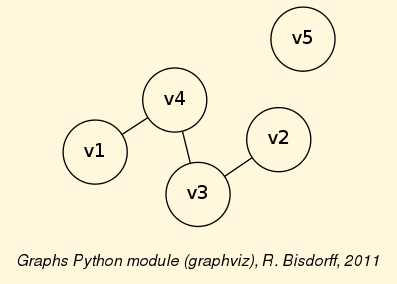
\includegraphics{randomGraph.png}\hfill}

\end{fulllineitems}

\index{gammaSets() (graphs.Graph method)}

\begin{fulllineitems}
\phantomsection\label{techDoc:graphs.Graph.gammaSets}\pysiglinewithargsret{\bfcode{gammaSets}}{\emph{Debug=False}}{}
renders the gamma function as dictionary

\end{fulllineitems}

\index{graph2Digraph() (graphs.Graph method)}

\begin{fulllineitems}
\phantomsection\label{techDoc:graphs.Graph.graph2Digraph}\pysiglinewithargsret{\bfcode{graph2Digraph}}{}{}
Converts a Graph object into a Digraph object.

\end{fulllineitems}

\index{save() (graphs.Graph method)}

\begin{fulllineitems}
\phantomsection\label{techDoc:graphs.Graph.save}\pysiglinewithargsret{\bfcode{save}}{\emph{fileName='tempGraph'}, \emph{Debug=False}}{}
Persistent storage of a Graph class instance in the form of a python source code file.

\end{fulllineitems}

\index{saveEdges() (graphs.Graph method)}

\begin{fulllineitems}
\phantomsection\label{techDoc:graphs.Graph.saveEdges}\pysiglinewithargsret{\bfcode{saveEdges}}{\emph{fileName='graphEdges'}, \emph{Agrum=False}, \emph{Decimal=True}}{}
Saving graph instances as list of edges, ie node node on each line
for enumChordlessCycles C++/agrum progam.

\end{fulllineitems}

\index{showShort() (graphs.Graph method)}

\begin{fulllineitems}
\phantomsection\label{techDoc:graphs.Graph.showShort}\pysiglinewithargsret{\bfcode{showShort}}{}{}
Generic show method for Graph instances.

\end{fulllineitems}


\end{fulllineitems}

\index{GridGraph (class in graphs)}

\begin{fulllineitems}
\phantomsection\label{techDoc:graphs.GridGraph}\pysiglinewithargsret{\strong{class }\code{graphs.}\bfcode{GridGraph}}{\emph{n=5}, \emph{m=5}, \emph{valuationMin=-1}, \emph{valuationMax=1}}{}
Bases: {\hyperref[techDoc:graphs.Graph]{\code{graphs.Graph}}}

Specialization of the general Graph class for generating
temporary Grid graphs of dimension n times m.
\begin{description}
\item[{\emph{Parameters}:}] \leavevmode\begin{itemize}
\item {} 
n,m \textgreater{} 0

\item {} 
valuationDomain =\{`min':m, `max':M\}

\end{itemize}

\item[{Default instantiation (5 times 5 Grid Digraph):}] \leavevmode\begin{itemize}
\item {} 
n = 5,

\item {} 
m=5,

\item {} 
valuationDomain = \{`min':-1.0,'max':1.0\}.

\end{itemize}

\end{description}

Example of 5x5 GridGraph instance:

{\hfill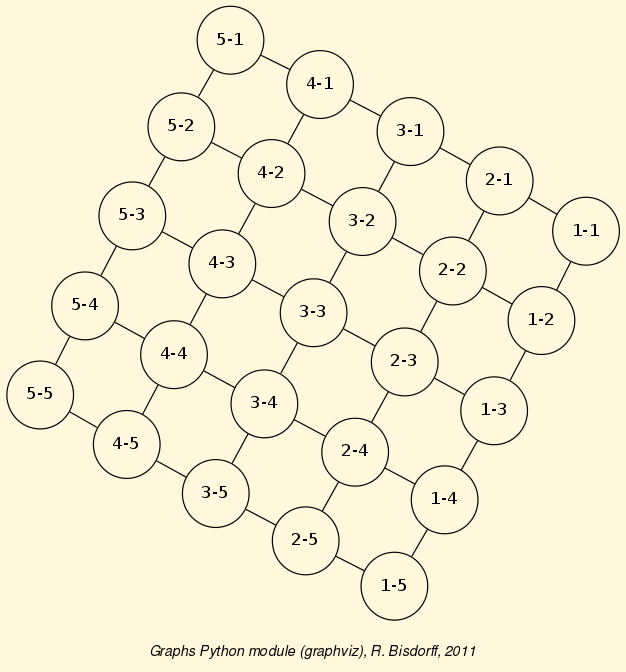
\includegraphics{grid-5-5.png}\hfill}
\index{showShort() (graphs.GridGraph method)}

\begin{fulllineitems}
\phantomsection\label{techDoc:graphs.GridGraph.showShort}\pysiglinewithargsret{\bfcode{showShort}}{}{}
\end{fulllineitems}


\end{fulllineitems}

\index{IsingModel (class in graphs)}

\begin{fulllineitems}
\phantomsection\label{techDoc:graphs.IsingModel}\pysiglinewithargsret{\strong{class }\code{graphs.}\bfcode{IsingModel}}{\emph{g}, \emph{beta=0}, \emph{nSim=None}, \emph{Debug=False}}{}
Bases: {\hyperref[techDoc:graphs.Graph]{\code{graphs.Graph}}}

Specialisation of a Gibbs Sampler for the Ising model
\begin{description}
\item[{Example:}] \leavevmode
\begin{Verbatim}[commandchars=\\\{\}]
\PYG{g+gp}{\PYGZgt{}\PYGZgt{}\PYGZgt{} }\PYG{n}{g} \PYG{o}{=} \PYG{n}{GridGraph}\PYG{p}{(}\PYG{n}{n}\PYG{o}{=}\PYG{l+m+mi}{15}\PYG{p}{,}\PYG{n}{m}\PYG{o}{=}\PYG{l+m+mi}{15}\PYG{p}{)}
\PYG{g+gp}{\PYGZgt{}\PYGZgt{}\PYGZgt{} }\PYG{n}{g}\PYG{o}{.}\PYG{n}{showShort}\PYG{p}{(}\PYG{p}{)}
\PYG{g+go}{*\PYGZhy{}\PYGZhy{}\PYGZhy{}\PYGZhy{}\PYGZhy{} show short \PYGZhy{}\PYGZhy{}\PYGZhy{}\PYGZhy{}\PYGZhy{}\PYGZhy{}\PYGZhy{}\PYGZhy{}\PYGZhy{}\PYGZhy{}\PYGZhy{}\PYGZhy{}\PYGZhy{}\PYGZhy{}*}
\PYG{g+go}{Grid graph    :  grid\PYGZhy{}6\PYGZhy{}6}
\PYG{g+go}{n             :  6}
\PYG{g+go}{m             :  6}
\PYG{g+go}{order         :  36}
\PYG{g+gp}{\PYGZgt{}\PYGZgt{}\PYGZgt{} }\PYG{n}{im} \PYG{o}{=} \PYG{n}{IsingModel}\PYG{p}{(}\PYG{n}{g}\PYG{p}{,}\PYG{n}{beta}\PYG{o}{=}\PYG{l+m+mf}{0.3}\PYG{p}{,}\PYG{n}{nSim}\PYG{o}{=}\PYG{l+m+mi}{100000}\PYG{p}{,}\PYG{n}{Debug}\PYG{o}{=}\PYG{n+nb+bp}{False}\PYG{p}{)}
\PYG{g+go}{Running a Gibbs Sampler for 100000 step !}
\PYG{g+gp}{\PYGZgt{}\PYGZgt{}\PYGZgt{} }\PYG{n}{im}\PYG{o}{.}\PYG{n}{exportGraphViz}\PYG{p}{(}\PYG{n}{colors}\PYG{o}{=}\PYG{p}{[}\PYG{l+s}{\PYGZsq{}}\PYG{l+s}{lightblue}\PYG{l+s}{\PYGZsq{}}\PYG{p}{,}\PYG{l+s}{\PYGZsq{}}\PYG{l+s}{lightcoral}\PYG{l+s}{\PYGZsq{}}\PYG{p}{]}\PYG{p}{)}
\PYG{g+go}{*\PYGZhy{}\PYGZhy{}\PYGZhy{}\PYGZhy{} exporting a dot file for GraphViz tools \PYGZhy{}\PYGZhy{}\PYGZhy{}\PYGZhy{}\PYGZhy{}\PYGZhy{}\PYGZhy{}\PYGZhy{}\PYGZhy{}*}
\PYG{g+go}{Exporting to grid\PYGZhy{}15\PYGZhy{}15\PYGZhy{}ising.dot}
\PYG{g+go}{fdp \PYGZhy{}Tpng grid\PYGZhy{}15\PYGZhy{}15\PYGZhy{}ising.dot \PYGZhy{}o grid\PYGZhy{}15\PYGZhy{}15\PYGZhy{}ising.png}
\end{Verbatim}

\end{description}

{\hfill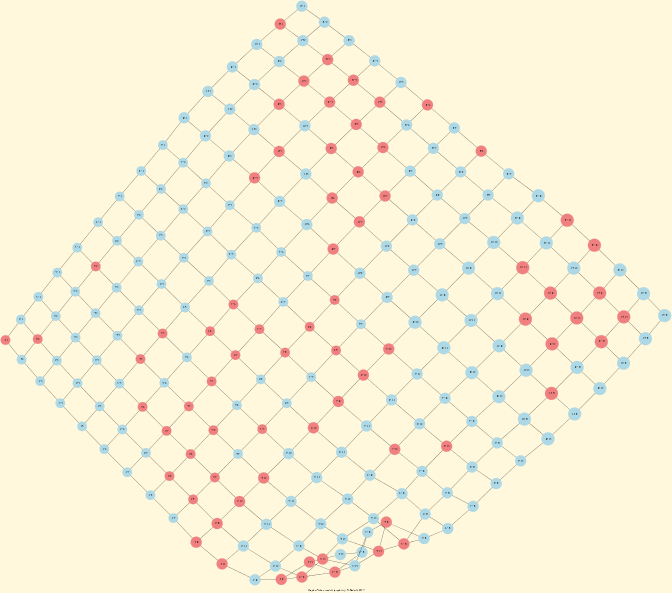
\includegraphics{grid-15-15-ising.png}\hfill}
\index{computeSpinEnergy() (graphs.IsingModel method)}

\begin{fulllineitems}
\phantomsection\label{techDoc:graphs.IsingModel.computeSpinEnergy}\pysiglinewithargsret{\bfcode{computeSpinEnergy}}{}{}
Spin energy H(c) of a spin configuration is
H(c) = -sum\_\{\{x,y\} in self.edges\}{[}spin\_c(x)*spin\_c(y){]}

\end{fulllineitems}

\index{exportGraphViz() (graphs.IsingModel method)}

\begin{fulllineitems}
\phantomsection\label{techDoc:graphs.IsingModel.exportGraphViz}\pysiglinewithargsret{\bfcode{exportGraphViz}}{\emph{fileName=None, noSilent=True, graphType='png', graphSize=`7,7', edgeColor='black', colors={[}'gold', `lightblue'{]}}}{}
Exports GraphViz dot file  for Ising models drawing filtering.

\end{fulllineitems}

\index{generateSpinConfiguration() (graphs.IsingModel method)}

\begin{fulllineitems}
\phantomsection\label{techDoc:graphs.IsingModel.generateSpinConfiguration}\pysiglinewithargsret{\bfcode{generateSpinConfiguration}}{\emph{beta=0}, \emph{nSim=None}, \emph{Debug=False}}{}
\end{fulllineitems}


\end{fulllineitems}

\index{MISModel (class in graphs)}

\begin{fulllineitems}
\phantomsection\label{techDoc:graphs.MISModel}\pysiglinewithargsret{\strong{class }\code{graphs.}\bfcode{MISModel}}{\emph{g}, \emph{nSim=None}, \emph{maxIter=20}, \emph{Debug=False}}{}
Bases: {\hyperref[techDoc:graphs.Graph]{\code{graphs.Graph}}}

Specialisation of a Gibbs Sampler for the hard code model,
that is a random MIS generator.
\begin{description}
\item[{Example:}] \leavevmode
\begin{Verbatim}[commandchars=\\\{\}]
\PYG{g+gp}{\PYGZgt{}\PYGZgt{}\PYGZgt{} }\PYG{k+kn}{from} \PYG{n+nn}{digraphs} \PYG{k+kn}{import} \PYG{n}{CirculantDigraph}        
\PYG{g+gp}{\PYGZgt{}\PYGZgt{}\PYGZgt{} }\PYG{n}{dg} \PYG{o}{=} \PYG{n}{CirculantDigraph}\PYG{p}{(}\PYG{n}{order}\PYG{o}{=}\PYG{l+m+mi}{15}\PYG{p}{)}
\PYG{g+gp}{\PYGZgt{}\PYGZgt{}\PYGZgt{} }\PYG{n}{g} \PYG{o}{=} \PYG{n}{dg}\PYG{o}{.}\PYG{n}{digraph2Graph}\PYG{p}{(}\PYG{p}{)}
\PYG{g+gp}{\PYGZgt{}\PYGZgt{}\PYGZgt{} }\PYG{n}{g}\PYG{o}{.}\PYG{n}{showShort}\PYG{p}{(}\PYG{p}{)}
\PYG{g+go}{*\PYGZhy{}\PYGZhy{}\PYGZhy{}\PYGZhy{} short description of the graph \PYGZhy{}\PYGZhy{}\PYGZhy{}\PYGZhy{}*}
\PYG{g+go}{Name             : \PYGZsq{}c15\PYGZsq{}}
\PYG{g+go}{Vertices         :  [\PYGZsq{}1\PYGZsq{}, \PYGZsq{}10\PYGZsq{}, \PYGZsq{}11\PYGZsq{}, \PYGZsq{}12\PYGZsq{}, \PYGZsq{}13\PYGZsq{}, \PYGZsq{}14\PYGZsq{},}
\PYG{g+go}{                     \PYGZsq{}15\PYGZsq{}, \PYGZsq{}2\PYGZsq{}, \PYGZsq{}3\PYGZsq{}, \PYGZsq{}4\PYGZsq{}, \PYGZsq{}5\PYGZsq{}, \PYGZsq{}6\PYGZsq{}, \PYGZsq{}7\PYGZsq{},}
\PYG{g+go}{                     \PYGZsq{}8\PYGZsq{}, \PYGZsq{}9\PYGZsq{}]}
\PYG{g+go}{Valuation domain :  \PYGZob{}\PYGZsq{}med\PYGZsq{}: 0, \PYGZsq{}min\PYGZsq{}: \PYGZhy{}1, \PYGZsq{}max\PYGZsq{}: 1\PYGZcb{}}
\PYG{g+go}{Gamma function   : }
\PYG{g+go}{1 \PYGZhy{}\PYGZgt{} [\PYGZsq{}2\PYGZsq{}, \PYGZsq{}15\PYGZsq{}]}
\PYG{g+go}{10 \PYGZhy{}\PYGZgt{} [\PYGZsq{}11\PYGZsq{}, \PYGZsq{}9\PYGZsq{}]}
\PYG{g+go}{11 \PYGZhy{}\PYGZgt{} [\PYGZsq{}10\PYGZsq{}, \PYGZsq{}12\PYGZsq{}]}
\PYG{g+go}{12 \PYGZhy{}\PYGZgt{} [\PYGZsq{}13\PYGZsq{}, \PYGZsq{}11\PYGZsq{}]}
\PYG{g+go}{13 \PYGZhy{}\PYGZgt{} [\PYGZsq{}12\PYGZsq{}, \PYGZsq{}14\PYGZsq{}]}
\PYG{g+go}{14 \PYGZhy{}\PYGZgt{} [\PYGZsq{}15\PYGZsq{}, \PYGZsq{}13\PYGZsq{}]}
\PYG{g+go}{15 \PYGZhy{}\PYGZgt{} [\PYGZsq{}1\PYGZsq{}, \PYGZsq{}14\PYGZsq{}]}
\PYG{g+go}{2 \PYGZhy{}\PYGZgt{} [\PYGZsq{}1\PYGZsq{}, \PYGZsq{}3\PYGZsq{}]}
\PYG{g+go}{3 \PYGZhy{}\PYGZgt{} [\PYGZsq{}2\PYGZsq{}, \PYGZsq{}4\PYGZsq{}]}
\PYG{g+go}{4 \PYGZhy{}\PYGZgt{} [\PYGZsq{}3\PYGZsq{}, \PYGZsq{}5\PYGZsq{}]}
\PYG{g+go}{5 \PYGZhy{}\PYGZgt{} [\PYGZsq{}6\PYGZsq{}, \PYGZsq{}4\PYGZsq{}]}
\PYG{g+go}{6 \PYGZhy{}\PYGZgt{} [\PYGZsq{}7\PYGZsq{}, \PYGZsq{}5\PYGZsq{}]}
\PYG{g+go}{7 \PYGZhy{}\PYGZgt{} [\PYGZsq{}6\PYGZsq{}, \PYGZsq{}8\PYGZsq{}]}
\PYG{g+go}{8 \PYGZhy{}\PYGZgt{} [\PYGZsq{}7\PYGZsq{}, \PYGZsq{}9\PYGZsq{}]}
\PYG{g+go}{9 \PYGZhy{}\PYGZgt{} [\PYGZsq{}10\PYGZsq{}, \PYGZsq{}8\PYGZsq{}]}
\PYG{g+gp}{\PYGZgt{}\PYGZgt{}\PYGZgt{} }\PYG{n}{mis} \PYG{o}{=} \PYG{n}{MISModel}\PYG{p}{(}\PYG{n}{g}\PYG{p}{)}
\PYG{g+go}{Running a Gibbs Sampler for 1050 step !}
\PYG{g+gp}{\PYGZgt{}\PYGZgt{}\PYGZgt{} }\PYG{n}{mis}\PYG{o}{.}\PYG{n}{checkMIS}\PYG{p}{(}\PYG{p}{)}
\PYG{g+go}{\PYGZob{}\PYGZsq{}2\PYGZsq{},\PYGZsq{}4\PYGZsq{},\PYGZsq{}7\PYGZsq{},\PYGZsq{}9\PYGZsq{},\PYGZsq{}11\PYGZsq{},\PYGZsq{}13\PYGZsq{},\PYGZsq{}15\PYGZsq{}\PYGZcb{}  is maximal !}
\PYG{g+gp}{\PYGZgt{}\PYGZgt{}\PYGZgt{} }\PYG{n}{mis}\PYG{o}{.}\PYG{n}{exportGraphViz}\PYG{p}{(}\PYG{p}{)}
\PYG{g+go}{*\PYGZhy{}\PYGZhy{}\PYGZhy{}\PYGZhy{} exporting a dot file for GraphViz tools \PYGZhy{}\PYGZhy{}\PYGZhy{}\PYGZhy{}\PYGZhy{}\PYGZhy{}\PYGZhy{}\PYGZhy{}\PYGZhy{}*}
\PYG{g+go}{Exporting to c15\PYGZhy{}mis.dot}
\PYG{g+go}{fdp \PYGZhy{}Tpng c15\PYGZhy{}mis.dot \PYGZhy{}o c15\PYGZhy{}mis.png}
\end{Verbatim}

\end{description}

{\hfill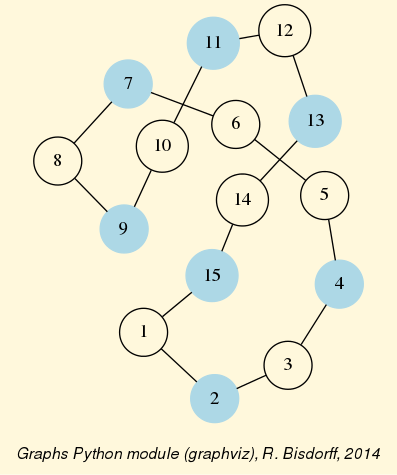
\includegraphics{c15-mis.png}\hfill}
\index{checkMIS() (graphs.MISModel method)}

\begin{fulllineitems}
\phantomsection\label{techDoc:graphs.MISModel.checkMIS}\pysiglinewithargsret{\bfcode{checkMIS}}{\emph{Comments=True}}{}
Verify maximality of independent set.

\begin{notice}{note}{Note:}
Returns three sets: an independent choice,
the covered vertices, and the remaining uncovered vertices.
When the last set is empty, the independent choice is maximal.
\end{notice}

\end{fulllineitems}

\index{exportGraphViz() (graphs.MISModel method)}

\begin{fulllineitems}
\phantomsection\label{techDoc:graphs.MISModel.exportGraphViz}\pysiglinewithargsret{\bfcode{exportGraphViz}}{\emph{fileName=None}, \emph{noSilent=True}, \emph{graphType='png'}, \emph{graphSize=`7}, \emph{7'}, \emph{misColor='lightblue'}}{}
Exports GraphViz dot file  for MIS models drawing filtering.

\end{fulllineitems}

\index{generateMIS() (graphs.MISModel method)}

\begin{fulllineitems}
\phantomsection\label{techDoc:graphs.MISModel.generateMIS}\pysiglinewithargsret{\bfcode{generateMIS}}{\emph{Reset=True}, \emph{nSim=None}, \emph{Comments=True}, \emph{Debug=False}}{}
\end{fulllineitems}


\end{fulllineitems}

\index{MetropolisChain (class in graphs)}

\begin{fulllineitems}
\phantomsection\label{techDoc:graphs.MetropolisChain}\pysiglinewithargsret{\strong{class }\code{graphs.}\bfcode{MetropolisChain}}{\emph{g}, \emph{probs=None}}{}
Bases: {\hyperref[techDoc:graphs.Graph]{\code{graphs.Graph}}}

Specialisation of the graph class for implementing a generic
Metropolis Markov Chain Monte Carlo sampler with a given probability distribution
probs = \{`v1': x, `v2': y, ...\}
\begin{description}
\item[{Usage example:}] \leavevmode
\begin{Verbatim}[commandchars=\\\{\}]
\PYG{g+gp}{\PYGZgt{}\PYGZgt{}\PYGZgt{} }\PYG{n}{g} \PYG{o}{=} \PYG{n}{Graph}\PYG{p}{(}\PYG{n}{numberOfVertices}\PYG{o}{=}\PYG{l+m+mi}{5}\PYG{p}{,}\PYG{n}{edgeProbability}\PYG{o}{=}\PYG{l+m+mf}{0.5}\PYG{p}{)}
\PYG{g+gp}{\PYGZgt{}\PYGZgt{}\PYGZgt{} }\PYG{n}{g}\PYG{o}{.}\PYG{n}{showShort}\PYG{p}{(}\PYG{p}{)}
\PYG{g+go}{*\PYGZhy{}\PYGZhy{}\PYGZhy{}\PYGZhy{} short description of the graph \PYGZhy{}\PYGZhy{}\PYGZhy{}\PYGZhy{}*}
\PYG{g+go}{Name             : \PYGZsq{}randomGraph\PYGZsq{}}
\PYG{g+go}{Vertices         :  [\PYGZsq{}v1\PYGZsq{}, \PYGZsq{}v2\PYGZsq{}, \PYGZsq{}v3\PYGZsq{}, \PYGZsq{}v4\PYGZsq{}, \PYGZsq{}v5\PYGZsq{}]}
\PYG{g+go}{Valuation domain :  \PYGZob{}\PYGZsq{}max\PYGZsq{}: 1, \PYGZsq{}med\PYGZsq{}: 0, \PYGZsq{}min\PYGZsq{}: \PYGZhy{}1\PYGZcb{}}
\PYG{g+go}{Gamma function   : }
\PYG{g+go}{v1 \PYGZhy{}\PYGZgt{} [\PYGZsq{}v2\PYGZsq{}, \PYGZsq{}v3\PYGZsq{}, \PYGZsq{}v4\PYGZsq{}]}
\PYG{g+go}{v2 \PYGZhy{}\PYGZgt{} [\PYGZsq{}v1\PYGZsq{}, \PYGZsq{}v4\PYGZsq{}]}
\PYG{g+go}{v3 \PYGZhy{}\PYGZgt{} [\PYGZsq{}v5\PYGZsq{}, \PYGZsq{}v1\PYGZsq{}]}
\PYG{g+go}{v4 \PYGZhy{}\PYGZgt{} [\PYGZsq{}v2\PYGZsq{}, \PYGZsq{}v5\PYGZsq{}, \PYGZsq{}v1\PYGZsq{}]}
\PYG{g+go}{v5 \PYGZhy{}\PYGZgt{} [\PYGZsq{}v3\PYGZsq{}, \PYGZsq{}v4\PYGZsq{}]        }
\PYG{g+gp}{\PYGZgt{}\PYGZgt{}\PYGZgt{} }\PYG{n}{probs} \PYG{o}{=} \PYG{p}{\PYGZob{}}\PYG{p}{\PYGZcb{}}
\PYG{g+gp}{\PYGZgt{}\PYGZgt{}\PYGZgt{} }\PYG{n}{n} \PYG{o}{=} \PYG{n}{g}\PYG{o}{.}\PYG{n}{order}
\PYG{g+gp}{\PYGZgt{}\PYGZgt{}\PYGZgt{} }\PYG{n}{i} \PYG{o}{=} \PYG{l+m+mi}{0}
\PYG{g+gp}{\PYGZgt{}\PYGZgt{}\PYGZgt{} }\PYG{n}{verticesList} \PYG{o}{=} \PYG{p}{[}\PYG{n}{x} \PYG{k}{for} \PYG{n}{x} \PYG{o+ow}{in} \PYG{n}{g}\PYG{o}{.}\PYG{n}{vertices}\PYG{p}{]}
\PYG{g+gp}{\PYGZgt{}\PYGZgt{}\PYGZgt{} }\PYG{n}{verticesList}\PYG{o}{.}\PYG{n}{sort}\PYG{p}{(}\PYG{p}{)}
\PYG{g+gp}{\PYGZgt{}\PYGZgt{}\PYGZgt{} }\PYG{k}{for} \PYG{n}{v} \PYG{o+ow}{in} \PYG{n}{verticesList}\PYG{p}{:}
\PYG{g+gp}{... }    \PYG{n}{probs}\PYG{p}{[}\PYG{n}{v}\PYG{p}{]} \PYG{o}{=} \PYG{p}{(}\PYG{n}{n} \PYG{o}{\PYGZhy{}} \PYG{n}{i}\PYG{p}{)}\PYG{o}{/}\PYG{p}{(}\PYG{n}{n}\PYG{o}{*}\PYG{p}{(}\PYG{n}{n}\PYG{o}{+}\PYG{l+m+mi}{1}\PYG{p}{)}\PYG{o}{/}\PYG{l+m+mi}{2}\PYG{p}{)}
\PYG{g+gp}{... }    \PYG{n}{i} \PYG{o}{+}\PYG{o}{=} \PYG{l+m+mi}{1}
\PYG{g+gp}{\PYGZgt{}\PYGZgt{}\PYGZgt{} }\PYG{n}{met} \PYG{o}{=} \PYG{n}{MetropolisChain}\PYG{p}{(}\PYG{n}{g}\PYG{p}{,}\PYG{n}{probs}\PYG{p}{)}
\PYG{g+gp}{\PYGZgt{}\PYGZgt{}\PYGZgt{} }\PYG{n}{frequency} \PYG{o}{=} \PYG{n}{met}\PYG{o}{.}\PYG{n}{checkSampling}\PYG{p}{(}\PYG{n}{verticesList}\PYG{p}{[}\PYG{l+m+mi}{0}\PYG{p}{]}\PYG{p}{,}\PYG{n}{nSim}\PYG{o}{=}\PYG{l+m+mi}{30000}\PYG{p}{)}
\PYG{g+gp}{\PYGZgt{}\PYGZgt{}\PYGZgt{} }\PYG{k}{for} \PYG{n}{v} \PYG{o+ow}{in} \PYG{n}{verticesList}\PYG{p}{:}
\PYG{g+gp}{... }    \PYG{k}{print}\PYG{p}{(}\PYG{n}{v}\PYG{p}{,}\PYG{n}{probs}\PYG{p}{[}\PYG{n}{v}\PYG{p}{]}\PYG{p}{,}\PYG{n}{frequency}\PYG{p}{[}\PYG{n}{v}\PYG{p}{]}\PYG{p}{)}
\PYG{g+go}{v1 0.3333 0.3343}
\PYG{g+go}{v2 0.2666 0.2680}
\PYG{g+go}{v3 0.2    0.2030 }
\PYG{g+go}{v4 0.1333 0.1311}
\PYG{g+go}{v5 0.0666 0.0635}
\PYG{g+gp}{\PYGZgt{}\PYGZgt{}\PYGZgt{} }\PYG{n}{met}\PYG{o}{.}\PYG{n}{showTransitionMatrix}\PYG{p}{(}\PYG{p}{)}
\PYG{g+go}{* \PYGZhy{}\PYGZhy{}\PYGZhy{}\PYGZhy{} Transition Matrix \PYGZhy{}\PYGZhy{}\PYGZhy{}\PYGZhy{}\PYGZhy{}}
\PYG{g+go}{  Pij  \textbar{} \PYGZsq{}v1\PYGZsq{}    \PYGZsq{}v2\PYGZsq{}    \PYGZsq{}v3\PYGZsq{}    \PYGZsq{}v4\PYGZsq{}    \PYGZsq{}v5\PYGZsq{}     }
\PYG{g+go}{  \PYGZhy{}\PYGZhy{}\PYGZhy{}\PYGZhy{}\PYGZhy{}\textbar{}\PYGZhy{}\PYGZhy{}\PYGZhy{}\PYGZhy{}\PYGZhy{}\PYGZhy{}\PYGZhy{}\PYGZhy{}\PYGZhy{}\PYGZhy{}\PYGZhy{}\PYGZhy{}\PYGZhy{}\PYGZhy{}\PYGZhy{}\PYGZhy{}\PYGZhy{}\PYGZhy{}\PYGZhy{}\PYGZhy{}\PYGZhy{}\PYGZhy{}\PYGZhy{}\PYGZhy{}\PYGZhy{}\PYGZhy{}\PYGZhy{}\PYGZhy{}\PYGZhy{}\PYGZhy{}\PYGZhy{}\PYGZhy{}\PYGZhy{}\PYGZhy{}\PYGZhy{}\PYGZhy{}\PYGZhy{}}
\PYG{g+go}{  \PYGZsq{}v1\PYGZsq{} \textbar{}  0.23   0.33    0.30    0.13    0.00    }
\PYG{g+go}{  \PYGZsq{}v2\PYGZsq{} \textbar{}  0.42   0.42    0.00    0.17    0.00    }
\PYG{g+go}{  \PYGZsq{}v3\PYGZsq{} \textbar{}  0.50   0.00    0.33    0.00    0.17    }
\PYG{g+go}{  \PYGZsq{}v4\PYGZsq{} \textbar{}  0.33   0.33    0.00    0.08    0.25    }
\PYG{g+go}{  \PYGZsq{}v5\PYGZsq{} \textbar{}  0.00   0.00    0.50    0.50    0.00    }
\end{Verbatim}

\end{description}
\index{MCMCtransition() (graphs.MetropolisChain method)}

\begin{fulllineitems}
\phantomsection\label{techDoc:graphs.MetropolisChain.MCMCtransition}\pysiglinewithargsret{\bfcode{MCMCtransition}}{\emph{si}, \emph{Debug=False}}{}
\end{fulllineitems}

\index{checkSampling() (graphs.MetropolisChain method)}

\begin{fulllineitems}
\phantomsection\label{techDoc:graphs.MetropolisChain.checkSampling}\pysiglinewithargsret{\bfcode{checkSampling}}{\emph{si}, \emph{nSim}}{}
\end{fulllineitems}

\index{computeTransitionMatrix() (graphs.MetropolisChain method)}

\begin{fulllineitems}
\phantomsection\label{techDoc:graphs.MetropolisChain.computeTransitionMatrix}\pysiglinewithargsret{\bfcode{computeTransitionMatrix}}{}{}
\end{fulllineitems}

\index{saveCSVTransition() (graphs.MetropolisChain method)}

\begin{fulllineitems}
\phantomsection\label{techDoc:graphs.MetropolisChain.saveCSVTransition}\pysiglinewithargsret{\bfcode{saveCSVTransition}}{\emph{fileName='transition'}, \emph{Debug=False}}{}
Persistent storage of the transition matrix in the form of
a csv file.

\end{fulllineitems}

\index{showTransitionMatrix() (graphs.MetropolisChain method)}

\begin{fulllineitems}
\phantomsection\label{techDoc:graphs.MetropolisChain.showTransitionMatrix}\pysiglinewithargsret{\bfcode{showTransitionMatrix}}{\emph{Sorted=True}, \emph{IntegerValues=False}, \emph{vertices=None}, \emph{relation=None}, \emph{ndigits=2}, \emph{ReflexiveTerms=True}}{}
Prints on stdout the transition probabilities in
vertices X vertices table format.

\end{fulllineitems}


\end{fulllineitems}

\index{Q\_Coloring (class in graphs)}

\begin{fulllineitems}
\phantomsection\label{techDoc:graphs.Q_Coloring}\pysiglinewithargsret{\strong{class }\code{graphs.}\bfcode{Q\_Coloring}}{\emph{g, colors={[}'gold', `lightcoral', `lightblue'{]}, nSim=None, maxIter=20, Comments=True, Debug=False}}{}
Bases: {\hyperref[techDoc:graphs.Graph]{\code{graphs.Graph}}}

Generate a q-coloring of a Graph instance via a Gibbs MCMC sampler in
nSim simulation steps (default = len(graph.edges)).
\begin{quote}
\begin{description}
\item[{Example 3-coloring of a grid 6x6 :}] \leavevmode
\begin{Verbatim}[commandchars=\\\{\}]
\PYG{g+gp}{\PYGZgt{}\PYGZgt{}\PYGZgt{} }\PYG{n}{g} \PYG{o}{=} \PYG{n}{GridGraph}\PYG{p}{(}\PYG{n}{n}\PYG{o}{=}\PYG{l+m+mi}{6}\PYG{p}{,}\PYG{n}{m}\PYG{o}{=}\PYG{l+m+mi}{6}\PYG{p}{)}
\PYG{g+gp}{\PYGZgt{}\PYGZgt{}\PYGZgt{} }\PYG{n}{g}\PYG{o}{.}\PYG{n}{showShort}\PYG{p}{(}\PYG{p}{)}
\PYG{g+gp}{\PYGZgt{}\PYGZgt{}\PYGZgt{} }\PYG{n}{g}\PYG{o}{.}\PYG{n}{exportGraphViz}\PYG{p}{(}\PYG{p}{)}
\PYG{g+go}{*\PYGZhy{}\PYGZhy{}\PYGZhy{}\PYGZhy{}\PYGZhy{} show short \PYGZhy{}\PYGZhy{}\PYGZhy{}\PYGZhy{}\PYGZhy{}\PYGZhy{}\PYGZhy{}\PYGZhy{}\PYGZhy{}\PYGZhy{}\PYGZhy{}\PYGZhy{}\PYGZhy{}\PYGZhy{}*}
\PYG{g+go}{Grid graph    :  grid\PYGZhy{}6\PYGZhy{}6}
\PYG{g+go}{n             :  6}
\PYG{g+go}{m             :  6}
\PYG{g+go}{order         :  36}
\PYG{g+gp}{\PYGZgt{}\PYGZgt{}\PYGZgt{} }\PYG{n}{qc} \PYG{o}{=} \PYG{n}{Q\PYGZus{}Coloring}\PYG{p}{(}\PYG{n}{g}\PYG{p}{,}\PYG{n}{colors}\PYG{o}{=}\PYG{p}{[}\PYG{l+s}{\PYGZsq{}}\PYG{l+s}{gold}\PYG{l+s}{\PYGZsq{}}\PYG{p}{,}\PYG{l+s}{\PYGZsq{}}\PYG{l+s}{lightblue}\PYG{l+s}{\PYGZsq{}}\PYG{p}{,}\PYG{l+s}{\PYGZsq{}}\PYG{l+s}{lightcoral}\PYG{l+s}{\PYGZsq{}}\PYG{p}{]}\PYG{p}{)}
\PYG{g+go}{Running a Gibbs Sampler for 630 step !}
\PYG{g+gp}{\PYGZgt{}\PYGZgt{}\PYGZgt{} }\PYG{n}{qc}\PYG{o}{.}\PYG{n}{checkFeasibility}\PYG{p}{(}\PYG{p}{)}
\PYG{g+go}{The q\PYGZhy{}coloring with 3 colors is feasible !!}
\PYG{g+gp}{\PYGZgt{}\PYGZgt{}\PYGZgt{} }\PYG{n}{qc}\PYG{o}{.}\PYG{n}{exportGraphViz}\PYG{p}{(}\PYG{p}{)}
\PYG{g+go}{*\PYGZhy{}\PYGZhy{}\PYGZhy{}\PYGZhy{} exporting a dot file for GraphViz tools \PYGZhy{}\PYGZhy{}\PYGZhy{}\PYGZhy{}\PYGZhy{}\PYGZhy{}\PYGZhy{}\PYGZhy{}\PYGZhy{}*}
\PYG{g+go}{Exporting to grid\PYGZhy{}6\PYGZhy{}6\PYGZhy{}qcoloring.dot}
\PYG{g+go}{fdp \PYGZhy{}Tpng grid\PYGZhy{}6\PYGZhy{}6\PYGZhy{}qcoloring.dot \PYGZhy{}o grid\PYGZhy{}6\PYGZhy{}6\PYGZhy{}qcoloring.png}
\end{Verbatim}

\end{description}

{\hfill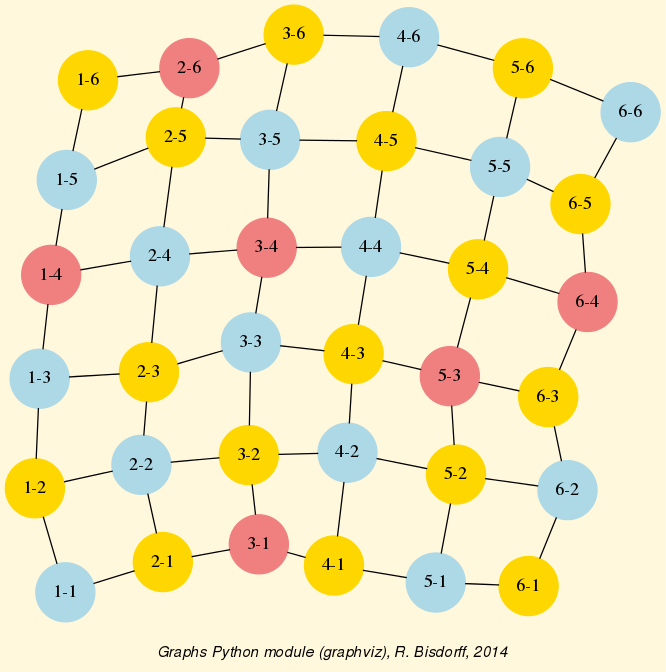
\includegraphics{grid-6-6-qcoloring.png}\hfill}
\end{quote}
\index{checkFeasibility() (graphs.Q\_Coloring method)}

\begin{fulllineitems}
\phantomsection\label{techDoc:graphs.Q_Coloring.checkFeasibility}\pysiglinewithargsret{\bfcode{checkFeasibility}}{\emph{Comments=True}, \emph{Debug=False}}{}
\end{fulllineitems}

\index{exportGraphViz() (graphs.Q\_Coloring method)}

\begin{fulllineitems}
\phantomsection\label{techDoc:graphs.Q_Coloring.exportGraphViz}\pysiglinewithargsret{\bfcode{exportGraphViz}}{\emph{fileName=None}, \emph{noSilent=True}, \emph{graphType='png'}, \emph{graphSize=`7}, \emph{7'}}{}
Exports GraphViz dot file  for q-coloring drawing filtering.
\begin{description}
\item[{Example:}] \leavevmode
\begin{Verbatim}[commandchars=\\\{\}]
\PYG{g+gp}{\PYGZgt{}\PYGZgt{}\PYGZgt{} }\PYG{n}{g} \PYG{o}{=} \PYG{n}{Graph}\PYG{p}{(}\PYG{n}{numberOfVertices}\PYG{o}{=}\PYG{l+m+mi}{10}\PYG{p}{,}\PYG{n}{edgeProbability}\PYG{o}{=}\PYG{l+m+mf}{0.4}\PYG{p}{)}
\PYG{g+gp}{\PYGZgt{}\PYGZgt{}\PYGZgt{} }\PYG{n}{g}\PYG{o}{.}\PYG{n}{showShort}\PYG{p}{(}\PYG{p}{)}
\PYG{g+go}{*\PYGZhy{}\PYGZhy{}\PYGZhy{}\PYGZhy{} short description of the graph \PYGZhy{}\PYGZhy{}\PYGZhy{}\PYGZhy{}*}
\PYG{g+go}{Name : \PYGZsq{}randomGraph\PYGZsq{}}
\PYG{g+go}{Vertices :  [\PYGZsq{}v1\PYGZsq{},\PYGZsq{}v10\PYGZsq{},\PYGZsq{}v2\PYGZsq{},\PYGZsq{}v3\PYGZsq{},\PYGZsq{}v4\PYGZsq{},\PYGZsq{}v5\PYGZsq{},\PYGZsq{}v6\PYGZsq{},\PYGZsq{}v7\PYGZsq{},\PYGZsq{}v8\PYGZsq{},\PYGZsq{}v9\PYGZsq{}]}
\PYG{g+go}{Valuation domain :  \PYGZob{}\PYGZsq{}max\PYGZsq{}: 1, \PYGZsq{}min\PYGZsq{}: \PYGZhy{}1, \PYGZsq{}med\PYGZsq{}: 0\PYGZcb{}}
\PYG{g+go}{Gamma function   : }
\PYG{g+go}{v1 \PYGZhy{}\PYGZgt{} [\PYGZsq{}v7\PYGZsq{}, \PYGZsq{}v2\PYGZsq{}, \PYGZsq{}v3\PYGZsq{}, \PYGZsq{}v5\PYGZsq{}]}
\PYG{g+go}{v10 \PYGZhy{}\PYGZgt{} [\PYGZsq{}v4\PYGZsq{}]}
\PYG{g+go}{v2 \PYGZhy{}\PYGZgt{} [\PYGZsq{}v1\PYGZsq{}, \PYGZsq{}v7\PYGZsq{}, \PYGZsq{}v8\PYGZsq{}]}
\PYG{g+go}{v3 \PYGZhy{}\PYGZgt{} [\PYGZsq{}v1\PYGZsq{}, \PYGZsq{}v7\PYGZsq{}, \PYGZsq{}v9\PYGZsq{}]}
\PYG{g+go}{v4 \PYGZhy{}\PYGZgt{} [\PYGZsq{}v5\PYGZsq{}, \PYGZsq{}v10\PYGZsq{}]}
\PYG{g+go}{v5 \PYGZhy{}\PYGZgt{} [\PYGZsq{}v6\PYGZsq{}, \PYGZsq{}v7\PYGZsq{}, \PYGZsq{}v1\PYGZsq{}, \PYGZsq{}v8\PYGZsq{}, \PYGZsq{}v4\PYGZsq{}]}
\PYG{g+go}{v6 \PYGZhy{}\PYGZgt{} [\PYGZsq{}v5\PYGZsq{}, \PYGZsq{}v8\PYGZsq{}]}
\PYG{g+go}{v7 \PYGZhy{}\PYGZgt{} [\PYGZsq{}v1\PYGZsq{}, \PYGZsq{}v5\PYGZsq{}, \PYGZsq{}v8\PYGZsq{}, \PYGZsq{}v2\PYGZsq{}, \PYGZsq{}v3\PYGZsq{}]}
\PYG{g+go}{v8 \PYGZhy{}\PYGZgt{} [\PYGZsq{}v6\PYGZsq{}, \PYGZsq{}v7\PYGZsq{}, \PYGZsq{}v2\PYGZsq{}, \PYGZsq{}v5\PYGZsq{}]}
\PYG{g+go}{v9 \PYGZhy{}\PYGZgt{} [\PYGZsq{}v3\PYGZsq{}]}
\PYG{g+gp}{\PYGZgt{}\PYGZgt{}\PYGZgt{} }\PYG{n}{qc} \PYG{o}{=} \PYG{n}{Q\PYGZus{}Coloring}\PYG{p}{(}\PYG{n}{g}\PYG{p}{,}\PYG{n}{nSim}\PYG{o}{=}\PYG{l+m+mi}{1000}\PYG{p}{)}
\PYG{g+go}{Running a Gibbs Sampler for 1000 step !}
\PYG{g+gp}{\PYGZgt{}\PYGZgt{}\PYGZgt{} }\PYG{n}{qc}\PYG{o}{.}\PYG{n}{checkFeasibility}\PYG{p}{(}\PYG{p}{)}
\PYG{g+go}{The q\PYGZhy{}coloring with 3 colors is feasible !!}
\PYG{g+gp}{\PYGZgt{}\PYGZgt{}\PYGZgt{} }\PYG{n}{qc}\PYG{o}{.}\PYG{n}{exportGraphViz}\PYG{p}{(}\PYG{p}{)}
\PYG{g+go}{*\PYGZhy{}\PYGZhy{}\PYGZhy{}\PYGZhy{} exporting a dot file for GraphViz tools \PYGZhy{}\PYGZhy{}\PYGZhy{}\PYGZhy{}\PYGZhy{}\PYGZhy{}\PYGZhy{}\PYGZhy{}\PYGZhy{}*}
\PYG{g+go}{Exporting to randomGraph\PYGZhy{}qcoloring.dot}
\PYG{g+go}{fdp \PYGZhy{}Tpng randomGraph\PYGZhy{}qcoloring.dot \PYGZhy{}o randomGraph\PYGZhy{}qcoloring.png}
\end{Verbatim}

\end{description}

{\hfill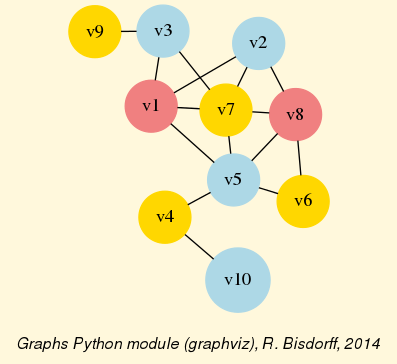
\includegraphics{randomGraph-qcoloring.png}\hfill}

\end{fulllineitems}

\index{generateFeasibleConfiguration() (graphs.Q\_Coloring method)}

\begin{fulllineitems}
\phantomsection\label{techDoc:graphs.Q_Coloring.generateFeasibleConfiguration}\pysiglinewithargsret{\bfcode{generateFeasibleConfiguration}}{\emph{Reset=True}, \emph{nSim=None}, \emph{Debug=False}}{}
\end{fulllineitems}

\index{showConfiguration() (graphs.Q\_Coloring method)}

\begin{fulllineitems}
\phantomsection\label{techDoc:graphs.Q_Coloring.showConfiguration}\pysiglinewithargsret{\bfcode{showConfiguration}}{}{}
\end{fulllineitems}


\end{fulllineitems}

\index{RandomGraph (class in graphs)}

\begin{fulllineitems}
\phantomsection\label{techDoc:graphs.RandomGraph}\pysiglinewithargsret{\strong{class }\code{graphs.}\bfcode{RandomGraph}}{\emph{order=5}, \emph{edgeProbability=0.4}}{}
Bases: {\hyperref[techDoc:graphs.Graph]{\code{graphs.Graph}}}

Random instances of the Graph class
\begin{description}
\item[{\emph{Parameters}:}] \leavevmode\begin{itemize}
\item {} 
order (positive integer)

\item {} 
edgeProbability (in {[}0,1{]})

\end{itemize}

\end{description}

\end{fulllineitems}

\index{RandomTree (class in graphs)}

\begin{fulllineitems}
\phantomsection\label{techDoc:graphs.RandomTree}\pysiglinewithargsret{\strong{class }\code{graphs.}\bfcode{RandomTree}}{\emph{order=None}, \emph{prueferCode=None}, \emph{myseed=None}, \emph{Debug=False}}{}
Bases: {\hyperref[techDoc:graphs.Graph]{\code{graphs.Graph}}}

Random instance of a tree generated from a random Prüfer code.

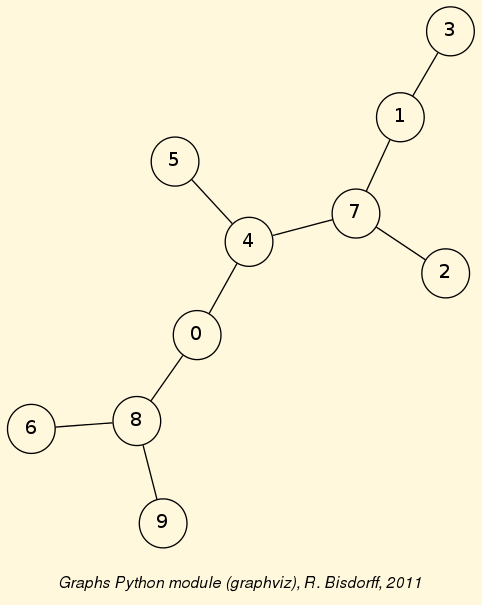
\includegraphics{randomTree.png}

\end{fulllineitems}

\index{TriangularGraph (class in graphs)}

\begin{fulllineitems}
\phantomsection\label{techDoc:graphs.TriangularGraph}\pysiglinewithargsret{\strong{class }\code{graphs.}\bfcode{TriangularGraph}}{\emph{n=5}, \emph{m=5}, \emph{valuationMin=-1}, \emph{valuationMax=1}}{}
Bases: {\hyperref[techDoc:graphs.Graph]{\code{graphs.Graph}}}

Specialization of the general Graph class for generating
temporary triangular graphs of dimension n times m.
\begin{description}
\item[{\emph{Parameters}:}] \leavevmode\begin{itemize}
\item {} 
n,m \textgreater{} 0

\item {} 
valuationDomain =\{`min':m, `max':M\}

\end{itemize}

\item[{Default instantiation (5 times 5 Trinagular Digraph):}] \leavevmode\begin{itemize}
\item {} 
n = 5,

\item {} 
m=5,

\item {} 
valuationDomain = \{`min':-1.0,'max':1.0\}.

\end{itemize}

\end{description}

Example of 5x5 GridGraph instance:

{\hfill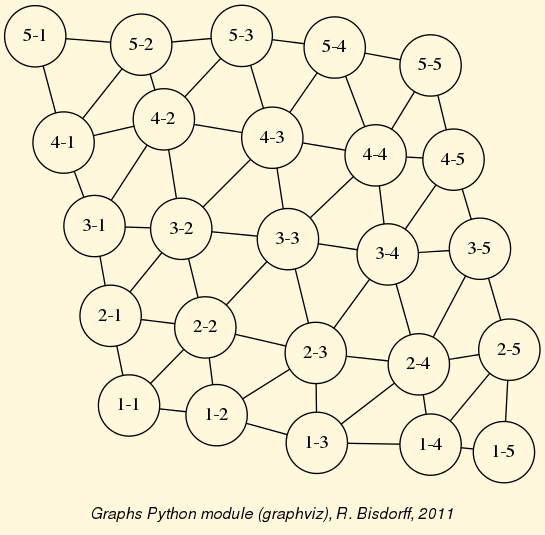
\includegraphics{triangular-5-5.png}\hfill}
\index{showShort() (graphs.TriangularGraph method)}

\begin{fulllineitems}
\phantomsection\label{techDoc:graphs.TriangularGraph.showShort}\pysiglinewithargsret{\bfcode{showShort}}{}{}
\end{fulllineitems}


\end{fulllineitems}


Back to the {\hyperref[techDoc:technical-label]{\emph{Introduction}}}


\subsection{perfTabs module}
\label{techDoc:module-perfTabs}\label{techDoc:perftabs-label}\label{techDoc:perftabs-module}\index{perfTabs (module)}\index{FullRandomPerformanceTableau (class in perfTabs)}

\begin{fulllineitems}
\phantomsection\label{techDoc:perfTabs.FullRandomPerformanceTableau}\pysiglinewithargsret{\strong{class }\code{perfTabs.}\bfcode{FullRandomPerformanceTableau}}{\emph{numberOfActions=None}, \emph{numberOfCriteria=None}, \emph{weightDistribution=None}, \emph{weightScale=None}, \emph{integerWeights=True}, \emph{commonScale=None}, \emph{commonThresholds=None}, \emph{commonMode=None}, \emph{valueDigits=2}, \emph{Debug=False}}{}
Bases: {\hyperref[techDoc:perfTabs.PerformanceTableau]{\code{perfTabs.PerformanceTableau}}}

Full automatic generation of random performance tableaux
\index{showAll() (perfTabs.FullRandomPerformanceTableau method)}

\begin{fulllineitems}
\phantomsection\label{techDoc:perfTabs.FullRandomPerformanceTableau.showAll}\pysiglinewithargsret{\bfcode{showAll}}{}{}
Show fonction for performance tableau of full random outranking digraph.

\end{fulllineitems}


\end{fulllineitems}

\index{NormalizedPerformanceTableau (class in perfTabs)}

\begin{fulllineitems}
\phantomsection\label{techDoc:perfTabs.NormalizedPerformanceTableau}\pysiglinewithargsret{\strong{class }\code{perfTabs.}\bfcode{NormalizedPerformanceTableau}}{\emph{argPerfTab=None}, \emph{lowValue=0}, \emph{highValue=100}, \emph{coalition=None}, \emph{Debug=False}}{}
Bases: {\hyperref[techDoc:perfTabs.PerformanceTableau]{\code{perfTabs.PerformanceTableau}}}

specialsation of the PerformanceTableau class for
constructing normalized, 0 - 100, valued PerformanceTableau
instances from a given argPerfTab instance.

\end{fulllineitems}

\index{OldXMCDAPerformanceTableau (class in perfTabs)}

\begin{fulllineitems}
\phantomsection\label{techDoc:perfTabs.OldXMCDAPerformanceTableau}\pysiglinewithargsret{\strong{class }\code{perfTabs.}\bfcode{OldXMCDAPerformanceTableau}}{\emph{fileName='temp'}}{}
Bases: {\hyperref[techDoc:perfTabs.PerformanceTableau]{\code{perfTabs.PerformanceTableau}}}

Specialization of the general PerformanceTableau class for reading
stored XMCDA formatted instances. Using the inbuilt module
xml.etree (for Python 2.5+).

Param: fileName (without the extension .xml or .xmcda).

\end{fulllineitems}

\index{PartialPerformanceTableau (class in perfTabs)}

\begin{fulllineitems}
\phantomsection\label{techDoc:perfTabs.PartialPerformanceTableau}\pysiglinewithargsret{\strong{class }\code{perfTabs.}\bfcode{PartialPerformanceTableau}}{\emph{inPerfTab}, \emph{actionsSubset=None}, \emph{criteriaSubset=None}}{}
Bases: {\hyperref[techDoc:perfTabs.PerformanceTableau]{\code{perfTabs.PerformanceTableau}}}

Constructor for partial performance tableaux.

\end{fulllineitems}

\index{PerformanceTableau (class in perfTabs)}

\begin{fulllineitems}
\phantomsection\label{techDoc:perfTabs.PerformanceTableau}\pysiglinewithargsret{\strong{class }\code{perfTabs.}\bfcode{PerformanceTableau}}{\emph{filePerfTab=None}, \emph{isEmpty=False}}{}
Bases: \code{builtins.object}

A general class for tacling MCDA performance tableaux.
\index{computeActionCriterionPerformanceDifferences() (perfTabs.PerformanceTableau method)}

\begin{fulllineitems}
\phantomsection\label{techDoc:perfTabs.PerformanceTableau.computeActionCriterionPerformanceDifferences}\pysiglinewithargsret{\bfcode{computeActionCriterionPerformanceDifferences}}{\emph{refAction}, \emph{refCriterion}, \emph{comments=False}, \emph{Debug=False}}{}
computes the performances differences observed between the reference action and the others on the given criterion

\end{fulllineitems}

\index{computeActionCriterionQuantile() (perfTabs.PerformanceTableau method)}

\begin{fulllineitems}
\phantomsection\label{techDoc:perfTabs.PerformanceTableau.computeActionCriterionQuantile}\pysiglinewithargsret{\bfcode{computeActionCriterionQuantile}}{\emph{action}, \emph{criterion}, \emph{Debug=False}}{}
renders the quantile of the performance of action on criterion

\end{fulllineitems}

\index{computeActionQuantile() (perfTabs.PerformanceTableau method)}

\begin{fulllineitems}
\phantomsection\label{techDoc:perfTabs.PerformanceTableau.computeActionQuantile}\pysiglinewithargsret{\bfcode{computeActionQuantile}}{\emph{action}, \emph{Debug=True}}{}
renders the overall performance quantile of action

\end{fulllineitems}

\index{computeCriterionPerformanceDifferences() (perfTabs.PerformanceTableau method)}

\begin{fulllineitems}
\phantomsection\label{techDoc:perfTabs.PerformanceTableau.computeCriterionPerformanceDifferences}\pysiglinewithargsret{\bfcode{computeCriterionPerformanceDifferences}}{\emph{c}, \emph{Comments=False}, \emph{Debug=False}}{}
Renders the ordered list of all observed performance differences on the given criterion.

\end{fulllineitems}

\index{computeDefaultDiscriminationThresholds() (perfTabs.PerformanceTableau method)}

\begin{fulllineitems}
\phantomsection\label{techDoc:perfTabs.PerformanceTableau.computeDefaultDiscriminationThresholds}\pysiglinewithargsret{\bfcode{computeDefaultDiscriminationThresholds}}{\emph{quantile=\{`weakVeto': 60}, \emph{`pref': 20}, \emph{`veto': 80}, \emph{`ind': 10\}}, \emph{Debug=False}, \emph{Comments=False}}{}
updates the discrimination thresholds with the percentiles
from the performance differences.
Parameters: quantile = \{`ind': 10, `pref': 20, `weakVeto': 60, `veto: 80\}.

\end{fulllineitems}

\index{computeMinMaxEvaluations() (perfTabs.PerformanceTableau method)}

\begin{fulllineitems}
\phantomsection\label{techDoc:perfTabs.PerformanceTableau.computeMinMaxEvaluations}\pysiglinewithargsret{\bfcode{computeMinMaxEvaluations}}{\emph{criteria=None}, \emph{actions=None}}{}
renders minimum and maximum performances on each criterion
in dictionary form: \{`g': \{`minimum': x, `maximum': x\}\}

\end{fulllineitems}

\index{computeNormalizedDiffEvaluations() (perfTabs.PerformanceTableau method)}

\begin{fulllineitems}
\phantomsection\label{techDoc:perfTabs.PerformanceTableau.computeNormalizedDiffEvaluations}\pysiglinewithargsret{\bfcode{computeNormalizedDiffEvaluations}}{\emph{lowValue=0.0}, \emph{highValue=100.0}, \emph{withOutput=False}, \emph{Debug=False}}{}
renders and csv stores (withOutput=True) the
list of normalized evaluation differences observed on the family of criteria
Is only adequate if all criteria have the same
evaluation scale. Therefore the performance tableau is normalized to 0.0-100.0 scales.

\end{fulllineitems}

\index{computePerformanceDifferences() (perfTabs.PerformanceTableau method)}

\begin{fulllineitems}
\phantomsection\label{techDoc:perfTabs.PerformanceTableau.computePerformanceDifferences}\pysiglinewithargsret{\bfcode{computePerformanceDifferences}}{\emph{Comments=False}, \emph{Debug=False}, \emph{NotPermanentDiffs=True}}{}
Adds to the criteria dictionary the ordered list of all observed performance differences.

\end{fulllineitems}

\index{computeQuantilePreorder() (perfTabs.PerformanceTableau method)}

\begin{fulllineitems}
\phantomsection\label{techDoc:perfTabs.PerformanceTableau.computeQuantilePreorder}\pysiglinewithargsret{\bfcode{computeQuantilePreorder}}{\emph{Comments=True}, \emph{Debug=False}}{}
computes the preorder of the actions obtained from decreasing majority quantiles. The quantiles are recomputed with a call to the self.computeQuantileSort() method.

\end{fulllineitems}

\index{computeQuantileSort() (perfTabs.PerformanceTableau method)}

\begin{fulllineitems}
\phantomsection\label{techDoc:perfTabs.PerformanceTableau.computeQuantileSort}\pysiglinewithargsret{\bfcode{computeQuantileSort}}{}{}
shows a sorting of the actions from decreasing majority quantiles

\end{fulllineitems}

\index{computeQuantiles() (perfTabs.PerformanceTableau method)}

\begin{fulllineitems}
\phantomsection\label{techDoc:perfTabs.PerformanceTableau.computeQuantiles}\pysiglinewithargsret{\bfcode{computeQuantiles}}{\emph{Debug=False}}{}
renders a quantiles matrix action x criterion with the performance quantile of action on criterion

\end{fulllineitems}

\index{computeThresholdPercentile() (perfTabs.PerformanceTableau method)}

\begin{fulllineitems}
\phantomsection\label{techDoc:perfTabs.PerformanceTableau.computeThresholdPercentile}\pysiglinewithargsret{\bfcode{computeThresholdPercentile}}{\emph{criterion}, \emph{threshold}, \emph{Debug=False}}{}
computes for a given criterion the quantile
of the performance differences of a given constant threshold.

\end{fulllineitems}

\index{computeVariableThresholdPercentile() (perfTabs.PerformanceTableau method)}

\begin{fulllineitems}
\phantomsection\label{techDoc:perfTabs.PerformanceTableau.computeVariableThresholdPercentile}\pysiglinewithargsret{\bfcode{computeVariableThresholdPercentile}}{\emph{criterion}, \emph{threshold}, \emph{Debug=False}}{}
computes for a given criterion the quantile
of the performance differences of a given threshold.

\end{fulllineitems}

\index{computeWeightPreorder() (perfTabs.PerformanceTableau method)}

\begin{fulllineitems}
\phantomsection\label{techDoc:perfTabs.PerformanceTableau.computeWeightPreorder}\pysiglinewithargsret{\bfcode{computeWeightPreorder}}{}{}
renders the weight preorder following from the given
criteria weights in a list of increasing equivalence
lists of criteria.

\end{fulllineitems}

\index{computeWeightedAveragePerformances() (perfTabs.PerformanceTableau method)}

\begin{fulllineitems}
\phantomsection\label{techDoc:perfTabs.PerformanceTableau.computeWeightedAveragePerformances}\pysiglinewithargsret{\bfcode{computeWeightedAveragePerformances}}{\emph{isNormalized=False}, \emph{lowValue=0.0}, \emph{highValue=100.0}, \emph{isListRanked=False}}{}
Compute normalized weighted average scores
Normalization transforms by default all the scores into a
common 0-100 scale. A lowValue and highValue parameter
can be provided for a specific normalisation.

\end{fulllineitems}

\index{csvAllQuantiles() (perfTabs.PerformanceTableau method)}

\begin{fulllineitems}
\phantomsection\label{techDoc:perfTabs.PerformanceTableau.csvAllQuantiles}\pysiglinewithargsret{\bfcode{csvAllQuantiles}}{\emph{fileName='quantiles'}}{}
save quantiles matrix criterionxaction in CSV format

\end{fulllineitems}

\index{hasOddWeightAlgebra() (perfTabs.PerformanceTableau method)}

\begin{fulllineitems}
\phantomsection\label{techDoc:perfTabs.PerformanceTableau.hasOddWeightAlgebra}\pysiglinewithargsret{\bfcode{hasOddWeightAlgebra}}{\emph{Debug=False}}{}
Verify if the given criteria{[}self{]}{[}'weight'{]} are odd or not.
Return a Boolen value.

\end{fulllineitems}

\index{htmlPerformanceTable() (perfTabs.PerformanceTableau method)}

\begin{fulllineitems}
\phantomsection\label{techDoc:perfTabs.PerformanceTableau.htmlPerformanceTable}\pysiglinewithargsret{\bfcode{htmlPerformanceTable}}{\emph{isSorted=True}, \emph{ndigits=2}}{}
Renders the performance table citerion x actions in html format.

\end{fulllineitems}

\index{normalizeEvaluations() (perfTabs.PerformanceTableau method)}

\begin{fulllineitems}
\phantomsection\label{techDoc:perfTabs.PerformanceTableau.normalizeEvaluations}\pysiglinewithargsret{\bfcode{normalizeEvaluations}}{\emph{lowValue=0.0}, \emph{highValue=100.0}, \emph{Debug=False}}{}
recode the evaluations between lowValue and highValue on all criteria

\end{fulllineitems}

\index{save() (perfTabs.PerformanceTableau method)}

\begin{fulllineitems}
\phantomsection\label{techDoc:perfTabs.PerformanceTableau.save}\pysiglinewithargsret{\bfcode{save}}{\emph{fileName='tempperftab'}, \emph{isDecimal=True}, \emph{valueDigits=2}}{}
Persistant storage of Performance Tableaux.

\end{fulllineitems}

\index{saveXMCDA() (perfTabs.PerformanceTableau method)}

\begin{fulllineitems}
\phantomsection\label{techDoc:perfTabs.PerformanceTableau.saveXMCDA}\pysiglinewithargsret{\bfcode{saveXMCDA}}{\emph{fileName='temp'}, \emph{category='New XMCDA Rubis format'}, \emph{user='digraphs Module (RB)'}, \emph{version='saved from Python session'}, \emph{variant='Rubis'}, \emph{valuationType='standard'}, \emph{servingD3=True}}{}
save performance tableau object self in XMCDA format.

\end{fulllineitems}

\index{saveXMCDA2() (perfTabs.PerformanceTableau method)}

\begin{fulllineitems}
\phantomsection\label{techDoc:perfTabs.PerformanceTableau.saveXMCDA2}\pysiglinewithargsret{\bfcode{saveXMCDA2}}{\emph{fileName='temp'}, \emph{category='XMCDA 2.0 format'}, \emph{user='digraphs Module (RB)'}, \emph{version='saved from Python session'}, \emph{title='Performance Tableau in XMCDA-2.0 format.'}, \emph{variant='Rubis'}, \emph{valuationType='bipolar'}, \emph{servingD3=True}, \emph{isStringIO=False}, \emph{stringNA='NA'}, \emph{comment='produced by saveXMCDA2()'}, \emph{hasVeto=True}}{}
save performance tableau object self in XMCDA 2.0 format.

\end{fulllineitems}

\index{saveXMCDA2String() (perfTabs.PerformanceTableau method)}

\begin{fulllineitems}
\phantomsection\label{techDoc:perfTabs.PerformanceTableau.saveXMCDA2String}\pysiglinewithargsret{\bfcode{saveXMCDA2String}}{\emph{fileName='temp'}, \emph{category='XMCDA 2.0 format'}, \emph{user='digraphs Module (RB)'}, \emph{version='saved from Python session'}, \emph{title='Performance Tableau in XMCDA-2.0 format.'}, \emph{variant='Rubis'}, \emph{valuationType='bipolar'}, \emph{servingD3=True}, \emph{comment='produced by stringIO()'}, \emph{stringNA='NA'}}{}
save performance tableau object self in XMCDA 2.0 format.
!!! obsolete: replaced by the isStringIO in the saveXMCDA2 method !!!

\end{fulllineitems}

\index{saveXML() (perfTabs.PerformanceTableau method)}

\begin{fulllineitems}
\phantomsection\label{techDoc:perfTabs.PerformanceTableau.saveXML}\pysiglinewithargsret{\bfcode{saveXML}}{\emph{name='temp'}, \emph{category='standard'}, \emph{subcategory='standard'}, \emph{author='digraphs Module (RB)'}, \emph{reference='saved from Python'}}{}
save temporary performance tableau self in XML format.

\end{fulllineitems}

\index{saveXMLRubis() (perfTabs.PerformanceTableau method)}

\begin{fulllineitems}
\phantomsection\label{techDoc:perfTabs.PerformanceTableau.saveXMLRubis}\pysiglinewithargsret{\bfcode{saveXMLRubis}}{\emph{name='temp'}, \emph{category='Rubis'}, \emph{subcategory='new D2 version'}, \emph{author='digraphs Module (RB)'}, \emph{reference='saved from Python'}}{}
save temporary performance tableau self in XML Rubis format.

\end{fulllineitems}

\index{showAll() (perfTabs.PerformanceTableau method)}

\begin{fulllineitems}
\phantomsection\label{techDoc:perfTabs.PerformanceTableau.showAll}\pysiglinewithargsret{\bfcode{showAll}}{}{}
Show fonction for performance tableau

\end{fulllineitems}

\index{showAllQuantiles() (perfTabs.PerformanceTableau method)}

\begin{fulllineitems}
\phantomsection\label{techDoc:perfTabs.PerformanceTableau.showAllQuantiles}\pysiglinewithargsret{\bfcode{showAllQuantiles}}{}{}
renders a html string showing the table of
the quantiles matrix action x criterion

\end{fulllineitems}

\index{showCriteria() (perfTabs.PerformanceTableau method)}

\begin{fulllineitems}
\phantomsection\label{techDoc:perfTabs.PerformanceTableau.showCriteria}\pysiglinewithargsret{\bfcode{showCriteria}}{\emph{IntegerWeights=False}, \emph{Debug=False}}{}
print Criteria with thresholds and weights.

\end{fulllineitems}

\index{showEvaluationStatistics() (perfTabs.PerformanceTableau method)}

\begin{fulllineitems}
\phantomsection\label{techDoc:perfTabs.PerformanceTableau.showEvaluationStatistics}\pysiglinewithargsret{\bfcode{showEvaluationStatistics}}{}{}
renders the variance and standard deviation of
the values observed in the performance Tableau.

\end{fulllineitems}

\index{showHTMLPerformanceTableau() (perfTabs.PerformanceTableau method)}

\begin{fulllineitems}
\phantomsection\label{techDoc:perfTabs.PerformanceTableau.showHTMLPerformanceTableau}\pysiglinewithargsret{\bfcode{showHTMLPerformanceTableau}}{\emph{isSorted=True}, \emph{ndigits=2}}{}
shows the html version of the performance tableau in a browser window.

\end{fulllineitems}

\index{showPerformanceTableau() (perfTabs.PerformanceTableau method)}

\begin{fulllineitems}
\phantomsection\label{techDoc:perfTabs.PerformanceTableau.showPerformanceTableau}\pysiglinewithargsret{\bfcode{showPerformanceTableau}}{\emph{sorted=True}, \emph{ndigits=2}}{}
Print the performance Tableau.

\end{fulllineitems}

\index{showQuantileSort() (perfTabs.PerformanceTableau method)}

\begin{fulllineitems}
\phantomsection\label{techDoc:perfTabs.PerformanceTableau.showQuantileSort}\pysiglinewithargsret{\bfcode{showQuantileSort}}{\emph{Debug=False}}{}
Wrapper of computeQuantilePreorder() for the obsolete showQuantileSort() method.

\end{fulllineitems}

\index{showStatistics() (perfTabs.PerformanceTableau method)}

\begin{fulllineitems}
\phantomsection\label{techDoc:perfTabs.PerformanceTableau.showStatistics}\pysiglinewithargsret{\bfcode{showStatistics}}{}{}
show statistics concerning the evaluation distributions
on each criteria.

\end{fulllineitems}


\end{fulllineitems}

\index{RandomCBPerformanceTableau (class in perfTabs)}

\begin{fulllineitems}
\phantomsection\label{techDoc:perfTabs.RandomCBPerformanceTableau}\pysiglinewithargsret{\strong{class }\code{perfTabs.}\bfcode{RandomCBPerformanceTableau}}{\emph{numberOfActions=None}, \emph{numberOfCriteria=None}, \emph{weightDistribution=None}, \emph{weightScale=None}, \emph{integerWeights=True}, \emph{commonScale=None}, \emph{commonThresholds=None}, \emph{commonPercentiles=None}, \emph{commonMode=None}, \emph{valueDigits=2}, \emph{Debug=False}, \emph{Comments=False}}{}
Bases: {\hyperref[techDoc:perfTabs.PerformanceTableau]{\code{perfTabs.PerformanceTableau}}}

Full automatic generation of random
Cost versus Benefit oriented performance tableaux.
\begin{description}
\item[{Parameters:}] \leavevmode
\begin{DUlineblock}{0em}
\item[] If numberOfActions == None, a uniform random number between 10 and 31 of cheap, neutral or advantageous actions (equal 1/3 probability each type) actions is instantiated
\item[] If numberOfCriteria == None, a uniform random number between 5 and 21 of cost or benefit criteria (1/3 respectively 2/3 probability) is instantiated
\item[] weightDistribution := \{`equiobjectives'\textbar{}'fixed'\textbar{}'random'\textbar{}'equisignificant' (default = `equisignificant')\}
\item[] default weightScale for `random' weightDistribution is 1 - numberOfCriteria
\item[] commonScale parameter is obsolete. The scale of cost criteria is cardinal or ordinal (0-10) with proabailities 1/4 respectively 3/4, whereas the scale of benefit criteria is ordinal or cardinal with probabilities 2/3, respectively 1/3.
\item[] All cardinal criteria are evaluated with decimals between 0.0 and 100.0 wheras all ordinal criteria are evaluated with integers between 0 and 10.
\item[] commonThresholds is obsolete. Preference discrimination is specified as percentiles of concerned performance differences (see below).
\item[] CommonPercentiles = \{`ind':5, `pref':10, {[}'weakveto':90,{]} `veto':95\} are expressed in percents (reversed for vetoes) and only concern cardinal criteria.
\end{DUlineblock}

\end{description}

\begin{notice}{warning}{Warning:}
Minimal number of decision actions required is 3 !
\end{notice}

\end{fulllineitems}

\index{RandomCoalitionsPerformanceTableau (class in perfTabs)}

\begin{fulllineitems}
\phantomsection\label{techDoc:perfTabs.RandomCoalitionsPerformanceTableau}\pysiglinewithargsret{\strong{class }\code{perfTabs.}\bfcode{RandomCoalitionsPerformanceTableau}}{\emph{numberOfActions=None}, \emph{numberOfCriteria=None}, \emph{weightDistribution=None}, \emph{weightScale=None}, \emph{integerWeights=True}, \emph{commonScale=None}, \emph{commonThresholds=None}, \emph{commonMode=None}, \emph{valueDigits=2}, \emph{Coalitions=True}, \emph{VariableGenerators=True}, \emph{OrdinalScales=False}, \emph{Debug=False}, \emph{RandomCoalitions=False}, \emph{vetoProbability=None}, \emph{Electre3=True}}{}
Bases: {\hyperref[techDoc:perfTabs.PerformanceTableau]{\code{perfTabs.PerformanceTableau}}}

Full automatic generation of performance tableaux with random coalitions of criteria
\begin{description}
\item[{Parameters:}] \leavevmode
\begin{DUlineblock}{0em}
\item[] numberOf Actions := 20 (default)
\item[] number of Criteria := 13 (default)
\item[] weightDistribution := `equisignificant' (default with all weights = 1.0), `random', `fixed' (default w\_1 = numberOfCriteria-1, w\_\{i!=1\} = 1
\item[] weightScale := {[}1,numerOfCriteria{[} (random default), {[}w\_1, w\_\{i!=1{]} (fixed)
\item[] integerWeights := True (default) / False
\item[] commonScale := (0.0, 100.0) (default)
\item[] commonThresholds := {[}(1.0,0.0),(2.001,0.0),(8.001,0.0){]} if OrdinalSacles, {[}(0.10001*span,0),(0.20001*span,0.0),(0.80001*span,0.0){]} with span = commonScale{[}1{]} - commonScale{[}0{]}.
\item[] commonMode := {[}'triangular',50.0,0.50{]} (default), {[}'uniform',None,None{]}, {[}'beta', None,None{]} (three alpha, beta combinations (5.8661,2.62203) chosen by default for high(`+'), medium (`\textasciitilde{}') and low (`-`) evaluations.
\item[] valueDigits := 2 (default, for cardinal scales only)
\item[] Coalitions := True (default)/False, three coalitions if True
\item[] VariableGenerators := True (default) / False, variable high(`+'), medium (`\textasciitilde{}') or low (`-`) law generated evaluations.
\item[] OrdinalScales := True / False (default)
\item[] Debug := True / False (default)
\item[] RandomCoalitions = True / False (default) zero or more than three coalitions if Coalitions == False.
\item[] vetoProbability := x in {]}0.0-1.0{[} / None (default), probability that a cardinal criterion shows a veto preference discrimination threshold.
\item[] Electre3 := True (default) / False, no weakveto if True (obsolete)
\end{DUlineblock}

\end{description}

\end{fulllineitems}

\index{RandomPerformanceTableau (class in perfTabs)}

\begin{fulllineitems}
\phantomsection\label{techDoc:perfTabs.RandomPerformanceTableau}\pysiglinewithargsret{\strong{class }\code{perfTabs.}\bfcode{RandomPerformanceTableau}}{\emph{numberOfActions=None, numberOfCriteria=None, weightDistribution=None, weightScale=None, integerWeights=True, commonScale={[}0.0, 100.0{]}, commonThresholds={[}(10.0, 0.0), (20.0, 0.0), (80.0, 0.0){]}, commonMode=None, valueDigits=2, Debug=False}}{}
Bases: {\hyperref[techDoc:perfTabs.PerformanceTableau]{\code{perfTabs.PerformanceTableau}}}

Specialization of the PerformanceTableau class for generating a temporary
random performance tableau.
\begin{description}
\item[{Parameters:}] \leavevmode
\begin{DUlineblock}{0em}
\item[] actions := nbr of actions,
\item[] criteria := number criteria,
\item[] scale := {[}Min,Max{]},
\item[] thresholds := {[}q,p,v{]},
\item[] mode = {[}
\textbar{} (`uniform',None,None)
\textbar{} (`normal',mu,sigma)
\textbar{} (`triangular',mode,None)
\textbar{} (`beta',mode,(alpha,beta){]},
\item[] weightDistribution := equivalent\textbar{}random\textbar{}fixed
\end{DUlineblock}

\item[{Code example::}] \leavevmode
\begin{Verbatim}[commandchars=\\\{\}]
\PYG{g+gp}{\PYGZgt{}\PYGZgt{}\PYGZgt{} }\PYG{k+kn}{from} \PYG{n+nn}{perfTabs} \PYG{k+kn}{import} \PYG{n}{RandomCBPerformanceTableau}
\PYG{g+gp}{\PYGZgt{}\PYGZgt{}\PYGZgt{} }\PYG{n}{t} \PYG{o}{=} \PYG{n}{RandomCBPerformanceTableau}\PYG{p}{(}\PYG{n}{numberOfActions}\PYG{o}{=}\PYG{l+m+mi}{3}\PYG{p}{,}\PYG{n}{numberOfCriteria}\PYG{o}{=}\PYG{l+m+mi}{1}\PYG{p}{)}
\PYG{g+gp}{\PYGZgt{}\PYGZgt{}\PYGZgt{} }\PYG{n}{t}\PYG{o}{.}\PYG{n}{actions}
\PYG{g+go}{    \PYGZob{}\PYGZsq{}a02\PYGZsq{}: \PYGZob{}\PYGZsq{}comment\PYGZsq{}: \PYGZsq{}RandomCBPerformanceTableau() generated.\PYGZsq{}, \PYGZsq{}type\PYGZsq{}: \PYGZsq{}advantageous\PYGZsq{}, \PYGZsq{}name\PYGZsq{}: \PYGZsq{}random advantageous decision action\PYGZsq{}\PYGZcb{},}
\PYG{g+go}{    \PYGZsq{}a03\PYGZsq{}: \PYGZob{}\PYGZsq{}comment\PYGZsq{}: \PYGZsq{}RandomCBPerformanceTableau() generated.\PYGZsq{}, \PYGZsq{}type\PYGZsq{}: \PYGZsq{}advantageous\PYGZsq{}, \PYGZsq{}name\PYGZsq{}: \PYGZsq{}random advantageous decision action\PYGZsq{}\PYGZcb{},}
\PYG{g+go}{    \PYGZsq{}a01\PYGZsq{}: \PYGZob{}\PYGZsq{}comment\PYGZsq{}: \PYGZsq{}RandomCBPerformanceTableau() generated.\PYGZsq{}, \PYGZsq{}type\PYGZsq{}: \PYGZsq{}neutral\PYGZsq{}, \PYGZsq{}name\PYGZsq{}: \PYGZsq{}random neutral decision action\PYGZsq{}\PYGZcb{}\PYGZcb{}}
\PYG{g+gp}{\PYGZgt{}\PYGZgt{}\PYGZgt{} }\PYG{n}{t}\PYG{o}{.}\PYG{n}{criteria}
\PYG{g+go}{    \PYGZob{}\PYGZsq{}g01\PYGZsq{}: \PYGZob{}\PYGZsq{}comment\PYGZsq{}: \PYGZsq{}Evaluation generator: triangular law with variable mode (m) and probability repartition (p = 0.5). Cheap actions: m = 30\PYGZpc{}; neutral actions: m = 50\PYGZpc{}; advantageous actions: m = 70\PYGZpc{}.\PYGZsq{},}
\PYG{g+go}{    \PYGZsq{}performanceDifferences\PYGZsq{}: [Decimal(\PYGZsq{}21.84\PYGZsq{}), Decimal(\PYGZsq{}25.49\PYGZsq{}), Decimal(\PYGZsq{}47.33\PYGZsq{})],}
\PYG{g+go}{    \PYGZsq{}scale\PYGZsq{}: (0.0, 100.0),}
\PYG{g+go}{    \PYGZsq{}minimalPerformanceDifference\PYGZsq{}: Decimal(\PYGZsq{}21.84\PYGZsq{}),}
\PYG{g+go}{    \PYGZsq{}preferenceDirection\PYGZsq{}: \PYGZsq{}max\PYGZsq{},}
\PYG{g+go}{    \PYGZsq{}weight\PYGZsq{}: Decimal(\PYGZsq{}1\PYGZsq{}),}
\PYG{g+go}{    \PYGZsq{}randomMode\PYGZsq{}: [\PYGZsq{}triangular\PYGZsq{}, 50.0, 0.5],}
\PYG{g+go}{                   \PYGZsq{}name\PYGZsq{}: \PYGZsq{}random cardinal benefit criterion\PYGZsq{},}
\PYG{g+go}{                   \PYGZsq{}maximalPerformanceDifference\PYGZsq{}: Decimal(\PYGZsq{}47.33\PYGZsq{}),}
\PYG{g+go}{                   \PYGZsq{}thresholds\PYGZsq{}: \PYGZob{}\PYGZsq{}ind\PYGZsq{}: (Decimal(\PYGZsq{}22.205\PYGZsq{}), Decimal(\PYGZsq{}0.0\PYGZsq{})),}
\PYG{g+go}{                                  \PYGZsq{}veto\PYGZsq{}: (Decimal(\PYGZsq{}45.146\PYGZsq{}), Decimal(\PYGZsq{}0.0\PYGZsq{})),}
\PYG{g+go}{                                  \PYGZsq{}pref\PYGZsq{}: (Decimal(\PYGZsq{}22.570\PYGZsq{}), Decimal(\PYGZsq{}0.0\PYGZsq{}))\PYGZcb{},}
\PYG{g+go}{    \PYGZsq{}scaleType\PYGZsq{}: \PYGZsq{}cardinal\PYGZsq{}\PYGZcb{}}
\PYG{g+go}{    \PYGZcb{}}
\end{Verbatim}

\begin{Verbatim}[commandchars=\\\{\}]
\PYG{g+gp}{\PYGZgt{}\PYGZgt{}\PYGZgt{} }\PYG{n}{t}\PYG{o}{.}\PYG{n}{evaluation}
\PYG{g+go}{    \PYGZob{}\PYGZsq{}g01\PYGZsq{}: \PYGZob{}\PYGZsq{}a02\PYGZsq{}: Decimal(\PYGZsq{}94.22\PYGZsq{}),}
\PYG{g+go}{             \PYGZsq{}a03\PYGZsq{}: Decimal(\PYGZsq{}72.38\PYGZsq{}),}
\PYG{g+go}{             \PYGZsq{}a01\PYGZsq{}: Decimal(\PYGZsq{}46.89\PYGZsq{})}
\PYG{g+go}{            \PYGZcb{}}
\PYG{g+go}{    \PYGZcb{}}
\end{Verbatim}

\end{description}

\end{fulllineitems}

\index{RandomRankPerformanceTableau (class in perfTabs)}

\begin{fulllineitems}
\phantomsection\label{techDoc:perfTabs.RandomRankPerformanceTableau}\pysiglinewithargsret{\strong{class }\code{perfTabs.}\bfcode{RandomRankPerformanceTableau}}{\emph{numberOfActions=None}, \emph{numberOfCriteria=None}, \emph{weightDistribution=None}, \emph{weightScale=None}, \emph{commonThresholds=None}, \emph{integerWeights=True}, \emph{Debug=False}}{}
Bases: {\hyperref[techDoc:perfTabs.PerformanceTableau]{\code{perfTabs.PerformanceTableau}}}

Specialization of the PerformanceTableau class for generating a temporary
random performance tableau.

\end{fulllineitems}

\index{RandomS3PerformanceTableau (class in perfTabs)}

\begin{fulllineitems}
\phantomsection\label{techDoc:perfTabs.RandomS3PerformanceTableau}\pysiglinewithargsret{\strong{class }\code{perfTabs.}\bfcode{RandomS3PerformanceTableau}}{\emph{numberOfActions=None}, \emph{numberOfCriteria=None}, \emph{weightDistribution=None}, \emph{weightScale=None}, \emph{integerWeights=True}, \emph{commonScale=None}, \emph{commonThresholds=None}, \emph{commonMode=None}, \emph{valueDigits=2}, \emph{Coalitions=True}, \emph{VariableGenerators=True}, \emph{OrdinalScales=False}, \emph{Debug=False}, \emph{RandomCoalitions=False}, \emph{vetoProbability=None}, \emph{Electre3=True}}{}
Bases: {\hyperref[techDoc:perfTabs.RandomCoalitionsPerformanceTableau]{\code{perfTabs.RandomCoalitionsPerformanceTableau}}}

Obsolete dummy class for backports.

\end{fulllineitems}

\index{XMCDA2PerformanceTableau (class in perfTabs)}

\begin{fulllineitems}
\phantomsection\label{techDoc:perfTabs.XMCDA2PerformanceTableau}\pysiglinewithargsret{\strong{class }\code{perfTabs.}\bfcode{XMCDA2PerformanceTableau}}{\emph{fileName='temp'}, \emph{HasSeparatedWeights=False}, \emph{HasSeparatedThresholds=False}, \emph{stringInput=None}}{}
Bases: {\hyperref[techDoc:perfTabs.PerformanceTableau]{\code{perfTabs.PerformanceTableau}}}

Specialization of the general PerformanceTableau class for reading
stored XMCDA 2.0 formatted instances with exact decimal numbers.
Using the inbuilt module xml.etree (for Python 2.5+).

Parameters:
\begin{quote}

fileName (without the extension .xml or .xmcda)
HasSeparatedWeights - XMCDA 2.0.0 encoding (default = False)
HasSeparatedThresholds - XMCDA 2.0.0 encoding (default = False)
stringInput (default = None)
\end{quote}

\end{fulllineitems}

\index{XMCDAPerformanceTableau (class in perfTabs)}

\begin{fulllineitems}
\phantomsection\label{techDoc:perfTabs.XMCDAPerformanceTableau}\pysiglinewithargsret{\strong{class }\code{perfTabs.}\bfcode{XMCDAPerformanceTableau}}{\emph{fileName='temp'}}{}
Bases: {\hyperref[techDoc:perfTabs.PerformanceTableau]{\code{perfTabs.PerformanceTableau}}}

Specialization of the general PerformanceTableau class for reading
stored XMCDA formatted instances with exact decimal numbers.
Using the inbuilt module
xml.etree (for Python 2.5+).

Param: fileName (without the extension .xml or .xmcda).

\end{fulllineitems}

\index{XMLPerformanceTableau (class in perfTabs)}

\begin{fulllineitems}
\phantomsection\label{techDoc:perfTabs.XMLPerformanceTableau}\pysiglinewithargsret{\strong{class }\code{perfTabs.}\bfcode{XMLPerformanceTableau}}{\emph{fileName='testperftabXML'}}{}
Bases: {\hyperref[techDoc:perfTabs.PerformanceTableau]{\code{perfTabs.PerformanceTableau}}}

Specialization of the general PerformanceTableau class for reading
stored XML formatted instances.

\end{fulllineitems}

\index{XMLRubisPerformanceTableau (class in perfTabs)}

\begin{fulllineitems}
\phantomsection\label{techDoc:perfTabs.XMLRubisPerformanceTableau}\pysiglinewithargsret{\strong{class }\code{perfTabs.}\bfcode{XMLRubisPerformanceTableau}}{\emph{fileName='rubisPerformanceTableau'}}{}
Bases: {\hyperref[techDoc:perfTabs.PerformanceTableau]{\code{perfTabs.PerformanceTableau}}}

Specialization of the general PerformanceTableau class for reading
stored XML formatted instances. Using the inbuilt module
xml.etree (for Python 2.5+).

Param: fileName (without the extension .xml).
\index{stripsplit() (perfTabs.XMLRubisPerformanceTableau method)}

\begin{fulllineitems}
\phantomsection\label{techDoc:perfTabs.XMLRubisPerformanceTableau.stripsplit}\pysiglinewithargsret{\bfcode{stripsplit}}{\emph{th}}{}
extract thresholds new Python 3 compatible version

\end{fulllineitems}


\end{fulllineitems}


Back to the {\hyperref[techDoc:technical-label]{\emph{Introduction}}}


\subsection{outrankingDigraphs module}
\label{techDoc:outrankingdigraphs-label}\label{techDoc:module-outrankingDigraphs}\label{techDoc:outrankingdigraphs-module}\index{outrankingDigraphs (module)}\index{BipolarIntegerOutrankingDigraph (class in outrankingDigraphs)}

\begin{fulllineitems}
\phantomsection\label{techDoc:outrankingDigraphs.BipolarIntegerOutrankingDigraph}\pysiglinewithargsret{\strong{class }\code{outrankingDigraphs.}\bfcode{BipolarIntegerOutrankingDigraph}}{\emph{argPerfTab=None}, \emph{coalition=None}, \emph{hasBipolarVeto=True}, \emph{hasSymmetricThresholds=True}}{}
Bases: {\hyperref[techDoc:outrankingDigraphs.BipolarOutrankingDigraph]{\code{outrankingDigraphs.BipolarOutrankingDigraph}}}, {\hyperref[techDoc:perfTabs.PerformanceTableau]{\code{perfTabs.PerformanceTableau}}}
\begin{description}
\item[{Parameters:}] \leavevmode
\begin{DUlineblock}{0em}
\item[] performanceTableau (fileName of valid py code)
\item[] optional, coalition (sublist of criteria)
\end{DUlineblock}

\end{description}

Specialization of the standard OutrankingDigraph class for generating
bipolar integer-valued outranking digraphs.
\index{savePy2Gprolog() (outrankingDigraphs.BipolarIntegerOutrankingDigraph method)}

\begin{fulllineitems}
\phantomsection\label{techDoc:outrankingDigraphs.BipolarIntegerOutrankingDigraph.savePy2Gprolog}\pysiglinewithargsret{\bfcode{savePy2Gprolog}}{\emph{name='temp'}}{}
save digraph in gprolog version

\end{fulllineitems}

\index{showRelation() (outrankingDigraphs.BipolarIntegerOutrankingDigraph method)}

\begin{fulllineitems}
\phantomsection\label{techDoc:outrankingDigraphs.BipolarIntegerOutrankingDigraph.showRelation}\pysiglinewithargsret{\bfcode{showRelation}}{}{}
prints the relation valuation in \#\#.\#\# format.

\end{fulllineitems}


\end{fulllineitems}

\index{BipolarOutrankingDigraph (class in outrankingDigraphs)}

\begin{fulllineitems}
\phantomsection\label{techDoc:outrankingDigraphs.BipolarOutrankingDigraph}\pysiglinewithargsret{\strong{class }\code{outrankingDigraphs.}\bfcode{BipolarOutrankingDigraph}}{\emph{argPerfTab=None}, \emph{coalition=None}, \emph{hasNoVeto=False}, \emph{hasBipolarVeto=True}, \emph{Normalized=False}}{}
Bases: {\hyperref[techDoc:outrankingDigraphs.OutrankingDigraph]{\code{outrankingDigraphs.OutrankingDigraph}}}, {\hyperref[techDoc:perfTabs.PerformanceTableau]{\code{perfTabs.PerformanceTableau}}}

Specialization of the standard OutrankingDigraph class for generating
new bipolar ordinal-valued outranking digraphs.
\begin{description}
\item[{Parameters:}] \leavevmode
\begin{DUlineblock}{0em}
\item[] performanceTableau (fileName of valid py code)
\item[] optional, coalition (sublist of criteria)
\end{DUlineblock}

\end{description}
\index{computeCriterionRelation() (outrankingDigraphs.BipolarOutrankingDigraph method)}

\begin{fulllineitems}
\phantomsection\label{techDoc:outrankingDigraphs.BipolarOutrankingDigraph.computeCriterionRelation}\pysiglinewithargsret{\bfcode{computeCriterionRelation}}{\emph{c}, \emph{a}, \emph{b}, \emph{hasSymmetricThresholds=True}}{}
Compute the outranking characteristic for actions x and y
on criterion c.

\end{fulllineitems}

\index{computeSingleCriteriaNetflows() (outrankingDigraphs.BipolarOutrankingDigraph method)}

\begin{fulllineitems}
\phantomsection\label{techDoc:outrankingDigraphs.BipolarOutrankingDigraph.computeSingleCriteriaNetflows}\pysiglinewithargsret{\bfcode{computeSingleCriteriaNetflows}}{}{}
renders the Promethee single criteria netflows matrix M

\end{fulllineitems}

\index{criterionCharacteristicFunction() (outrankingDigraphs.BipolarOutrankingDigraph method)}

\begin{fulllineitems}
\phantomsection\label{techDoc:outrankingDigraphs.BipolarOutrankingDigraph.criterionCharacteristicFunction}\pysiglinewithargsret{\bfcode{criterionCharacteristicFunction}}{\emph{c}, \emph{a}, \emph{b}, \emph{hasSymmetricThresholds=True}}{}
Renders the characteristic value of the comparison of a and b on criterion c.

\end{fulllineitems}

\index{saveSingleCriterionNetflows() (outrankingDigraphs.BipolarOutrankingDigraph method)}

\begin{fulllineitems}
\phantomsection\label{techDoc:outrankingDigraphs.BipolarOutrankingDigraph.saveSingleCriterionNetflows}\pysiglinewithargsret{\bfcode{saveSingleCriterionNetflows}}{\emph{fileName='tempnetflows.prn'}, \emph{delimiter=' `}, \emph{Comments=True}}{}
Delimited save of single criteria netflows matrix

\end{fulllineitems}


\end{fulllineitems}

\index{BipolarPreferenceDigraph (class in outrankingDigraphs)}

\begin{fulllineitems}
\phantomsection\label{techDoc:outrankingDigraphs.BipolarPreferenceDigraph}\pysiglinewithargsret{\strong{class }\code{outrankingDigraphs.}\bfcode{BipolarPreferenceDigraph}}{\emph{argPerfTab=None}, \emph{coalition=None}}{}
Bases: {\hyperref[techDoc:outrankingDigraphs.BipolarOutrankingDigraph]{\code{outrankingDigraphs.BipolarOutrankingDigraph}}}, {\hyperref[techDoc:perfTabs.PerformanceTableau]{\code{perfTabs.PerformanceTableau}}}
\begin{description}
\item[{Parameters:}] \leavevmode
\begin{DUlineblock}{0em}
\item[] performanceTableau (fileName of valid py code)
\item[] optional, coalition (sublist of criteria)
\end{DUlineblock}

\end{description}

Specialization of the standard BipolarOutrankingDigraph class for generating
new bipolar ordinal-valued outranking digraphs.
\index{computeSingleCriteriaNetflows() (outrankingDigraphs.BipolarPreferenceDigraph method)}

\begin{fulllineitems}
\phantomsection\label{techDoc:outrankingDigraphs.BipolarPreferenceDigraph.computeSingleCriteriaNetflows}\pysiglinewithargsret{\bfcode{computeSingleCriteriaNetflows}}{}{}
renders the Promethee single criteria netflows matrix M

\end{fulllineitems}

\index{criterionCharacteristicFunction() (outrankingDigraphs.BipolarPreferenceDigraph method)}

\begin{fulllineitems}
\phantomsection\label{techDoc:outrankingDigraphs.BipolarPreferenceDigraph.criterionCharacteristicFunction}\pysiglinewithargsret{\bfcode{criterionCharacteristicFunction}}{\emph{c}, \emph{a}, \emph{b}, \emph{hasSymmetricThresholds=True}}{}
Renders the characteristic value of the comparison of a and b on criterion c.

\end{fulllineitems}

\index{saveSingleCriterionNetflows() (outrankingDigraphs.BipolarPreferenceDigraph method)}

\begin{fulllineitems}
\phantomsection\label{techDoc:outrankingDigraphs.BipolarPreferenceDigraph.saveSingleCriterionNetflows}\pysiglinewithargsret{\bfcode{saveSingleCriterionNetflows}}{\emph{fileName='tempnetflows.prn'}, \emph{delimiter=' `}, \emph{Comments=True}}{}
Delimited save of single criteria netflows matrix

\end{fulllineitems}


\end{fulllineitems}

\index{DissimilarityOutrankingDigraph (class in outrankingDigraphs)}

\begin{fulllineitems}
\phantomsection\label{techDoc:outrankingDigraphs.DissimilarityOutrankingDigraph}\pysiglinewithargsret{\strong{class }\code{outrankingDigraphs.}\bfcode{DissimilarityOutrankingDigraph}}{\emph{filePerfTab=None}}{}
Bases: {\hyperref[techDoc:outrankingDigraphs.OutrankingDigraph]{\code{outrankingDigraphs.OutrankingDigraph}}}, {\hyperref[techDoc:perfTabs.PerformanceTableau]{\code{perfTabs.PerformanceTableau}}}
\begin{description}
\item[{Parameters:}] \leavevmode
performanceTableau (fileName of valid py code)

\end{description}

Specialization of the OutrankingDigraph class for generating
temporary dissimilarity random graphs
\index{showAll() (outrankingDigraphs.DissimilarityOutrankingDigraph method)}

\begin{fulllineitems}
\phantomsection\label{techDoc:outrankingDigraphs.DissimilarityOutrankingDigraph.showAll}\pysiglinewithargsret{\bfcode{showAll}}{}{}
specialize the general showAll method for the dissimilarity case

\end{fulllineitems}


\end{fulllineitems}

\index{Electre3OutrankingDigraph (class in outrankingDigraphs)}

\begin{fulllineitems}
\phantomsection\label{techDoc:outrankingDigraphs.Electre3OutrankingDigraph}\pysiglinewithargsret{\strong{class }\code{outrankingDigraphs.}\bfcode{Electre3OutrankingDigraph}}{\emph{argPerfTab=None}, \emph{coalition=None}, \emph{hasNoVeto=False}}{}
Bases: {\hyperref[techDoc:outrankingDigraphs.OutrankingDigraph]{\code{outrankingDigraphs.OutrankingDigraph}}}, {\hyperref[techDoc:perfTabs.PerformanceTableau]{\code{perfTabs.PerformanceTableau}}}
\begin{description}
\item[{Parameters:}] \leavevmode
\begin{DUlineblock}{0em}
\item[] performanceTableau (fileName of valid py code)
\item[] optional, coalition (sublist of criteria)
\end{DUlineblock}

\end{description}

Specialization of the standard OutrankingDigraph class for generating
bipolar uniform-valued outranking digraphs.
\index{computeCriterionRelation() (outrankingDigraphs.Electre3OutrankingDigraph method)}

\begin{fulllineitems}
\phantomsection\label{techDoc:outrankingDigraphs.Electre3OutrankingDigraph.computeCriterionRelation}\pysiglinewithargsret{\bfcode{computeCriterionRelation}}{\emph{c}, \emph{a}, \emph{b}, \emph{hasSymmetricThresholds=False}}{}
compute the outranking characteristic for actions x and y
on criterion c.

\end{fulllineitems}

\index{computeVetos() (outrankingDigraphs.Electre3OutrankingDigraph method)}

\begin{fulllineitems}
\phantomsection\label{techDoc:outrankingDigraphs.Electre3OutrankingDigraph.computeVetos}\pysiglinewithargsret{\bfcode{computeVetos}}{\emph{cutLevel=None}, \emph{realVetosOnly=False}}{}
prints all veto situations observed in the OutrankingDigraph instance.

\end{fulllineitems}

\index{showVetos() (outrankingDigraphs.Electre3OutrankingDigraph method)}

\begin{fulllineitems}
\phantomsection\label{techDoc:outrankingDigraphs.Electre3OutrankingDigraph.showVetos}\pysiglinewithargsret{\bfcode{showVetos}}{\emph{cutLevel=None}, \emph{realVetosOnly=False}, \emph{Comments=True}}{}
prints all veto situations observed in the OutrankingDigraph instance.

\end{fulllineitems}


\end{fulllineitems}

\index{EquiSignificanceMajorityOutrankingDigraph (class in outrankingDigraphs)}

\begin{fulllineitems}
\phantomsection\label{techDoc:outrankingDigraphs.EquiSignificanceMajorityOutrankingDigraph}\pysiglinewithargsret{\strong{class }\code{outrankingDigraphs.}\bfcode{EquiSignificanceMajorityOutrankingDigraph}}{\emph{argPerfTab=None}, \emph{coalition=None}, \emph{hasNoVeto=False}}{}
Bases: {\hyperref[techDoc:outrankingDigraphs.BipolarOutrankingDigraph]{\code{outrankingDigraphs.BipolarOutrankingDigraph}}}, {\hyperref[techDoc:perfTabs.PerformanceTableau]{\code{perfTabs.PerformanceTableau}}}
\begin{description}
\item[{Parameters:}] \leavevmode
performanceTableau (fileName of valid py code)

\end{description}

Specialization of the general OutrankingDigraph class for 
temporary outranking digraphs with equisignificant criteria.

\end{fulllineitems}

\index{MedianBipolarOutrankingDigraph (class in outrankingDigraphs)}

\begin{fulllineitems}
\phantomsection\label{techDoc:outrankingDigraphs.MedianBipolarOutrankingDigraph}\pysiglinewithargsret{\strong{class }\code{outrankingDigraphs.}\bfcode{MedianBipolarOutrankingDigraph}}{\emph{argPerfTab=None}, \emph{coalition=None}, \emph{percentile=(1}, \emph{2)}, \emph{Debug=False}}{}
Bases: {\hyperref[techDoc:outrankingDigraphs.BipolarOutrankingDigraph]{\code{outrankingDigraphs.BipolarOutrankingDigraph}}}, {\hyperref[techDoc:perfTabs.PerformanceTableau]{\code{perfTabs.PerformanceTableau}}}
\begin{description}
\item[{Parameters: performanceTableau (fileName of valid py code)}] \leavevmode\begin{description}
\item[{optional: coalition (sublist of criteria)}] \leavevmode
percentile as rational (n,d)
for instance (50,100) or (1,2) renders Q2, (1,4) = Q1
(1,10) = D1, (3,4) = Q3

\end{description}

\end{description}

Specialization of the standard OutrankingDigraph class for generating
a median bipolar outranking digraph.

\end{fulllineitems}

\index{MultiCriteriaDissimilarityDigraph (class in outrankingDigraphs)}

\begin{fulllineitems}
\phantomsection\label{techDoc:outrankingDigraphs.MultiCriteriaDissimilarityDigraph}\pysiglinewithargsret{\strong{class }\code{outrankingDigraphs.}\bfcode{MultiCriteriaDissimilarityDigraph}}{\emph{perfTab=None}, \emph{filePerfTab=None}}{}
Bases: {\hyperref[techDoc:outrankingDigraphs.OutrankingDigraph]{\code{outrankingDigraphs.OutrankingDigraph}}}, {\hyperref[techDoc:perfTabs.PerformanceTableau]{\code{perfTabs.PerformanceTableau}}}
\begin{description}
\item[{Parameters:}] \leavevmode
performanceTableau (fileName of valid py code)

\end{description}

Specialization of the OutrankingDigraph class for generating
temporary multiple criteria based dissimilarity graphs.

\end{fulllineitems}

\index{NewRobustOutrankingDigraph (class in outrankingDigraphs)}

\begin{fulllineitems}
\phantomsection\label{techDoc:outrankingDigraphs.NewRobustOutrankingDigraph}\pysiglinewithargsret{\strong{class }\code{outrankingDigraphs.}\bfcode{NewRobustOutrankingDigraph}}{\emph{filePerfTab=None}, \emph{Debug=False}, \emph{hasNoVeto=True}}{}
Bases: {\hyperref[techDoc:outrankingDigraphs.BipolarOutrankingDigraph]{\code{outrankingDigraphs.BipolarOutrankingDigraph}}}, {\hyperref[techDoc:perfTabs.PerformanceTableau]{\code{perfTabs.PerformanceTableau}}}
\begin{description}
\item[{Parameters:}] \leavevmode
performanceTableau (fileName of valid py code)

\end{description}

Specialization of the general OutrankingDigraph class for 
new robustness anaylsis.

\end{fulllineitems}

\index{OrdinalOutrankingDigraph (class in outrankingDigraphs)}

\begin{fulllineitems}
\phantomsection\label{techDoc:outrankingDigraphs.OrdinalOutrankingDigraph}\pysiglinewithargsret{\strong{class }\code{outrankingDigraphs.}\bfcode{OrdinalOutrankingDigraph}}{\emph{argPerfTab=None}, \emph{coalition=None}, \emph{hasNoVeto=False}}{}
Bases: {\hyperref[techDoc:outrankingDigraphs.OutrankingDigraph]{\code{outrankingDigraphs.OutrankingDigraph}}}, {\hyperref[techDoc:perfTabs.PerformanceTableau]{\code{perfTabs.PerformanceTableau}}}
\begin{description}
\item[{Parameters:}] \leavevmode
performanceTableau (fileName of valid py code)

\end{description}

Specialization of the general OutrankingDigraph class for 
temporary ordinal outranking digraphs

\end{fulllineitems}

\index{OutrankingDigraph (class in outrankingDigraphs)}

\begin{fulllineitems}
\phantomsection\label{techDoc:outrankingDigraphs.OutrankingDigraph}\pysiglinewithargsret{\strong{class }\code{outrankingDigraphs.}\bfcode{OutrankingDigraph}}{\emph{argPerfTab=None}, \emph{coalition=None}, \emph{hasNoVeto=False}}{}
Bases: {\hyperref[techDoc:digraphs.Digraph]{\code{digraphs.Digraph}}}, {\hyperref[techDoc:perfTabs.PerformanceTableau]{\code{perfTabs.PerformanceTableau}}}

Abstract class for methods common to all
outranking digraphs
\index{computeAMPLData() (outrankingDigraphs.OutrankingDigraph method)}

\begin{fulllineitems}
\phantomsection\label{techDoc:outrankingDigraphs.OutrankingDigraph.computeAMPLData}\pysiglinewithargsret{\bfcode{computeAMPLData}}{\emph{OldValuation=False}}{}
renders the ampl data list

\end{fulllineitems}

\index{computeActionsCorrelations() (outrankingDigraphs.OutrankingDigraph method)}

\begin{fulllineitems}
\phantomsection\label{techDoc:outrankingDigraphs.OutrankingDigraph.computeActionsCorrelations}\pysiglinewithargsret{\bfcode{computeActionsCorrelations}}{}{}
renders the comparison correlations between the actions

\end{fulllineitems}

\index{computeCriteriaCorrelationDigraph() (outrankingDigraphs.OutrankingDigraph method)}

\begin{fulllineitems}
\phantomsection\label{techDoc:outrankingDigraphs.OutrankingDigraph.computeCriteriaCorrelationDigraph}\pysiglinewithargsret{\bfcode{computeCriteriaCorrelationDigraph}}{}{}
renders the ordinal criteria correlation digraph

\end{fulllineitems}

\index{computeCriteriaCorrelations() (outrankingDigraphs.OutrankingDigraph method)}

\begin{fulllineitems}
\phantomsection\label{techDoc:outrankingDigraphs.OutrankingDigraph.computeCriteriaCorrelations}\pysiglinewithargsret{\bfcode{computeCriteriaCorrelations}}{}{}
renders the comparison correlations between the criteria

\end{fulllineitems}

\index{computeCriterionRelation() (outrankingDigraphs.OutrankingDigraph method)}

\begin{fulllineitems}
\phantomsection\label{techDoc:outrankingDigraphs.OutrankingDigraph.computeCriterionRelation}\pysiglinewithargsret{\bfcode{computeCriterionRelation}}{\emph{c}, \emph{a}, \emph{b}}{}
compute the outranking characteristic for actions x and y
on criterion c.

\end{fulllineitems}

\index{computePairwiseComparisons() (outrankingDigraphs.OutrankingDigraph method)}

\begin{fulllineitems}
\phantomsection\label{techDoc:outrankingDigraphs.OutrankingDigraph.computePairwiseComparisons}\pysiglinewithargsret{\bfcode{computePairwiseComparisons}}{\emph{hasSymmetricThresholds=True}}{}
renders pairwise comparison parameters for all pairs of actions

\end{fulllineitems}

\index{computePairwiseCompleteComparison() (outrankingDigraphs.OutrankingDigraph method)}

\begin{fulllineitems}
\phantomsection\label{techDoc:outrankingDigraphs.OutrankingDigraph.computePairwiseCompleteComparison}\pysiglinewithargsret{\bfcode{computePairwiseCompleteComparison}}{\emph{a}, \emph{b}, \emph{c}}{}
renders pairwise complete comparison parameters for actions a and b
on criterion c.

\end{fulllineitems}

\index{computeQuantileSortRelation() (outrankingDigraphs.OutrankingDigraph method)}

\begin{fulllineitems}
\phantomsection\label{techDoc:outrankingDigraphs.OutrankingDigraph.computeQuantileSortRelation}\pysiglinewithargsret{\bfcode{computeQuantileSortRelation}}{\emph{Debug=False}}{}
Renders the bipolar-valued relation obtained from
the self quantile sorting result.

\end{fulllineitems}

\index{computeSingletonRanking() (outrankingDigraphs.OutrankingDigraph method)}

\begin{fulllineitems}
\phantomsection\label{techDoc:outrankingDigraphs.OutrankingDigraph.computeSingletonRanking}\pysiglinewithargsret{\bfcode{computeSingletonRanking}}{\emph{Comments=False}, \emph{Debug=False}}{}
Renders the sorted bipolar net determinatation of outrankingness
minus outrankedness credibilities of all singleton choices.

res = ((netdet,singleton,dom,absorb)+)

\end{fulllineitems}

\index{computeVetoesStatistics() (outrankingDigraphs.OutrankingDigraph method)}

\begin{fulllineitems}
\phantomsection\label{techDoc:outrankingDigraphs.OutrankingDigraph.computeVetoesStatistics}\pysiglinewithargsret{\bfcode{computeVetoesStatistics}}{\emph{level=None}}{}
renders the cut level vetos in dictionary format:
vetos = \{`all': n0, `strong: n1, `weak':n2\}.

\end{fulllineitems}

\index{computeVetosShort() (outrankingDigraphs.OutrankingDigraph method)}

\begin{fulllineitems}
\phantomsection\label{techDoc:outrankingDigraphs.OutrankingDigraph.computeVetosShort}\pysiglinewithargsret{\bfcode{computeVetosShort}}{}{}
renders the number of vetoes and real vetoes in an OutrankingDigraph.

\end{fulllineitems}

\index{computeWeightsConcentrationIndex() (outrankingDigraphs.OutrankingDigraph method)}

\begin{fulllineitems}
\phantomsection\label{techDoc:outrankingDigraphs.OutrankingDigraph.computeWeightsConcentrationIndex}\pysiglinewithargsret{\bfcode{computeWeightsConcentrationIndex}}{}{}
Renders the Gini concentration index of the weight distribution

Based on the triangle summation formula.

\end{fulllineitems}

\index{convertEvaluationFloatToDecimal() (outrankingDigraphs.OutrankingDigraph method)}

\begin{fulllineitems}
\phantomsection\label{techDoc:outrankingDigraphs.OutrankingDigraph.convertEvaluationFloatToDecimal}\pysiglinewithargsret{\bfcode{convertEvaluationFloatToDecimal}}{}{}
Convert evaluations from obsolete float format to decimal format

\end{fulllineitems}

\index{convertWeightFloatToDecimal() (outrankingDigraphs.OutrankingDigraph method)}

\begin{fulllineitems}
\phantomsection\label{techDoc:outrankingDigraphs.OutrankingDigraph.convertWeightFloatToDecimal}\pysiglinewithargsret{\bfcode{convertWeightFloatToDecimal}}{}{}
Convert significance weights from obsolete float format
to decimal format.

\end{fulllineitems}

\index{defaultDiscriminationThresholds() (outrankingDigraphs.OutrankingDigraph method)}

\begin{fulllineitems}
\phantomsection\label{techDoc:outrankingDigraphs.OutrankingDigraph.defaultDiscriminationThresholds}\pysiglinewithargsret{\bfcode{defaultDiscriminationThresholds}}{\emph{quantile=\{`weakVeto': 60}, \emph{`pref': 20}, \emph{`veto': 80}, \emph{`ind': 10\}}, \emph{Debug=False}, \emph{comments=False}}{}
updates the discrimination thresholds with the percentiles
from the performance differences.
\begin{description}
\item[{Parameters:}] \leavevmode
quantile = \{`ind': 10, `pref': 20, `weakVeto': 60, `veto: 80\}.

\end{description}

\end{fulllineitems}

\index{export3DplotOfActionsCorrelation() (outrankingDigraphs.OutrankingDigraph method)}

\begin{fulllineitems}
\phantomsection\label{techDoc:outrankingDigraphs.OutrankingDigraph.export3DplotOfActionsCorrelation}\pysiglinewithargsret{\bfcode{export3DplotOfActionsCorrelation}}{\emph{plotFileName='correlation'}, \emph{Type='pdf'}, \emph{Comments=False}, \emph{bipolarFlag=False}, \emph{dist=True}, \emph{centeredFlag=False}}{}
use Calmat and R for producing a png plot of the principal components of
the the actions ordinal correlation table.

\end{fulllineitems}

\index{export3DplotOfCriteriaCorrelation() (outrankingDigraphs.OutrankingDigraph method)}

\begin{fulllineitems}
\phantomsection\label{techDoc:outrankingDigraphs.OutrankingDigraph.export3DplotOfCriteriaCorrelation}\pysiglinewithargsret{\bfcode{export3DplotOfCriteriaCorrelation}}{\emph{plotFileName='correlation'}, \emph{Type='pdf'}, \emph{Comments=False}, \emph{bipolarFlag=False}, \emph{dist=True}, \emph{centeredFlag=False}}{}
use Calmat and R for producing a plot of the principal components of
the criteria ordinal correlation table.

\end{fulllineitems}

\index{saveActionsCorrelationTable() (outrankingDigraphs.OutrankingDigraph method)}

\begin{fulllineitems}
\phantomsection\label{techDoc:outrankingDigraphs.OutrankingDigraph.saveActionsCorrelationTable}\pysiglinewithargsret{\bfcode{saveActionsCorrelationTable}}{\emph{fileName='tempcorr.prn'}, \emph{delimiter=' `}, \emph{Bipolar=True}, \emph{Silent=False}, \emph{Centered=False}}{}
Delimited save of correlation table

\end{fulllineitems}

\index{saveCriteriaCorrelationTable() (outrankingDigraphs.OutrankingDigraph method)}

\begin{fulllineitems}
\phantomsection\label{techDoc:outrankingDigraphs.OutrankingDigraph.saveCriteriaCorrelationTable}\pysiglinewithargsret{\bfcode{saveCriteriaCorrelationTable}}{\emph{fileName='tempcorr.prn'}, \emph{delimiter=' `}, \emph{Bipolar=True}, \emph{Silent=False}, \emph{Centered=False}}{}
Delimited save of correlation table

\end{fulllineitems}

\index{saveXMCDA2RubisChoiceRecommendation() (outrankingDigraphs.OutrankingDigraph method)}

\begin{fulllineitems}
\phantomsection\label{techDoc:outrankingDigraphs.OutrankingDigraph.saveXMCDA2RubisChoiceRecommendation}\pysiglinewithargsret{\bfcode{saveXMCDA2RubisChoiceRecommendation}}{\emph{fileName='temp'}, \emph{category='Rubis'}, \emph{subcategory='Choice Recommendation'}, \emph{author='digraphs Module (RB)'}, \emph{reference='saved from Python'}, \emph{comment=True}, \emph{servingD3=False}, \emph{relationName='Stilde'}, \emph{graphValuationType='bipolar'}, \emph{variant='standard'}, \emph{instanceID='void'}, \emph{stringNA='NA'}}{}
save complete Rubis problem and result in XMCDA 2.0 format with unicode encoding.

\end{fulllineitems}

\index{saveXMCDAOutrankingDigraph() (outrankingDigraphs.OutrankingDigraph method)}

\begin{fulllineitems}
\phantomsection\label{techDoc:outrankingDigraphs.OutrankingDigraph.saveXMCDAOutrankingDigraph}\pysiglinewithargsret{\bfcode{saveXMCDAOutrankingDigraph}}{\emph{fileName='temp'}, \emph{category='Rubis'}, \emph{subcategory='Choice Recommendation'}, \emph{author='digraphs Module (RB)'}, \emph{reference='saved from Python'}, \emph{comment=True}, \emph{servingD3=False}, \emph{relationName='Stilde'}, \emph{valuationType='bipolar'}, \emph{variant='standard'}, \emph{instanceID='void'}}{}
save complete Rubis problem and result in XMCDA format with unicode encoding.

\end{fulllineitems}

\index{saveXMLRubisOutrankingDigraph() (outrankingDigraphs.OutrankingDigraph method)}

\begin{fulllineitems}
\phantomsection\label{techDoc:outrankingDigraphs.OutrankingDigraph.saveXMLRubisOutrankingDigraph}\pysiglinewithargsret{\bfcode{saveXMLRubisOutrankingDigraph}}{\emph{name='temp'}, \emph{category='Rubis outranking digraph'}, \emph{subcategory='Choice recommendation'}, \emph{author='digraphs Module (RB)'}, \emph{reference='saved from Python'}, \emph{noSilent=False}, \emph{servingD3=True}}{}
save complete Rubis problem and result in XML format with unicode encoding.

\end{fulllineitems}

\index{showAll() (outrankingDigraphs.OutrankingDigraph method)}

\begin{fulllineitems}
\phantomsection\label{techDoc:outrankingDigraphs.OutrankingDigraph.showAll}\pysiglinewithargsret{\bfcode{showAll}}{}{}
specialize the general showAll method with criteria
and performance tableau output

\end{fulllineitems}

\index{showCriteriaCorrelationTable() (outrankingDigraphs.OutrankingDigraph method)}

\begin{fulllineitems}
\phantomsection\label{techDoc:outrankingDigraphs.OutrankingDigraph.showCriteriaCorrelationTable}\pysiglinewithargsret{\bfcode{showCriteriaCorrelationTable}}{\emph{isReturningHTML=False}}{}
prints the criteriaCorrelationIndex in table format

\end{fulllineitems}

\index{showCriteriaHierarchy() (outrankingDigraphs.OutrankingDigraph method)}

\begin{fulllineitems}
\phantomsection\label{techDoc:outrankingDigraphs.OutrankingDigraph.showCriteriaHierarchy}\pysiglinewithargsret{\bfcode{showCriteriaHierarchy}}{}{}
shows the Rubis clustering of the ordinal criteria correlation table

\end{fulllineitems}

\index{showCriterionRelationTable() (outrankingDigraphs.OutrankingDigraph method)}

\begin{fulllineitems}
\phantomsection\label{techDoc:outrankingDigraphs.OutrankingDigraph.showCriterionRelationTable}\pysiglinewithargsret{\bfcode{showCriterionRelationTable}}{\emph{criterion}, \emph{actionsSubset=None}}{}
prints the relation valuation in actions X actions table format.

\end{fulllineitems}

\index{showPairwiseComparison() (outrankingDigraphs.OutrankingDigraph method)}

\begin{fulllineitems}
\phantomsection\label{techDoc:outrankingDigraphs.OutrankingDigraph.showPairwiseComparison}\pysiglinewithargsret{\bfcode{showPairwiseComparison}}{\emph{a}, \emph{b}, \emph{hasSymetricThresholds=True}, \emph{Debug=False}, \emph{isReturningHTML=False}, \emph{hasSymmetricThresholds=True}}{}
renders the pairwise comprison parameters on all criteria
in html format

\end{fulllineitems}

\index{showPairwiseComparisonsDistributions() (outrankingDigraphs.OutrankingDigraph method)}

\begin{fulllineitems}
\phantomsection\label{techDoc:outrankingDigraphs.OutrankingDigraph.showPairwiseComparisonsDistributions}\pysiglinewithargsret{\bfcode{showPairwiseComparisonsDistributions}}{}{}
show the lt,leq, eq, geq, gt distributions for all pairs

\end{fulllineitems}

\index{showPerformanceTableau() (outrankingDigraphs.OutrankingDigraph method)}

\begin{fulllineitems}
\phantomsection\label{techDoc:outrankingDigraphs.OutrankingDigraph.showPerformanceTableau}\pysiglinewithargsret{\bfcode{showPerformanceTableau}}{}{}
Print the performance Tableau.

\end{fulllineitems}

\index{showRelationTable() (outrankingDigraphs.OutrankingDigraph method)}

\begin{fulllineitems}
\phantomsection\label{techDoc:outrankingDigraphs.OutrankingDigraph.showRelationTable}\pysiglinewithargsret{\bfcode{showRelationTable}}{\emph{IntegerValues=False}, \emph{actionsSubset=None}, \emph{Sorted=True}, \emph{hasLPDDenotation=False}, \emph{hasLatexFormat=False}, \emph{hasIntegerValuation=False}, \emph{relation=None}}{}
prints the relation valuation in actions X actions table format.

\end{fulllineitems}

\index{showShort() (outrankingDigraphs.OutrankingDigraph method)}

\begin{fulllineitems}
\phantomsection\label{techDoc:outrankingDigraphs.OutrankingDigraph.showShort}\pysiglinewithargsret{\bfcode{showShort}}{}{}
specialize the general showShort method with the criteria.

\end{fulllineitems}

\index{showSingletonRanking() (outrankingDigraphs.OutrankingDigraph method)}

\begin{fulllineitems}
\phantomsection\label{techDoc:outrankingDigraphs.OutrankingDigraph.showSingletonRanking}\pysiglinewithargsret{\bfcode{showSingletonRanking}}{\emph{Comments=True}, \emph{Debug=False}}{}
Calls self.computeSingletonRanking(comments=True,Debug = False).
Renders and prints the sorted bipolar net determinatation of outrankingness
minus outrankedness credibilities of all singleton choices.
res = ((netdet,sigleton,dom,absorb)+)

\end{fulllineitems}

\index{showVetos() (outrankingDigraphs.OutrankingDigraph method)}

\begin{fulllineitems}
\phantomsection\label{techDoc:outrankingDigraphs.OutrankingDigraph.showVetos}\pysiglinewithargsret{\bfcode{showVetos}}{\emph{cutLevel=None}, \emph{realVetosOnly=False}}{}
prints all veto situations observed in the OutrankingDigraph instance.

\end{fulllineitems}


\end{fulllineitems}

\index{PolarisedOutrankingDigraph (class in outrankingDigraphs)}

\begin{fulllineitems}
\phantomsection\label{techDoc:outrankingDigraphs.PolarisedOutrankingDigraph}\pysiglinewithargsret{\strong{class }\code{outrankingDigraphs.}\bfcode{PolarisedOutrankingDigraph}}{\emph{digraph=None}, \emph{level=None}, \emph{KeepValues=True}, \emph{AlphaCut=False}, \emph{StrictCut=False}}{}
Bases: {\hyperref[techDoc:digraphs.PolarisedDigraph]{\code{digraphs.PolarisedDigraph}}}, {\hyperref[techDoc:outrankingDigraphs.OutrankingDigraph]{\code{outrankingDigraphs.OutrankingDigraph}}}, {\hyperref[techDoc:perfTabs.PerformanceTableau]{\code{perfTabs.PerformanceTableau}}}

polarised Digraph instance for Outranking Digraphs.

\end{fulllineitems}

\index{RandomBipolarOutrankingDigraph (class in outrankingDigraphs)}

\begin{fulllineitems}
\phantomsection\label{techDoc:outrankingDigraphs.RandomBipolarOutrankingDigraph}\pysiglinewithargsret{\strong{class }\code{outrankingDigraphs.}\bfcode{RandomBipolarOutrankingDigraph}}{\emph{numberOfActions=7, numberOfCriteria=7, weightDistribution='random', weightScale={[}1, 10{]}, commonScale={[}0.0, 100.0{]}, commonThresholds={[}(10.0, 0.0), (20.0, 0.0), (80.0, 0.0), (80.0, 0.0){]}, commonMode=(`uniform', None, None), hasBipolarVeto=True, Normalized=False}}{}
Bases: {\hyperref[techDoc:outrankingDigraphs.BipolarOutrankingDigraph]{\code{outrankingDigraphs.BipolarOutrankingDigraph}}}, {\hyperref[techDoc:perfTabs.PerformanceTableau]{\code{perfTabs.PerformanceTableau}}}
\begin{description}
\item[{Parameters:}] \leavevmode
\begin{DUlineblock}{0em}
\item[] n := nbr of actions, p := number criteria,
\item[] scale := {[}Min,Max{]}, thresholds := {[}h,q,v{]}
\end{DUlineblock}

\end{description}

Specialization of the OutrankingDigraph class for generating temporary
Digraphs from random performance tableaux.

\end{fulllineitems}

\index{RandomElectre3OutrankingDigraph (class in outrankingDigraphs)}

\begin{fulllineitems}
\phantomsection\label{techDoc:outrankingDigraphs.RandomElectre3OutrankingDigraph}\pysiglinewithargsret{\strong{class }\code{outrankingDigraphs.}\bfcode{RandomElectre3OutrankingDigraph}}{\emph{numberOfActions=7, numberOfCriteria=7, weightDistribution='random', weightScale={[}1, 10{]}, commonScale={[}0.0, 100.0{]}, commonThresholds={[}(10.0, 0.0), (20.0, 0.0), (80.0, 0.0){]}, commonMode={[}'uniform', None, None{]}}}{}
Bases: {\hyperref[techDoc:outrankingDigraphs.Electre3OutrankingDigraph]{\code{outrankingDigraphs.Electre3OutrankingDigraph}}}, {\hyperref[techDoc:perfTabs.PerformanceTableau]{\code{perfTabs.PerformanceTableau}}}
\begin{description}
\item[{Parameters:}] \leavevmode
\begin{DUlineblock}{0em}
\item[] n := nbr of actions, p := number criteria, scale := {[}Min,Max{]},
\item[] thresholds := {[}h,q,v{]}
\end{DUlineblock}

\end{description}

Specialization of the OutrankingDigraph class for generating temporary
Digraphs from random performance tableaux.

\end{fulllineitems}

\index{RandomOutrankingDigraph (class in outrankingDigraphs)}

\begin{fulllineitems}
\phantomsection\label{techDoc:outrankingDigraphs.RandomOutrankingDigraph}\pysiglinewithargsret{\strong{class }\code{outrankingDigraphs.}\bfcode{RandomOutrankingDigraph}}{\emph{numberOfActions=7, numberOfCriteria=7, weightDistribution='random', weightScale={[}1, 10{]}, commonScale={[}0.0, 100.0{]}, commonThresholds={[}(10.0, 0.0), (20.0, 0.0), (80.0, 0.0), (80.0, 0.0){]}, commonMode=(`uniform', None, None), hasBipolarVeto=True, Normalized=False}}{}
Bases: {\hyperref[techDoc:outrankingDigraphs.RandomBipolarOutrankingDigraph]{\code{outrankingDigraphs.RandomBipolarOutrankingDigraph}}}

Dummy for obsolete RandomOutrankingDigraph Class

\end{fulllineitems}

\index{RobustOutrankingDigraph (class in outrankingDigraphs)}

\begin{fulllineitems}
\phantomsection\label{techDoc:outrankingDigraphs.RobustOutrankingDigraph}\pysiglinewithargsret{\strong{class }\code{outrankingDigraphs.}\bfcode{RobustOutrankingDigraph}}{\emph{filePerfTab=None}, \emph{Debug=False}, \emph{hasNoVeto=True}}{}
Bases: {\hyperref[techDoc:outrankingDigraphs.BipolarOutrankingDigraph]{\code{outrankingDigraphs.BipolarOutrankingDigraph}}}, {\hyperref[techDoc:perfTabs.PerformanceTableau]{\code{perfTabs.PerformanceTableau}}}
\begin{description}
\item[{Parameters:}] \leavevmode
performanceTableau (fileName of valid py code)

\end{description}

Specialization of the general OutrankingDigraph class for 
robustness anaylsis.
\index{saveAMPLDataFile() (outrankingDigraphs.RobustOutrankingDigraph method)}

\begin{fulllineitems}
\phantomsection\label{techDoc:outrankingDigraphs.RobustOutrankingDigraph.saveAMPLDataFile}\pysiglinewithargsret{\bfcode{saveAMPLDataFile}}{\emph{name='temp'}, \emph{Unique=False}, \emph{Comments=True}}{}
save the ampl reverse data for cplex

\end{fulllineitems}

\index{saveXMLRubisOutrankingDigraph() (outrankingDigraphs.RobustOutrankingDigraph method)}

\begin{fulllineitems}
\phantomsection\label{techDoc:outrankingDigraphs.RobustOutrankingDigraph.saveXMLRubisOutrankingDigraph}\pysiglinewithargsret{\bfcode{saveXMLRubisOutrankingDigraph}}{\emph{name='temp'}, \emph{category='Rubis outranking robustness digraph'}, \emph{subcategory='Choice recommendation'}, \emph{author='digraphs Module (RB)'}, \emph{reference='saved from Python'}, \emph{comment=True}, \emph{servingD3=True}}{}
save complete robust Rubis problem and result in XML format with unicode encoding.

\end{fulllineitems}

\index{showRelationTable() (outrankingDigraphs.RobustOutrankingDigraph method)}

\begin{fulllineitems}
\phantomsection\label{techDoc:outrankingDigraphs.RobustOutrankingDigraph.showRelationTable}\pysiglinewithargsret{\bfcode{showRelationTable}}{}{}
specialisation for integer values

\end{fulllineitems}


\end{fulllineitems}

\index{RubisRestServer (class in outrankingDigraphs)}

\begin{fulllineitems}
\phantomsection\label{techDoc:outrankingDigraphs.RubisRestServer}\pysiglinewithargsret{\strong{class }\code{outrankingDigraphs.}\bfcode{RubisRestServer}}{\emph{host='http://leopold-loewenheim.uni.lu/cgi-bin/xmlrpc\_cgi.py'}, \emph{Debug=False}}{}
Bases: \code{xmlrpc.client.ServerProxy}

xmlrpc-cgi Proxy Server for accessing on-line
a Rubis Rest Solver.

\emph{Parameters}:
\begin{itemize}
\item {} 
performanceTableau (fileName of valid XMCDA2 code, required)

\item {} 
coalition (sublist of criteria, optional)

\end{itemize}

Example Python3 session:

\begin{Verbatim}[commandchars=\\\{\}]
\PYG{g+gp}{\PYGZgt{}\PYGZgt{}\PYGZgt{} }\PYG{k+kn}{from} \PYG{n+nn}{outrankingDigraphs} \PYG{k+kn}{import} \PYG{n}{RubisRestServer}
\PYG{g+gp}{\PYGZgt{}\PYGZgt{}\PYGZgt{} }\PYG{n}{solver} \PYG{o}{=} \PYG{n}{RubisRestServer}\PYG{p}{(}\PYG{p}{)}
\PYG{g+gp}{\PYGZgt{}\PYGZgt{}\PYGZgt{} }\PYG{n}{solver}\PYG{o}{.}\PYG{n}{ping}\PYG{p}{(}\PYG{p}{)}
\PYG{g+go}{*************************************************}
\PYG{g+go}{* This is the Leopold\PYGZhy{}Loewenheim Apache Server  *}
\PYG{g+go}{* of the University of Luxembourg.              *}
\PYG{g+go}{* Welcome to the Rubis XMCDA 2.0 Web service    *}
\PYG{g+go}{* R. Bisdorff (c) 2009\PYGZhy{}2013                     *}
\PYG{g+go}{* November 2013, version REST/D4 1.1            *}
\PYG{g+go}{*************************************************}
\PYG{g+gp}{\PYGZgt{}\PYGZgt{}\PYGZgt{} }\PYG{k+kn}{from} \PYG{n+nn}{perfTabs} \PYG{k+kn}{import} \PYG{n}{RandomCBPerformanceTableau}
\PYG{g+gp}{\PYGZgt{}\PYGZgt{}\PYGZgt{} }\PYG{n}{t} \PYG{o}{=} \PYG{n}{RandomCBPerformanceTableau}\PYG{p}{(}\PYG{n}{numberOfActions}\PYG{o}{=}\PYG{l+m+mi}{5}\PYG{p}{,}\PYG{n}{numberOfCriteria}\PYG{o}{=}\PYG{l+m+mi}{7}\PYG{p}{)}
\PYG{g+gp}{\PYGZgt{}\PYGZgt{}\PYGZgt{} }\PYG{n}{solver}\PYG{o}{.}\PYG{n}{submitProblem}\PYG{p}{(}\PYG{n}{t}\PYG{p}{)}
\PYG{g+go}{The problem submission was successful !}
\PYG{g+go}{Server ticket: l4qfAP0RfBBvyjsL}
\PYG{g+gp}{\PYGZgt{}\PYGZgt{}\PYGZgt{} }\PYG{n}{solver}\PYG{o}{.}\PYG{n}{viewSolution}\PYG{p}{(}\PYG{p}{)}
\PYG{g+go}{Created new window in existing browser session.}
\PYG{g+gp}{\PYGZgt{}\PYGZgt{}\PYGZgt{} }\PYG{n}{solver}\PYG{o}{.}\PYG{n}{saveXMCDA2Solution}\PYG{p}{(}\PYG{p}{)}
\PYG{g+go}{The solution request was successful.}
\PYG{g+go}{Saving XMCDA 2.0 encoded solution in file Solutionl4qfAP0RfBBvyjsL.xml}
\PYG{g+gp}{\PYGZgt{}\PYGZgt{}\PYGZgt{} }\PYG{o}{.}\PYG{o}{.}\PYG{o}{.}
\end{Verbatim}
\index{ping() (outrankingDigraphs.RubisRestServer method)}

\begin{fulllineitems}
\phantomsection\label{techDoc:outrankingDigraphs.RubisRestServer.ping}\pysiglinewithargsret{\bfcode{ping}}{\emph{Debug=False}}{}
\end{fulllineitems}

\index{saveXMCDA2Solution() (outrankingDigraphs.RubisRestServer method)}

\begin{fulllineitems}
\phantomsection\label{techDoc:outrankingDigraphs.RubisRestServer.saveXMCDA2Solution}\pysiglinewithargsret{\bfcode{saveXMCDA2Solution}}{\emph{fileName=None}, \emph{Debug=False}}{}
Save the solution in XMCDA 2.0 encoding.

\end{fulllineitems}

\index{showSolution() (outrankingDigraphs.RubisRestServer method)}

\begin{fulllineitems}
\phantomsection\label{techDoc:outrankingDigraphs.RubisRestServer.showSolution}\pysiglinewithargsret{\bfcode{showSolution}}{\emph{ticket=None}, \emph{valuation=None}}{}
Show XMCDA 2.0 solution in a default browser window.
The valuation parameter may set the correct style sheet.

\emph{Parameter}:
\begin{itemize}
\item {} 
valuation: `bipolar' or `robust'.
By default the valuation type is set
automatically at problem submission.

\end{itemize}

\end{fulllineitems}

\index{submitProblem() (outrankingDigraphs.RubisRestServer method)}

\begin{fulllineitems}
\phantomsection\label{techDoc:outrankingDigraphs.RubisRestServer.submitProblem}\pysiglinewithargsret{\bfcode{submitProblem}}{\emph{perfTab}, \emph{valuation='bipolar'}, \emph{hasVeto=True}, \emph{argTitle='XMCDA 2.0 encoding'}, \emph{Debug=False}}{}
Submit PerformanceTableau class instances.

\emph{Parameter}:
\begin{itemize}
\item {} 
valuation: `bipolar', `robust', `integer'

\end{itemize}

\end{fulllineitems}

\index{submitXMCDA2Problem() (outrankingDigraphs.RubisRestServer method)}

\begin{fulllineitems}
\phantomsection\label{techDoc:outrankingDigraphs.RubisRestServer.submitXMCDA2Problem}\pysiglinewithargsret{\bfcode{submitXMCDA2Problem}}{\emph{fileName}, \emph{valuation=None}, \emph{Debug=False}}{}
Submit stored XMCDA 2.0 encoded performance tableau.

\begin{notice}{warning}{Warning:}
An \textless{}\_.xml\textgreater{} file extension is assumed !
\end{notice}

\end{fulllineitems}


\end{fulllineitems}

\index{StochasticBipolarOutrankingDigraph (class in outrankingDigraphs)}

\begin{fulllineitems}
\phantomsection\label{techDoc:outrankingDigraphs.StochasticBipolarOutrankingDigraph}\pysiglinewithargsret{\strong{class }\code{outrankingDigraphs.}\bfcode{StochasticBipolarOutrankingDigraph}}{\emph{argPerfTab=None}, \emph{sampleSize=50}, \emph{samplingSeed=None}, \emph{distribution='triangular'}, \emph{spread=1.0}, \emph{likelihood=0.9}, \emph{coalition=None}, \emph{hasNoVeto=False}, \emph{hasBipolarVeto=True}, \emph{Normalized=False}, \emph{Debug=False}, \emph{SeeSampleCounter=False}}{}
Bases: {\hyperref[techDoc:outrankingDigraphs.BipolarOutrankingDigraph]{\code{outrankingDigraphs.BipolarOutrankingDigraph}}}

Stochastic bipolar outranking digraph base on multiple criteria of uncertain significance.

The digraph's bipolar valuation represents the median of sampled outranking relations with a
sufficient likelihood (default = 90\%) to remain positive, repectively negative,
over the possible criteria significance ranges.

Each criterion i' significance weight is supposed to
be a triangular random variables of mode w\_i in the range 0 to 2*w\_i.

\emph{Parameters}:
\begin{itemize}
\item {} 
argPerfTab: PerformanceTableau instance or the name of a stored one.
If None, a random instance is generated.

\item {} 
sampleSize: number of random weight vectors used for Monte Carlo simulation.

\item {} 
distribution: \{triangular\textbar{}uniform\textbar{}beta(2,2)\textbar{}beta(12,12)\}, probability distribution used for generating random weights

\item {} 
spread: weight range = weight mode +- (weight mode * spread)

\item {} 
likelihood: 1.0 - frequency of valuations of opposite sign compared to the median valuation.

\item {} 
other standard parameters from the BipolarOutrankingDigraph class (see documentation).

\end{itemize}
\index{computeCDF() (outrankingDigraphs.StochasticBipolarOutrankingDigraph method)}

\begin{fulllineitems}
\phantomsection\label{techDoc:outrankingDigraphs.StochasticBipolarOutrankingDigraph.computeCDF}\pysiglinewithargsret{\bfcode{computeCDF}}{\emph{x}, \emph{y}, \emph{rValue}}{}
computes by interpolation the likelihood of a given rValue with respect to the sampled r(x,y) valuations.

\emph{Parameters}:
\begin{itemize}
\item {} 
action key x

\item {} 
action key y

\item {} 
r(x,y)

\end{itemize}

\end{fulllineitems}

\index{showRelationStatistics() (outrankingDigraphs.StochasticBipolarOutrankingDigraph method)}

\begin{fulllineitems}
\phantomsection\label{techDoc:outrankingDigraphs.StochasticBipolarOutrankingDigraph.showRelationStatistics}\pysiglinewithargsret{\bfcode{showRelationStatistics}}{\emph{argument='likelihoods'}, \emph{actionsSubset=None}, \emph{hasLatexFormat=False}}{}
prints the relation statistics in actions X actions table format.

\end{fulllineitems}

\index{showRelationTable() (outrankingDigraphs.StochasticBipolarOutrankingDigraph method)}

\begin{fulllineitems}
\phantomsection\label{techDoc:outrankingDigraphs.StochasticBipolarOutrankingDigraph.showRelationTable}\pysiglinewithargsret{\bfcode{showRelationTable}}{\emph{IntegerValues=False}, \emph{actionsSubset=None}, \emph{hasLPDDenotation=False}, \emph{hasLatexFormat=False}, \emph{hasIntegerValuation=False}, \emph{relation=None}}{}
specialising BipolarOutrankingDigraph.showRelationTable() for stochstic instances.

\end{fulllineitems}


\end{fulllineitems}

\index{UnanimousOutrankingDigraph (class in outrankingDigraphs)}

\begin{fulllineitems}
\phantomsection\label{techDoc:outrankingDigraphs.UnanimousOutrankingDigraph}\pysiglinewithargsret{\strong{class }\code{outrankingDigraphs.}\bfcode{UnanimousOutrankingDigraph}}{\emph{argPerfTab=None}, \emph{coalition=None}, \emph{hasNoVeto=False}}{}
Bases: {\hyperref[techDoc:outrankingDigraphs.OutrankingDigraph]{\code{outrankingDigraphs.OutrankingDigraph}}}, {\hyperref[techDoc:perfTabs.PerformanceTableau]{\code{perfTabs.PerformanceTableau}}}
\begin{description}
\item[{Parameters:}] \leavevmode
performanceTableau (fileName of valid py code)

\end{description}

Specialization of the general OutrankingDigraph class for 
temporary unanimous outranking digraphs

\end{fulllineitems}


Back to the {\hyperref[techDoc:introduction-label]{\emph{Introduction}}}


\subsection{votingDigraphs module}
\label{techDoc:votingdigraphs-label}\label{techDoc:module-votingDigraphs}\label{techDoc:votingdigraphs-module}\index{votingDigraphs (module)}\index{ApprovalVotingProfile (class in votingDigraphs)}

\begin{fulllineitems}
\phantomsection\label{techDoc:votingDigraphs.ApprovalVotingProfile}\pysiglinewithargsret{\strong{class }\code{votingDigraphs.}\bfcode{ApprovalVotingProfile}}{\emph{fileVotingProfile=None}}{}
Bases: {\hyperref[techDoc:votingDigraphs.VotingProfile]{\code{votingDigraphs.VotingProfile}}}

A specialised class for approval voting profiles

Structure:

\begin{Verbatim}[commandchars=\\\{\}]
candidates = \PYGZob{}\PYGZsq{}a\PYGZsq{}:  ,\PYGZsq{}b\PYGZsq{}:  ,\PYGZsq{}c\PYGZsq{}, ..., ...\PYGZcb{}
voters = \PYGZob{}\PYGZsq{}1\PYGZsq{}:\PYGZob{}\PYGZsq{}weight\PYGZsq{}:1.0\PYGZcb{},\PYGZsq{}2\PYGZsq{}:\PYGZob{}\PYGZsq{}weight\PYGZsq{}:1.0\PYGZcb{}, ...\PYGZcb{}
\PYGZsh{}\PYGZsh{} each specifies the subset of candidates he approves on
approvalBallot = \PYGZob{}
    \PYGZsq{}1\PYGZsq{} : [\PYGZsq{}b\PYGZsq{}],
    \PYGZsq{}2\PYGZsq{} : [\PYGZsq{}a\PYGZsq{},\PYGZsq{}b\PYGZsq{}],
    ...
    \PYGZcb{}
\end{Verbatim}
\index{computeBallot() (votingDigraphs.ApprovalVotingProfile method)}

\begin{fulllineitems}
\phantomsection\label{techDoc:votingDigraphs.ApprovalVotingProfile.computeBallot}\pysiglinewithargsret{\bfcode{computeBallot}}{\emph{approvalEquivalence=False}, \emph{disapprovalEquivalence=False}}{}
Computes a complete ballot from the approval Ballot.
\begin{description}
\item[{Parameters:}] \leavevmode
approvalEquivalence=False, disapprovalEquivalence=False.

\end{description}

\end{fulllineitems}

\index{save() (votingDigraphs.ApprovalVotingProfile method)}

\begin{fulllineitems}
\phantomsection\label{techDoc:votingDigraphs.ApprovalVotingProfile.save}\pysiglinewithargsret{\bfcode{save}}{\emph{name='tempAVprofile'}}{}
Persistant storage of an approval voting profile.
\begin{description}
\item[{Parameter:}] \leavevmode
name of file (without \textless{}.py\textgreater{} extension!).

\end{description}

\end{fulllineitems}

\index{showResults() (votingDigraphs.ApprovalVotingProfile method)}

\begin{fulllineitems}
\phantomsection\label{techDoc:votingDigraphs.ApprovalVotingProfile.showResults}\pysiglinewithargsret{\bfcode{showResults}}{}{}
Renders the votes obtained by each candidates.

\end{fulllineitems}


\end{fulllineitems}

\index{CondorcetDigraph (class in votingDigraphs)}

\begin{fulllineitems}
\phantomsection\label{techDoc:votingDigraphs.CondorcetDigraph}\pysiglinewithargsret{\strong{class }\code{votingDigraphs.}\bfcode{CondorcetDigraph}}{\emph{argVotingProfile=None}, \emph{approvalVoting=False}, \emph{coalition=None}, \emph{majorityMargins=False}, \emph{hasIntegerValuation=False}}{}
Bases: {\hyperref[techDoc:digraphs.Digraph]{\code{digraphs.Digraph}}}

Specialization of the general Digraph class for generating
bipolar-valued marginal pairwise majority difference digraphs.

Parameters:
\begin{quote}

\begin{DUlineblock}{0em}
\item[] stored voting profile (fileName of valid py code) or voting profile object
\item[] optional, coalition (sublist of voters)
\end{DUlineblock}
\end{quote}

Example Python3 session

\begin{Verbatim}[commandchars=\\\{\}]
\PYG{g+gp}{\PYGZgt{}\PYGZgt{}\PYGZgt{} }\PYG{k+kn}{from} \PYG{n+nn}{votingDigraphs} \PYG{k+kn}{import} \PYG{o}{*}
\PYG{g+gp}{\PYGZgt{}\PYGZgt{}\PYGZgt{} }\PYG{n}{v} \PYG{o}{=} \PYG{n}{RandomLinearVotingProfile}\PYG{p}{(}\PYG{n}{numberOfVoters}\PYG{o}{=}\PYG{l+m+mi}{101}\PYG{p}{,}\PYG{n}{numberOfCandidates}\PYG{o}{=}\PYG{l+m+mi}{5}\PYG{p}{)}
\PYG{g+gp}{\PYGZgt{}\PYGZgt{}\PYGZgt{} }\PYG{n}{v}\PYG{o}{.}\PYG{n}{showLinearBallots}\PYG{p}{(}\PYG{p}{)}
\PYG{g+go}{v101(1.0):   [\PYGZsq{}a5\PYGZsq{}, \PYGZsq{}a1\PYGZsq{}, \PYGZsq{}a2\PYGZsq{}, \PYGZsq{}a4\PYGZsq{}, \PYGZsq{}a3\PYGZsq{}]}
\PYG{g+go}{v100(1.0):   [\PYGZsq{}a4\PYGZsq{}, \PYGZsq{}a1\PYGZsq{}, \PYGZsq{}a5\PYGZsq{}, \PYGZsq{}a3\PYGZsq{}, \PYGZsq{}a2\PYGZsq{}]}
\PYG{g+go}{v89(1.0):    [\PYGZsq{}a4\PYGZsq{}, \PYGZsq{}a5\PYGZsq{}, \PYGZsq{}a1\PYGZsq{}, \PYGZsq{}a2\PYGZsq{}, \PYGZsq{}a3\PYGZsq{}]}
\PYG{g+go}{v88(1.0):    [\PYGZsq{}a3\PYGZsq{}, \PYGZsq{}a2\PYGZsq{}, \PYGZsq{}a5\PYGZsq{}, \PYGZsq{}a1\PYGZsq{}, \PYGZsq{}a4\PYGZsq{}]}
\PYG{g+go}{v87(1.0):    [\PYGZsq{}a5\PYGZsq{}, \PYGZsq{}a2\PYGZsq{}, \PYGZsq{}a4\PYGZsq{}, \PYGZsq{}a3\PYGZsq{}, \PYGZsq{}a1\PYGZsq{}]}
\PYG{g+go}{v86(1.0):    [\PYGZsq{}a5\PYGZsq{}, \PYGZsq{}a3\PYGZsq{}, \PYGZsq{}a1\PYGZsq{}, \PYGZsq{}a4\PYGZsq{}, \PYGZsq{}a2\PYGZsq{}]}
\PYG{g+go}{v85(1.0):    [\PYGZsq{}a5\PYGZsq{}, \PYGZsq{}a3\PYGZsq{}, \PYGZsq{}a2\PYGZsq{}, \PYGZsq{}a4\PYGZsq{}, \PYGZsq{}a1\PYGZsq{}]}
\PYG{g+go}{v84(1.0):    [\PYGZsq{}a3\PYGZsq{}, \PYGZsq{}a1\PYGZsq{}, \PYGZsq{}a2\PYGZsq{}, \PYGZsq{}a4\PYGZsq{}, \PYGZsq{}a5\PYGZsq{}]}
\PYG{g+gp}{...}
\PYG{g+gp}{...}
\PYG{g+gp}{\PYGZgt{}\PYGZgt{}\PYGZgt{} }\PYG{n}{g} \PYG{o}{=} \PYG{n}{CondorcetDigraph}\PYG{p}{(}\PYG{n}{v}\PYG{p}{,}\PYG{n}{hasIntegerValuation}\PYG{o}{=}\PYG{n+nb+bp}{True}\PYG{p}{)}
\PYG{g+gp}{\PYGZgt{}\PYGZgt{}\PYGZgt{} }\PYG{n}{g}\PYG{o}{.}\PYG{n}{showRelationTable}\PYG{p}{(}\PYG{p}{)}
\PYG{g+go}{* \PYGZhy{}\PYGZhy{}\PYGZhy{}\PYGZhy{} Relation Table \PYGZhy{}\PYGZhy{}\PYGZhy{}\PYGZhy{}\PYGZhy{}}
\PYG{g+go}{ S   \textbar{}  \PYGZsq{}a1\PYGZsq{}  \PYGZsq{}a2\PYGZsq{}   \PYGZsq{}a3\PYGZsq{}   \PYGZsq{}a4\PYGZsq{}  \PYGZsq{}a5\PYGZsq{}        }
\PYG{g+go}{\PYGZhy{}\PYGZhy{}\PYGZhy{}\PYGZhy{}\PYGZhy{}\textbar{}\PYGZhy{}\PYGZhy{}\PYGZhy{}\PYGZhy{}\PYGZhy{}\PYGZhy{}\PYGZhy{}\PYGZhy{}\PYGZhy{}\PYGZhy{}\PYGZhy{}\PYGZhy{}\PYGZhy{}\PYGZhy{}\PYGZhy{}\PYGZhy{}\PYGZhy{}\PYGZhy{}\PYGZhy{}\PYGZhy{}\PYGZhy{}\PYGZhy{}\PYGZhy{}\PYGZhy{}\PYGZhy{}\PYGZhy{}\PYGZhy{}\PYGZhy{}\PYGZhy{}\PYGZhy{}\PYGZhy{}\PYGZhy{}\PYGZhy{}\PYGZhy{}\PYGZhy{}\PYGZhy{}\PYGZhy{}\PYGZhy{}\PYGZhy{}\PYGZhy{}\PYGZhy{}\PYGZhy{}\PYGZhy{}\PYGZhy{}\PYGZhy{}\PYGZhy{}\PYGZhy{}\PYGZhy{}\PYGZhy{}\PYGZhy{}\PYGZhy{}\PYGZhy{}\PYGZhy{}\PYGZhy{}\PYGZhy{}\PYGZhy{}\PYGZhy{}\PYGZhy{}\PYGZhy{}\PYGZhy{}}
\PYG{g+go}{\PYGZsq{}a1\PYGZsq{} \textbar{}   \PYGZhy{}     33     9      11    21        }
\PYG{g+go}{\PYGZsq{}a2\PYGZsq{} \textbar{}  \PYGZhy{}33    \PYGZhy{}     \PYGZhy{}19     \PYGZhy{}1    \PYGZhy{}5        }
\PYG{g+go}{\PYGZsq{}a3\PYGZsq{} \textbar{}  \PYGZhy{}9     19    \PYGZhy{}       5     \PYGZhy{}1        }
\PYG{g+go}{\PYGZsq{}a4\PYGZsq{} \textbar{}  \PYGZhy{}11    1      \PYGZhy{}5     \PYGZhy{}     \PYGZhy{}9        }
\PYG{g+go}{\PYGZsq{}a5\PYGZsq{} \textbar{}  \PYGZhy{}21    5       1     9      \PYGZhy{}}
\PYG{g+gp}{\PYGZgt{}\PYGZgt{}\PYGZgt{} }\PYG{n}{g}\PYG{o}{.}\PYG{n}{computeCondorcetWinner}\PYG{p}{(}\PYG{p}{)}
\PYG{g+go}{[\PYGZsq{}a1\PYGZsq{}]}
\PYG{g+gp}{\PYGZgt{}\PYGZgt{}\PYGZgt{} }\PYG{n}{g}\PYG{o}{.}\PYG{n}{exportGraphViz}\PYG{p}{(}\PYG{p}{)}
\PYG{g+go}{*\PYGZhy{}\PYGZhy{}\PYGZhy{}\PYGZhy{} exporting a dot file dor GraphViz tools \PYGZhy{}\PYGZhy{}\PYGZhy{}\PYGZhy{}\PYGZhy{}\PYGZhy{}\PYGZhy{}\PYGZhy{}\PYGZhy{}*}
\PYG{g+go}{Exporting to rel\PYGZus{}randLinearProfile.dot}
\PYG{g+go}{dot \PYGZhy{}Grankdir=BT \PYGZhy{}Tpng rel\PYGZus{}randLinearProfile.dot \PYGZhy{}o rel\PYGZus{}randLinearProfile.png}
\end{Verbatim}

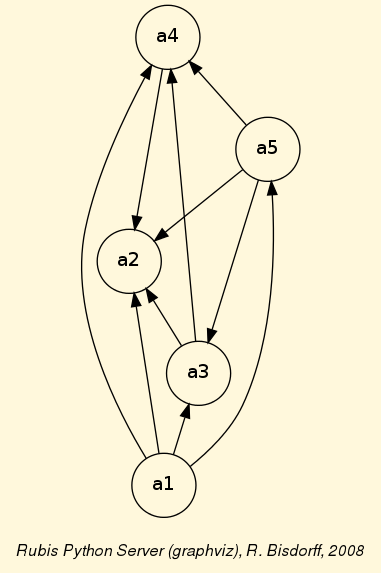
\includegraphics{rel_randLinearProfile.png}
\index{computeArrowRaynaudRanking() (votingDigraphs.CondorcetDigraph method)}

\begin{fulllineitems}
\phantomsection\label{techDoc:votingDigraphs.CondorcetDigraph.computeArrowRaynaudRanking}\pysiglinewithargsret{\bfcode{computeArrowRaynaudRanking}}{\emph{linearOrdered=True}, \emph{Debug=False}}{}
Renders a ranking of the actions following Arrow\&Raynaud's rule.

\end{fulllineitems}

\index{computeCondorcetWinner() (votingDigraphs.CondorcetDigraph method)}

\begin{fulllineitems}
\phantomsection\label{techDoc:votingDigraphs.CondorcetDigraph.computeCondorcetWinner}\pysiglinewithargsret{\bfcode{computeCondorcetWinner}}{}{}
compute the Condorcet winner(s)
renders always a, potentially empty, list

\end{fulllineitems}

\index{computeKohlerRanking() (votingDigraphs.CondorcetDigraph method)}

\begin{fulllineitems}
\phantomsection\label{techDoc:votingDigraphs.CondorcetDigraph.computeKohlerRanking}\pysiglinewithargsret{\bfcode{computeKohlerRanking}}{\emph{linearOrdered=True}, \emph{Debug=False}}{}
Renders a ranking of the actions following Kohler's rule.

\end{fulllineitems}

\index{constructApprovalBallotRelation() (votingDigraphs.CondorcetDigraph method)}

\begin{fulllineitems}
\phantomsection\label{techDoc:votingDigraphs.CondorcetDigraph.constructApprovalBallotRelation}\pysiglinewithargsret{\bfcode{constructApprovalBallotRelation}}{\emph{hasIntegerValuation=False}}{}
Renders the votes differences between candidates
on the basis of an approval ballot.

\end{fulllineitems}

\index{constructBallotRelation() (votingDigraphs.CondorcetDigraph method)}

\begin{fulllineitems}
\phantomsection\label{techDoc:votingDigraphs.CondorcetDigraph.constructBallotRelation}\pysiglinewithargsret{\bfcode{constructBallotRelation}}{\emph{hasIntegerValuation}}{}
Renders the marginal majority between candidates
on the basis of a complete ballot.

\end{fulllineitems}

\index{constructMajorityMarginsRelation() (votingDigraphs.CondorcetDigraph method)}

\begin{fulllineitems}
\phantomsection\label{techDoc:votingDigraphs.CondorcetDigraph.constructMajorityMarginsRelation}\pysiglinewithargsret{\bfcode{constructMajorityMarginsRelation}}{\emph{hasIntegerValuation=True}}{}
Renders the marginal majority between candidates
on the basis of an approval ballot.

\end{fulllineitems}


\end{fulllineitems}

\index{LinearVotingProfile (class in votingDigraphs)}

\begin{fulllineitems}
\phantomsection\label{techDoc:votingDigraphs.LinearVotingProfile}\pysiglinewithargsret{\strong{class }\code{votingDigraphs.}\bfcode{LinearVotingProfile}}{\emph{fileVotingProfile=None}, \emph{numberOfCandidates=5}, \emph{numberOfVoters=9}}{}
Bases: {\hyperref[techDoc:votingDigraphs.VotingProfile]{\code{votingDigraphs.VotingProfile}}}

A specialised class for linear voting profiles

Structure:

\begin{Verbatim}[commandchars=\\\{\}]
candidates = \PYGZob{}\PYGZsq{}a\PYGZsq{}: ,\PYGZsq{}b\PYGZsq{}:  ,\PYGZsq{}c\PYGZsq{}, ..., ...\PYGZcb{}
voters = \PYGZob{}\PYGZsq{}1\PYGZsq{}:\PYGZob{}\PYGZsq{}weight\PYGZsq{}:1.0\PYGZcb{},\PYGZsq{}2\PYGZsq{}:\PYGZob{}\PYGZsq{}weight\PYGZsq{}:1.0\PYGZcb{}, ...\PYGZcb{}
\PYGZsh{}\PYGZsh{} each specifies a a ranked list of candidates
\PYGZsh{}\PYGZsh{} from the best to the worst
linearBallot = \PYGZob{}
    \PYGZsq{}1\PYGZsq{} : [\PYGZsq{}b\PYGZsq{},\PYGZsq{}c\PYGZsq{},\PYGZsq{}a\PYGZsq{}, ...],
    \PYGZsq{}2\PYGZsq{} : [\PYGZsq{}a\PYGZsq{},\PYGZsq{}b\PYGZsq{},\PYGZsq{}c\PYGZsq{}, ...],
    ...
    \PYGZcb{}
\end{Verbatim}

Sample Python3 session

\begin{Verbatim}[commandchars=\\\{\}]
\PYG{g+gp}{\PYGZgt{}\PYGZgt{}\PYGZgt{} }\PYG{k+kn}{from} \PYG{n+nn}{votingDigraphs} \PYG{k+kn}{import} \PYG{o}{*}
\PYG{g+gp}{\PYGZgt{}\PYGZgt{}\PYGZgt{} }\PYG{n}{v} \PYG{o}{=} \PYG{n}{RandomLinearVotingProfile}\PYG{p}{(}\PYG{n}{numberOfVoters}\PYG{o}{=}\PYG{l+m+mi}{5}\PYG{p}{,}\PYG{n}{numberOfCandidates}\PYG{o}{=}\PYG{l+m+mi}{3}\PYG{p}{)}
\PYG{g+gp}{\PYGZgt{}\PYGZgt{}\PYGZgt{} }\PYG{n}{v}\PYG{o}{.}\PYG{n}{showLinearBallots}\PYG{p}{(}\PYG{p}{)}
\PYG{g+go}{voters(weight)       candidates rankings}
\PYG{g+go}{v4(1.0):     [\PYGZsq{}a1\PYGZsq{}, \PYGZsq{}a2\PYGZsq{}, \PYGZsq{}a3\PYGZsq{}]}
\PYG{g+go}{v5(1.0):     [\PYGZsq{}a1\PYGZsq{}, \PYGZsq{}a2\PYGZsq{}, \PYGZsq{}a3\PYGZsq{}]}
\PYG{g+go}{v1(1.0):     [\PYGZsq{}a2\PYGZsq{}, \PYGZsq{}a1\PYGZsq{}, \PYGZsq{}a3\PYGZsq{}]}
\PYG{g+go}{v2(1.0):     [\PYGZsq{}a1\PYGZsq{}, \PYGZsq{}a2\PYGZsq{}, \PYGZsq{}a3\PYGZsq{}]}
\PYG{g+go}{v3(1.0):     [\PYGZsq{}a1\PYGZsq{}, \PYGZsq{}a3\PYGZsq{}, \PYGZsq{}a2\PYGZsq{}]}
\PYG{g+gp}{\PYGZgt{}\PYGZgt{}\PYGZgt{} }\PYG{n}{v}\PYG{o}{.}\PYG{n}{computeRankAnalysis}\PYG{p}{(}\PYG{p}{)}
\PYG{g+go}{\PYGZob{}\PYGZsq{}a1\PYGZsq{}: [4.0, 1.0, 0],}
\PYG{g+go}{ \PYGZsq{}a2\PYGZsq{}: [1.0, 3.0, 1.0],}
\PYG{g+go}{ \PYGZsq{}a3\PYGZsq{}: [0, 1.0, 4.0]]}
\PYG{g+gp}{\PYGZgt{}\PYGZgt{}\PYGZgt{} }\PYG{n}{v}\PYG{o}{.}\PYG{n}{computeUninominalVotes}\PYG{p}{(}\PYG{p}{)}
\PYG{g+go}{\PYGZob{}\PYGZsq{}a1\PYGZsq{}: 4.0, \PYGZsq{}a3\PYGZsq{}: 0, \PYGZsq{}a2\PYGZsq{}: 1.0\PYGZcb{}}
\PYG{g+gp}{\PYGZgt{}\PYGZgt{}\PYGZgt{} }\PYG{n}{v}\PYG{o}{.}\PYG{n}{computeSimpleMajorityWinner}\PYG{p}{(}\PYG{p}{)}
\PYG{g+go}{[\PYGZsq{}a1\PYGZsq{}]}
\PYG{g+gp}{\PYGZgt{}\PYGZgt{}\PYGZgt{} }\PYG{n}{v}\PYG{o}{.}\PYG{n}{computeBordaScores}\PYG{p}{(}\PYG{p}{)}
\PYG{g+go}{\PYGZob{}\PYGZsq{}a1\PYGZsq{}: 6.0, \PYGZsq{}a3\PYGZsq{}: 14.0, \PYGZsq{}a2\PYGZsq{}: 10.0\PYGZcb{}}
\PYG{g+gp}{\PYGZgt{}\PYGZgt{}\PYGZgt{} }\PYG{n}{v}\PYG{o}{.}\PYG{n}{computeBordaWinners}\PYG{p}{(}\PYG{p}{)}
\PYG{g+go}{[\PYGZsq{}a1\PYGZsq{}]}
\PYG{g+gp}{\PYGZgt{}\PYGZgt{}\PYGZgt{} }\PYG{n}{v}\PYG{o}{.}\PYG{n}{computeInstantRunoffWinner}\PYG{p}{(}\PYG{p}{)}
\PYG{g+go}{[\PYGZsq{}a1\PYGZsq{}]}
\end{Verbatim}
\index{computeBallot() (votingDigraphs.LinearVotingProfile method)}

\begin{fulllineitems}
\phantomsection\label{techDoc:votingDigraphs.LinearVotingProfile.computeBallot}\pysiglinewithargsret{\bfcode{computeBallot}}{}{}
Computes a complete ballot from the linear Ballot.

\end{fulllineitems}

\index{computeBordaScores() (votingDigraphs.LinearVotingProfile method)}

\begin{fulllineitems}
\phantomsection\label{techDoc:votingDigraphs.LinearVotingProfile.computeBordaScores}\pysiglinewithargsret{\bfcode{computeBordaScores}}{}{}
compute Borda scores from the rank analysis

\end{fulllineitems}

\index{computeBordaWinners() (votingDigraphs.LinearVotingProfile method)}

\begin{fulllineitems}
\phantomsection\label{techDoc:votingDigraphs.LinearVotingProfile.computeBordaWinners}\pysiglinewithargsret{\bfcode{computeBordaWinners}}{}{}
compute the Borda winner from the Borda scores, ie the list of
candidates with the minimal Borda score.

\end{fulllineitems}

\index{computeInstantRunoffWinner() (votingDigraphs.LinearVotingProfile method)}

\begin{fulllineitems}
\phantomsection\label{techDoc:votingDigraphs.LinearVotingProfile.computeInstantRunoffWinner}\pysiglinewithargsret{\bfcode{computeInstantRunoffWinner}}{\emph{Comments=False}}{}
compute the instant runoff winner from a linear voting ballot

\end{fulllineitems}

\index{computeRankAnalysis() (votingDigraphs.LinearVotingProfile method)}

\begin{fulllineitems}
\phantomsection\label{techDoc:votingDigraphs.LinearVotingProfile.computeRankAnalysis}\pysiglinewithargsret{\bfcode{computeRankAnalysis}}{}{}
compute the number of ranks each candidate obtains

\end{fulllineitems}

\index{computeSimpleMajorityWinner() (votingDigraphs.LinearVotingProfile method)}

\begin{fulllineitems}
\phantomsection\label{techDoc:votingDigraphs.LinearVotingProfile.computeSimpleMajorityWinner}\pysiglinewithargsret{\bfcode{computeSimpleMajorityWinner}}{\emph{Comments=False}}{}
compute the winner in a uninominal Election from a linear ballot

\end{fulllineitems}

\index{computeUninominalVotes() (votingDigraphs.LinearVotingProfile method)}

\begin{fulllineitems}
\phantomsection\label{techDoc:votingDigraphs.LinearVotingProfile.computeUninominalVotes}\pysiglinewithargsret{\bfcode{computeUninominalVotes}}{\emph{candidates=None}, \emph{linearBallot=None}}{}
compute uninominal votes for each candidate in candidates sublist
and restricted linear ballots

\end{fulllineitems}

\index{save() (votingDigraphs.LinearVotingProfile method)}

\begin{fulllineitems}
\phantomsection\label{techDoc:votingDigraphs.LinearVotingProfile.save}\pysiglinewithargsret{\bfcode{save}}{\emph{name='templinearprofile'}}{}
Persistant storage of a linear voting profile.
\begin{description}
\item[{Parameter:}] \leavevmode
name of file (without \textless{}.py\textgreater{} extension!).

\end{description}

\end{fulllineitems}

\index{showLinearBallots() (votingDigraphs.LinearVotingProfile method)}

\begin{fulllineitems}
\phantomsection\label{techDoc:votingDigraphs.LinearVotingProfile.showLinearBallots}\pysiglinewithargsret{\bfcode{showLinearBallots}}{}{}
show the linear ballots

\end{fulllineitems}


\end{fulllineitems}

\index{RandomApprovalVotingProfile (class in votingDigraphs)}

\begin{fulllineitems}
\phantomsection\label{techDoc:votingDigraphs.RandomApprovalVotingProfile}\pysiglinewithargsret{\strong{class }\code{votingDigraphs.}\bfcode{RandomApprovalVotingProfile}}{\emph{numberOfVoters=9}, \emph{numberOfCandidates=5}, \emph{minSizeOfBallot=1}, \emph{maxSizeOfBallot=2}}{}
Bases: {\hyperref[techDoc:votingDigraphs.ApprovalVotingProfile]{\code{votingDigraphs.ApprovalVotingProfile}}}

A specialized class for approval voting profiles.
\index{generateRandomApprovalBallot() (votingDigraphs.RandomApprovalVotingProfile method)}

\begin{fulllineitems}
\phantomsection\label{techDoc:votingDigraphs.RandomApprovalVotingProfile.generateRandomApprovalBallot}\pysiglinewithargsret{\bfcode{generateRandomApprovalBallot}}{\emph{minSizeOfBallot}, \emph{maxSizeOfBallot}}{}
Renders a randomly generated approval ballot.

\end{fulllineitems}


\end{fulllineitems}

\index{RandomLinearVotingProfile (class in votingDigraphs)}

\begin{fulllineitems}
\phantomsection\label{techDoc:votingDigraphs.RandomLinearVotingProfile}\pysiglinewithargsret{\strong{class }\code{votingDigraphs.}\bfcode{RandomLinearVotingProfile}}{\emph{seed=None}, \emph{numberOfVoters=9}, \emph{numberOfCandidates=5}}{}
Bases: {\hyperref[techDoc:votingDigraphs.LinearVotingProfile]{\code{votingDigraphs.LinearVotingProfile}}}

A specialized class for random linwear voting profiles.
\index{generateRandomLinearBallot() (votingDigraphs.RandomLinearVotingProfile method)}

\begin{fulllineitems}
\phantomsection\label{techDoc:votingDigraphs.RandomLinearVotingProfile.generateRandomLinearBallot}\pysiglinewithargsret{\bfcode{generateRandomLinearBallot}}{\emph{seed}}{}
Renders a randomly generated linear ballot.

\end{fulllineitems}


\end{fulllineitems}

\index{RandomVotingProfile (class in votingDigraphs)}

\begin{fulllineitems}
\phantomsection\label{techDoc:votingDigraphs.RandomVotingProfile}\pysiglinewithargsret{\strong{class }\code{votingDigraphs.}\bfcode{RandomVotingProfile}}{\emph{numberOfVoters=9}, \emph{numberOfCandidates=5}, \emph{hasRandomWeights=False}, \emph{maxWeight=10}, \emph{seed=None}, \emph{Debug=False}}{}
Bases: {\hyperref[techDoc:votingDigraphs.VotingProfile]{\code{votingDigraphs.VotingProfile}}}

A subclass for generating random voting profiles.
\index{generateRandomBallot() (votingDigraphs.RandomVotingProfile method)}

\begin{fulllineitems}
\phantomsection\label{techDoc:votingDigraphs.RandomVotingProfile.generateRandomBallot}\pysiglinewithargsret{\bfcode{generateRandomBallot}}{\emph{seed}, \emph{Debug=False}}{}
Renders a randomly generated approval ballot
from a shuffled list of candidates for each voter.

\end{fulllineitems}


\end{fulllineitems}

\index{VotingProfile (class in votingDigraphs)}

\begin{fulllineitems}
\phantomsection\label{techDoc:votingDigraphs.VotingProfile}\pysiglinewithargsret{\strong{class }\code{votingDigraphs.}\bfcode{VotingProfile}}{\emph{fileVotingProfile=None}}{}
Bases: \code{builtins.object}

A general class for storing voting profiles.

General structure:

\begin{Verbatim}[commandchars=\\\{\}]
candidates = \PYGZob{}\PYGZsq{}a\PYGZsq{}: ...,\PYGZsq{}b\PYGZsq{}: ...,\PYGZsq{}c\PYGZsq{}: ...,  ... \PYGZcb{}
voters = \PYGZob{}
\PYGZsq{}1\PYGZsq{}:\PYGZob{}\PYGZsq{}weight\PYGZsq{}:1.0\PYGZcb{},
\PYGZsq{}2\PYGZsq{}:\PYGZob{}\PYGZsq{}weight\PYGZsq{}:1.0\PYGZcb{},
...,
\PYGZcb{}
ballot = \PYGZob{}     \PYGZsh{} voters x candidates x candidates
    \PYGZsq{}1\PYGZsq{}: \PYGZob{}     \PYGZsh{} bipolar characteristic \PYGZob{}\PYGZhy{}1,0,1\PYGZcb{} of each voter\PYGZsq{}s
          \PYGZsq{}a\PYGZsq{}: \PYGZob{} \PYGZsq{}a\PYGZsq{}:0,\PYGZsq{}b\PYGZsq{}:\PYGZhy{}1,\PYGZsq{}c\PYGZsq{}:0, ...\PYGZcb{},   \PYGZsh{} pairwise preferences
          \PYGZsq{}b\PYGZsq{}: \PYGZob{} \PYGZsq{}a\PYGZsq{}:1,\PYGZsq{}b\PYGZsq{}:0, \PYGZsq{}c\PYGZsq{}:1, ...\PYGZcb{},
          \PYGZsq{}c\PYGZsq{}: \PYGZob{} \PYGZsq{}a\PYGZsq{}:0,\PYGZsq{}b\PYGZsq{}:\PYGZhy{}1,\PYGZsq{}c\PYGZsq{}:0, ...\PYGZcb{},
          ...,
    \PYGZcb{},
    \PYGZsq{}2\PYGZsq{}: \PYGZob{} \PYGZsq{}a\PYGZsq{}: \PYGZob{} \PYGZsq{}a\PYGZsq{}:0, \PYGZsq{}b\PYGZsq{}:0, \PYGZsq{}c\PYGZsq{}:1, ...\PYGZcb{},
           \PYGZsq{}b\PYGZsq{}: \PYGZob{} \PYGZsq{}a\PYGZsq{}:0, \PYGZsq{}b\PYGZsq{}:0, \PYGZsq{}c\PYGZsq{}:1, ...\PYGZcb{},
           \PYGZsq{}c\PYGZsq{}: \PYGZob{} \PYGZsq{}a\PYGZsq{}:\PYGZhy{}1,\PYGZsq{}b\PYGZsq{}:\PYGZhy{}1,\PYGZsq{}c\PYGZsq{}:0, ...\PYGZcb{},
           ...,
    \PYGZcb{},
    ...,
\PYGZcb{}
\end{Verbatim}
\index{save() (votingDigraphs.VotingProfile method)}

\begin{fulllineitems}
\phantomsection\label{techDoc:votingDigraphs.VotingProfile.save}\pysiglinewithargsret{\bfcode{save}}{\emph{name='tempVprofile'}}{}
Persistant storage of an approval voting profile.

\end{fulllineitems}

\index{showAll() (votingDigraphs.VotingProfile method)}

\begin{fulllineitems}
\phantomsection\label{techDoc:votingDigraphs.VotingProfile.showAll}\pysiglinewithargsret{\bfcode{showAll}}{\emph{WithBallots=True}}{}
Show method for \textless{}VotingProfile\textgreater{} instances.

\end{fulllineitems}

\index{showVoterBallot() (votingDigraphs.VotingProfile method)}

\begin{fulllineitems}
\phantomsection\label{techDoc:votingDigraphs.VotingProfile.showVoterBallot}\pysiglinewithargsret{\bfcode{showVoterBallot}}{\emph{voter}, \emph{hasIntegerValuation=False}}{}
Show the actual voting of a voter.

\end{fulllineitems}


\end{fulllineitems}


Back to the {\hyperref[techDoc:introduction-label]{\emph{Introduction}}}


\subsection{sortingDigraphs module}
\label{techDoc:sortingdigraphs-label}\label{techDoc:module-sortingDigraphs}\label{techDoc:sortingdigraphs-module}\index{sortingDigraphs (module)}\index{OptimalQuantilesSortingDigraph (class in sortingDigraphs)}

\begin{fulllineitems}
\phantomsection\label{techDoc:sortingDigraphs.OptimalQuantilesSortingDigraph}\pysiglinewithargsret{\strong{class }\code{sortingDigraphs.}\bfcode{OptimalQuantilesSortingDigraph}}{\emph{argPerfTab=None}, \emph{minQuantiles=4}, \emph{maxQuantiles=50}, \emph{LowerClosed=True}, \emph{PrefThresholds=True}, \emph{hasNoVeto=False}, \emph{minValuation=-100.0}, \emph{maxValuation=100.0}, \emph{outrankingType='bipolar'}, \emph{Prudent=False}, \emph{Threading=False}, \emph{Debug=False}}{}
Bases: {\hyperref[techDoc:sortingDigraphs.QuantilesSortingDigraph]{\code{sortingDigraphs.QuantilesSortingDigraph}}}

Specialisation of the QuantilesSortingDigraph Class
for optimal sorting of alternatives into
quantiles delimited ordered classes.

\end{fulllineitems}

\index{QuantilesSortingDigraph (class in sortingDigraphs)}

\begin{fulllineitems}
\phantomsection\label{techDoc:sortingDigraphs.QuantilesSortingDigraph}\pysiglinewithargsret{\strong{class }\code{sortingDigraphs.}\bfcode{QuantilesSortingDigraph}}{\emph{argPerfTab=None}, \emph{limitingQuantiles=None}, \emph{LowerClosed=True}, \emph{PrefThresholds=True}, \emph{hasNoVeto=False}, \emph{minValuation=-1.0}, \emph{maxValuation=1.0}, \emph{outrankingType='bipolar'}, \emph{CompleteOutranking=True}, \emph{Threading=False}, \emph{Debug=False}}{}
Bases: {\hyperref[techDoc:sortingDigraphs.SortingDigraph]{\code{sortingDigraphs.SortingDigraph}}}, {\hyperref[techDoc:weakOrders.WeakOrder]{\code{weakOrders.WeakOrder}}}

Specialisation of the sortingDigraph Class
for sorting of alternatives into quantiles delimited ordered classes.

\begin{notice}{note}{Note:}
We generally require an PerformanceTableau instance or a valid filename.
If none is given, then a default profile with the limiting quartiles Q0,Q1,Q2, Q3 and Q4 is used on each criteria.
By default lower closed limits of categories are supposed to be used in the sorting.
\end{notice}

Example Python3 session:

\begin{Verbatim}[commandchars=\\\{\}]
\PYG{g+gp}{\PYGZgt{}\PYGZgt{}\PYGZgt{} }\PYG{k+kn}{from} \PYG{n+nn}{sortingDigraphs} \PYG{k+kn}{import} \PYG{o}{*}
\PYG{g+gp}{\PYGZgt{}\PYGZgt{}\PYGZgt{} }\PYG{n}{t} \PYG{o}{=} \PYG{n}{RandomCBPerformanceTableau}\PYG{p}{(}\PYG{n}{numberOfActions}\PYG{o}{=}\PYG{l+m+mi}{7}\PYG{p}{,}\PYG{n}{numberOfCriteria}\PYG{o}{=}\PYG{l+m+mi}{5}\PYG{p}{,}
\PYG{g+gp}{... }                               \PYG{n}{weightDistribution}\PYG{o}{=}\PYG{l+s}{\PYGZsq{}}\PYG{l+s}{equiobjectives}\PYG{l+s}{\PYGZsq{}}\PYG{p}{)}
\PYG{g+gp}{\PYGZgt{}\PYGZgt{}\PYGZgt{} }\PYG{n}{qs} \PYG{o}{=} \PYG{n}{QuantilesSortingDigraph}\PYG{p}{(}\PYG{n}{t}\PYG{p}{,}\PYG{n}{limitingQuantiles}\PYG{o}{=}\PYG{l+m+mi}{10}\PYG{p}{)}
\PYG{g+gp}{\PYGZgt{}\PYGZgt{}\PYGZgt{} }\PYG{n}{qs}\PYG{o}{.}\PYG{n}{showSorting}\PYG{p}{(}\PYG{p}{)}
\PYG{g+go}{*\PYGZhy{}\PYGZhy{}\PYGZhy{} Sorting results in descending order \PYGZhy{}\PYGZhy{}\PYGZhy{}*}
\PYG{g+go}{[0.90 \PYGZhy{} \PYGZlt{}[:          []}
\PYG{g+go}{[0.80 \PYGZhy{} 0.90[:       []}
\PYG{g+go}{[0.70 \PYGZhy{} 0.80[:       []}
\PYG{g+go}{[0.60 \PYGZhy{} 0.70[:       [\PYGZsq{}a02\PYGZsq{}, \PYGZsq{}a07\PYGZsq{}]}
\PYG{g+go}{[0.50 \PYGZhy{} 0.60[:       [\PYGZsq{}a02\PYGZsq{}, \PYGZsq{}a04\PYGZsq{}, \PYGZsq{}a05\PYGZsq{}, \PYGZsq{}a06\PYGZsq{}]}
\PYG{g+go}{[0.40 \PYGZhy{} 0.50[:       []}
\PYG{g+go}{[0.30 \PYGZhy{} 0.40[:       []}
\PYG{g+go}{[0.20 \PYGZhy{} 0.30[:       [\PYGZsq{}a03\PYGZsq{}]}
\PYG{g+go}{[0.10 \PYGZhy{} 0.20[:       [\PYGZsq{}a01\PYGZsq{}]}
\PYG{g+go}{[0.00 \PYGZhy{} 0.10[:       []}
\PYG{g+gp}{\PYGZgt{}\PYGZgt{}\PYGZgt{} }\PYG{n}{qs}\PYG{o}{.}\PYG{n}{exportGraphViz}\PYG{p}{(}\PYG{l+s}{\PYGZsq{}}\PYG{l+s}{quantilesSorting}\PYG{l+s}{\PYGZsq{}}\PYG{p}{)}
\end{Verbatim}

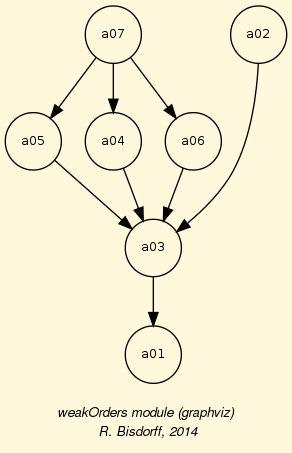
\includegraphics{quantilesSorting.png}
\index{computeSortingRelation() (sortingDigraphs.QuantilesSortingDigraph method)}

\begin{fulllineitems}
\phantomsection\label{techDoc:sortingDigraphs.QuantilesSortingDigraph.computeSortingRelation}\pysiglinewithargsret{\bfcode{computeSortingRelation}}{\emph{categoryContents=None}, \emph{Debug=False}}{}
constructs a bipolar sorting relation using the category contents.

\end{fulllineitems}

\index{showActionCategories() (sortingDigraphs.QuantilesSortingDigraph method)}

\begin{fulllineitems}
\phantomsection\label{techDoc:sortingDigraphs.QuantilesSortingDigraph.showActionCategories}\pysiglinewithargsret{\bfcode{showActionCategories}}{\emph{action}, \emph{Debug=False}, \emph{Comments=True}}{}
Renders the union of categories in which the given action is sorted positively or null into.
Returns a tuple : action, lowest category key, highest category key, membership credibility !

\end{fulllineitems}

\index{showActionsSortingResult() (sortingDigraphs.QuantilesSortingDigraph method)}

\begin{fulllineitems}
\phantomsection\label{techDoc:sortingDigraphs.QuantilesSortingDigraph.showActionsSortingResult}\pysiglinewithargsret{\bfcode{showActionsSortingResult}}{\emph{actionSubset=None}}{}
shows the quantiles sorting result all (default) of a subset of the decision actions.

\end{fulllineitems}

\index{showSorting() (sortingDigraphs.QuantilesSortingDigraph method)}

\begin{fulllineitems}
\phantomsection\label{techDoc:sortingDigraphs.QuantilesSortingDigraph.showSorting}\pysiglinewithargsret{\bfcode{showSorting}}{\emph{Reverse=True}, \emph{isReturningHTML=False}, \emph{Debug=False}}{}
Shows sorting results in decreasing or increasing (Reverse=False)
order of the categories. If isReturningHTML is True (default = False)
the method returns a htlm table with the sorting result.

\end{fulllineitems}

\index{showWeakOrder() (sortingDigraphs.QuantilesSortingDigraph method)}

\begin{fulllineitems}
\phantomsection\label{techDoc:sortingDigraphs.QuantilesSortingDigraph.showWeakOrder}\pysiglinewithargsret{\bfcode{showWeakOrder}}{\emph{Descending=True}}{}
Specialisation for QauntilesSortingDigraphs.

\end{fulllineitems}


\end{fulllineitems}

\index{SortingDigraph (class in sortingDigraphs)}

\begin{fulllineitems}
\phantomsection\label{techDoc:sortingDigraphs.SortingDigraph}\pysiglinewithargsret{\strong{class }\code{sortingDigraphs.}\bfcode{SortingDigraph}}{\emph{argPerfTab=None}, \emph{argProfile=None}, \emph{scaleSteps=5}, \emph{minValuation=-100.0}, \emph{maxValuation=100.0}, \emph{isRobust=False}, \emph{hasNoVeto=False}, \emph{lowerClosed=True}, \emph{Threading=False}, \emph{Debug=False}}{}
Bases: {\hyperref[techDoc:outrankingDigraphs.BipolarOutrankingDigraph]{\code{outrankingDigraphs.BipolarOutrankingDigraph}}}, {\hyperref[techDoc:perfTabs.PerformanceTableau]{\code{perfTabs.PerformanceTableau}}}

Specialisation of the digraphs.BipolarOutrankingDigraph Class
for Condorcet based multicriteria sorting of alternatives.

Besides a valid PerformanceTableau instance we require a sorting profile,
i.e.:
\begin{itemize}
\item {} 
a dictionary \textless{}categories\textgreater{} of categories with `name', `order' and `comment'

\item {} 
a dictionary \textless{}criteriaCategoryLimits\textgreater{} with double entry:
\begin{quote}

{[}criteriakey{]}{[}categoryKey{]} containing a {[}'minimum'{]} and
a  {[}'maximum'{]} value in the scale of the criterion
respecting the order of the categories.
\end{quote}

\end{itemize}

Template of required data:

\begin{Verbatim}[commandchars=\\\{\}]
\PYG{n+nb+bp}{self}\PYG{o}{.}\PYG{n}{categories} \PYG{o}{=} \PYG{p}{\PYGZob{}}\PYG{l+s}{\PYGZsq{}}\PYG{l+s}{c01}\PYG{l+s}{\PYGZsq{}}\PYG{p}{:} \PYG{p}{\PYGZob{}} \PYG{l+s}{\PYGZsq{}}\PYG{l+s}{name}\PYG{l+s}{\PYGZsq{}}\PYG{p}{:} \PYG{l+s}{\PYGZsq{}}\PYG{l+s}{week}\PYG{l+s}{\PYGZsq{}}\PYG{p}{,}\PYG{l+s}{\PYGZsq{}}\PYG{l+s}{order}\PYG{l+s}{\PYGZsq{}}\PYG{p}{:} \PYG{l+m+mi}{0}\PYG{p}{,}
                            \PYG{l+s}{\PYGZsq{}}\PYG{l+s}{comment}\PYG{l+s}{\PYGZsq{}}\PYG{p}{:} \PYG{l+s}{\PYGZsq{}}\PYG{l+s}{lowest category}\PYG{l+s}{\PYGZsq{}}\PYG{p}{,}\PYG{p}{\PYGZcb{}}\PYG{p}{,}
                   \PYG{l+s}{\PYGZsq{}}\PYG{l+s}{c02}\PYG{l+s}{\PYGZsq{}}\PYG{p}{:} \PYG{p}{\PYGZob{}} \PYG{l+s}{\PYGZsq{}}\PYG{l+s}{name}\PYG{l+s}{\PYGZsq{}}\PYG{p}{:} \PYG{l+s}{\PYGZsq{}}\PYG{l+s}{ok}\PYG{l+s}{\PYGZsq{}}\PYG{p}{,}\PYG{l+s}{\PYGZsq{}}\PYG{l+s}{order}\PYG{l+s}{\PYGZsq{}}\PYG{p}{:} \PYG{l+m+mi}{1}\PYG{p}{,}
                            \PYG{l+s}{\PYGZsq{}}\PYG{l+s}{comment}\PYG{l+s}{\PYGZsq{}}\PYG{p}{:} \PYG{l+s}{\PYGZsq{}}\PYG{l+s}{medium category}\PYG{l+s}{\PYGZsq{}}\PYG{p}{,}\PYG{p}{\PYGZcb{}}\PYG{p}{,}
                   \PYG{l+s}{\PYGZsq{}}\PYG{l+s}{c03}\PYG{l+s}{\PYGZsq{}}\PYG{p}{:} \PYG{p}{\PYGZob{}} \PYG{l+s}{\PYGZsq{}}\PYG{l+s}{name}\PYG{l+s}{\PYGZsq{}}\PYG{p}{:} \PYG{l+s}{\PYGZsq{}}\PYG{l+s}{good}\PYG{l+s}{\PYGZsq{}}\PYG{p}{,}\PYG{l+s}{\PYGZsq{}}\PYG{l+s}{order}\PYG{l+s}{\PYGZsq{}}\PYG{p}{:} \PYG{l+m+mi}{2}\PYG{p}{,}
                            \PYG{l+s}{\PYGZsq{}}\PYG{l+s}{comment}\PYG{l+s}{\PYGZsq{}}\PYG{p}{:} \PYG{l+s}{\PYGZsq{}}\PYG{l+s}{highest category}\PYG{l+s}{\PYGZsq{}}\PYG{p}{,}\PYG{p}{\PYGZcb{}}\PYG{p}{,}
                   \PYG{l+s}{\PYGZsq{}}\PYG{l+s}{c04}\PYG{l+s}{\PYGZsq{}}\PYG{p}{:} \PYG{p}{\PYGZob{}} \PYG{l+s}{\PYGZsq{}}\PYG{l+s}{name}\PYG{l+s}{\PYGZsq{}}\PYG{p}{:} \PYG{l+s}{\PYGZsq{}}\PYG{l+s}{excellent}\PYG{l+s}{\PYGZsq{}}\PYG{p}{,}\PYG{l+s}{\PYGZsq{}}\PYG{l+s}{order}\PYG{l+s}{\PYGZsq{}}\PYG{p}{:} \PYG{l+m+mi}{3}\PYG{p}{,}
                            \PYG{l+s}{\PYGZsq{}}\PYG{l+s}{comment}\PYG{l+s}{\PYGZsq{}}\PYG{p}{:} \PYG{l+s}{\PYGZsq{}}\PYG{l+s}{highest category}\PYG{l+s}{\PYGZsq{}}\PYG{p}{,}\PYG{p}{\PYGZcb{}}\PYG{p}{,}
\PYG{p}{\PYGZcb{}}
\PYG{n+nb+bp}{self}\PYG{o}{.}\PYG{n}{criteriaCategoryLimits}\PYG{p}{[}\PYG{l+s}{\PYGZsq{}}\PYG{l+s}{lowerClosed}\PYG{l+s}{\PYGZsq{}}\PYG{p}{]} \PYG{o}{=} \PYG{n+nb+bp}{True} \PYG{c}{\PYGZsh{} default}
\PYG{n+nb+bp}{self}\PYG{o}{.}\PYG{n}{criteriaCategoryLimits}\PYG{p}{[}\PYG{n}{g}\PYG{p}{]} \PYG{o}{=} \PYG{p}{\PYGZob{}}
        \PYG{l+s}{\PYGZsq{}}\PYG{l+s}{c01}\PYG{l+s}{\PYGZsq{}}\PYG{p}{:} \PYG{p}{\PYGZob{}}\PYG{l+s}{\PYGZsq{}}\PYG{l+s}{minimum}\PYG{l+s}{\PYGZsq{}}\PYG{p}{:}\PYG{l+m+mi}{0}\PYG{p}{,} \PYG{l+s}{\PYGZsq{}}\PYG{l+s}{maximum}\PYG{l+s}{\PYGZsq{}}\PYG{p}{:}\PYG{l+m+mi}{25}\PYG{p}{\PYGZcb{}}\PYG{p}{,}
        \PYG{l+s}{\PYGZsq{}}\PYG{l+s}{c02}\PYG{l+s}{\PYGZsq{}}\PYG{p}{:} \PYG{p}{\PYGZob{}}\PYG{l+s}{\PYGZsq{}}\PYG{l+s}{minimum}\PYG{l+s}{\PYGZsq{}}\PYG{p}{:}\PYG{l+m+mi}{25}\PYG{p}{,} \PYG{l+s}{\PYGZsq{}}\PYG{l+s}{maximum}\PYG{l+s}{\PYGZsq{}}\PYG{p}{:}\PYG{l+m+mi}{50}\PYG{p}{\PYGZcb{}}\PYG{p}{,}
        \PYG{l+s}{\PYGZsq{}}\PYG{l+s}{c03}\PYG{l+s}{\PYGZsq{}}\PYG{p}{:} \PYG{p}{\PYGZob{}}\PYG{l+s}{\PYGZsq{}}\PYG{l+s}{minimum}\PYG{l+s}{\PYGZsq{}}\PYG{p}{:}\PYG{l+m+mi}{50}\PYG{p}{,} \PYG{l+s}{\PYGZsq{}}\PYG{l+s}{maximum}\PYG{l+s}{\PYGZsq{}}\PYG{p}{:}\PYG{l+m+mi}{75}\PYG{p}{\PYGZcb{}}\PYG{p}{,}
        \PYG{l+s}{\PYGZsq{}}\PYG{l+s}{c04}\PYG{l+s}{\PYGZsq{}}\PYG{p}{:} \PYG{p}{\PYGZob{}}\PYG{l+s}{\PYGZsq{}}\PYG{l+s}{minimum}\PYG{l+s}{\PYGZsq{}}\PYG{p}{:}\PYG{l+m+mi}{75}\PYG{p}{,} \PYG{l+s}{\PYGZsq{}}\PYG{l+s}{maximum}\PYG{l+s}{\PYGZsq{}}\PYG{p}{:}\PYG{l+m+mi}{120}\PYG{p}{\PYGZcb{}}\PYG{p}{,}
 \PYG{p}{\PYGZcb{}}
\end{Verbatim}

A template named tempProfile.py is providied in the digraphs module distribution.

\begin{notice}{note}{Note:}
We generally require a performanceTableau instance and a filename
where categories and a profile my be read from. If no such filename is given,
then a default profile with five, equally spaced, categories is used
on each criteria. By default lower-closed limts of categories are
supposed to be used in the sorting.If no performance tableau instance is given,
a standard random instance with 10 actions and 13 criteria is generated by default.
\end{notice}

Example Python3 session

\begin{Verbatim}[commandchars=\\\{\}]
\PYG{g+gp}{\PYGZgt{}\PYGZgt{}\PYGZgt{} }\PYG{k+kn}{from} \PYG{n+nn}{sortingDigraphs} \PYG{k+kn}{import} \PYG{n}{SortingDigraph}
\PYG{g+gp}{\PYGZgt{}\PYGZgt{}\PYGZgt{} }\PYG{n}{s} \PYG{o}{=} \PYG{n}{SortingDigraph}\PYG{p}{(}\PYG{p}{)} \PYG{o}{\PYGZpc{}}\PYG{o}{\PYGZpc{}} \PYG{n}{Based} \PYG{n}{on} \PYG{n}{a} \PYG{n}{random} \PYG{n}{performance} \PYG{n}{tableau} 
\PYG{g+gp}{\PYGZgt{}\PYGZgt{}\PYGZgt{} }\PYG{p}{[}\PYG{n}{x} \PYG{k}{for} \PYG{n}{x} \PYG{o+ow}{in} \PYG{n}{s}\PYG{o}{.}\PYG{n}{actions}\PYG{p}{]}
\PYG{g+go}{[\PYGZsq{}a07\PYGZsq{}, \PYGZsq{}a06\PYGZsq{}, \PYGZsq{}a05\PYGZsq{}, \PYGZsq{}a04\PYGZsq{}, \PYGZsq{}a03\PYGZsq{}, \PYGZsq{}a02\PYGZsq{}, \PYGZsq{}a01\PYGZsq{}, \PYGZsq{}a10\PYGZsq{}, \PYGZsq{}a09\PYGZsq{}, \PYGZsq{}a08\PYGZsq{}]}
\PYG{g+gp}{\PYGZgt{}\PYGZgt{}\PYGZgt{} }\PYG{n}{s}\PYG{o}{.}\PYG{n}{showSorting}\PYG{p}{(}\PYG{p}{)}
\PYG{g+go}{*\PYGZhy{}\PYGZhy{}\PYGZhy{} Sorting results in descending order \PYGZhy{}\PYGZhy{}\PYGZhy{}*}
\PYG{g+go}{]\PYGZgt{} \PYGZhy{} 100]:   []}
\PYG{g+go}{]100 \PYGZhy{} 80]:  [\PYGZsq{}a03\PYGZsq{}, \PYGZsq{}a09\PYGZsq{}]}
\PYG{g+go}{]80 \PYGZhy{} 60]:   [\PYGZsq{}a02\PYGZsq{}, \PYGZsq{}a04\PYGZsq{}, \PYGZsq{}a05\PYGZsq{}, \PYGZsq{}a06\PYGZsq{}, \PYGZsq{}a07\PYGZsq{}, \PYGZsq{}a08\PYGZsq{}]}
\PYG{g+go}{]60 \PYGZhy{} 40]:   [\PYGZsq{}a01\PYGZsq{}, \PYGZsq{}a10\PYGZsq{}]}
\PYG{g+go}{]40 \PYGZhy{} 20]:   []}
\PYG{g+go}{]20 \PYGZhy{} 0]:    []}
\PYG{g+gp}{\PYGZgt{}\PYGZgt{}\PYGZgt{} }\PYG{n}{s}\PYG{o}{.}\PYG{n}{showSortingCharacteristics}\PYG{p}{(}\PYG{l+s}{\PYGZsq{}}\PYG{l+s}{a10}\PYG{l+s}{\PYGZsq{}}\PYG{p}{)}
\PYG{g+go}{x  in  K\PYGZus{}k    r(x \PYGZgt{}= m\PYGZus{}k)   r(x \PYGZlt{} M\PYGZus{}k)  r(x in K\PYGZus{}k)}
\PYG{g+go}{a10 in [0\PYGZhy{}20[    100.00      \PYGZhy{}85.98       \PYGZhy{}85.98}
\PYG{g+go}{a10 in [20\PYGZhy{}40[    85.98      \PYGZhy{}49.53       \PYGZhy{}49.53}
\PYG{g+go}{a10 in [40\PYGZhy{}60[    49.53       20.56        20.56}
\PYG{g+go}{a10 in [60\PYGZhy{}80[   \PYGZhy{}20.56       34.58       \PYGZhy{}20.56}
\PYG{g+go}{a10 in [80\PYGZhy{}100[  \PYGZhy{}34.58      100.00       \PYGZhy{}34.58}
\PYG{g+go}{a10 in [100\PYGZhy{}\PYGZlt{}[  \PYGZhy{}100.00      100.00      \PYGZhy{}100.00}
\PYG{g+gp}{\PYGZgt{}\PYGZgt{}\PYGZgt{} }\PYG{k+kn}{from} \PYG{n+nn}{outrankingDigraphs} \PYG{k+kn}{import} \PYG{n}{BipolarOutrankingDigraph}
\PYG{g+gp}{\PYGZgt{}\PYGZgt{}\PYGZgt{} }\PYG{n}{g} \PYG{o}{=} \PYG{n}{BipolarOutrankingDigraph}\PYG{p}{(}\PYG{n}{s}\PYG{p}{)}
\PYG{g+gp}{\PYGZgt{}\PYGZgt{}\PYGZgt{} }\PYG{n}{g}\PYG{o}{.}\PYG{n}{computeOrdinalCorrelation}\PYG{p}{(}\PYG{n}{s}\PYG{p}{)}
\PYG{g+go}{\PYGZob{}\PYGZsq{}determination\PYGZsq{}: Decimal(\PYGZsq{}0.2438213914849428868120456904\PYGZsq{}),}
\PYG{g+go}{\PYGZsq{}MedianCut\PYGZsq{}: False,}
\PYG{g+go}{\PYGZsq{}correlation\PYGZsq{}: Decimal(\PYGZsq{}0.6482112436115843270868824533\PYGZsq{})\PYGZcb{}}
\PYG{g+gp}{\PYGZgt{}\PYGZgt{}\PYGZgt{} }
\end{Verbatim}
\index{computeCategoryContents() (sortingDigraphs.SortingDigraph method)}

\begin{fulllineitems}
\phantomsection\label{techDoc:sortingDigraphs.SortingDigraph.computeCategoryContents}\pysiglinewithargsret{\bfcode{computeCategoryContents}}{\emph{Reverse=False}, \emph{Comments=False}}{}
Computes the sorting results per category.

\end{fulllineitems}

\index{computeSortingCharacteristics() (sortingDigraphs.SortingDigraph method)}

\begin{fulllineitems}
\phantomsection\label{techDoc:sortingDigraphs.SortingDigraph.computeSortingCharacteristics}\pysiglinewithargsret{\bfcode{computeSortingCharacteristics}}{\emph{action=None}, \emph{Comments=False}}{}
Renders a bipolar-valued bi-dictionary relation
representing the degree of credibility of the
assertion that ``action x in A belongs to category c in C'',
ie x outranks low category limit and does not outrank
the high category limit.

\end{fulllineitems}

\index{computeSortingRelation() (sortingDigraphs.SortingDigraph method)}

\begin{fulllineitems}
\phantomsection\label{techDoc:sortingDigraphs.SortingDigraph.computeSortingRelation}\pysiglinewithargsret{\bfcode{computeSortingRelation}}{\emph{categoryContents=None}, \emph{Debug=False}}{}
constructs a bipolar sorting relation using the category contents.

\end{fulllineitems}

\index{computeWeakOrder() (sortingDigraphs.SortingDigraph method)}

\begin{fulllineitems}
\phantomsection\label{techDoc:sortingDigraphs.SortingDigraph.computeWeakOrder}\pysiglinewithargsret{\bfcode{computeWeakOrder}}{\emph{Descending=True}, \emph{Debug=False}}{}
Specialisation for QuantilesSortingDigraphs.

\end{fulllineitems}

\index{exportDigraphGraphViz() (sortingDigraphs.SortingDigraph method)}

\begin{fulllineitems}
\phantomsection\label{techDoc:sortingDigraphs.SortingDigraph.exportDigraphGraphViz}\pysiglinewithargsret{\bfcode{exportDigraphGraphViz}}{\emph{fileName=None}, \emph{bestChoice=set()}, \emph{worstChoice=set()}, \emph{noSilent=True}, \emph{graphType='png'}, \emph{graphSize=`7}, \emph{7'}}{}
export GraphViz dot file for digraph drawing filtering.

\end{fulllineitems}

\index{exportGraphViz() (sortingDigraphs.SortingDigraph method)}

\begin{fulllineitems}
\phantomsection\label{techDoc:sortingDigraphs.SortingDigraph.exportGraphViz}\pysiglinewithargsret{\bfcode{exportGraphViz}}{\emph{fileName=None}, \emph{direction='decreasing'}, \emph{noSilent=True}, \emph{graphType='png'}, \emph{graphSize=`7}, \emph{7'}, \emph{fontSize=10}, \emph{Debug=False}}{}
export GraphViz dot file for weak order (Hasse diagram) drawing
filtering from SortingDigraph instances.

\end{fulllineitems}

\index{getActionsKeys() (sortingDigraphs.SortingDigraph method)}

\begin{fulllineitems}
\phantomsection\label{techDoc:sortingDigraphs.SortingDigraph.getActionsKeys}\pysiglinewithargsret{\bfcode{getActionsKeys}}{\emph{action=None}}{}
extract normal actions keys()

\end{fulllineitems}

\index{htmlCriteriaCategoryLimits() (sortingDigraphs.SortingDigraph method)}

\begin{fulllineitems}
\phantomsection\label{techDoc:sortingDigraphs.SortingDigraph.htmlCriteriaCategoryLimits}\pysiglinewithargsret{\bfcode{htmlCriteriaCategoryLimits}}{\emph{tableTitle='Category limits'}}{}
Renders category minimum and maximum limits for each criterion
as a html table.

\end{fulllineitems}

\index{orderedCategoryKeys() (sortingDigraphs.SortingDigraph method)}

\begin{fulllineitems}
\phantomsection\label{techDoc:sortingDigraphs.SortingDigraph.orderedCategoryKeys}\pysiglinewithargsret{\bfcode{orderedCategoryKeys}}{\emph{Reverse=False}}{}
Renders the ordered list of category keys
based on self.categories{[}'order'{]} numeric values.

\end{fulllineitems}

\index{saveProfilesXMCDA2() (sortingDigraphs.SortingDigraph method)}

\begin{fulllineitems}
\phantomsection\label{techDoc:sortingDigraphs.SortingDigraph.saveProfilesXMCDA2}\pysiglinewithargsret{\bfcode{saveProfilesXMCDA2}}{\emph{fileName='temp'}, \emph{category='XMCDA 2.0 format'}, \emph{user='sortinDigraphs Module (RB)'}, \emph{version='saved from Python session'}, \emph{title='Sorting categories in XMCDA-2.0 format.'}, \emph{variant='Rubis'}, \emph{valuationType='bipolar'}, \emph{isStringIO=False}, \emph{stringNA='NA'}, \emph{comment='produced by saveProfilesXMCDA2()'}}{}
Save profiles object self in XMCDA 2.0 format.

\end{fulllineitems}

\index{showCriteriaCategoryLimits() (sortingDigraphs.SortingDigraph method)}

\begin{fulllineitems}
\phantomsection\label{techDoc:sortingDigraphs.SortingDigraph.showCriteriaCategoryLimits}\pysiglinewithargsret{\bfcode{showCriteriaCategoryLimits}}{}{}
Shows category minimum and maximum limits for each criterion.

\end{fulllineitems}

\index{showOrderedRelationTable() (sortingDigraphs.SortingDigraph method)}

\begin{fulllineitems}
\phantomsection\label{techDoc:sortingDigraphs.SortingDigraph.showOrderedRelationTable}\pysiglinewithargsret{\bfcode{showOrderedRelationTable}}{\emph{direction='decreasing'}}{}
Showing the relation table in decreasing (default) or increasing order.

\end{fulllineitems}

\index{showSorting() (sortingDigraphs.SortingDigraph method)}

\begin{fulllineitems}
\phantomsection\label{techDoc:sortingDigraphs.SortingDigraph.showSorting}\pysiglinewithargsret{\bfcode{showSorting}}{\emph{Reverse=True}, \emph{isReturningHTML=False}}{}
Shows sorting results in decreasing or increasing (Reverse=False)
order of the categories. If isReturningHTML is True (default = False)
the method returns a htlm table with the sorting result.

\end{fulllineitems}

\index{showSortingCharacteristics() (sortingDigraphs.SortingDigraph method)}

\begin{fulllineitems}
\phantomsection\label{techDoc:sortingDigraphs.SortingDigraph.showSortingCharacteristics}\pysiglinewithargsret{\bfcode{showSortingCharacteristics}}{\emph{action=None}}{}
Renders a bipolar-valued bi-dictionary relation
representing the degree of credibility of the
assertion that ``action x in A belongs to category c in C'',
ie x outranks low category limit and does not outrank
the high category limit.

\end{fulllineitems}


\end{fulllineitems}


Back to the {\hyperref[techDoc:introduction-label]{\emph{Introduction}}}


\subsection{linearOrders module}
\label{techDoc:linearorders-module}\label{techDoc:linearorders-label}\label{techDoc:module-linearOrders}\index{linearOrders (module)}\index{ExtendedPrudentDigraph (class in linearOrders)}

\begin{fulllineitems}
\phantomsection\label{techDoc:linearOrders.ExtendedPrudentDigraph}\pysiglinewithargsret{\strong{class }\code{linearOrders.}\bfcode{ExtendedPrudentDigraph}}{\emph{other}, \emph{prudentBetaLevel=None}, \emph{CoDual=False}, \emph{Debug=False}}{}
Bases: {\hyperref[techDoc:digraphs.Digraph]{\code{digraphs.Digraph}}}

Instantiates the associated extended prudent
codual of the digraph enstance.
Instantiates as other.\_\_class\_\_ !
Copies the case given the description, the criteria
and the evaluation dictionary into self.

\end{fulllineitems}

\index{KemenyOrder (class in linearOrders)}

\begin{fulllineitems}
\phantomsection\label{techDoc:linearOrders.KemenyOrder}\pysiglinewithargsret{\strong{class }\code{linearOrders.}\bfcode{KemenyOrder}}{\emph{other}, \emph{orderLimit=7}, \emph{Debug=False}}{}
Bases: {\hyperref[techDoc:linearOrders.LinearOrder]{\code{linearOrders.LinearOrder}}}

instantiates the exact Kemeny Order from
a given bipolar-valued Digraph instance of small order

\end{fulllineitems}

\index{KohlerOrder (class in linearOrders)}

\begin{fulllineitems}
\phantomsection\label{techDoc:linearOrders.KohlerOrder}\pysiglinewithargsret{\strong{class }\code{linearOrders.}\bfcode{KohlerOrder}}{\emph{other}, \emph{coDual=True}, \emph{Debug=False}}{}
Bases: {\hyperref[techDoc:linearOrders.LinearOrder]{\code{linearOrders.LinearOrder}}}

instantiates the Kohler Order from
a given bipolar-valued Digraph instance

\end{fulllineitems}

\index{LinearOrder (class in linearOrders)}

\begin{fulllineitems}
\phantomsection\label{techDoc:linearOrders.LinearOrder}\pysiglinewithargsret{\strong{class }\code{linearOrders.}\bfcode{LinearOrder}}{\emph{file=None}, \emph{order=7}}{}
Bases: {\hyperref[techDoc:digraphs.Digraph]{\code{digraphs.Digraph}}}

abstract class for digraphs which represent
linear orders.
\index{computeKemenyIndex() (linearOrders.LinearOrder method)}

\begin{fulllineitems}
\phantomsection\label{techDoc:linearOrders.LinearOrder.computeKemenyIndex}\pysiglinewithargsret{\bfcode{computeKemenyIndex}}{\emph{other}}{}
renders the Kemeny index of the self.relation (linear order)
compared with a given bipolar-valued relation of a compatible
other digraph (same nodes or actions).

\end{fulllineitems}

\index{computeOrder() (linearOrders.LinearOrder method)}

\begin{fulllineitems}
\phantomsection\label{techDoc:linearOrders.LinearOrder.computeOrder}\pysiglinewithargsret{\bfcode{computeOrder}}{}{}
shows the linear order of an instance of the LinearOrcer class

\end{fulllineitems}

\index{exportDigraphGraphViz() (linearOrders.LinearOrder method)}

\begin{fulllineitems}
\phantomsection\label{techDoc:linearOrders.LinearOrder.exportDigraphGraphViz}\pysiglinewithargsret{\bfcode{exportDigraphGraphViz}}{\emph{fileName=None}, \emph{bestChoice=set()}, \emph{worstChoice=set()}, \emph{noSilent=True}, \emph{graphType='png'}, \emph{graphSize=`7}, \emph{7'}}{}
export GraphViz dot file for digraph drawing filtering.

\end{fulllineitems}

\index{exportGraphViz() (linearOrders.LinearOrder method)}

\begin{fulllineitems}
\phantomsection\label{techDoc:linearOrders.LinearOrder.exportGraphViz}\pysiglinewithargsret{\bfcode{exportGraphViz}}{\emph{fileName=None}, \emph{isValued=True}, \emph{bestChoice=set()}, \emph{worstChoice=set()}, \emph{noSilent=True}, \emph{graphType='png'}, \emph{graphSize=`7}, \emph{7'}}{}
export GraphViz dot file  for linear order drawing filtering.

\end{fulllineitems}

\index{htmlOrder() (linearOrders.LinearOrder method)}

\begin{fulllineitems}
\phantomsection\label{techDoc:linearOrders.LinearOrder.htmlOrder}\pysiglinewithargsret{\bfcode{htmlOrder}}{}{}
returns the html encoded presentation of a linear order

\end{fulllineitems}


\end{fulllineitems}

\index{NetFlowsOrder (class in linearOrders)}

\begin{fulllineitems}
\phantomsection\label{techDoc:linearOrders.NetFlowsOrder}\pysiglinewithargsret{\strong{class }\code{linearOrders.}\bfcode{NetFlowsOrder}}{\emph{other}, \emph{coDual=False}, \emph{Debug=False}}{}
Bases: {\hyperref[techDoc:linearOrders.LinearOrder]{\code{linearOrders.LinearOrder}}}

instantiates the net flows Order from
a given bipolar-valued Digraph instance

\end{fulllineitems}

\index{PrincipalOrder (class in linearOrders)}

\begin{fulllineitems}
\phantomsection\label{techDoc:linearOrders.PrincipalOrder}\pysiglinewithargsret{\strong{class }\code{linearOrders.}\bfcode{PrincipalOrder}}{\emph{other}, \emph{Colwise=True}, \emph{imageType=None}, \emph{plotFileName='principalOrdering'}, \emph{Debug=False}}{}
Bases: {\hyperref[techDoc:linearOrders.LinearOrder]{\code{linearOrders.LinearOrder}}}

instantiates the order from the scores obtained by the first
princiapl axis of the eigen deomposition of the covariance of the
outdegrees of the valued digraph `other'.

\end{fulllineitems}

\index{RandomLinearOrder (class in linearOrders)}

\begin{fulllineitems}
\phantomsection\label{techDoc:linearOrders.RandomLinearOrder}\pysiglinewithargsret{\strong{class }\code{linearOrders.}\bfcode{RandomLinearOrder}}{\emph{numberOfActions=10}, \emph{Debug=False}, \emph{OutrankingModel=False}}{}
Bases: {\hyperref[techDoc:linearOrders.LinearOrder]{\code{linearOrders.LinearOrder}}}

Instantiates random linear orders

\end{fulllineitems}

\index{RankedPairsOrder (class in linearOrders)}

\begin{fulllineitems}
\phantomsection\label{techDoc:linearOrders.RankedPairsOrder}\pysiglinewithargsret{\strong{class }\code{linearOrders.}\bfcode{RankedPairsOrder}}{\emph{other}, \emph{coDual=False}, \emph{Cpp=False}, \emph{isValued=False}, \emph{isExtendedPrudent=False}, \emph{Debug=False}}{}
Bases: {\hyperref[techDoc:linearOrders.LinearOrder]{\code{linearOrders.LinearOrder}}}

instantiates the Extended Prudent Ranked Pairs Order from
a given bipolar-valued Digraph instance

\end{fulllineitems}


Back to the {\hyperref[techDoc:introduction-label]{\emph{Introduction}}}


\subsection{weakOrders module}
\label{techDoc:weakorders-label}\label{techDoc:weakorders-module}\label{techDoc:module-weakOrders}\index{weakOrders (module)}\index{PrincipalInOutDegreesOrdering (class in weakOrders)}

\begin{fulllineitems}
\phantomsection\label{techDoc:weakOrders.PrincipalInOutDegreesOrdering}\pysiglinewithargsret{\strong{class }\code{weakOrders.}\bfcode{PrincipalInOutDegreesOrdering}}{\emph{other}, \emph{fusionOperator='o-max'}, \emph{imageType=None}, \emph{plotFileName=None}, \emph{Threading=True}, \emph{Debug=False}}{}
Bases: {\hyperref[techDoc:weakOrders.WeakOrder]{\code{weakOrders.WeakOrder}}}

Specialization of abstract WeakOrder class for ranking by fusion
of the principal orders of the variance-covariance of in- 
(Colwise) and outdegrees (Rowwise).

Example Python3 session with same outranking digraph g as shown in the RankingByChoosingDigraph example session (see below).

\begin{Verbatim}[commandchars=\\\{\}]
\PYG{g+gp}{\PYGZgt{}\PYGZgt{}\PYGZgt{} }\PYG{k+kn}{from} \PYG{n+nn}{weakOrders} \PYG{k+kn}{import} \PYG{n}{PrincipalInOutDegreesOrdering}
\PYG{g+gp}{\PYGZgt{}\PYGZgt{}\PYGZgt{} }\PYG{n}{pro} \PYG{o}{=} \PYG{n}{PrincipalInOutDegreesOrdering}\PYG{p}{(}\PYG{n}{g}\PYG{p}{,}\PYG{n}{imageType}\PYG{o}{=}\PYG{l+s}{\PYGZdq{}}\PYG{l+s}{png}\PYG{l+s}{\PYGZdq{}}\PYG{p}{,}\PYGZbs{} 
\PYG{g+go}{                 plotFileName=\PYGZdq{}proWeakOrdering\PYGZdq{})}
\PYG{g+gp}{\PYGZgt{}\PYGZgt{}\PYGZgt{} }\PYG{n}{pro}\PYG{o}{.}\PYG{n}{showWeakOrder}\PYG{p}{(}\PYG{p}{)}
\PYG{g+go}{Ranking by Choosing and Rejecting}
\PYG{g+go}{ 1st ranked [\PYGZsq{}a06\PYGZsq{}] (1.00)}
\PYG{g+go}{   2nd ranked [\PYGZsq{}a05\PYGZsq{}] (1.00)}
\PYG{g+go}{     3rd ranked [\PYGZsq{}a02\PYGZsq{}] (1.00)}
\PYG{g+go}{       4th ranked [\PYGZsq{}a04\PYGZsq{}] (1.00)}
\PYG{g+go}{       4th last ranked [\PYGZsq{}a04\PYGZsq{}] (1.00)}
\PYG{g+go}{     3rd last ranked [\PYGZsq{}a07\PYGZsq{}] (1.00)}
\PYG{g+go}{   2nd last ranked [\PYGZsq{}a01\PYGZsq{}] (1.00)}
\PYG{g+go}{ 1st last ranked [\PYGZsq{}a03\PYGZsq{}] (1.00)}
\PYG{g+gp}{\PYGZgt{}\PYGZgt{}\PYGZgt{} }\PYG{n}{pro}\PYG{o}{.}\PYG{n}{showPrincipalScores}\PYG{p}{(}\PYG{n}{ColwiseOrder}\PYG{o}{=}\PYG{n+nb+bp}{True}\PYG{p}{)}
\PYG{g+go}{List of principal scores}
\PYG{g+go}{Column wise covariance ordered}
\PYG{g+go}{action       colwise         rowwise}
\PYG{g+go}{a06          15.52934        13.74739}
\PYG{g+go}{a05          7.71195         4.95199}
\PYG{g+go}{a02          3.40812         0.70554}
\PYG{g+go}{a04          2.76502         0.15189}
\PYG{g+go}{a07          0.66875         \PYGZhy{}1.77637}
\PYG{g+go}{a01          \PYGZhy{}3.19392        \PYGZhy{}5.36733}
\PYG{g+go}{a03          \PYGZhy{}18.51409       \PYGZhy{}21.09102}
\end{Verbatim}

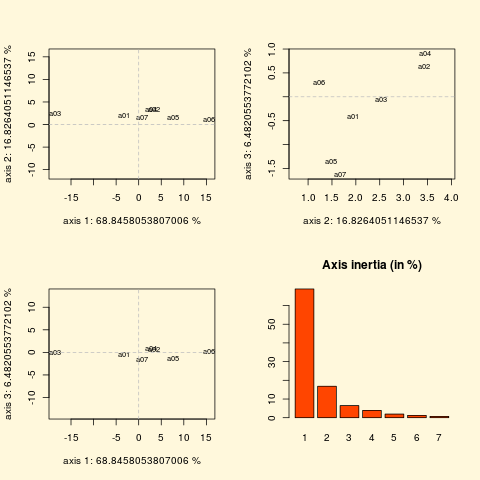
\includegraphics{proWeakOrdering_Colwise.png}
\index{computeWeakOrder() (weakOrders.PrincipalInOutDegreesOrdering method)}

\begin{fulllineitems}
\phantomsection\label{techDoc:weakOrders.PrincipalInOutDegreesOrdering.computeWeakOrder}\pysiglinewithargsret{\bfcode{computeWeakOrder}}{\emph{ColwiseOrder=False}}{}
Specialisation for PrincipalInOutDegreesOrderings.

\end{fulllineitems}

\index{exportGraphViz() (weakOrders.PrincipalInOutDegreesOrdering method)}

\begin{fulllineitems}
\phantomsection\label{techDoc:weakOrders.PrincipalInOutDegreesOrdering.exportGraphViz}\pysiglinewithargsret{\bfcode{exportGraphViz}}{\emph{fileName=None}, \emph{direction='ColwiseOrder'}, \emph{Comments=True}, \emph{graphType='png'}, \emph{graphSize=`7}, \emph{7'}, \emph{fontSize=10}}{}
Specialisation for PincipalInOutDegrees class.

direction = ``Colwise'' (best to worst, default) \textbar{} ``Rowwise'' (worst to best)

\end{fulllineitems}

\index{showPrincipalScores() (weakOrders.PrincipalInOutDegreesOrdering method)}

\begin{fulllineitems}
\phantomsection\label{techDoc:weakOrders.PrincipalInOutDegreesOrdering.showPrincipalScores}\pysiglinewithargsret{\bfcode{showPrincipalScores}}{\emph{ColwiseOrder=False}, \emph{RowwiseOrder=False}}{}
showing the principal in- (Colwise) and out-degrees (Rowwise) scores.

\end{fulllineitems}

\index{showWeakOrder() (weakOrders.PrincipalInOutDegreesOrdering method)}

\begin{fulllineitems}
\phantomsection\label{techDoc:weakOrders.PrincipalInOutDegreesOrdering.showWeakOrder}\pysiglinewithargsret{\bfcode{showWeakOrder}}{\emph{ColwiseOrder=False}}{}
Specialisation for PrincipalInOutDegreesOrderings.

\end{fulllineitems}


\end{fulllineitems}

\index{QsRbcWeakOrdering (class in weakOrders)}

\begin{fulllineitems}
\phantomsection\label{techDoc:weakOrders.QsRbcWeakOrdering}\pysiglinewithargsret{\strong{class }\code{weakOrders.}\bfcode{QsRbcWeakOrdering}}{\emph{argPerfTab=None}, \emph{limitingQuantiles=None}, \emph{LowerClosed=True}, \emph{PrefThresholds=True}, \emph{hasNoVeto=False}, \emph{minValuation=-1.0}, \emph{maxValuation=1.0}, \emph{outrankingType='bipolar'}, \emph{Threading=True}, \emph{cores=None}, \emph{Comments=True}, \emph{Debug=False}}{}
Bases: {\hyperref[techDoc:weakOrders.WeakOrder]{\code{weakOrders.WeakOrder}}}, {\hyperref[techDoc:sortingDigraphs.SortingDigraph]{\code{sortingDigraphs.SortingDigraph}}}

Refinig a quantiles sorting result
with a ranking-by-choosing of the local quantile equivalence classes
of less than 50 items.
For larger quantile equivalence classes, Tideman's ranked pairs heuristic
is used insted.
\begin{description}
\item[{\emph{Parameter}:}] \leavevmode\begin{itemize}
\item {} 
limitingQuantiles are set by default to len(actions)//2
for outranking digraph orders below 200.
For higher orders, centiles are used by default.

\item {} 
threading is on by default for cpu with more than 2 cores.

\end{itemize}

\end{description}

\begin{notice}{note}{Note:}
The weakording is instantiated as strict ordering! And for larger orders
a consistent size of several Giga bytes cpu memory is required.
\end{notice}
\index{computeQsRbcRanking() (weakOrders.QsRbcWeakOrdering method)}

\begin{fulllineitems}
\phantomsection\label{techDoc:weakOrders.QsRbcWeakOrdering.computeQsRbcRanking}\pysiglinewithargsret{\bfcode{computeQsRbcRanking}}{\emph{DescendingOrder=True}, \emph{Comments=False}, \emph{Debug=False}}{}
Render the ranking result of QsRbcWeakOrdering constructor

\end{fulllineitems}

\index{computeWeakOrder() (weakOrders.QsRbcWeakOrdering method)}

\begin{fulllineitems}
\phantomsection\label{techDoc:weakOrders.QsRbcWeakOrdering.computeWeakOrder}\pysiglinewithargsret{\bfcode{computeWeakOrder}}{\emph{DescendingOrder=True}, \emph{Comments=False}, \emph{Debug=False}}{}
specialisation of the showWeakOrder method

\end{fulllineitems}

\index{showActionCategories() (weakOrders.QsRbcWeakOrdering method)}

\begin{fulllineitems}
\phantomsection\label{techDoc:weakOrders.QsRbcWeakOrdering.showActionCategories}\pysiglinewithargsret{\bfcode{showActionCategories}}{\emph{action}, \emph{Debug=False}, \emph{Comments=True}}{}
Renders the union of categories in which the given action is sorted positively or null into.
Returns a tuple : action, lowest category key, highest category key, membership credibility !

\end{fulllineitems}

\index{showActionsSortingResult() (weakOrders.QsRbcWeakOrdering method)}

\begin{fulllineitems}
\phantomsection\label{techDoc:weakOrders.QsRbcWeakOrdering.showActionsSortingResult}\pysiglinewithargsret{\bfcode{showActionsSortingResult}}{\emph{actionSubset=None}}{}
shows the quantiles sorting result all (default) of a subset of the decision actions.

\end{fulllineitems}

\index{showOrderedRelationTable() (weakOrders.QsRbcWeakOrdering method)}

\begin{fulllineitems}
\phantomsection\label{techDoc:weakOrders.QsRbcWeakOrdering.showOrderedRelationTable}\pysiglinewithargsret{\bfcode{showOrderedRelationTable}}{\emph{direction='decreasing'}, \emph{originalRelation=False}}{}
Showing the relation table in decreasing (default) or increasing order.

\end{fulllineitems}

\index{showQsRbcRanking() (weakOrders.QsRbcWeakOrdering method)}

\begin{fulllineitems}
\phantomsection\label{techDoc:weakOrders.QsRbcWeakOrdering.showQsRbcRanking}\pysiglinewithargsret{\bfcode{showQsRbcRanking}}{\emph{DescendingOrder=True}}{}
show the ranking-by-sorting refinement of the quantiles sorting result

\end{fulllineitems}


\end{fulllineitems}

\index{RankingByBestChoosingDigraph (class in weakOrders)}

\begin{fulllineitems}
\phantomsection\label{techDoc:weakOrders.RankingByBestChoosingDigraph}\pysiglinewithargsret{\strong{class }\code{weakOrders.}\bfcode{RankingByBestChoosingDigraph}}{\emph{digraph}, \emph{Normalized=True}, \emph{CoDual=False}, \emph{Debug=False}}{}
Bases: {\hyperref[techDoc:weakOrders.RankingByChoosingDigraph]{\code{weakOrders.RankingByChoosingDigraph}}}

Specialization of abstract WeakOrder class for computing a ranking by best-choosing.
\index{showWeakOrder() (weakOrders.RankingByBestChoosingDigraph method)}

\begin{fulllineitems}
\phantomsection\label{techDoc:weakOrders.RankingByBestChoosingDigraph.showWeakOrder}\pysiglinewithargsret{\bfcode{showWeakOrder}}{}{}
Specialisation of showWeakOrder() for ranking-by-best-choosing results.

\end{fulllineitems}


\end{fulllineitems}

\index{RankingByChoosingDigraph (class in weakOrders)}

\begin{fulllineitems}
\phantomsection\label{techDoc:weakOrders.RankingByChoosingDigraph}\pysiglinewithargsret{\strong{class }\code{weakOrders.}\bfcode{RankingByChoosingDigraph}}{\emph{other}, \emph{fusionOperator='o-max'}, \emph{CoDual=False}, \emph{Debug=False}, \emph{CppAgrum=False}, \emph{Threading=True}}{}
Bases: {\hyperref[techDoc:weakOrders.WeakOrder]{\code{weakOrders.WeakOrder}}}

Specialization of the abstract WeakOrder class for 
ranking-by-Rubis-choosing orderings.

Example python3 session:

\begin{Verbatim}[commandchars=\\\{\}]
\PYG{g+gp}{\PYGZgt{}\PYGZgt{}\PYGZgt{} }\PYG{k+kn}{from} \PYG{n+nn}{outrankingDigraphs} \PYG{k+kn}{import} \PYG{o}{*}
\PYG{g+gp}{\PYGZgt{}\PYGZgt{}\PYGZgt{} }\PYG{n}{t} \PYG{o}{=} \PYG{n}{RandomCBPerformanceTableau}\PYG{p}{(}\PYG{n}{numberOfActions}\PYG{o}{=}\PYG{l+m+mi}{7}\PYG{p}{,}\PYGZbs{} 
\PYG{g+go}{            numberOfCriteria=5,\PYGZbs{} }
\PYG{g+go}{            weightDistribution=\PYGZsq{}equiobjectives\PYGZsq{})}
\PYG{g+gp}{\PYGZgt{}\PYGZgt{}\PYGZgt{} }\PYG{n}{g} \PYG{o}{=} \PYG{n}{BipolarOutrankingDigraph}\PYG{p}{(}\PYG{n}{t}\PYG{p}{,}\PYG{n}{Normalized}\PYG{o}{=}\PYG{n+nb+bp}{True}\PYG{p}{)}
\PYG{g+gp}{\PYGZgt{}\PYGZgt{}\PYGZgt{} }\PYG{n}{g}\PYG{o}{.}\PYG{n}{showRelationTable}\PYG{p}{(}\PYG{p}{)}
\PYG{g+go}{* \PYGZhy{}\PYGZhy{}\PYGZhy{}\PYGZhy{} Relation Table \PYGZhy{}\PYGZhy{}\PYGZhy{}\PYGZhy{}\PYGZhy{}}
\PYG{g+go}{  S   \textbar{}   \PYGZsq{}a01\PYGZsq{}  \PYGZsq{}a02\PYGZsq{}  \PYGZsq{}a03\PYGZsq{}  \PYGZsq{}a04\PYGZsq{}  \PYGZsq{}a05\PYGZsq{}  \PYGZsq{}a06\PYGZsq{}  \PYGZsq{}a07\PYGZsq{}   }
\PYG{g+go}{ \PYGZhy{}\PYGZhy{}\PYGZhy{}\PYGZhy{}\PYGZhy{}\textbar{}\PYGZhy{}\PYGZhy{}\PYGZhy{}\PYGZhy{}\PYGZhy{}\PYGZhy{}\PYGZhy{}\PYGZhy{}\PYGZhy{}\PYGZhy{}\PYGZhy{}\PYGZhy{}\PYGZhy{}\PYGZhy{}\PYGZhy{}\PYGZhy{}\PYGZhy{}\PYGZhy{}\PYGZhy{}\PYGZhy{}\PYGZhy{}\PYGZhy{}\PYGZhy{}\PYGZhy{}\PYGZhy{}\PYGZhy{}\PYGZhy{}\PYGZhy{}\PYGZhy{}\PYGZhy{}\PYGZhy{}\PYGZhy{}\PYGZhy{}\PYGZhy{}\PYGZhy{}\PYGZhy{}\PYGZhy{}\PYGZhy{}\PYGZhy{}\PYGZhy{}\PYGZhy{}\PYGZhy{}\PYGZhy{}\PYGZhy{}\PYGZhy{}\PYGZhy{}\PYGZhy{}\PYGZhy{}\PYGZhy{}\PYGZhy{}\PYGZhy{}\PYGZhy{}\PYGZhy{}\PYGZhy{}\PYGZhy{}\PYGZhy{}\PYGZhy{}\PYGZhy{}\PYGZhy{}\PYGZhy{}}
\PYG{g+go}{\PYGZsq{}a01\PYGZsq{} \textbar{}   +0.00  \PYGZhy{}1.00  \PYGZhy{}1.00  \PYGZhy{}0.33  +0.00  +0.00  +0.00  }
\PYG{g+go}{\PYGZsq{}a02\PYGZsq{} \textbar{}   +1.00  +0.00  \PYGZhy{}0.17  +0.33  +1.00  +0.33  +0.67  }
\PYG{g+go}{\PYGZsq{}a03\PYGZsq{} \textbar{}   +1.00  +0.67  +0.00  +0.33  +0.67  +0.67  +0.67  }
\PYG{g+go}{\PYGZsq{}a04\PYGZsq{} \textbar{}   +0.33  +0.17  \PYGZhy{}0.33  +0.00  +1.00  +0.67  +0.67  }
\PYG{g+go}{\PYGZsq{}a05\PYGZsq{} \textbar{}   +0.00  \PYGZhy{}0.67  \PYGZhy{}0.67  \PYGZhy{}1.00  +0.00  \PYGZhy{}0.17  +0.33  }
\PYG{g+go}{\PYGZsq{}a06\PYGZsq{} \textbar{}   +0.33  +0.00  \PYGZhy{}0.33  \PYGZhy{}0.67  +0.50  +0.00  +1.00  }
\PYG{g+go}{\PYGZsq{}a07\PYGZsq{} \textbar{}   +0.33  +0.00  \PYGZhy{}0.33  \PYGZhy{}0.67  +0.50  +0.17  +0.00  }
\PYG{g+gp}{\PYGZgt{}\PYGZgt{}\PYGZgt{} }\PYG{k+kn}{from} \PYG{n+nn}{weakOrders} \PYG{k+kn}{import} \PYG{n}{RankingByChoosingDigraph}
\PYG{g+gp}{\PYGZgt{}\PYGZgt{}\PYGZgt{} }\PYG{n}{rbc} \PYG{o}{=} \PYG{n}{RankingByChoosingDigraph}\PYG{p}{(}\PYG{n}{g}\PYG{p}{)}
\PYG{g+gp}{\PYGZgt{}\PYGZgt{}\PYGZgt{} }\PYG{n}{rbc}\PYG{o}{.}\PYG{n}{showWeakOrder}\PYG{p}{(}\PYG{p}{)}
\PYG{g+go}{Ranking by Choosing and Rejecting}
\PYG{g+go}{  1st ranked [\PYGZsq{}a03\PYGZsq{}] (0.47)}
\PYG{g+go}{   2nd ranked [\PYGZsq{}a02\PYGZsq{}, \PYGZsq{}a04\PYGZsq{}] (0.58)}
\PYG{g+go}{    3rd ranked [\PYGZsq{}a06\PYGZsq{}] (1.00)}
\PYG{g+go}{    3rd last ranked [\PYGZsq{}a06\PYGZsq{}] (1.00)}
\PYG{g+go}{   2nd last ranked [\PYGZsq{}a07\PYGZsq{}] (0.50)}
\PYG{g+go}{  1st last ranked [\PYGZsq{}a01\PYGZsq{}, \PYGZsq{}a05\PYGZsq{}] (0.58)}
\PYG{g+gp}{\PYGZgt{}\PYGZgt{}\PYGZgt{} }\PYG{n}{rbc}\PYG{o}{.}\PYG{n}{exportGraphViz}\PYG{p}{(}\PYG{l+s}{\PYGZsq{}}\PYG{l+s}{weakOrdering}\PYG{l+s}{\PYGZsq{}}\PYG{p}{)}
\PYG{g+go}{*\PYGZhy{}\PYGZhy{}\PYGZhy{}\PYGZhy{} exporting a dot file for GraphViz tools \PYGZhy{}\PYGZhy{}\PYGZhy{}\PYGZhy{}\PYGZhy{}\PYGZhy{}\PYGZhy{}\PYGZhy{}\PYGZhy{}*}
\PYG{g+go}{Exporting to converse\PYGZhy{}dual\PYGZus{}rel\PYGZus{}randomCBperftab.dot}
\PYG{g+go}{dot \PYGZhy{}Grankdir=BT \PYGZhy{}Tpng converse\PYGZhy{}dual\PYGZus{}rel\PYGZus{}randomCBperftab.dot }
\PYG{g+go}{   \PYGZhy{}o weakOrdering.png }
\end{Verbatim}

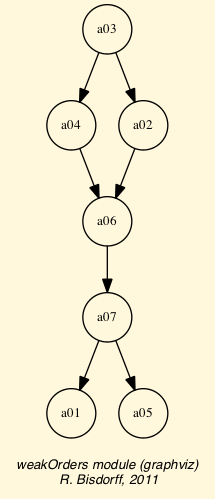
\includegraphics{weakOrdering.png}

\begin{Verbatim}[commandchars=\\\{\}]
\PYG{g+gp}{\PYGZgt{}\PYGZgt{}\PYGZgt{} }\PYG{n}{rbc}\PYG{o}{.}\PYG{n}{showOrderedRelationTable}\PYG{p}{(}\PYG{n}{direction}\PYG{o}{=}\PYG{l+s}{\PYGZdq{}}\PYG{l+s}{decreasing}\PYG{l+s}{\PYGZdq{}}\PYG{p}{)}
\PYG{g+go}{* \PYGZhy{}\PYGZhy{}\PYGZhy{}\PYGZhy{} Relation Table \PYGZhy{}\PYGZhy{}\PYGZhy{}\PYGZhy{}\PYGZhy{}}
\PYG{g+go}{  S   \textbar{}  \PYGZsq{}a03\PYGZsq{}  \PYGZsq{}a04\PYGZsq{}  \PYGZsq{}a02\PYGZsq{}  \PYGZsq{}a06\PYGZsq{}  \PYGZsq{}a07\PYGZsq{}  \PYGZsq{}a01\PYGZsq{}  \PYGZsq{}a05\PYGZsq{}      }
\PYG{g+go}{ \PYGZhy{}\PYGZhy{}\PYGZhy{}\PYGZhy{}\PYGZhy{}\textbar{}\PYGZhy{}\PYGZhy{}\PYGZhy{}\PYGZhy{}\PYGZhy{}\PYGZhy{}\PYGZhy{}\PYGZhy{}\PYGZhy{}\PYGZhy{}\PYGZhy{}\PYGZhy{}\PYGZhy{}\PYGZhy{}\PYGZhy{}\PYGZhy{}\PYGZhy{}\PYGZhy{}\PYGZhy{}\PYGZhy{}\PYGZhy{}\PYGZhy{}\PYGZhy{}\PYGZhy{}\PYGZhy{}\PYGZhy{}\PYGZhy{}\PYGZhy{}\PYGZhy{}\PYGZhy{}\PYGZhy{}\PYGZhy{}\PYGZhy{}\PYGZhy{}\PYGZhy{}\PYGZhy{}\PYGZhy{}\PYGZhy{}\PYGZhy{}\PYGZhy{}\PYGZhy{}\PYGZhy{}\PYGZhy{}\PYGZhy{}\PYGZhy{}\PYGZhy{}\PYGZhy{}\PYGZhy{}\PYGZhy{}\PYGZhy{}\PYGZhy{}\PYGZhy{}\PYGZhy{}\PYGZhy{}\PYGZhy{}\PYGZhy{}\PYGZhy{}\PYGZhy{}\PYGZhy{}\PYGZhy{}}
\PYG{g+go}{\PYGZsq{}a03\PYGZsq{} \textbar{}   \PYGZhy{}      0.33   0.17   0.33   0.33   1.00   0.67     }
\PYG{g+go}{\PYGZsq{}a04\PYGZsq{} \textbar{}  \PYGZhy{}0.33    \PYGZhy{}     0.00   0.67   0.67   0.33   1.00     }
\PYG{g+go}{\PYGZsq{}a02\PYGZsq{} \textbar{}  \PYGZhy{}0.17   0.00    \PYGZhy{}     0.33   0.67   1.00   0.67     }
\PYG{g+go}{\PYGZsq{}a06\PYGZsq{} \textbar{}  \PYGZhy{}0.33  \PYGZhy{}0.67  \PYGZhy{}0.33    \PYGZhy{}     0.17   0.33   0.17     }
\PYG{g+go}{\PYGZsq{}a07\PYGZsq{} \textbar{}  \PYGZhy{}0.33  \PYGZhy{}0.67  \PYGZhy{}0.67  \PYGZhy{}0.17    \PYGZhy{}     0.33   0.33     }
\PYG{g+go}{\PYGZsq{}a01\PYGZsq{} \textbar{}  \PYGZhy{}1.00  \PYGZhy{}0.33  \PYGZhy{}1.00  \PYGZhy{}0.33  \PYGZhy{}0.33    \PYGZhy{}     0.00     }
\PYG{g+go}{\PYGZsq{}a05\PYGZsq{} \textbar{}  \PYGZhy{}0.67  \PYGZhy{}1.00  \PYGZhy{}0.67  \PYGZhy{}0.17  \PYGZhy{}0.33   0.00    \PYGZhy{}       }
\end{Verbatim}
\index{computeRankingByBestChoosing() (weakOrders.RankingByChoosingDigraph method)}

\begin{fulllineitems}
\phantomsection\label{techDoc:weakOrders.RankingByChoosingDigraph.computeRankingByBestChoosing}\pysiglinewithargsret{\bfcode{computeRankingByBestChoosing}}{\emph{Forced=False}}{}
Dummy for blocking recomputing without forcing.

\end{fulllineitems}

\index{computeRankingByLastChoosing() (weakOrders.RankingByChoosingDigraph method)}

\begin{fulllineitems}
\phantomsection\label{techDoc:weakOrders.RankingByChoosingDigraph.computeRankingByLastChoosing}\pysiglinewithargsret{\bfcode{computeRankingByLastChoosing}}{\emph{Forced=False}}{}
Dummy for blocking recomputing without forcing.

\end{fulllineitems}

\index{showRankingByChoosing() (weakOrders.RankingByChoosingDigraph method)}

\begin{fulllineitems}
\phantomsection\label{techDoc:weakOrders.RankingByChoosingDigraph.showRankingByChoosing}\pysiglinewithargsret{\bfcode{showRankingByChoosing}}{\emph{rankingByChoosing=None}}{}
Dummy for showWeakOrder method

\end{fulllineitems}


\end{fulllineitems}

\index{RankingByLastChoosingDigraph (class in weakOrders)}

\begin{fulllineitems}
\phantomsection\label{techDoc:weakOrders.RankingByLastChoosingDigraph}\pysiglinewithargsret{\strong{class }\code{weakOrders.}\bfcode{RankingByLastChoosingDigraph}}{\emph{digraph}, \emph{Normalized=True}, \emph{CoDual=False}, \emph{Debug=False}}{}
Bases: {\hyperref[techDoc:weakOrders.RankingByChoosingDigraph]{\code{weakOrders.RankingByChoosingDigraph}}}

Specialization of abstract WeakOrder class for computing a ranking by rejecting.
\index{showWeakOrder() (weakOrders.RankingByLastChoosingDigraph method)}

\begin{fulllineitems}
\phantomsection\label{techDoc:weakOrders.RankingByLastChoosingDigraph.showWeakOrder}\pysiglinewithargsret{\bfcode{showWeakOrder}}{}{}
Specialisation of showWeakOrder() for ranking-by-last-choosing results.

\end{fulllineitems}


\end{fulllineitems}

\index{RankingByPrudentChoosingDigraph (class in weakOrders)}

\begin{fulllineitems}
\phantomsection\label{techDoc:weakOrders.RankingByPrudentChoosingDigraph}\pysiglinewithargsret{\strong{class }\code{weakOrders.}\bfcode{RankingByPrudentChoosingDigraph}}{\emph{digraph}, \emph{CoDual=False}, \emph{Normalized=True}, \emph{Odd=True}, \emph{Limited=0.2}, \emph{Comments=False}, \emph{Debug=False}, \emph{SplitCorrelation=True}}{}
Bases: {\hyperref[techDoc:weakOrders.RankingByChoosingDigraph]{\code{weakOrders.RankingByChoosingDigraph}}}

Specialization for ranking-by-rejecting results with prudent single elimination of chordless circuits. By default, the cut level for circuits elimination is set to 20\% of the valuation domain maximum (1.0).

\end{fulllineitems}

\index{WeakOrder (class in weakOrders)}

\begin{fulllineitems}
\phantomsection\label{techDoc:weakOrders.WeakOrder}\pysiglinewithargsret{\strong{class }\code{weakOrders.}\bfcode{WeakOrder}}{\emph{file=None}, \emph{order=7}}{}
Bases: {\hyperref[techDoc:digraphs.Digraph]{\code{digraphs.Digraph}}}

Abstract class for weak orderings' specialized methods.
\index{exportDigraphGraphViz() (weakOrders.WeakOrder method)}

\begin{fulllineitems}
\phantomsection\label{techDoc:weakOrders.WeakOrder.exportDigraphGraphViz}\pysiglinewithargsret{\bfcode{exportDigraphGraphViz}}{\emph{fileName=None}, \emph{bestChoice=set()}, \emph{worstChoice=set()}, \emph{noSilent=True}, \emph{graphType='png'}, \emph{graphSize=`7}, \emph{7'}}{}
export GraphViz dot file for digraph drawing filtering.

\end{fulllineitems}

\index{exportGraphViz() (weakOrders.WeakOrder method)}

\begin{fulllineitems}
\phantomsection\label{techDoc:weakOrders.WeakOrder.exportGraphViz}\pysiglinewithargsret{\bfcode{exportGraphViz}}{\emph{fileName=None}, \emph{direction='best'}, \emph{noSilent=True}, \emph{graphType='png'}, \emph{graphSize=`7}, \emph{7'}, \emph{fontSize=10}}{}
export GraphViz dot file for weak order (Hasse diagram) drawing filtering.

\end{fulllineitems}

\index{showOrderedRelationTable() (weakOrders.WeakOrder method)}

\begin{fulllineitems}
\phantomsection\label{techDoc:weakOrders.WeakOrder.showOrderedRelationTable}\pysiglinewithargsret{\bfcode{showOrderedRelationTable}}{\emph{direction='decreasing'}, \emph{originalRelation=False}}{}
Showing the relation table in decreasing (default) or increasing order.

\end{fulllineitems}

\index{showRankingByChoosing() (weakOrders.WeakOrder method)}

\begin{fulllineitems}
\phantomsection\label{techDoc:weakOrders.WeakOrder.showRankingByChoosing}\pysiglinewithargsret{\bfcode{showRankingByChoosing}}{\emph{actionsList=None}, \emph{rankingByChoosing=None}}{}
Dummy name for showWeakOrder() method

\end{fulllineitems}

\index{showWeakOrder() (weakOrders.WeakOrder method)}

\begin{fulllineitems}
\phantomsection\label{techDoc:weakOrders.WeakOrder.showWeakOrder}\pysiglinewithargsret{\bfcode{showWeakOrder}}{\emph{rankingByChoosing=None}}{}
A show method for self.rankinByChoosing result.

\end{fulllineitems}


\end{fulllineitems}


Back to the {\hyperref[techDoc:technical-label]{\emph{Introduction}}}


\subsection{Indices and tables}
\label{techDoc:indices-and-tables}\begin{itemize}
\item {} 
\emph{genindex}

\item {} 
\emph{modindex}

\item {} 
\emph{search}

\end{itemize}


\subsection{Tutorial}
\label{techDoc:tutorial}\begin{itemize}
\item {} 
Tutorial

\end{itemize}


\chapter{Indices and tables}
\label{index:indices-and-tables}\begin{itemize}
\item {} 
\emph{genindex}

\item {} 
\emph{modindex}

\item {} 
\emph{search}

\end{itemize}


\chapter{References}
\label{index:references}
See \href{http://leopold-loewenheim.uni.lu/Digraph3/digraph3\_copyright.html}{Copyright}

\begin{thebibliography}{BIS-2013}
\bibitem[FMCAA]{FMCAA}{\phantomsection\label{tutorial:fmcaa} 
Häggström, Olle \emph{Finite Markov Chians and Algorithmic Applications}. Cambridge University Press 2002.
}
\bibitem[ADT-L2]{ADT-L2}{\phantomsection\label{tutorial:adt-l2} 
Bisdorff, Raymond \emph{Who wins the election}. MICS Algorithmic Decision Theory course, Lecture 2. FSTC/ILIAS University of Luxembourg, Summer Semester 2014 ( downloadable here )
}
\bibitem[BIS-2013]{BIS-2013}{\phantomsection\label{tutorial:bis-2013} \begin{enumerate}
\setcounter{enumi}{17}
\item {} 
Bisdorff (2013) ``On Polarizing Outranking Relations with Large Performance Differences'' \emph{Journal of Multi-Criteria Decision Analysis} (Wiley) \textbf{20}:3-12 (downloadable preprint \href{http://charles-sanders-peirce.uni.lu/bisdorff/documents/MCDA-10-0059-PrePeerReview.pdf}{PDF file} 403.5 Kb).

\end{enumerate}
}
\bibitem[BIS-2008]{BIS-2008}{\phantomsection\label{tutorial:bis-2008} \begin{enumerate}
\setcounter{enumi}{17}
\item {} 
Bisdorff, P. Meyer and M. Roubens (2008) ``RUBIS: a bipolar-valued outranking method for the choice problem''. 4OR, \emph{A Quarterly Journal of Operations Research} Springer-Verlag Volume 6 Number 2 pp. 143-165. (Online) Electronic version: DOI: 10.1007/s10288-007-0045-5 (downloadable preliminary version \href{http://leopold-loewenheim.uni.lu/bisdorff/documents/HyperKernels.pdf}{PDF file 271.5Kb})

\end{enumerate}
}
\end{thebibliography}


\renewcommand{\indexname}{Python Module Index}
\begin{theindex}
\def\bigletter#1{{\Large\sffamily#1}\nopagebreak\vspace{1mm}}
\bigletter{d}
\item {\texttt{digraphs}}, \pageref{techDoc:module-digraphs}
\indexspace
\bigletter{g}
\item {\texttt{graphs}}, \pageref{techDoc:module-graphs}
\indexspace
\bigletter{l}
\item {\texttt{linearOrders}}, \pageref{techDoc:module-linearOrders}
\indexspace
\bigletter{o}
\item {\texttt{outrankingDigraphs}}, \pageref{techDoc:module-outrankingDigraphs}
\indexspace
\bigletter{p}
\item {\texttt{perfTabs}}, \pageref{techDoc:module-perfTabs}
\indexspace
\bigletter{s}
\item {\texttt{sortingDigraphs}}, \pageref{techDoc:module-sortingDigraphs}
\indexspace
\bigletter{v}
\item {\texttt{votingDigraphs}}, \pageref{techDoc:module-votingDigraphs}
\indexspace
\bigletter{w}
\item {\texttt{weakOrders}}, \pageref{techDoc:module-weakOrders}
\end{theindex}

\renewcommand{\indexname}{Index}
\printindex
\end{document}
